\documentclass[11pt,twoside,a4paper,openany]{report}
\usepackage[solcolor]{ex_test} % dethi, color, loigiai, solcolor, book
%\usepackage{ex_test}
\renewtheorem{ex}{\color{blue!60!black} Câu}
	\usepackage[newparttoc]{titlesec}	% định dạng tiêu đề cho các section
\usepackage{titletoc}	% định dạng mục lục 
\usepackage{pdfpages}	% chèn trang từ file pdf 
\usepackage{lipsum}		% văn bản định dạng trang in 
\usepackage[utf8]{vietnam}	% tiếng Việt 
\usepackage{xparse} % hỗ trợ định nghĩa options cho lệnh tự tạo
\usepackage{xcolor,color,colortbl}  % các gói xử lý màu 
\usepackage{xpatch}	% hỗ trợ định nghĩa lệnh tự tạo 
\usepackage{tkz-tab} % xử lý hình với tikz 
\usepackage{fancybox} % tạo các hộp 
\usepackage[most]{tcolorbox} % định dạng các hộp, khung 
\tcbuselibrary{skins} % thư viện bổ sung cho tcolorbox
\usepackage{graphicx} % Chèn hình, vẽ hình đơn giản 
\usepackage{geometry} % định dạng, canh lề trang in 
\usepackage{indentfirst} % viết hoa đoạn đầu của mỗi mục 
\usepackage{fancyhdr} % tạo header và footer 
\usepackage{longtable} % bảng dài nhiều trang 
\usepackage[locale=DE]{siunitx} % cách viết số đo có đơn vị theo chuẩn DE (gần giống VN) 
\usepackage[T1,T5]{fontenc} % font encoding 
\usepackage{tikz} % gói TikZ vẽ hình 
\usetikzlibrary{decorations.shapes,shapes.geometric,calc,positioning}
\usetikzlibrary{ decorations.markings}

\usepackage[version=3]{mhchem} % công thức và phương trình hóa học 
%\usepackage{chemmacros} % công thức ion trong hóa học
%\usepackage{chemfig} % vẽ cấu trúc hợp chất hữu cơ 
\usepackage{wasysym} % các ký hiệu sinh học, khoa học 
\usepackage{makecell} % hỗ trợ định dạng ô trong bảng 
\usepackage{array} % hỗ trợ định dạng array
\usepackage{amsmath,amssymb} % công thức và ký hiệu toán học 
%\usepackage{mathabx} % ký hiệu toán học bổ sung (+ thiên văn)  - xung đột với wasysym, tránh dùng đồng thời 
\usepackage{enumitem} % định dạng môi trường liệt kê 
\setlist[itemize,enumerate,description]{noitemsep, {nosep}}
\usepackage{cprotect}% cho phép marco hủy tác dụng chống verbatim trong các môi trường tiêu đề 
\usepackage{multicol} % môi trường nhiều cột
\usepackage{environ} % hỗ trợ định nghĩa môi trường
\usepackage{tasks} % hỗ trợ list dạng task 
\usepackage{calc} % hỗ trợ tính toán & đo kích thước văn bản 
\usepackage{multido} % thực hiện lệnh lặp lại 
\usepackage{pgf} % hỗ trợ phép tính toán học và vẽ hình	
\usepackage{setspace} % hỗ trợ định dạng khoảng cách văn bản. 
%\usepackage{showframe}	% hiển thị khung lề khi thiết kế
\usepackage{tabularx} % hỗ trợ bảng 
\usepackage{needspace} % hỗ trợ định dạng khối dòng văn bản 
\usepackage{hyperref}
% định dạng tham chiếu và tham chiếu chéo 
\hypersetup{hidelinks,colorlinks=false,breaklinks=true,bookmarksopen=true}
%\usepackage{slashbox}	% chia chéo trong bảng
%\usepackage{mnsymbol} % tạo thêm symbol (stars)

%\usepackage[varg]{txfonts}	% hỗ trợ font 
%\usepackage{times}			% font Times (kèm txfonts)
%\usepackage{helvet}			% font helvet (không chân - kèm txfonts)

\usepackage{capt-of}
\usepackage{tikz}
\usepackage{multirow}
\usepackage{pgfplots}
\usetikzlibrary{
	pgfplots.fillbetween,
}
\pgfplotsset{compat=1.13}
\usetikzlibrary{decorations.markings,bending}
\usetikzlibrary{shapes.geometric}
\usepackage{tkz-euclide}
\usepackage{fontawesome}
\usepackage{circuitikz}
	%============ DECLARATION OF DEFAULT VALUE =====
\def\SDTi{09.0354.0608}
\def\SDTii{09.6175.0612}
\newcommand{\outfooter}{
	{\color{purple}\faPhoneSquare\, \SDTi \,\,--\,\, \faPhoneSquare\ \SDTii} % Tên tài liệu ở footer
}

\graphicspath{{../figs/}{../extra/}} % các thư mục chứa hình ảnh 

% ========== PAPER FORMAT ====================
% --- paper size 
\geometry{
	a4paper	% khổ giấy A4
	,total={180mm,260mm} % kích thước văn bản A4 170mmx247mm
	,left=15mm % canh lề trái
	,top=15mm % canh lề trên
	,footskip=1.0cm % khoảng cách từ văn bản đến footer
}
% --- line spacing -- choose 1 in 2 choices 
\onehalfspacing			% cách dòng đơn
%\doublespacing			% cách dòng đôi  

% ========== color =============
\definecolor{obcolor}{HTML}	
%		{ffce00}	% Mathematics
{aa98ff}	% Physics
%		{99bcff}	% Chemistry
%		{c4e538}	% Biology
%		{f37676}	% English
% --- testing
\colorlet{pagecol}{white}	

\colorlet{headerbcol}{obcolor}
\colorlet{headerdcol}{black}
\colorlet{headertcol}{black}

\colorlet{footercol}{obcolor}
\colorlet{footertextcol}{black}

\colorlet{secdcol}{black}
\colorlet{secbcol}{obcolor}
\colorlet{sectcol}{black}
\colorlet{secnbcol}{white}
\colorlet{secntcol}{black}

\colorlet{ssecdcol}{black}
\colorlet{ssectcol}{black}
\colorlet{ssecnbcol}{obcolor}
\colorlet{ssecntcol}{black}

\colorlet{dangtbcol}{obcolor!15}

\colorlet{vidufcol}{obcolor}
\colorlet{vidutbcol}{obcolor}
\colorlet{viduttcol}{black}
\colorlet{vidumbcol}{pagecol}
\colorlet{vidumtcol}{black}
\colorlet{vidulbcol}{pagecol}
\colorlet{vidultcol}{black}

\colorlet{baitapfcol}{obcolor}
\colorlet{baitaptbcol}{obcolor}
\colorlet{baitapttcol}{black}
\colorlet{baitapmbcol}{obcolor!15}
\colorlet{baitapmtcol}{black}
\colorlet{baitaplbcol}{pagecol}
\colorlet{baitapltcol}{black}

\colorlet{stardrawcol}{white}
\colorlet{starmkdcol}{white}
\colorlet{starempcol}{vidutbcol}

\definecolor{manatbcol}{HTML}{05C88C}
\colorlet{manatfcol}{manatbcol}
\colorlet{manafcol}{manatbcol!25}
\colorlet{manambcol}{manafcol}

\definecolor{luuytbcol}{HTML}{546de5}
\colorlet{luuytfcol}{luuytbcol}
\colorlet{luuyfcol}{luuytbcol!25}
\colorlet{luuymbcol}{luuyfcol}

\definecolor{pphaptbcol}{HTML}{f45b5b}
\colorlet{pphaptfcol}{pphaptbcol}
\colorlet{pphapfcol}{pphaptbcol!25}
\colorlet{pphapmbcol}{pphapfcol}

\pagecolor{pagecol}

% ========== DEFINE LEVELS  
% --- định nghĩa môi trường \mychapter, nằm giữa \part và \chapter
\titleclass{\mychapter}{top}[\part] 
\newcounter{mychapter}[part]
\renewcommand{\themychapter}{\arabic{mychapter}}
\titlespacing{\mychapter}{0pt}{1cm}{2.3em}


% ========== MAIN TABLE OF CONTENTS =========
\contentsmargin{1.5em}	
\titlecontents{part}
[3cm] % Left indentation
{\addvspace{20pt}
	\begin{tikzpicture}[remember picture, overlay]%
		\draw[fill=obcolor!70!black,draw=black] (-2.4,-.15) rectangle (0,.5);%
		\pgftext[left,x=-2.2cm,y=0.15cm]{\color{white}\sc\bfseries \textbf{CHƯƠNG}  \thecontentslabel};%
	\end{tikzpicture}\color{black!60}\large\bfseries\hspace*{1pt}
} % Spacing and font options for parts
{}
{}
{}
[\addvspace{5pt}\color{black}]
% My chapter text styling 
\titlecontents{mychapter}
[1.25em]
{}
{ CHỦ ĐỀ \thecontentslabel.\enspace}
{}
{\titlerule*[0.75pc]{.}\contentspage} %bad formatting, but only here to produce a content line in ToC	
% Chapter text styling
\titlecontents{chapter}
[1.25cm] % Left indentation
{} % Spacing and font options for chapters
{} % Formatting of numbered sections of this type
{} % Formatting of numberless sections of this type
{\nolinebreak\;\titlerule*[.75pc]{.}\;\contentspage} % Formatting of the filler to the right of the heading and the page number

\makeatletter
% that a section has Level 2, rather than Level 1.
\renewcommand{\l@section}{\@dottedtocline{2}{1.5em}{2.3em}}
\makeatother
\setcounter{tocdepth}{1}

% ========== TITLE FORMATTING 
% --- draw circle around chapter number 
\newcommand*{\circhap}[1]{
	\tikz[baseline=(char.base)] % tạo ô bao quanh chữ
	{
		\node[
		shape=circle % hình tròn
		,fill=gray!50 % màu nền 
		,inner sep=5pt % khoảng cách chữ và hình 
		] 
		(char)
		{#1};
	}
}	
% --- 
\AtBeginDocument{
	% --- PART format (level -1)
	\titleclass{\part}{top}
	\renewcommand{\thepart}{\arabic{part}}
	\titleformat{\part}
	[display]
	{\bfseries\Huge}
	{\filleft \LARGE PHẦN  \Huge\thepart}
	{4ex}
	{\titlerule
		%\pagecolor{green}	 
		\vspace{2ex}%
		\filcenter
	}
	[\vspace{2ex}%
	\titlerule
	%\pagecolor{white}
	]
	
	% --- MYCHAPTER format (level 0) 
	\titleformat{\mychapter}
	[display]
	{\bfseries\huge}
	{\filleft \LARGE\itshape Chủ đề \Huge\themychapter}
	{4ex}
	{%\titlerule
		\vspace{2ex}%
		\filcenter}
	[\vspace{2ex}%
	%\titlerule
	]
	
	% --- CHAPTER format (level 1)
	\titleformat{\chapter}
	[display]
	{\normalfont\large\bfseries\centering}
	{}
	{-3.5cm} % giảm khoảng cách của chapter đến đầu trang
	{\Large}	
	%\titleformat % định dạng tiêu đề
	\renewcommand{\thesection} % định dạng chỉ số subsection
	{
		\arabic{section} % kiểu số Ả rập
	}
	\titleformat{\section} % chỉnh tiêu đề section  
	[hang]
	{\large\bfseries} % format 
	{\thesection\!\!.} % không ghi chỉ mục 
	{0.5em} % khoảng cách đến tiêu đề 
	{} % trước khi bắt đầu 
	\renewcommand{\thesubsection} % định dạng chỉ số subsection
	{
		\thesection\!\!.\,\arabic{subsection} % kiểu số Ả rập 
	}
	\titleformat % định dạng tiêu đề 
	{\subsection} %command 
	{\normalsize\bfseries} % format 
	{\thesubsection\!\!.} % đánh số 1,2,3,...
	{0.5em} % khoảng cách đến tiêu đề 
	{} % trước tiêu đề 
	[] % sau tiêu đề 	
	\renewcommand{\thesubsubsection} % định dạng chỉ số subsubsection 
	{
		\thesubsection\!\!.\,\arabic{subsubsection} % kiểu số Ả rập 
	}
	\titleformat % định dạng tiêu đề 
	{\subsubsection} % command 
	{\normalsize\bfseries} % format 
	{\thesubsubsection\!\!.} % 1.1, 1.2
	{0.25em} % khoảng cách sau 1.1 
	{ } % trước tiêu đề 
	[\vspace*{-3mm}] % sau tiêu đề  	
}


% ----- định dạng Header và footer
% --- trang văn bản thông thường  
\pagestyle{fancy} 
\fancyhf{}
\renewcommand{\headrulewidth}
{0pt} % độ dày đường kẻ ở header 
\newcommand*\cirpage[1] % tạo hình tròn quanh số trang 
{\tikz[baseline=(char.base)]
	{
		\node[
		shape=circle
		,draw=black
		,fill=gray!0
		,inner sep=2pt
		]
		(char)
		{#1};
	}
}
\fancyfoot[LO,RE] % footer - lề trong 
{	
	\small \outfooter % tên tài liệu lấy từ phần khai báo đầu file 
}  
\fancyfoot[CO,CE] % footer - giữa trang 
{
	\small \cirpage{\thepage}
} 
\fancyfoot[LE] % footer - lề ngoài 
{
	\vspace*{-11pt}
	\hspace*{-1.1pt}\text{\bfseries\color{purple} Lớp vật lý Cô Thảo - Thầy Sang}
}
\fancyfoot[RO] % footer - lề ngoài 
{
	\vspace*{-11pt}
	\text{\bfseries\color{purple} Lớp vật lý Cô Thảo - Thầy Sang}
}
% --- trang Part và terter title 
\fancypagestyle{plain} % mặc định của trang Part và Chapter title 
{
	\fancyfoot[LO,RE]
	{
		\small \outfooter
	}
	\fancyfoot[CO,CE]
	{
		\small \cirpage{\thepage}
	} % footer - giữa trang chẵn và lẻ 
	\fancyfoot[LE]
	{
		\vspace*{-11pt}
		\hspace*{-1.1pt}\text{\bfseries\color{purple} Lớp vật lý Cô Thảo - Thầy Sang}
	}
	\fancyfoot[RO]
	{
		\vspace*{-11pt}
		\text{\bfseries\color{purple} Lớp vật lý Cô Thảo - Thầy Sang}
	}
} % giống với trang thường 


% --- Định dạng cấu trúc 
\setcounter{secnumdepth}{4} % đánh số đến cấp thứ 4 của chỉ mục (subsubsection sẽ được đánh số)






% ======== MANUAL DEFINITIONS VERSION 3.1415 ===
% --- chừa chỗ trống tương ứng - văn bản gốc 
\newcommand{\bltext}[1]{#1}
\newcommand{\xtrule}{ }
\newcommand{\phantomeqn}[2][b]{
	#2
}


% --- tạo hộp Tóm tắt lý thuyết  
\newcommand{\hops}[1] %lệnh hộp (tóm tắt lý thuyết)
{	
	\begin{flushright}
		\leavevmode 
		\begin{tcolorbox}
			[
			standard jigsaw
			,opacityback=0
			,opacityframe=1
			,breakable
			,pad at break*=2mm
			%						,colback=white!20!white,
			,colframe=black!70!white
			,width=\textwidth
			,before upper={\parindent15pt}
			%						,watermark color=blue!3!white
			%						,watermark text=\arabic{tcbbreakpart}
			]
			{
				#1
			}
		\end{tcolorbox}
	\end{flushright}
}

% --- định nghĩa môi trường mới - Dạng 
\newcounter{dang} % định nghĩa chỉ số cho Dạng 
[section] % chỉ số sẽ reset mỗi section 
\newenvironment % định nghĩa môi trường mới 
{dang} % tên môi trường 
[1] % số thành phần phải có 
{
	\refstepcounter{dang} % chỉ số tương ứng 
	\leavevmode
	\begin{center}
		\leavevmode \vspace{-0.6cm}
		\begin{tcolorbox}
			[
			bicolor
			,sidebyside
			,width=0.98\textwidth
			,lefthand width=2.4cm
			,arc=0.5cm
			%	,rounded corners
			,colback=blue!3
			,colbacklower=green!4
			,segmentation engine=path
			,segmentation style=
			{
				line width=1.5pt
				,solid
			}
			%						,borderline={0.3mm}{0.3mm}{black}
			]
			\large
			{
				\bf Mục tiêu \thedang
			}
			\tcblower
			\centering\large
			{
				\color{white}\large\bfseries #1
			}
		\end{tcolorbox}
	\end{center}
	
} 

{
	
	\par
	\medskip	
}

% --- Định nghĩa lệnh tạo box Phương pháp giải 
\newcommand{\ppgiai}[1] %lệnh hộp (tóm tắt lý thuyết)
{
	\leavevmode 
	\begin{center}
		\leavevmode 
		\begin{tcolorbox}
			[
			%standard jigsaw
			,enhanced
			,opacityback=0
			,opacityfill=1
			,attach boxed title to top left={yshift=-3mm,yshifttext=-1mm}
			,boxed title style=
			{
				size=small
				,boxrule=1.5pt
				,colframe=black!70!white
				,colback=white!10!black
			}
			,title=\textbf{Phương pháp giải}
			%						,opacityback=0
			,opacityframe=1
			,breakable
			,pad at break*=2mm
			,colback=green!3,
			,colframe=black!70!white
			,width=0.85\textwidth
			,before upper={\parindent15pt}
			%						,watermark color=blue!3!white
			%						,watermark text=\arabic{tcbbreakpart}
			]
			{
				#1
			}
		\end{tcolorbox}
	\end{center}
}

% --- Định nghĩa lệnh tạo box Manatips
\newcommand{\manatip}[1] %lệnh hộp (tóm tắt lý thuyết)
{	\begin{center}
		\leavevmode 
		\begin{tcolorbox}
			[
			%standard jigsaw
			,enhanced
			,opacityback=0
			,opacityfill=1
			,attach boxed title to top left={yshift=-0.5mm,yshifttext=0mm}
			,boxed title style=
			{
				size=small
				,boxrule=1.5pt
				,colframe=black!70!white
				,colback=white!40!black
			}
			,title=\textbf{Tip}
			%						,opacityback=0
			,opacityframe=1
			,breakable
			,pad at break*=2mm
			,colback=white!20!white,
			,colframe=black!70!white
			,width=0.85\textwidth
			,before upper={\parindent15pt}
			%						,watermark color=blue!3!white
			%						,watermark text=\arabic{tcbbreakpart}
			]
			{
				#1
			}
		\end{tcolorbox}
	\end{center}
}
% --- Định nghĩa lệnh tạo box Lưu ý khi dàn trang
\newcommand{\notebox}[1] %lệnh hộp (tóm tắt lý thuyết)
{	\begin{center}
		\leavevmode 
		\begin{tcolorbox}
			[
			%standard jigsaw
			,enhanced
			,opacityback=0
			,opacityfill=1
			,attach boxed title to top center={yshift=-0.5mm,yshifttext=0mm}
			,boxed title style=
			{
				size=small
				,boxrule=1.5pt
				,colframe=red!90!white
				,colback=red!90!white
			}
			,title=\textbf{Lưu ý khi dàn trang}
			%						,opacityback=0
			,opacityframe=1
			,breakable
			,pad at break*=2mm
			,colback=red!20!white,
			,colframe=red!90!white
			,width=0.85\textwidth
			,before upper={\parindent15pt}
			%						,watermark color=blue!3!white
			%						,watermark text=\arabic{tcbbreakpart}
			]
			{
				#1
			}
		\end{tcolorbox}
	\end{center}
}

% --- Định nghĩa lệnh tạo box Lưu ý 
\newcommand{\luuy}[1] %lệnh hộp (tóm tắt lý thuyết)
{	
	\vspace*{-0.7cm}
	\begin{center}
		\leavevmode 
		\begin{tcolorbox}
			[
			%standard jigsaw
			,enhanced
			,opacityback=0
			,opacityfill=1
			,attach boxed title to top right={yshift=-0.5mm,yshifttext=0mm}
			,boxed title style=
			{
				size=small
				,boxrule=1.5pt
				,colframe=black!70!white
				,colback=purple!
			}
			,title=\textbf{Lưu ý}
			%						,opacityback=0
			,opacityframe=1
			,breakable
			,pad at break*=2mm
			,colback=white!20!white,
			,colframe=black!70!white
			,width=0.85\textwidth
			,before upper={\parindent15pt}
			%						,watermark color=blue!3!white
			%						,watermark text=\arabic{tcbbreakpart}
			]
			{
				#1
			}
		\end{tcolorbox}
	\end{center}
}



% --- Tạo môi trường các đáp án trắc nghiệm 
\makeatletter
\@ifpackagelater{tasks}{2019/10/04}
{
	\NewTasksEnvironment[style=enumerate,label=\Alph*.,label-format={\bfseries},label-width=2ex,label-offset=1ex,item-indent=1.8cm]{mcq}[\item](1)
	% Code which runs if the package date is 2019/10/04 or later
}
{
	\NewTasks[style=enumerate,counter-format={\bfseries tsk[A].},label-width=2ex,label-offset=1.5ex,item-indent=1.8cm]{mcq}[\item](1)
	% Code which runs if the package date is older than 2019/10/04
}
\makeatother
%	\NewEnviron{mcq}[1][]
%		{
	% Misc. stuff to preceed the tasks env here
	%			\def\tempbegin
	%				{%\vspace{1cm}
		%					\begin{twopartasks}
			%				}%
		%					\expandafter\tempbegin\BODY
		%					\end{twopartasks}
	% Misc. stuff to follow
	%		}

% -- insert stars
\newcommand\score[2]{%
	\pgfmathsetmacro\pgfxa{#1 + 1}%
	\tikzstyle{scorestars}=[star, star points=5, star point ratio=2.25, draw, inner sep=1.75pt, anchor=outer point 3]%
	\begin{tikzpicture}[baseline]
		\foreach \i in {1, ..., #2} {
			\pgfmathparse{\i<=#1 ? "black" : "white"}
			\edef\starcolor{\pgfmathresult}
			\draw (\i*2.5ex, 0ex) node[name=star\i, scorestars, fill=\starcolor]  {};
		}
	\end{tikzpicture}%
}
\newcommand{\mkstar}[1]{\protect\score{#1}{4}}


% --- Định nghĩa môi trường ví dụ 
\newcommand{\vidu}[3] % -- không đánh số, có lời giải 
{
	%\vspace{0.3cm}
	\noindent\textbf{Ví dụ}\quad\mkstar{#1}
	\needspace{4\baselineskip}
	\begin{flushright}
		\leavevmode\vspace{-15pt}
		\begin{tcolorbox}[
			standard jigsaw
			,opacityback=0
			,opacityframe=0
			,width=0.95\textwidth
			,breakable
			,right=-4pt,top=-4pt,left=-4pt
			,colframe=white
			,colback=white
			,before upper={\parindent15pt}
			]
			
			{#2}
			\needspace{4\baselineskip}
			%			\begin{center}
				%				\textbf{Giải:}
				%			\end{center}
			
			{#3}	
		\end{tcolorbox}
	\end{flushright}	
}

\newcommand{\viduon}[2] % không đánh số, không lời giải
{
	%\vspace{0.3cm}
	\noindent\textbf{Ví dụ \quad\mkstar{#1}}
	\needspace{4\baselineskip}
	\begin{flushright}
		\leavevmode\vspace{-15pt}
		\begin{tcolorbox}[
			standard jigsaw
			,opacityback=0
			,opacityframe=0
			,width=0.95\textwidth
			,breakable
			,right=-4pt,top=-4pt,left=-4pt
			,colframe=white
			,colback=white
			,before upper={\parindent15pt}
			]
			
			
			{#2}
			
		\end{tcolorbox}
	\end{flushright}	
}

\newcounter{viduii}[dang] % chỉ số của ví dụ, reset khi bắt đầu dạng mới 
\newcommand{\viduii}[3] % có đánh số, có lời giải 
{
	\refstepcounter{viduii}
	\begin{tcolorbox}[
		title=\textbf{\textsf{Ví dụ \theviduii~}}\hfill \mkstar{#1}
		,width=0.9\linewidth
		,grow to right by=0.1\textwidth
		%		,text width=0.9/textwidth
		,breakable
		,colbacktitle=vidutbcol
		,coltitle=viduttcol
		,colframe=vidufcol
		,colback=vidumbcol
		,boxrule=1.5pt
		,every float=\centering
		]
		{#2}
		\tcblower
		{\begin{center}
				\textbf{Hướng dẫn giải}
			\end{center}
			#3}
	\end{tcolorbox}
	\vspace{5pt}
}


\newcommand{\viduin}[2] % có đánh số, không lời giải 
{
	%\vspace{0.3cm}
	\refstepcounter{viduii}
	\needspace{4\baselineskip}
	\noindent\textbf{Ví dụ \theviduii~ \quad\mkstar{#1}}
	\begin{flushright}
		\leavevmode\vspace{-10pt}
		\begin{tcolorbox}[
			standard jigsaw
			,opacityback=0
			,opacityframe=0
			,width=0.95\textwidth
			,breakable
			,right=-4pt,top=-4pt,left=-4pt
			,colframe=white
			,colback=white
			,before upper={\parindent15pt}
			]
			
			
			{#2}	
			
		\end{tcolorbox}
	\end{flushright}	
}

% --- các ký tự tạo thêm 
% --- ký hiệu song song 
\newcommand{\parallelsum} % tên lệnh tạo ký hiệu song song 
{
	{\mathbin{\!/\mkern-5mu/\!}}
}
\newcommand{\dpara}{\parallelsum}
% --- đồng nhất kí hiệu độ (đơn vị góc) thành ^\circ
\renewcommand{\ang}[1]{#1^\circ}
% --- ký hiệu suất điện động và công suất như sgk
% ký hiệu từ font Boondox 
\DeclareFontFamily{U}{BOONDOX-cal}{\skewchar\font=45 }
\DeclareFontShape{U}{BOONDOX-cal}{m}{n}{
	<-> s*[1.05] BOONDOX-r-cal}{}
\DeclareFontShape{U}{BOONDOX-cal}{b}{n}{
	<-> s*[1.05] BOONDOX-b-cal}{}
\DeclareMathAlphabet{\bdx}{U}{BOONDOX-cal}{m}{n}
\SetMathAlphabet{\bdx}{bold}{U}{BOONDOX-cal}{b}{n}
\DeclareMathAlphabet{\bbdx}{U}{BOONDOX-cal}{b}{n}
\newcommand{\calE}{\bdx{E}}
\newcommand{\calP}{\bdx{P}}
% lệnh siunit 
\newcommand{\xsi}[2]{\SI[parse-numbers=false]{#1}{#2}}

% --- định nghĩa môi trường định luật 
\newtheorem{thrPh}{Định luật}

%--- hỗ trợ bảng 
\renewcommand{\theadfont}
{
	\normalfont\bfseries
} % làm ô trong bảng canh giữa + in đậm 
\newcommand{\nfhead}[1] % tên lệnh 
{
	\renewcommand{\theadfont}
	{
		\normalfont
	}
	\thead{#1}
	\renewcommand{\theadfont}
	{
		\normalfont\bfseries
	} 
} % làm ô trong bảng canh giữa 
% lưu ý, khi sử dụng \thead và \nfhead thì phải xuống dòng thủ công.

% --- tạo dòng trống 
\newcommand{\Pointilles}[1]{%
	\par\nobreak
	\noindent\rule{0pt}{\baselineskip}% Provides a larger gap between the preceding paragraph and the dots
	%\doublespacing
	\multido{}{#1}{\noindent\makebox[\linewidth]{\dotfill}\endgraf}% ... dotted lines ...
	%\onehalfspacing
	\bigskip% Gap between dots and next paragraph
}

\newcommand{\Linesfill}[1]{%
	\par\nobreak
	\noindent\rule{0pt}{\baselineskip}% Provides a larger gap between the preceding paragraph and the dots
	%\doublespacing
	\multido{}{#1}{\noindent\rule{\linewidth}{0.2pt}\endgraf}% ... dotted lines ...
	%\onehalfspacing
	\bigskip% Gap between dots and next paragraph
}	

\newcommand{\Blfill}[1]{%
	\par\nobreak
	\noindent\rule{0pt}{\baselineskip}% Provides a larger gap between the preceding paragraph and the dots
	%\doublespacing
	\multido{}{#1}{\noindent\rule{\linewidth}{0pt}\endgraf}% ... dotted lines ...
	%\onehalfspacing
	\bigskip% Gap between dots and next paragraph
}	

\newcommand{\phantomline}[2][b]{
	\ifx b#1 \Blfill{#2} \else
	\ifx d#1	\Pointilles{#2} \else
	\ifx l#1 \Linesfill{#2}
	\fi\fi\fi 
}

% --- các lệnh che các đoạn văn bản 
\newlength{\saveparindent}
\AtBeginDocument{\setlength{\saveparindent}{\parindent}}

\newsavebox{\mytext}

\newcommand{\dotshide}[1]{%
	\savebox{\mytext}{%
		\parbox[t]{\columnwidth}{
			\setlength{\parindent}{\saveparindent}
			#1\par\xdef\savedprevdepth{\the\prevdepth}
		}%
	}%
	\doublespacing
	\noindent
	\pgfmathparse{int(round(\the\dp\mytext/\the\baselineskip))}
	\Pointilles{\pgfmathresult}
	\par
	% restore \prevdepth to compute correctly the interline glue
	\prevdepth\savedprevdepth
}

\newcommand{\lineshide}[1]{%
	\savebox{\mytext}{%
		\parbox[t]{\columnwidth}{
			\setlength{\parindent}{\saveparindent}
			#1\par\xdef\savedprevdepth{\the\prevdepth}
		}%
	}%
	\noindent
	%	\vrule height \ht\mytext % the height of \mytext
	%	depth \dp\mytext  % the depth of \mytext
	%	width \columnwidth
	%	\newline	
	\pgfmathparse{int(round(\the\dp\mytext/\the\baselineskip))}
	\Linesfill{\pgfmathresult}
	\par
	% restore \prevdepth to compute correctly the interline glue
	\prevdepth\savedprevdepth
}

\newcommand{\blankhide}[1]{%
	\savebox{\mytext}{%
		\parbox[t]{\columnwidth}{
			\setlength{\parindent}{\saveparindent}
			#1\par\xdef\savedprevdepth{\the\prevdepth}
		}%
	}%
	\noindent
	\pgfmathparse{int(round(\the\dp\mytext/\the\baselineskip))}
	\Blfill{\pgfmathresult}
	\par
	% restore \prevdepth to compute correctly the interline glue
	\prevdepth\savedprevdepth
}

\newcommand{\hide}[2][b]{
	\ifx b#1 #2
	\fi
}

% --- new commands workshop 
\DeclareSIUnit\minute{\textrm{phút}}
% 
\newcommand{\bai}[1]{\part{#1}}
\newcommand{\LO}[1]{\chapter{#1}}

% --- equation number
\renewcommand{\theequation}{\arabic{equation}}


% --- testing 
\newcommand{\hides}[1]{#1}
% --- các lệnh bật / tắt dáp án
\newcommand{\AnswersOff}{
	\def\anskey{0}
}
\newcommand{\AnswersOn}{
	\def\anskey{1}
}	
\newcommand{\hideall}[1]{
	#1}
\renewcommand{\hideall}[1]{
	\ifthenelse{\equal{\anskey}{0}}{}{
		#1}	
}

% --- tạo minitoc cho part, mychapter 
\newcommand{\startPartToc}{
	\startcontents[part]
	\printcontents[part]{}{0}{\setcounter{tocdepth}{0}}
}
\newcommand{\stopPartToc}{\stopcontents[part]}
\newcommand{\startMyChapterToc}{
	\startcontents[mychapter]
	\printcontents[mychapter]{}{0}{\setcounter{tocdepth}{1}}	
}
\newcommand{\stopMyChapterToc}{\stopcontents[mychapter]}
% --- bỏ xuống dòng trong title ở ToC 
%	\let\oldchapter\chapter
\newcommand{\phantomlesson}[1]{}

% --- figure counter according to mychapter
\counterwithout{figure}{chapter}
\counterwithin{figure}{mychapter}

\newcommand{\hdc}[1]{
	\begin{center}
		\textbf{HƯỚNG DẪN CHẤM}
	\end{center}
	#1}
\renewcommand{\hdc}[1]{
	\ifthenelse{\equal{\anskey}{0}}{}{
		\begin{center}
			\textbf{HƯỚNG DẪN CHẤM}
		\end{center}
		#1}	
}

\newcommand{\ANSMCQ}[1]{
	\begin{center}
		\textbf{BẢNG ĐÁP ÁN}
	\end{center}
	#1}
\renewcommand{\ANSMCQ}[1]{
	\ifthenelse{\equal{\anskey}{0}}{}{
		\begin{center}
			\textbf{BẢNG ĐÁP ÁN}
		\end{center}
		#1}	
}

\newcolumntype{M}[1]{>{\centering\arraybackslash}m{#1}} % m là middle
\newcolumntype{C}[1]{>{\centering\arraybackslash}p{#1}} 
\newcolumntype{L}[1]{>{\raggedright\arraybackslash}p{#1}}
\newcommand{\hoac}[2]{ %hệ hoặc
	\left[\begin{aligned}&#1\\
		&#2\end{aligned}\right.}





%	% --- tạo đường kẻ chấm 
	\newcommand{\dhorline}[2]{\hbox to #1{\leaders\hbox to 0.5em{\hss . \hss}\hfil}}
	
% --- chừa chỗ trống tương ứng trong câu 
	
	\newlength\rulegoal
	\newlength\drule
	\setlength{\drule}{0.5em}
	\newcommand\breakableruleaux[2]{%
		\ifdim\rulegoal>\drule\relax%
		\dhorline{\drule}{#2}\allowbreak%
		\def\next{\breakableruleaux{#1}{#2}}%
		\else
		\dhorline{\rulegoal}{#2}%
		\def\next{}%
		\fi 
		\addtolength{\rulegoal}{-\drule}%
		\next%
	}
	
	\newcommand\breakablerule[2]{\setlength{\rulegoal}{#1}\breakableruleaux{#1}{#2}}
	
	\newlength{\myblanklength}
	\renewcommand{\bltext}[1]
	{
		~\hspace*{-7.5pt}\relax
		\settowidth{\myblanklength}{#1}
		\breakablerule{\the\myblanklength*\real{1.5}}{0.2pt}
	}
	
	\renewcommand{\xtrule}{\hspace*{-5pt}\dhorline{1cm}{0.2pt}~}
	
% --- % che công thức trên dòng riêng:
\renewcommand{\phantomeqn}[1]{
	%		\phantomline[b]{1} % dòng trắng
	\phantomline[d]{1} % dòng kẻ chấm
	%		\phantomline[l]{1} % dòng kẻ liền
}

% che đoạn văn bản 
	
	\renewcommand{\hide}[2][b]{
		\ifx b#1 \blankhide{#2} \else
		\ifx d#1 \dotshide{#2} \else
		\ifx l#1 \lineshide{#2}
		\fi\fi\fi 
	}

% che bài giải tất cả ví dụ 
%\usetikzlibrary{decorations.shapes}
%	\tikzset{

%		decoration = {shape backgrounds, shape=circle,

%			shape size=0.25pt, shape sep=2pt},

%		paint/.style = {decorate, fill=black}

%		}% tạo dạng dots 

	\renewcommand{\vidu}[3] % -- không đánh số, có lời giải 
		{
			%\vspace{0.3cm}
			\needspace{4\baselineskip}
			\noindent\textbf{Ví dụ \quad\ \mkstar{#1}}
			\begin{flushright}
				\leavevmode\vspace{-15pt}
				\begin{tcolorbox}[
					standard jigsaw
					,opacityback=0
					,opacityframe=0
					,width=0.95\textwidth
					,breakable
					,right=-4pt,top=-4pt,left=-4pt
					,colframe=white
					,colback=white
					,before upper={\parindent15pt}
					]
				
					{#2}
				\end{tcolorbox}
			
				\begin{tcolorbox}
					[enhanced
					,frame hidden
					,width=0.95\textwidth
					,borderline={0.3mm}{0.5mm}{dotted}
					,colback=white
					,title=Bài giải
					,fonttitle=\bfseries
					,coltitle=black
					,breakable
					,attach boxed title to top center={yshift=-\tcboxedtitleheight/2}
					,boxed title style={colback=green!10!white}]
					\hide{#3}
				\end{tcolorbox}	
				
			\end{flushright}	
		}
	
	\renewcommand{\viduii}[3] % có đánh số, có lời giải 
		{
			%\vspace{0.3cm}
			\refstepcounter{viduii}
			\needspace{4\baselineskip}
			\noindent\textbf{Ví dụ \theviduii\ \mkstar{#1}}
			\begin{flushright}
				\leavevmode\vspace{-15pt}
				\begin{tcolorbox}[
					standard jigsaw
					,opacityback=0
					,opacityframe=0
					,width=0.95\textwidth
					,breakable
					,right=-4pt,top=-4pt,left=-4pt
					,colframe=white
					,colback=white
					,before upper={\parindent15pt}
					]
					
					
					{#2}
				\end{tcolorbox}
					%\begin{center}
					%	\textbf{Giải:}
					%\end{center}
					
				\begin{tcolorbox}
					[enhanced
					,width=0.95\textwidth
					,frame hidden
					,borderline={0.3mm}{0.5mm}{dotted}
					,colback=white
					,title=Bài giải
					,fonttitle=\bfseries
					,coltitle=black
					,breakable
					,attach boxed title to top center={yshift=-\tcboxedtitleheight/2}
					,boxed title style={colback=green!10!white}]
					\hide{#3}
				\end{tcolorbox}	
			\end{flushright}	
		}
	

\begin{document}
	
%	\tableofcontents
%	\cleardoublepage
	\AnswersOn
%	\AnswersOff
% ==================================LỚP 11 =================================================
%	\setcounter{part}{0}
%	\part{TỔNG HỢP KIẾN THỨC}
%	\startcontents[parts]
%	\printcontents[parts]{}{0}{\setcounter{tocdepth}{0}}
%	\setcounter{mychapter}{-1}
%	\mychapter{CHUYÊN ĐỀ TRƯỜNG HẤP DẪN}
%	\startcontents[mychapters]
%	\printcontents[mychapters]{}{0}{\setcounter{tocdepth}{1}}
%	\begin{center}
%		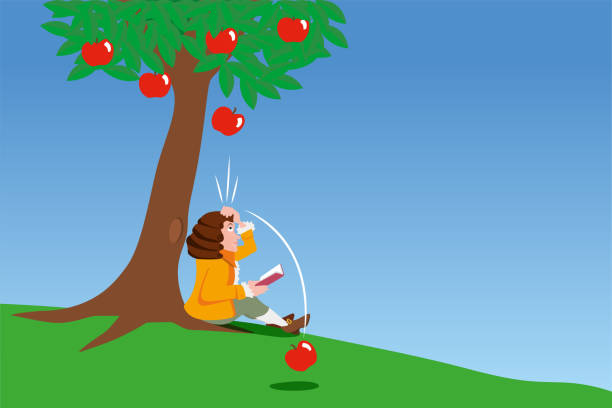
\includegraphics[scale=1.5]{../figs/11C0}
%	\end{center}
%	\chapter{Tóm tắt lý thuyết và công thức}
\section{Định luật vạn vật hấp dẫn}
Lực hấp dẫn giữa hai chất điểm tỉ lệ thuận với tích hai khối lượng và tỉ lệ nghịch với bình phương khoảng cách giữa chúng.
$$F_\text{hấp dẫn}=G\dfrac{m_Am_B}{r^2}$$
với:
\begin{itemize}
	\item $m_A$, $m_B$: khối lượng hai chất điểm, đơn vị trong hệ SI là kilogram $\left(\si{\kilogram}\right)$,
	\item $r$: khoảng cách giữa hai chất điểm, đơn vị trong hệ SI là mét $\left(\si{\meter}\right)$,
	\item $G$: hằng số hấp dẫn, có giá trị thực nghiệm $G=\SI{6.68E-11}{\dfrac{\newton\meter^2}{\kilogram^2}}$.
\end{itemize}
\section{Trường hấp dẫn}
\subsection{Định nghĩa}
Trường hấp dẫn là trường vật chất bao quanh một vật có khối lượng và là môi trường truyền tương tác giữa các vật có khối lượng. Tính chất cơ bản của trường hấp dẫn là tác dụng lực hấp dẫn lên vật có khối lượng khác đặt trong nó.
\subsection{Tính chất}
Trường hấp dẫn của một vật khối lượng $M$ có các tính chất:
\begin{itemize}
	\item Tương tác hấp dẫn là tương tác hút.
	\item Các đường sức của trường hấp dẫn luôn hướng vào tâm của vật sinh ra trường hấp dẫn.
	\item Phạm vi tác dụng của trường hấp dẫn rất lớn. Tuy nhiên, càng ra xa vật $M$ thì độ lớn của lực hấp dẫn càng giảm.
	\item Trường hấp dẫn chỉ được xem gần đúng là trường đều khi xét trong vùng không gian rất nhỏ.
\end{itemize}
\section{Cường độ trường hấp dẫn}
Cường độ trường hấp dẫn là đại lượng đặc trưng cho trường hấp dẫn về phương diện tác dụng lực lên các vật có khối lượng đặt trong trường hấp dẫn.
$$g=\dfrac{GM}{r^2}$$
với:
\begin{itemize}
	\item $G$: hằng số hấp dẫn, có giá trị thực nghiệm $G=\SI{6.68E-11}{\dfrac{\newton\meter^2}{\kilogram^2}}$,
	\item $M$: khối lượng vật thể gây ra trường hấp dẫn, đơn vị trong hệ SI là kilogram $\left(\si{\kilogram}\right)$,
	\item $r$: khoảng cách từ chất điểm $M$ đến điểm đang xét, đơn vị trong hệ SI là mét $\left(\si{\meter}\right)$.
\end{itemize}
Nếu xem Trái Đất dạng hình cầu đồng nhất khối lượng $M_\text{TĐ}$ và bán kính $R_\text{TĐ}$ thì cường độ trường hấp dẫn của một điểm trên mặt cầu này là
$$g=G\dfrac{M_\text{TĐ}}{\left(R_\text{TĐ}+h\right)^2}$$
Tại điểm ở gần mặt đất $\left(h=0\right)$ thì
$$g_0=G\dfrac{M_\text{TĐ}}{R^2_\text{TĐ}}\approx\SI{9.81}{\meter/\second^2}.$$
\section{Thế năng hấp dẫn - Thế hấp dẫn}
\subsection{Thế năng hấp dẫn}
Thế năng hấp dẫn là đại lượng đặc trưng cho năng lượng tương tác hấp dẫn giữa vật có khối lượng $M$ và vật có khối lượng $m$.\\
Thế năng hấp dẫn tại một điểm trong trường hấp dẫn do vật có khối lượng $M$ sinh ra là công cần thực hiện để dịch chuyển một vật có khối lượng $m$ từ điểm đó ra xa vô cùng
$$W=-G\dfrac{mM}{r}$$
với $r$ là khoảng cách giữa hai vật.
\subsection{Thế hấp dẫn}
Thế hấp dẫn tại một điểm trong trường hấp dẫn của một vật có khối lượng $M$ gây ra là đại lượng đặc trưng cho khả năng tạo ra thế năng hấp dẫn cho các vật khác đặt tại điểm đó
$$\Phi=-G\dfrac{M}{r}$$
với $r$ là khoảng cách từ $M$ đến điểm đang xét.\\
Thế năng hấp dẫn của vật có khối lượng $m$ đặt tại một điểm trong trường hấp dẫn được xác định
$$W=m\Phi.$$
%	\chapter{Câu hỏi ôn tập}
\Opensolutionfile{ans}[ans/Y23-VN11-PH-C0-Q-TN]
% ===================================================================
\begin{ex}
	Câu nào sau đây là đúng khi nói về lực hấp dẫn do Trái Đất tác dụng lên Mặt Trời và do Mặt Trời tác dụng lên Trái Đất?
	\choice
	{Hai lực này cùng phương, cùng chiều}
	{Hai lực này cùng chiều, cùng độ lớn}
	{\True Hai lực này cùng phương, ngược chiều, cùng độ lớn}
	{Phương của hai lực này luôn thay đổi và không trùng nhau}
	\loigiai{}
\end{ex}
% ===================================================================
\begin{ex}
Với $G$ là hằng số hấp dẫn, $M$ là khối lượng Trái Đất, $R$ là bán kính Trái Đất, $h$ là độ cao của vật nặng, $m$ là khối lượng vật nặng thì gia tốc rơi tự do của một vật ở gần mặt đất được tính bởi công thức	
	\choice
	{\True $g=\dfrac{GM}{R^2}$}
	{$g=\dfrac{GM}{\left(R+h\right)^2}$}
	{$g=\dfrac{GMm}{R^2}$}
	{$g=\dfrac{GMm}{\left(R+h\right)^2}$}
	\loigiai{}
\end{ex}
% ===================================================================
\begin{ex}
	Đơn vị của hằng số hấp dẫn là
	\choice
	{$\si{\kilogram\meter/\second^2}$}
	{\True $\si{\newton\meter^2/\kilogram^2}$}
	{$\si{\meter/\second^2}$}
	{$\si{\newton\meter/\second}$}
	\loigiai{}
\end{ex}
% ===================================================================
\begin{ex}
	Hai tàu thuỷ, mỗi chiếc có khối lượng 50000 tấn ở cách nhau $\SI{1}{\kilo\meter}$. So sánh lực hấp dẫn giữa chúng với trọng lượng của một quả cân có khối lượng $\SI{20}{\gram}$. Lấy $g=\SI{10}{\meter/\second^2}$.
	\choice
	{\True Nhỏ hơn}
	{Bằng nhau}
	{Lớn hơn}
	{Chưa đủ dữ kiện để xác định}
	\loigiai{Lực hấp dẫn giữa hai tàu thuỷ:
		$$F=\dfrac{Gm^2}{r^2}=\left(\SI{6.68E-11}{\newton\meter^2/\kilogram^2}\right)\cdot\dfrac{\left(\SI{5E7}{\kilogram}\right)^2}{\left(\SI{1000}{\meter}\right)^2}=\SI{0.167}{\newton}$$
		Trọng lượng của vật nặng $\SI{20}{\gram}$:
		$$P=mg=\left(\SI{20E-3}{\kilogram}\right)\cdot\left(\SI{10}{\meter/\second^2}\right)=\SI{0.2}{\newton}$$
		Vậy lực hấp dẫn giữa hai tàu thuỷ nhỏ hơn trọng lượng của vật có khối lượng $\SI{20}{\gram}$.
	}
\end{ex}
% ===================================================================
\begin{ex}
	Chọn phát biểu \textbf{sai}.
	\choice
	{Các hành tinh đều chuyển động trên các quỹ đạo elip với mặt trời là một tiêu điểm}
	{Coi quỹ đạo chuyển động của các hành tinh gần đúng là tròn thì lực hấp dẫn tác dụng lên hành tinh đã gây ra gia tốc hướng tâm}
	{Tốc độ tối thiểu để đưa vệ tinh lên quỹ đạo tròn quanh Trái Đất là tốc độ vũ trụ cấp I}
	{\True Nếu tốc độ đầu để đưa vệ tinh lên quỹ đạo lớn hơn tốc độ vũ trụ cấp I thì vệ tinh sẽ đi xa khỏi Trái Đất theo quỹ đao parabol}
	\loigiai{Đáp án D sai vì nếu tốc độ đầu của vệ tinh lớn hơn tốc độ vũ trụ cấp I nhưng chưa đạt đến tốc độ vũ trụ cấp II thì vệ tinh chưa thoát ra khỏi trường hấp dẫn của Trái Đất, do đó nó sẽ chuyển động xung quanh Trái Đất.}
\end{ex}
% ===================================================================
\begin{ex}
	Khi khối lượng của hai vật và khoảng cách giữa chúng đều giảm đi phân nửa thì lực hấp dẫn giữa chúng có độ lớn 
	\choice
	{giảm đi 8 lần}
	{giảm đi một nửa}
	{\True giữ nguyên như cũ}
	{tăng gấp đôi}
	\loigiai{$$\dfrac{F'}{F}=\dfrac{m'_1m'_2}{m_1m_2}\cdot\left(\dfrac{r}{r'}\right)^2=\dfrac{1}{4}\cdot2^2=1$$}
\end{ex}
% ===================================================================
\begin{ex}
	Chỉ ra kết luận \textbf{sai} trong các kết luận sau đây
	\choice
	{Trọng lực của một vật được xem gần đúng là lực hút của Trái Đất tác dụng lên vật đó}
	{Trọng lực có chiều hướng về phía Trái Đất}
	{Trọng lực của một vật giảm khi đưa vật lên cao hoặc đưa vật từ cực bắc trở về xích đạo}
	{\True Trên Mặt Trăng, nhà du hành vũ trụ có thể nhảy lên rất cao so với khi nhảy ở Trái Đất vì ở đó khối lượng và trọng lượng của nhà du hành giảm}
	\loigiai{Khi lên Mặt Trăng, gia tốc trọng trường giảm dẫn đến trọng lượng của nhà du hành giảm, khối lượng của nhà du hành không thay đổi.}
\end{ex}
% ===================================================================
\begin{ex}
	Một vật ở trên mặt đất có trọng lượng $\SI{9}{\newton}$. Khi ở một điểm cách tâm Trái Đất $3R$ ($R$ là bán kính Trái Đất) thì nó có trọng lượng là
	\choice
	{$\SI{81}{\newton}$}
	{$\SI{27}{\newton}$}
	{$\SI{3}{\newton}$}
	{\True $\SI{1}{\newton}$}
	\loigiai{$$\dfrac{P'}{P}=\dfrac{g'}{g}=\left(\dfrac{r}{r'}\right)^2=\left(\dfrac{1}{3}\right)^2=\dfrac{1}{9}\Rightarrow P'=\dfrac{P}{9}=\SI{1}{\newton}.$$}
\end{ex}
% ===================================================================
\begin{ex}
Gia tốc rơi tự do ở bề mặt Mặt Trăng là $g_0$ và bán kính Mặt Trăng là $\SI{1740}{\kilo\meter}$. Ở độ cao $h=\SI{3480}{\kilo\meter}$ so với bề mặt Mặt Trăng thì gia tốc rơi tự do bằng	
	\choice
	{\True $g_0/9$}
	{$g_0/3$}
	{$3g_0$}
	{$9g_0$}
	\loigiai{$$\dfrac{g}{g_0}=\left(\dfrac{R}{R+h}\right)^2=\left(\dfrac{\SI{1740}{\kilo\meter}}{\SI{1740}{\kilo\meter}+\SI{3480}{\kilo\meter}}\right)^2=\dfrac{1}{9}\Rightarrow g=\dfrac{g_0}{9}.$$}
\end{ex}
% ===================================================================
\begin{ex}
	Biết bán kính Trái Đất là $R$. Lực hút của Trái Đất đặt vào một vật khi vật đó ở trên mặt đất là $\SI{45}{\newton}$. Khi lực hút do Trái Đất tác dụng lên vật là $\SI{5}{\newton}$ thì vật ở độ cao bằng
	\choice
	{\True $2R$}
	{$9R$}
	{$\dfrac{2R}{3}$}
	{$\dfrac{R}{9}$}
	\loigiai{$$\dfrac{F'}{F}=\left(\dfrac{R}{R+h}\right)^2\Leftrightarrow \dfrac{R}{R+h}=\dfrac{1}{3}\Rightarrow h=2R.$$}
\end{ex}
% ===================================================================
\begin{ex}
	Hãy tính gia tốc rơi tự do trên bề mặt của Mộc Tinh. Biết gia tốc rơi tự do trên bề mặt Trái Đất là $g=\SI{9.81}{\meter/\second^2}$, khối lượng của Mộc Tinh bằng 318 lần khối lượng của Trái Đất, đường kính của Mộc Tinh và của Trái Đất lần lượt là $\SI{142980}{\kilo\meter}$ và $\SI{12750}{\kilo\meter}$.
	\choice
	{$\SI{278.2}{\meter/\second^2}$}
	{\True $\SI{24.8}{\meter/\second^2}$}
	{$\SI{3.88}{\meter/\second^2}$}
	{$\SI{6.2}{\meter/\second^2}$}
	\loigiai{Gia tốc rơi tự do ở bề mặt hành tinh
		$$g=\dfrac{GM}{R^2}$$
		Như vậy:
		$$\dfrac{g'}{g}=\dfrac{M_\text{Mộc Tinh}}{M_\text{TĐ}}\cdot\left(\dfrac{R_\text{TĐ}}{R_\text{Mộc Tinh}}\right)^2=\dfrac{M_\text{Mộc Tinh}}{M_\text{TĐ}}\cdot\left(\dfrac{D_\text{TĐ}}{D_\text{Mộc Tinh}}\right)^2=318\cdot\left(\dfrac{\SI{12750}{\kilo\meter}}{\SI{142980}{\kilo\meter}}\right)^2=2,53$$
		$$\Rightarrow g'=\SI{24.8}{\meter/\second^2}.$$}
\end{ex}
% ===================================================================
\begin{ex}
	Người ta phóng một con tàu vũ trụ từ Trái Đất bay về hướng Mặt Trăng. Biết rằng khoảng cách từ tâm Trái Đất đến tâm Mặt Trăng gấp 60 lần bán kính $R$ của Trái Đất, khối lượng của Mặt Trăng nhỏ hơn khối lượng Trái Đất 81 lần. Hỏi ở cách tâm Trái Đất là bao nhiêu thì lực hút của Trái Đất và của Mặt Trăng lên con tàu vũ trụ sẽ cân bằng nhau?
	\choice
	{$50R$}
	{$60R$}
	{\True $54R$}
	{$6R$}
	\loigiai{Gọi $R_1$ là khoảng cách từ tàu vũ trụ đến tâm Trái Đất và $R_2$ là khoảng cách từ tàu vũ trụ đến tâm Mặt Trăng.\\
		Lực hút của Trái Đất và của Mặt Trăng lên con tàu vũ trụ cân bằng nhau thì
		\begin{equation}
			\label{eq:1}
			G\dfrac{mM_\text{TĐ}}{R^2_1}=G\dfrac{mM_\text{MT}}{R^2_2}\Rightarrow \dfrac{R_1}{R_2}=\sqrt{\dfrac{M_\text{TĐ}}{M_\text{MT}}}=9
		\end{equation}
		Mà 
		\begin{equation}
			\label{eq:2}
			R_1+R_2=60R
		\end{equation}
		Từ (\ref{eq:1}) và (\ref{eq:2}) ta thu được $R_1=54R$ và $R_2=6R$.}
\end{ex}
% ===================================================================
\begin{ex}
	Một vệ tinh chuyển động tròn quanh tâm Trái Đất với bán kính quỹ đạo $\SI{6600}{\kilo\meter}$ với chu kì 89 phút. Biết hằng số hấp dẫn $G=\SI{6.67E-11}{\dfrac{\newton\meter^2}{\kilogram^2}}$. Khối lượng Trái Đất là
	\choice
	{$\SI{5E20}{\kilogram}$}
	{\True $\SI{6E24}{\kilogram}$}
	{$\SI{3E25}{\kilogram}$}
	{$\SI{8E26}{\kilogram}$}
	\loigiai{Vệ tinh chuyển động tròn xung quanh tâm Trái Đất, lực hấp dẫn do Trái Đất tác dụng lên vệ tinh đóng vai trò là lực hướng tâm
		$$F_\text{hd}=ma_\text{ht}$$
		$$\Leftrightarrow G\dfrac{mM}{R^2}=m\omega^2R=m\cdot\left(\dfrac{2\pi}{T}\right)^2R$$
		$$\Rightarrow M=\dfrac{1}{G}\cdot\left(\dfrac{2\pi}{T}\right)^2R^3\approx
		\SI{5.97E24}{\kilogram}$$}
\end{ex}
% ===================================================================
\begin{ex}
	Trái Đất quay quanh Mặt Trời trên một quỹ đạo gần tròn có bán kính trung bình $\SI{150E6}{\kilo\meter}$. Biết khối lượng của Mặt Trời là $\SI{1.97E30}{\kilogram}$. Lấy $G=\SI{6.67E-11}{\dfrac{\newton\meter^2}{\kilogram^2}}$. Với các dữ kiện như trên thì chuyển động của Trái Đất quanh Mặt Trời là bao lâu?
	\choice
	{365 ngày}
	{366 ngày}
	{367 ngày}
	{\True 368 ngày}
	\loigiai{Lực hấp dẫn do Mặt Trời tác dụng lên Trái Đất đóng vai trò là lực hướng tâm làm cho Trái Đất chuyển động trên quỹ đạo tròn xung quanh Mặt Trời
		$$F_\text{hd}=ma_\text{ht}$$
		$$\Leftrightarrow G\dfrac{mM_S}{R^2}=m\omega^2R=m\cdot\left(\dfrac{2\pi}{T}\right)^2R$$
		$$\Rightarrow T=\sqrt{\dfrac{4\pi^2R^3}{GM_S}}\approx\SI{31.84E6}{\second}=368,56\ \text{ngày}.$$}
\end{ex}
% ===================================================================
\begin{ex}
	Một vệ tinh chuyển động trên quỹ đạo tròn bán kính bằng nửa bán kính quỹ đạo của Mặt Trăng quay xung quanh Trái Đất. Biết chu kì quay của Mặt Trăng xung quanh Trái Đất là 27,5 ngày. Chu kì quay của vệ tinh nói trên xung quanh Trái Đất là bao lâu?
	\choice
	{5,3 ngày}
	{6,4 ngày}
	{8,2 ngày}
	{\True 9,7 ngày}
	\loigiai{Vệ tinh chuyển động tròn xung quanh tâm Trái Đất, lực hấp dẫn do Trái Đất tác dụng lên vệ tinh đóng vai trò là lực hướng tâm
		$$F_\text{hd}=ma_\text{ht}$$
		$$\Leftrightarrow G\dfrac{mM}{R^2}=m\omega^2R=m\cdot\left(\dfrac{2\pi}{T}\right)^2R$$
		$$\Rightarrow \dfrac{T^2}{R^3}=\dfrac{4\pi^2}{GM}=const$$
		Như vậy:
		$$\dfrac{T^2_\text{vệ tinh}}{R^3_\text{vệ tinh}}=\dfrac{T^2_\text{MT}}{R^3_\text{MT}}\Rightarrow T_\text{vệ tinh}=T_\text{MT}\cdot\left(\dfrac{R_\text{vệ tinh}}{R_\text{MT}}\right)^{\dfrac{3}{2}}=T_\text{MT}\left(\dfrac{1}{2}\right)^{\dfrac{3}{2}}\approx 9,7\ \text{ngày}.$$}
\end{ex}
\Closesolutionfile{ans}
%	\stopcontents[mychapters]
%	\mychapter{DAO ĐỘNG}
%	\startcontents[mychapters]
%	\printcontents[mychapters]{}{0}{\setcounter{tocdepth}{1}}
%	\begin{center}
%		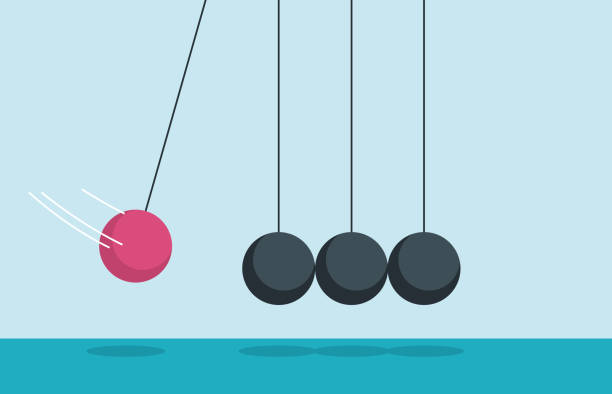
\includegraphics[scale=1.5]{../figs/11C1}
%	\end{center}
%	\chapter{Tóm tắt lý thuyết}
\section{Mô tả dao động}
\subsection{Định nghĩa dao động cơ, dao động tuần hoàn và dao động điều hoà}
\begin{itemize}
	\item Dao động cơ là sự chuyển động qua lại quanh vị trí cân bằng.
	\item Dao động tuần hoàn là dao động mà trạng thái chuyển động của vật được lặp lại như cũ sau những khoảng thời gian bằng nhau.
	\item Dao động điều hoà là dao động tuần hoàn mà li độ của vật dao động là một hàm cosin (hoặc sin) theo thời gian.
\end{itemize}
\subsection{Chu kỳ, tần số, pha dao động, tần số góc}
\begin{itemize}
	\item Chu kì dao động là khoảng thời gian để vật thực hiện được một dao động:
	$$T=\dfrac{\Delta t}{N}.$$
	Trong đó $N$ là số dao động toàn phần thực hiện được trong khoảng thời gian $\Delta t$.\\
	Trong hệ SI, chu kì có đơn vị là giây $\left(\si{\second}\right)$.
	\item Tần số dao động là số dao động toàn phần mà vật thực hiện được trong một giây:
	$$f=\dfrac{1}{T}=\dfrac{N}{\Delta t}.$$
	Trong hệ SI, tần số có đơn vị là Hertz $\left(\si{\hertz}\right)$.
	\item Pha dao động là đại lượng đặc trưng cho trạng thái của vật trong quá trình dao động.
	\item Tần số góc của dao động là đại lượng đặc trưng cho tốc độ biến thiên của pha dao động. Đối với dao động điều hoà, tần số góc có giá trị không đổi và được xác định bằng:
	$$\omega=\dfrac{\Delta\varphi}{\Delta t}=\dfrac{2\pi}{T}.$$
	Trong hệ SI, tần số góc có đơn vị là radian trên giây $\left(\si{\radian/\second}\right)$.
\end{itemize}
\section{Phương trình dao động điều hoà}
\subsection{Li độ}
Phương trình li độ của vật dao động điều hoà:
$$x=A\cos\left(\omega t+\varphi_0\right)$$
Trong đó:
\begin{itemize}
	\item $x$: li độ dao động (toạ độ của vật mà gốc toạ độ được chọn trùng với VTCB), đơn vị trong hệ SI là mét $\left(\si{\meter}\right)$;
	\item $A$: biên độ dao động (giá trị cực đại của li độ), đơn vị trong hệ SI là mét $\left(\si{\meter}\right)$;
	\item $\omega$: tần số góc, đơn vị trong hệ SI là radian trên giây $\left(\si{\radian/\second}\right)$;
	\item $\varphi_0$: pha ban đầu, đơn vị trong hệ SI là radian $\left(\si{\radian}\right)$.
\end{itemize}
\subsection{Phương trình vận tốc}
$$v=-\omega A\sin\left(\omega t+\varphi_0\right)=\omega A\cos\left(\omega t+\varphi_0\right)$$
\begin{itemize}
	\item Vật ở VTCB $\left(x=0\right)$, vật đạt tốc độ cực đại: $v_\text{max}=\omega A$;
	\item Vật ở vị trí biên $\left(x=\pm A\right)$, vật đạt tốc độ cực tiểu $v=0$.
\end{itemize}
\subsection{Gia tốc}
$$a=-\omega^2A\cos\left(\omega t+\varphi_0\right)=-\omega^2x$$
\begin{itemize}
	\item Vật ở VTCB $\left(x=0\right)$: $a=0$;
	\item Vật ở biên $\left(x=\pm A\right)$, gia tốc có độ lớn cực đại $\left|a\right|=\omega^2 A$
	\begin{itemize}
		\item Vật ở vị trí biên dương $\left(x=A\right)$, gia tốc cực tiểu: $a_\text{min}=-\omega^2A$;
		\item Vật ở biên âm $\left(x=-A\right)$, gia tốc cực đại: $a_\text{max}=\omega^2 A$.
	\end{itemize}
\end{itemize}
\section{Năng lượng trong dao động điều hoà}
\begin{itemize}
	\item Thế năng:
	$$W_\text{t}=\dfrac{1}{2}Kx^2=\dfrac{1}{2}m\omega^2A^2\cos^2\left(\omega t+\varphi_0\right)$$
	\item Động năng:
	$$W_\text{đ}=\dfrac{1}{2}mv^2=\dfrac{1}{2}m\omega^2A^2\sin^2\left(\omega t+\varphi_0\right)$$
	\item Cơ năng:
	$$W=W_\text{t}+W_\text{đ}=\dfrac{1}{2}m\omega^2A^2$$
\end{itemize}
\section{Dao động tắt dần và hiện tượng cộng hưởng}
\subsection{Dao động tắt dần}
Dao động tắt dần là dao động có biên độ giảm dần theo thời gian.
\subsection{Dao động cưỡng bức}
Dao động của vật dưới tác dụng của ngoại lực điều hoà trong giai đoạn ổn định được gọi là dao động cưỡng bức. Ngoại lực điều hoà tác dụng vào vật khi này được gọi là lực cưỡng bức.\\
\textit{Tần số góc của vật dao động cưỡng bức bằng tần số góc của ngoại lực cưỡng bức.}
\subsection{Hiện tượng cộng hưởng}
Hiện tượng cộng hưởng xảy ra khi tần số góc của lực cưỡng bức bằng tần số góc riêng của hệ dao động. Khi này, biên độ dao động cưỡng bức của hệ đạt giá trị cực đại $A_\text{max}$.\\
\textit{Tuỳ trường hợp mà hiện tượng cộng hưởng có thể có lợi hoặc có thể có hại.}
%	\chapter{Tóm tắt công thức}
\section{Chu kì, tần số, tần số góc của vật dao động điều hoà}
$$T=\dfrac{\Delta t}{N},\quad f=\dfrac{N}{\Delta t}=\dfrac{1}{T}, \quad \omega=\dfrac{\Delta \varphi}{\Delta t}=\dfrac{2\pi}{T}=2\pi f.$$
\section{Phương trình dao động điều hoà}
\subsection{Phương trình li độ}
$$x=A\cos\left(\omega t+\varphi_0\right)$$
\subsection{Phương trình vận tốc}
$$v=-\omega A\sin\left(\omega t+\varphi_0\right)=\omega A\cos\left(\omega t+\varphi_0\right)$$
$$v_\text{max}=\omega A$$
\subsection{Phương trình gia tốc}
$$a=-\omega^2A\cos\left(\omega t+\varphi_0\right)=-\omega^2x$$
$$a_\text{max}=\omega^2A=\omega v_\text{max}$$
\section{Quãng đường đi được}
\begin{itemize}
	\item Quãng đường đi được trong 1 chu kì dao động: $s=4A$,
	\item Quãng đường đi được trong $N$ chu kì dao động: $s=N\cdot4A$,
	\item Quãng đường đi được trong nửa chu kì dao động: $s=2A$,
	\item Quãng đường cực đại/cực tiểu trong khoảng thời gian $\Delta t<\dfrac{T}{2}$:
	$$s_\text{max}=2A\sin\dfrac{\omega \Delta t}{2}, \quad S_\text{min}=2A\left(1-\cos\dfrac{\omega \Delta t}{2}\right).$$
\end{itemize}
\section{Mối liên hệ giữa các đại lượng trong dao động điều hoà}
\begin{itemize}
	\item Vận tốc sớm pha $\xsi{\dfrac{\pi}{2}}{\radian}$ so với li độ:
	$$\left(\dfrac{x}{A}\right)^2+\left(\dfrac{v}{v_\text{max}}\right)^2=1\Leftrightarrow x^2+\dfrac{v^2}{\omega^2}=A^2.$$
	\item Gia tốc ngược pha với li độ:
	$$a=-\omega^2x$$
	\item Gia tốc sớm pha $\xsi{\dfrac{\pi}{2}}{\radian}$ so với vận tốc: 
	$$\left(\dfrac{a}{a_\text{max}}\right)^2+\left(\dfrac{v}{v_\text{max}}\right)^2=1\Leftrightarrow \dfrac{v^2}{\omega^2}+\dfrac{a^2}{\omega^4}=A^2.$$
\end{itemize}
\section{Một số dao động điều hoà thường gặp}
\subsection{Con lắc lò xo}
\subsubsection{Chu kì, tần số, tần số góc}
$$\omega=\sqrt{\dfrac{k}{m}},\quad T=2\pi\sqrt{\dfrac{m}{k}},\quad f=\dfrac{1}{2\pi}\sqrt{\dfrac{k}{m}}$$
\subsubsection{Năng lượng dao động}
\begin{align*}
	W_\text{t}&=\dfrac{1}{2}kx^2=\dfrac{1}{2}m\omega^2x^2=\dfrac{1}{2}m\omega^2A^2\cos^2\left(\omega t+\varphi_0\right)\\
	W_\text{đ}&=\dfrac{1}{2}mv^2=\dfrac{1}{2}m\omega^2A^2\sin^2\left(\omega t+\varphi_0\right)\\
	W&=W_\text{t}+W_\text{đ}=\dfrac{1}{2}m\omega^2A^2
\end{align*}
\subsubsection{Lực đàn hồi và lực kéo về}
$$F_\text{đh}=-k\Delta\ell,\quad F_\text{kv}=-kx$$
\subsubsection{Chiều dài lò xo}
Chọn gốc toạ độ tại vị trí cân bằng của vật nặng, chiều dương cùng chiều lò xo dãn.
\begin{itemize}
	\item \textbf{\textit{Con lắc lò xo nằm ngang}}
	\begin{itemize}
		\item Ở VTCB lò xo không biến dạng: $\Delta\ell_0=0$;
		\item Ở vị trí li độ $x$, độ biến dạng của lò xo: $\Delta\ell=x$;
		\item Chiều dài lò xo:
		\begin{align*}
			\ell=\ell_0+x\Rightarrow
			\begin{cases}
				\ell_\text{max}=\ell_0+A\\
				\ell_\text{min}=\ell_0-A
			\end{cases}
		\Rightarrow 
		\begin{cases}
			\ell_0=\dfrac{\ell_\text{max}-\ell_\text{min}}{2}\\
			A=\dfrac{\ell_\text{max}-\ell_\text{min}}{2}
		\end{cases}
		\end{align*}
		\item Độ lớn lực đàn hồi:\\
		$$F_\text{đh max}=kA\ \text{(vật ở biên)}, \quad F_\text{đh min}=0\ \text{(vật ở VTCB)}.$$
	\end{itemize}
\item \textbf{\textit{Con lắc lò xo treo thẳng đứng}}
\begin{itemize}
	\item Ở VTCB lò xo bị dãn: $\Delta\ell_0=\dfrac{mg}{k}$;
	\item Ở vị trí li độ $x$, độ biến dạng của lò xo: $\Delta\ell=\Delta\ell_0+x$;
	\item Chiều dài lò xo: $$, $$;
	\begin{align*}
		\begin{cases}
			\ell_\text{CB}=\ell_0+\Delta\ell_0\\
			\ell=\ell_\text{CB}+x
		\end{cases}
		\Rightarrow
		\begin{cases}
			\ell_\text{max}=\ell_\text{CB}+A\\
			\ell_\text{min}=\ell_\text{CB}-A
		\end{cases}
		\Rightarrow 
		\begin{cases}
			\ell_\text{CB}=\frac{\ell_\text{max}-\ell_\text{min}}{2}\\
			A=\frac{\ell_\text{max}-\ell_\text{min}}{2}
		\end{cases}
	\end{align*}
	\item Tần số góc, chu kì, tần số: 
	$$\omega=\sqrt{\dfrac{g}{\Delta \ell_0}}, \quad T=2\pi\sqrt{\dfrac{\Delta\ell_0}{g}},\quad f=\dfrac{1}{2\pi}\sqrt{\dfrac{g}{\Delta\ell_0}}$$
	\item Độ lớn lực đàn hồi:
	\begin{align*}
		F_\text{đh max}&=k\left(A+\Delta\ell_0\right)\ \text{(vật ở biên dương)}\\
		F_\text{đh min}&=0\ \text{(nếu $A>\Delta\ell_0$ và vật ở vị trí lò xo không biến dạng)}\\
		F_\text{đh min}&=k\left(A-\Delta\ell_0\right)\ \text{(nếu $A<\Delta\ell_0$ và vật ở biên âm)}
	\end{align*}
\end{itemize}
\end{itemize}
\subsection{Con lắc đơn}
\textit{Nếu biên độ góc $\theta_0>\SI{10}{\degree}$ con lắc dao động tuần hoàn. Nếu $\theta_0\le\SI{10}{\degree}$, con lắc dao động điều hoà.}
\subsubsection{Chu kì, tần số, tần số góc}
$$\omega=\sqrt{\dfrac{g}{\ell}}, \quad T=2\pi\sqrt{\dfrac{\ell}{g}}, \quad f=\dfrac{1}{2\pi}\sqrt{\dfrac{g}{\ell}}$$
\subsubsection{Phương trình dao động}
$$\theta=\theta_0\cos\left(\omega t+\varphi_0\right), \quad s=A\cos\left(\omega t+\varphi_0\right)$$
với $A=\theta_0\ell$ và $s=\theta\ell$.
\subsubsection{Lực kéo về}
$$F_\text{kv}=-mg\sin\theta=-mg\theta=-mg\dfrac{s}{\ell}$$
với $\theta\le\SI{10}{\degree}$
\subsubsection{Năng lượng dao động}
\newcolumntype{M}[1]{>{\centering\arraybackslash}m{#1}}
\newcolumntype{N}{@{}m{0pt}@{}}
\begin{tabular}{|M{18em}|M{18em}|N}
	\hline
	 \thead{Góc lớn $\left(\theta_0>\SI{10}{\degree}\right)$}&\thead{Góc bé $\left(\theta_0\le\SI{10}{\degree}\right)$} &\\[10pt]
	\hline
	$W_\text{t}=mg\ell\left(1-\cos\theta\right)$ & $W_\text{t}=\dfrac{1}{2}mg\ell\theta^2$&\\[10pt]
	\hline
	$W_\text{đ}=\dfrac{1}{2}mv^2=mg\ell\left(\cos\theta-\cos\theta_0\right)$ & $W_\text{đ}=\dfrac{1}{2}mv^2=\dfrac{1}{2}mg\ell\left(\theta^2_0-\theta^2\right)$&\\[10pt]
	\hline
	$W=mg\ell\left(1-\cos\theta_0\right)$ & $W=\dfrac{1}{2}mg\ell\theta^2_0$ &\\[10pt]
	\hline
\end{tabular}
\subsubsection{Lực căng dây và tốc độ}
Lực căng dây treo tại vị trí có li độ góc $\theta$:
$$T=mg\left(3\cos\theta-2\cos\theta_0\right)$$
$$T_\text{max}=T_\text{VTCB}=mg\left(3-2\cos\theta_0\right); \quad T_\text{min}=T_\text{biên}=mg\cos\theta_0$$
Tốc độ của vật nặng:
$$v=\sqrt{2g\ell\left(\cos\theta-\cos\theta_0\right)}$$
$$v_\text{max}=v_\text{VTCB}=\sqrt{2g\ell\left(1-\cos\theta_0\right)}$$
\section{Dao động tắt dần và hiện tượng cộng hưởng}
\subsection{Năng lượng tiêu hao trong dao động tắt dần}
Nếu sau mỗi chu kì biên độ còn lại $\xsi{\alpha}{\percent}$ thì
\begin{itemize}
	\item Biên độ còn lại sau $N$ chu kì dao động:
	$$A_N=\left(\xsi{\alpha}{\percent}\right)^NA$$
	\item Cơ năng còn lại sau $N$ chu kì:
	$$W_N=\left(\xsi{\alpha}{\percent}\right)^{2N}W.$$
\end{itemize}
\subsection{Điều kiện xảy ra cộng hưởng}
Hiện tượng cộng hưởng xảy ra khi tần số ngoại lực cưỡng bức $f$ bằng tần số dao động riêng của hệ:
$$f=f_0$$
\subsection{Dao động tắt dần của con lắc lò xo có ma sát trên mặt phẳng ngang}
\begin{itemize}
	\item Độ giảm biên đọ sau mỗi nửa chu kì: $\Delta A_{0,5T}=\dfrac{2\mu mg}{k}$,
	\item Độ giảm biên độ sau 1 chu kì: $\Delta A=\dfrac{4\mu mg}{k}$,
	\item Tổng số dao động toàn phần thực hiện được:
	$$N=\dfrac{A}{\Delta A}=\dfrac{kA}{4\mu mg}=\dfrac{\omega^2A}{4\mu g},$$
	\item Tổng quãng đường từ lúc bắt đầu dao động dến khi dừng hẳn:
	$$\dfrac{1}{2}kA^2=F_{ms}s\Rightarrow s=\dfrac{kA^2}{2\mu mg}=\dfrac{\omega^2A^2}{2\mu g},$$
	\item Tốc độ cực đại:
	$$v_\text{max}=\omega\left(A-\dfrac{\mu mg}{k}\right).$$
\end{itemize}


%	\chapter{Câu hỏi ôn tập}
\setcounter{ex}{0}
\Opensolutionfile{ans}[ans/Y23-VN11-PH-C1-Q-TN]
% ===================================================================
\begin{ex}
Thí nghiệm nào tạo được dao động của vật?	
	\choice
	{Thả vật chuyển động trên mặt phẳng ngang}
	{Thả vật chuyển động từ trên xuống}
	{Kéo con lắc lò xo chuyển động đều}
	{\True Kéo vật nặng của con lắc lò xo khỏi vị trí cân bằng rồi buông nhẹ}
	\loigiai{}
\end{ex}
% ===================================================================
\begin{ex}
	Chuyển động của vật nào dưới đây \textbf{không phải} là dao động cơ?
	\choice
	{Chuyển động của pittong trong xilanh khi động cơ hoạt động}
	{Chuyển động của con lắc đồng hồ gắn trong đồng hồ quả lắc}
	{Chuyển động của chiếc lá nổi trên mặt nước khi có sóng truyền qua}
	{\True Chuyển động của một vật trượt trên mặt phẳng nghiêng}
	\loigiai{}
\end{ex}
% ===================================================================
\begin{ex}
	Dao động điều hòa là dao động trong đó li độ của vật
	\choice
	{là một hàm bậc nhất của thời gian}
	{là một hàm bậc hai của thời gian}
	{\True là một hàm cosin (hay sin) của thời gian}
	{là một hàm tan của thời gian}
	\loigiai{}
\end{ex}
% ===================================================================
\begin{ex}
Chọn phát biểu \textbf{sai}. Một vật dao động điều hòa với phương trình $x=A\cos\left(\omega t+\varphi\right)$ thì 	
	\choice
	{$A$ là biên độ dao động hay li độ cực đại}
	{\True $\omega$ là tần số dao động}
	{$\left(\omega t+\varphi\right)$ là pha dao động ở thời điểm $t$}
	{$\varphi$ là pha dao động ban đầu}
	\loigiai{$\omega$ là tần số góc của dao động.}
\end{ex}
% ===================================================================
\begin{ex}
Chu kì dao động của chất điểm là $T$ thì tần số góc trong dao động của chất điểm là 	
	\choice
	{$\dfrac{1}{T}$}
	{$\dfrac{2\pi}{\sqrt{T}}$}
	{\True $\dfrac{2\pi}{T}$}
	{$\dfrac{1}{\sqrt{T}}$}
	\loigiai{}
\end{ex}
% ===================================================================
\begin{ex}
Chọn phát biểu \textbf{sai}. Hệ dao động tắt dần	
	\choice
	{có biên độ giảm dần theo thời gian}
	{không phải là dao động điều hoà}
	{có cơ năng giảm dần theo thời gian}
	{\True có tần số giảm dần theo thời gian}
	\loigiai{}
\end{ex}
% ===================================================================
\begin{ex}
	Hiện tượng cộng hưởng thể hiện rõ nét khi
	\choice
	{tần số lực cưỡng bức nhỏ}
	{biên độ lực cưỡng bức nhỏ}
	{\True lực cản môi trường nhỏ}
	{tần số lực cưỡng bức lớn}
	\loigiai{}
\end{ex}
% ===================================================================
\begin{ex}
	Biên độ của một dao động cưỡng bức \textbf{không} phụ thuộc vào
	\choice
	{lực cản môi trường}
	{biên độ của ngoại lực tuần hoàn}
	{tần số của ngoại lực tuần hoàn}
	{\True pha ban đầu của ngoại lực}
	\loigiai{Biên độ của dao động cưỡng bức phụ thuộc và lực cản môi trường, tần số ngoại lực cưỡng bức, biên độ của ngoại lực cưỡng bức.\\
		Biên độ của dao động cưỡng bức không phụ thuộc vào pha ban đầu của ngoại lực cưỡng bức.}
\end{ex}
% ===================================================================
\begin{ex}
Theo một tiêu chuẩn kĩ thuật về hệ thống treo (giảm xóc) của xe khách, tần số dao động riêng của xe ở trạng thái đầy tải không vượt quá $\SI{2.5}{\hertz}$. Với một xe khác có khối lượng toàn tải 16 tấn thì độ cứng của hệ thống treo có giá trị lớn nhất bằng bao nhiêu mà vẫn đảm bảo tiêu chuẩn trên?	
	\choice
	{\True $\SI{3.95E6}{\newton/\meter}$}
	{$\SI{4.25E6}{\newton/\meter}$}
	{$\SI{6.85E5}{\newton/\meter}$}
	{$\SI{5.26E5}{\newton/\meter}$}
	\loigiai{Tần số dao động của xe:
		$$f=\dfrac{1}{2\pi}\sqrt{\dfrac{k}{m}}\le \SI{2.5}{\hertz}\Rightarrow k\le \SI{3.95E6}{\newton/\meter}.$$}
\end{ex}
% ===================================================================
\begin{ex}
	Con lắc đơn chiều dài $\ell=\SI{1}{\meter}$, khối lượng vật nặng $\SI{200}{\gram}$, dao động với biên độ góc $\SI{0.15}{\radian}$ tại nơi có gia tốc trọng trường $g=\SI{10}{\meter/\second^2}$. Ở li độ góc bằng $\dfrac{2}{3}\alpha_0$, con lắc có động năng bằng
	\choice
	{$\SI{352E-4}{\joule}$}
	{$\SI{625E-4}{\joule}$}
	{$\SI{255E-4}{\joule}$}
	{\True $\SI{125E-4}{\joule}$}
	\loigiai{Động năng của con lắc ở vị trí có li độ góc $\alpha=\dfrac{2}{3}\alpha_0$:
		$$W_\text{đ}=\dfrac{1}{2}mg\ell\left(\alpha^2_0-\alpha^2\right)=\SI{125E-4}{\joule}.$$}
\end{ex}
% ===================================================================
\begin{ex}
Một vật dao động điều hoà với phương trình $x=\xsi{8\cos\left(5\pi t-\dfrac{\pi}{3}\right)}{\centi\meter}$ ($t$ tính bằng giây) thì pha ban đầu của dao động là	
	\choice
	{$\xsi{5\pi}{\radian}$}
	{$\xsi{\left(10t-\dfrac{\pi}{3}\right)}{\radian}$}
	{\True $\xsi{-\dfrac{\pi}{3}}{\radian}$}
	{$\xsi{\dfrac{\pi}{3}}{\radian}$}
	\loigiai{}
\end{ex}
% ===================================================================
\begin{ex}
	Một vật nặng có khối lượng $m$ đang dao động điều hoà với phương trình $x=A\cos\omega t$. Mốc thế năng ở vị trí cân bằng. Động năng của vật là
	\choice
	{$m\omega A^2$}
	{\True $\dfrac{1}{2}m\omega^2\left(A^2-x^2\right)$}
	{$m\omega^2A^2$}
	{$\dfrac{1}{2}m\omega^2A^2$}
	\loigiai{}
\end{ex}
% ===================================================================
\begin{ex}
	Khi nói về một vật dao động điều hoà, phát biểu nào sau đây là \textbf{sai}?
	\choice
	{Thế năng của vật biến thiên tuần hoàn theo thời gian}
	{Động năng của vật biến thiên tuần hoàn theo thời gian}
	{Vận tốc của vật biến thiên điều hòa theo thời gian}
	{\True Cơ năng của vật biến thiên tuần hoàn theo thời gian}
	\loigiai{Vật dao động điều hoà thì cơ năng của vật bảo toàn.}
\end{ex}
% ===================================================================
\begin{ex}
Một vật dao động điều hoà có đồ thị li độ - thời gian như hình bên. Tại thời điểm
\begin{center}
	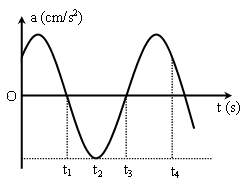
\includegraphics[width=0.4\linewidth]{../figs/C1-Q-4}
\end{center}	
	\choice
	{\True $t_1$ chất điểm bắt đầu chuyển động chậm dần}
	{$t_2$ vận tốc chất điểm cực đại}
	{$t_3$ chất điểm bắt đầu chuyển động nhanh dần}
	{$t_4$ chất điểm có thế năng tăng}
	\loigiai{Tại thời điểm $t_1$ gia tốc của chất điểm bằng 0, chất điểm chuyển động từ VTCB ra biên $\Rightarrow$ chất điểm chuyển động chậm dần.}
\end{ex}
% ===================================================================
\begin{ex}
Một vật dao động điều hoà trên trục $Ox$. Hình bên là đồ thị biểu diễn sự phụ thuộc của li độ $x$ vào thời gian $t$. Tần số $f$ của dao động là
\begin{center}
	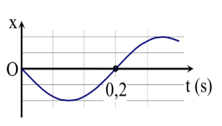
\includegraphics[width=0.3\linewidth]{../figs/C1-Q-1}
\end{center}	
	\choice
	{$\SI{10}{\radian/\second}$}
	{$\xsi{10\pi}{\radian/\second}$}
	{\True $\xsi{5\pi}{\radian/\second}$}
	{$\SI{5}{\radian/\second}$}
	\loigiai{Ta có $\dfrac{T}{2}=\SI{0.2}{\second}\Rightarrow T=\SI{0.4}{\second}$.\\
		Tần số góc của dao động:
		$$\omega=\dfrac{2\pi}{T}=\xsi{5\pi}{\radian/\second}.$$}
\end{ex}
% ===================================================================
\begin{ex}
Đồ thị biểu diễn li độ theo thời gian của một vật dao động điều hoà được thể hiện như hình bên. Biên độ dao động là
\begin{center}
	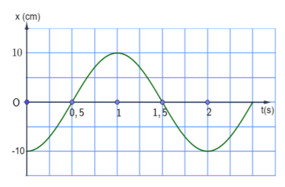
\includegraphics[width=0.4\linewidth]{../figs/C1-Q-2}
\end{center}	
	\choice
	{$\SI{5}{\centi\meter}$}
	{$\SI{-5}{\centi\meter}$}
	{\True $\SI{10}{\centi\meter}$}
	{$\SI{-10}{\centi\meter}$}
	\loigiai{}
\end{ex}
% ===================================================================
\begin{ex}
	Một chất điểm dao động điều hoà, trong 10 dao động toàn phần chất điểm đi được quãng đường $\SI{120}{\centi\meter}$. Quỹ đạo của dao động có chiều dài
	\choice
	{\True $\SI{6}{\centi\meter}$}
	{$\SI{12}{\centi\meter}$}
	{$\SI{3}{\centi\meter}$}
	{$\SI{9}{\centi\meter}$}
	\loigiai{Sau mỗi chu kì dao động chất điểm đi được quãng đường $4A$, sau 10 dao động toàn phần chất điểm đi được quãng đường 
		$$s=10\cdot4A=\SI{120}{\centi\meter}\Rightarrow A=\SI{3}{\centi\meter}$$
		Chiều dài quỹ đạo:
		$$L=2A=\SI{6}{\centi\meter}.$$}
\end{ex}
% ===================================================================
\begin{ex}
	Một vật dao động điều hoà có phương trình $x=\xsi{5\cos\left(2\pi t-\dfrac{\pi}{6}\right)}{\centi\meter}$. Lấy $\pi^2=10$. Vận tốc của vật khi có li độ $x=\SI{3}{\centi\meter}$ là
	\choice
	{$v=\SI{25.12}{\centi\meter/\second}$}
	{\True $v=\pm\SI{25.12}{\centi\meter/\second}$}
	{$v=\pm\SI{12.56}{\centi\meter/\second}$}
	{$v=\SI{12.56}{\centi\meter/\second}$}
	\loigiai{Áp dụng phương trình độc lập thời gian:
		$$x^2+\dfrac{v^2}{\omega^2}=A^2\Rightarrow v=\pm\omega\sqrt{A^2-x^2}=\pm\SI{25.12}{\centi\meter/\second}.$$}
\end{ex}
% ===================================================================
\begin{ex}
	Một con lắc lò xo gồm lò xo có độ cứng $k=\SI{40}{\newton/\meter}$ gắn với quả cầu nhỏ. Cho quả cầu dao động với biên độ $\SI{5}{\centi\meter}$. Động năng của quả cầu ở vị trí li độ $\SI{3}{\centi\meter}$ là
	\choice
	{\True $\SI{0.032}{\joule}$}
	{$\SI{320}{\joule}$}
	{$\SI{0.018}{\joule}$}
	{$\SI{180}{\joule}$}
	\loigiai{Động năng của quả cầu ở vị trí li độ $x=\SI{3}{\centi\meter}$ là
		$$W_\text{đ}=\dfrac{1}{2}k\left(A^2-x^2\right)=\SI{0.032}{\joule}.$$}
\end{ex}
% ===================================================================
\begin{ex}
Một vật dao động điều hoà có đồ thị li độ - thời gian được cho như hình bên. Lấy $\pi^2=10$. Gia tốc của vật tại thời điểm $t=\SI{1}{\second}$ là
\begin{center}
	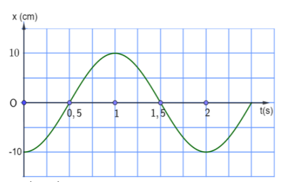
\includegraphics[width=0.4\linewidth]{../figs/C1-Q-3}
\end{center}	
	\choice
	{\True $\SI{-100}{\centi\meter/\second^2}$}
	{$\SI{100}{\centi\meter/\second^2}$}
	{$\SI{-10}{\centi\meter/\second^2}$}
	{$\SI{10}{\centi\meter/\second^2}$}
	\loigiai{Chu kì dao động:
		$$T=\SI{2}{\second}\Rightarrow \omega=\dfrac{2\pi}{T}=\xsi{\pi}{\radian/\second}$$
		Gia tốc của vật tại thời điểm $t=\SI{1}{\second}$ là:
		$$a=-\omega^2x=-\left(\xsi{\pi}{\radian/\second}\right)^2\cdot\left(\SI{10}{\centi\meter}\right)=\SI{-100}{\centi\meter/\second^2}.$$}
\end{ex}
% ===================================================================
\begin{ex}
	Một vật dao động điều hoà với phương trình $x=\xsi{5\cos\pi t}{\centi\meter}$. Tốc độ trung bình của chất điểm trong khoảng thời gian bằng $\dfrac{1}{4}$ chu kì dao động kể từ lúc $t=\SI{0}{\second}$ là
	\choice
	{$\SI{1}{\centi\meter/\second}$}
	{$\SI{2}{\centi\meter/\second}$}
	{\True $\SI{10}{\centi\meter/\second}$}
	{$\SI{20}{\centi\meter/\second}$}
	\loigiai{Chu kì dao động của vật:
		$$T=\dfrac{2\pi}{\omega}=\SI{2}{\second}.$$
		Tại thời điểm ban đầu vật đang ở vị trí biên dương, sau $\dfrac{1}{4}$ chu kì dao động vật đi được quãng đường $s=A=\SI{5}{\centi\meter}$. Tốc độ trung bình:
		$$v_\text{tb}=\dfrac{s}{t}=\dfrac{A}{\dfrac{T}{4}}=\SI{10}{\centi\meter/\second}.$$}
\end{ex}

% ===================================================================
\begin{ex}
	Hình vẽ bên là đồ thị li độ theo thời gian của một vật dao động. Phương trình dao động của vật là
	\begin{center}
		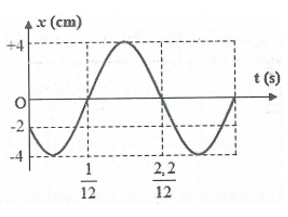
\includegraphics[width=0.4\linewidth]{../figs/C1-Q-5}
	\end{center}
	\choice
	{\True $x=\xsi{4\cos\left(10\pi t+\dfrac{2\pi}{3}\right)}{\centi\meter}$}
	{$x=\xsi{4\cos\left(20\pi t+\dfrac{2\pi}{3}\right)}{\centi\meter}$}
	{$x=\xsi{4\cos\left(10\pi t+\dfrac{5\pi}{6}\right)}{\centi\meter}$}
	{$x=\xsi{4\cos\left(20\pi t-\dfrac{\pi}{3}\right)}{\centi\meter}$}
	\loigiai{Ta có:
		\begin{align*}
			\begin{cases}
				A=\SI{4}{\centi\meter}\\
				\dfrac{T}{2}=\xsi{\dfrac{2,2-1}{12}}{\second}\Rightarrow T=\SI{0.2}{\second}\Rightarrow \omega=\dfrac{2\pi}{T}=\xsi{10\pi}{\radian/\second}
			\end{cases}
		\end{align*}
		Tại thời điểm $t=\SI{0}{\second}$ ta có 
		\begin{align*}
			\begin{cases}
				x=\SI{-2}{\centi\meter}=-\dfrac{A}{2}\\
				v<0
			\end{cases}
			\Rightarrow \varphi_0=\xsi{\dfrac{2\pi}{3}}{\radian}
		\end{align*}
		Phương trình dao động của chất điểm là $x=\xsi{4\cos\left(10\pi t+\dfrac{2\pi}{3}\right)}{\centi\meter}$.}
\end{ex}
% ===================================================================
\begin{ex}
	Một con lắc dao động tắt dần trong môi trường với lực ma sát nhỏ. Cứ sau mỗi chu kì, phần năng lượng của con lắc bị mất đi $\SI{8}{\percent}$. Trong một dao động toàn phần, biên độ giảm đi
	\choice
	{$\xsi{2\sqrt{2}}{\percent}$}
	{\True $\SI{4}{\percent}$}
	{$\SI{6}{\percent}$}
	{$\SI{1.6}{\percent}$}
	\loigiai{Năng lượng còn lại sau mỗi chu kì:
		$$W'=0,92W$$
		Biên độ dao động còn lại sau mỗi chu kì:
		$$A'=\sqrt{0,92}A=0,96A=\SI{96}{\percent}\cdot A$$
		Như vậy, sau mỗi chu kì dao động biên độ của con lắc giảm đi $\SI{4}{\percent}$.}
\end{ex}
% ===================================================================
\begin{ex}
Một con lắc lò xo có độ cứng $k=\SI{100}{\newton/\meter}$ dao động điều hoà. Gọi $W_\text{t}$, $W_\text{đ}$, $W_0$ lần lượt là thế năng, động năng và cơ năng của vật năng. Đồ thị biểu diễn sự phụ thuộc của thế năng $W_\text{t}$ và động năng $W_\text{đ}$ của con lắc vào li độ như hình vẽ. Giá trị $W_0$ là
\begin{center}
	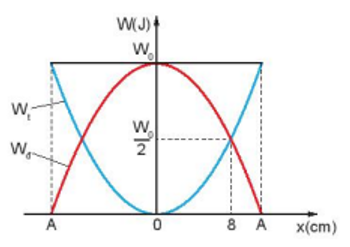
\includegraphics[width=0.4\linewidth]{../figs/C1-Q-6}
\end{center}	
	\choice
	{$\SI{0.32}{\joule}$}
	{$\SI{0.45}{\joule}$}
	{$\SI{0.96}{\joule}$}
	{\True $\SI{0.64}{\joule}$}
	\loigiai{
	Nhận thấy khi $x=\SI{8}{\centi\meter}$ thì $W_\text{t}=\dfrac{W_0}{2}$
	$$\Leftrightarrow A^2=2x^2\Rightarrow A=x\sqrt{2}=\xsi{8\sqrt{2}}{\centi\meter}$$
	Cơ năng của vật nặng:
	$$W_0=\dfrac{1}{2}kA^2=\SI{0.64}{\joule}.$$
	}
\end{ex}
% ===================================================================
\begin{ex}
Một tàu hoả chạy trên một đường ray, cứ cách khoảng $\SI{6.4}{\meter}$ trên đường ray lại có một rãnh nhỏ giữa chỗ nối các thanh ray. Chu kì dao động riêng của khung tàu trên các lò xo giảm xóc là $\SI{1.6}{\second}$. Tàu bị xóc mạnh nhất khi chạy với tốc độ bằng	
	\choice
	{$\SI{10.0}{\kilo\meter/\hour}$}
	{\True $\SI{14.4}{\kilo\meter/\hour}$}
	{$\SI{16.0}{\kilo\meter/\hour}$}
	{$\SI{20.0}{\kilo\meter/\hour}$.}
	\loigiai{Tàu bị xóc mạnh nhất khi thời gian vật đi hết đường ray bằng chu kì dao động riêng của khung tàu:
		$$v=\dfrac{\ell}{T}=\dfrac{\SI{6.4}{\meter}}{\SI{1.6}{\second}}=\SI{4}{\meter/\second}=\SI{14.4}{\kilo\meter/\hour}.$$
		}
\end{ex}
\Closesolutionfile{ans}

%	\stopcontents[mychapters]
%\stopcontents[parts]
%\fancyhf{}
%\part{ĐỀ KIỂM TRA GIỮA HỌC KÌ I}
%\chapter{Đề 1}
%\begin{center}
	ĐỀ ÔN TẬP KIỂM TRA GIỮA HỌC KỲ I – MÔN VẬT LÝ 11\\
	Thời gian làm bài: 50 phút \\
	(Không kể thời gian phát đề)\\
\end{center}
\section{Trắc nghiệm \textit{(6,0 điểm)}}
\ANSMCQ{
	\begin{center}
		\begin{tabular}{|m{2.8em}|m{2.8em}|m{2.8em}|m{2.8em}|m{2.8em}|m{2.8em}|m{2.8em}|m{2.8em}|m{2.8em}|m{2.8em}|}
			\hline
			1D & 2A & 3C & 4A & 5B & 6D & 7A & 8A & 9C & 10A\\
			\hline
			11C & 12B & 13C & 14D & 15A & 16B & 17B & 18A & 19C & 20C\\
			\hline
		\end{tabular}
	\end{center}}

\begin{enumerate}[label=\bfseries Câu \arabic*:]
	\item Chuyển động của vật nào dưới đây không phải là dao động cơ?
	\begin{mcq}
		\item Chuyển động của pittong trong xilanh khi động cơ hoạt động.
		\item Chuyển động của con lắc đồng hồ gắn trong đồng hồ quả lắc.
		\item Chuyển động của chiếc lá nổi trên mặt nước khi có sóng truyền qua.
		\item Chuyển động của một vật trượt trên mặt phẳng nghiêng.
	\end{mcq}
\hideall{
\textbf{Đáp án D.}\\
Dao động cơ là sự chuyển động qua lại của một vật quanh vị trí cân bằng. Sự chuyển động của một vật trượt trên mặt phẳng nghiêng không phải là dao động cơ.
}

\item Biên độ dao động là 
\begin{mcq}
	\item độ dịch chuyển cực đại của vật tính từ vị trí cân bằng.
	\item độ dịch chuyển cực tiểu của vật tính từ vị trí cân bằng.
	\item độ dịch chuyển cực đại của vật tính từ vị trí biên.
	\item độ dịch chuyển cực tiểu của vật tính từ vị trí biên.
\end{mcq}
\hideall{
\textbf{Đáp án A.}
}

\item 
{Hình bên là đồ thị toạ độ theo thời gian của ba chuyển động. Chuyển động ứng với đồ thị nào là dao động điều hoà 
	\begin{center}
		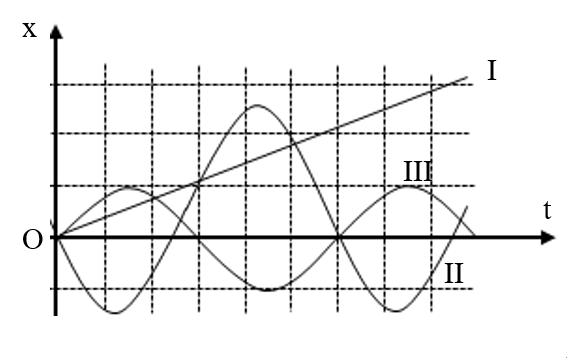
\includegraphics[width=0.4\linewidth]{../figs/D11-1-1}
\end{center}}
{\begin{mcq}(2)
		\item Đồ thị I.
		\item Đồ thị II.
		\item Đồ thị III.
		\item Đồ thị II và III.
\end{mcq}}
{\hideall{
		\textbf{Đáp án C.}
}}

\item Một vật nhỏ dao động điều hoà theo một trục cố định. Đồ thị li độ của vật theo thời gian có dạng 
\begin{mcq}(4)
	\item hình sin.	
	\item đường tròn.
	\item đường thẳng. 
	\item đường elip.
\end{mcq}
\hideall{
\textbf{Đáp án A.}
}

\item Công thức tính chu kì dao động của con lắc lò xo là
\begin{mcq}(4)
	\item $T=2\pi\sqrt{\dfrac{k}{m}}$.
	\item $T=2\pi\sqrt{\dfrac{m}{k}}$.
	\item $T=\dfrac{\pi}{2}\sqrt{\dfrac{m}{k}}$.
	\item $T=\sqrt{\dfrac{k}{m}}$.
\end{mcq}
\hideall{
\textbf{Đáp án B.}
}

\item Một vật nặng có khối lượng $m$, dao động điều hoà với phương trình $x=A\cos\omega t$. Cơ năng của vật là
\begin{mcq}(4)
	\item $m\omega A^2$.
	\item $\dfrac{1}{2}m\omega A^2$.
	\item $m\omega^2A^2$.
	\item $\dfrac{1}{2}m\omega^2A^2$.
\end{mcq}
\hideall{
\textbf{Đáp án D.}\\
Cơ năng của vật dao động điều hoà $W=\dfrac{1}{2}\omega^2A^2$.
}

\item Một con lắc đơn gồm vật nặng có khối lượng $m$, dây treo có chiều dài $\ell$ đang dao động tại nơi có gia tốc trọng trường $g$. Thế năng của con lắc ở li độ góc $\alpha$ là
\begin{mcq}(2)
	\item $W_t=mg\ell\left(1-\cos\alpha\right).$
	\item $W_t=mg\ell\left(1-\sin\alpha\right).$
	\item $W_t=mg\ell\cos\alpha.$
	\item $W_t=mg\ell\sin\alpha.$
\end{mcq}
\hideall{
\textbf{Đáp án A.}\\
}

\item Một vật dao động điều hòa đang chuyển động từ vị trí biên về vị trí cân bằng. Nhận xét nào sau đây là đúng?
\begin{mcq}
	\item Năng lượng của vật đang chuyển hóa từ thế năng sang động năng.
	\item Thế năng tăng dần và động năng giảm dần.
	\item Cơ năng của vật tăng dần đến giá trị lớn nhất.
	\item Thế năng của vật tăng dần nhưng cơ năng của vật không đổi.
\end{mcq}
\hideall{
\textbf{Đáp án A.}
}
\item Mỗi khi xe buýt đến bến, xe chỉ tạm dừng nên không tắt máy. Hành khách trên xe nhận thấy thân xe dao động, dao động này là
\begin{mcq}(2)
	\item dao động tắt dần.
	\item dao động duy trì.
	\item dao động cưỡng bức.
	\item dao động riêng.
\end{mcq}
\hideall{
\textbf{Đáp án C.}
}

\item Dao động tắt dần là dao động
\begin{mcq}(2)
\item có biên độ giảm dần theo thời gian. 
\item có chu kì giảm dần theo thời gian.
\item có động năng giảm dần theo thời gian.	
\item có tần số giảm dần theo thời gian.
\end{mcq}
\hideall{
\textbf{Đáp án A.}
}

\item Tác hại nào sau đây gây ra \textbf{không phải} do cộng hưởng?
\begin{mcq}
	\item Máy đầm hoạt động có thể gây ra rung lắc, nứt tường nhà.
	\item Động cơ ô tô hoạt động có thể gây rung lắc khung xe rất mạnh.
	\item Xe dao động mạnh khi qua “ổ gà” nên phải chế tạo bộ phận giảm xóc.
	\item Âm thanh quá lớn có thể làm chảy máu tai.
\end{mcq}
\hideall{
\textbf{Đáp án C.}
}

\item Một con lắc đơn dao động điều hoà thực hiện 10 dao động toàn phần trong thời gian $\SI{16}{\second}$. Biết gia tốc trọng trường $g=\xsi{\pi^2}{\meter/\second^2}$, chiều dài con lắc là
\begin{mcq}(4)
	\item $\SI{0.9}{\meter}$.
	\item $\SI{0.64}{\meter}$.
	\item $\SI{0.81}{\meter}$.
	\item $\SI{1.8}{\meter}$.
\end{mcq}
\hideall{
\textbf{Đáp án B.}\\
$$T=\dfrac{t}{N}=2\pi\sqrt{\dfrac{\ell}{g}}\Rightarrow \ell=\SI{0.64}{\meter}.$$
}

\item Một vật dao động điều hoà với phương trình $x=\xsi{4\cos\left(4\pi t-\dfrac{\pi}{4}\right)}{\centi\meter}$. Chu kì dao động của vật là
\begin{mcq}(4)
	\item $\xsi{4\pi}{\second}$.
	\item $\SI{2}{\second}$.
	\item $\SI{0.5}{\second}$.
	\item $\xsi{2\pi}{\second}$.
\end{mcq}
\hideall{
\textbf{Đáp án C.}
Chu kì dao động của vật:
$$T=\dfrac{2\pi}{\omega}=\SI{0.5}{\second}.$$
}

\item {Một vật dao động điều hoà có đồ thị li độ - thời gian được mô tả như hình bên. Gia tốc của vật dao động tại thời điểm $t=\SI{3}{\second}$ là
	\begin{center}
		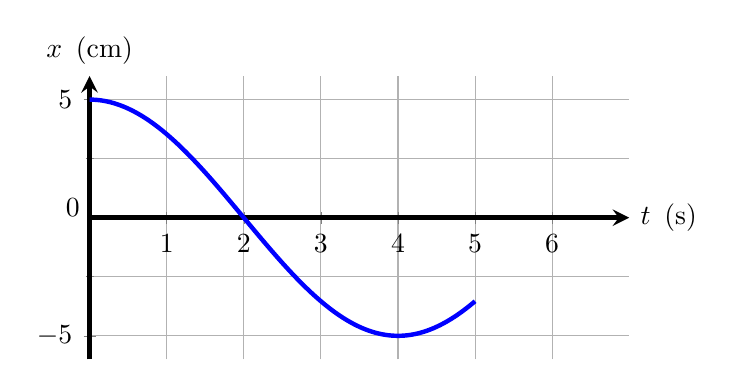
\begin{tikzpicture}  
			\begin{axis}[  ultra thick,
				xmin=0,  
				xmax=7,  
				xtick={0,1,...,6},
				ytick={-5,0,5},
				minor x tick num=0,
				minor y tick num=1,
				ymin=-6,  
				ymax=6, 
				y=0.3cm,
				samples=300,
				axis lines=center, 
				grid style={step=1, color=gray!60!white},
				grid=both,
				xlabel=$t\ \left(\si{\second}\right)$, 
				ylabel=$x\ \left(\si{\centi\meter}\right)$, 
				every axis y label/.style={at=(current axis.above origin),anchor=south},  
				every axis x label/.style={at=(current axis.right of origin),anchor=west},  ]
				\addplot [ultra thick, blue, smooth, domain=0:5] {5*cos(deg(pi*x/4))}; 
			\end{axis}  
			\node[label={[left]90:0}] at (0,1.8){};
		\end{tikzpicture}
	\end{center}
	
\begin{mcq}(4)
	\item $\SI{2.77}{\centi\meter/\second^2}$.
	\item $\SI{-2.18}{\centi\meter/\second^2}$.
	\item $\SI{-2.77}{\centi\meter/\second^2}$.
	\item $\SI{2.18}{\centi\meter/\second^2}$.
\end{mcq}}
\hideall{
\textbf{Đáp án D.}\\
Chu kì dao động của vật
$$T=\SI{8}{\second}\Rightarrow \omega=\dfrac{2\pi}{T}=\xsi{\dfrac{\pi}{4}}{\radian/\second}$$
Phương trình li độ của vật:
$$x=\xsi{5\cos\left(\dfrac{\pi}{4}t\right)}{\centi\meter}$$
Tại thời điểm $t=\SI{3}{\second}$ thì $x=\xsi{\dfrac{5\sqrt{2}}{2}}{\centi\meter}$.\\
Gia tốc của vật lúc này:
$$a=-\omega^2x=\SI{2.18}{\centi\meter/\second^2}.$$
}

\item Một vật dao động điều hoà có vận tốc cực đại là $v_\text{max}=\xsi{8\pi}{\centi\meter/\second}$ và gia tốc cực đại là $a_\text{max}=\xsi{16\pi^2}{\centi\meter/\second^2}$. Tần số góc của dao động là
\begin{mcq}(4)
	\item $\xsi{2\pi}{\radian/\second}$.
	\item $\xsi{4\pi}{\radian/\second}$.
	\item $\xsi{2\pi^2}{\radian/\second}$.
	\item $\xsi{4\pi^2}{\radian/\second}$.
\end{mcq}
\hideall{
\textbf{Đáp án A.}\\
Ta có:
\begin{align*}
	\begin{cases}
		a_\text{max}=\omega^2A\\
		v_\text{max}=\omega A
	\end{cases}
\Rightarrow \omega=\dfrac{a_\text{max}}{v_\text{max}}=\xsi{2\pi}{\radian/\second}
\end{align*}
}

\item Một vật dao động điều hoà với biên độ $A$ và cơ năng $W$. Mốc thế năng của vật ở vị trí cân bằng. Khi vật đi qua vị trí có li độ $\dfrac{2}{3}A$ thì động năng của vật là
\begin{mcq}(4)
	\item $\dfrac{7}{9}W$.
	\item $\dfrac{5}{9}W$.
	\item $\dfrac{4}{9}W$.
	\item $\dfrac{2}{9}W$.
\end{mcq}
\hideall{
	\textbf{Đáp án B.}\\
	Khi vật qua vị trí $x=\dfrac{2}{3}A$ thì 
$$\dfrac{W_t}{W}=\dfrac{x^2}{A^2}=\dfrac{4}{9}\Rightarrow W_t=\dfrac{4}{9}W\Rightarrow W_\text{đ}=W-W_\text{t}=\dfrac{5}{9}W.$$
}


\item 
{Đồ thị biểu diễn li độ theo thời gian của một vật dao động điều hoà được mô tả như hình bên. Pha ban đầu của dao động là
\begin{center}
	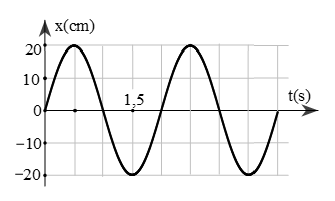
\includegraphics[width=0.4\linewidth]{../figs/D11-1-2}
\end{center}}
{\begin{mcq}(4)
	\item $\xsi{\dfrac{\pi}{2}}{\radian}$.
	\item $\xsi{-\dfrac{\pi}{2}}{\radian}$.
	\item $\xsi{\pi}{\radian}$.
	\item $\xsi{-\pi}{\radian}$.
	\end{mcq}}
{\hideall{
		\textbf{Đáp án B.}
	}}

\item Một chất điểm dao động điều hoà với phương trình vận tốc $v=\xsi{2\sqrt{2}\cos\left(2t+\dfrac{5\pi}{6}\right)}{\centi\meter/\second}$. Tại thời điểm vật có vận tốc tức thời $\SI{2}{\centi\meter/\second}$ thì li độ của vật có thể là
\begin{mcq}(4)
	\item $\SI{1}{\centi\meter}$.
	\item $\xsi{\sqrt{2}}{\centi\meter}$.
	\item $\SI{2}{\centi\meter}$.
	\item $\xsi{2\sqrt{2}}{\centi\meter}$.
\end{mcq}
\hideall{
\textbf{Đáp án A.}\\
Biên độ dao động:
$$A=\dfrac{v_\text{max}}{\omega}=\xsi{\sqrt{2}}{\centi\meter}$$
Áp dụng hệ thức độc lập thời gian:
$$\left(\dfrac{v}{v_\text{max}}\right)^2+\left(\dfrac{x}{A}\right)^2=1\Rightarrow x^2=A^2\left[1-\left(\dfrac{v}{v_\text{max}}\right)^2\right]=\pm\SI{1}{\centi\meter}.$$
}

\item 
{Cho một chất điểm dao động điều hoà quanh vị trí cân bằng O. Li độ biến thiên theo thời gian như mô tả trong đồ thị hình bên. Kẻ đường tiếp tuyến với đồ thị li độ ở thời điểm $t=\SI{0.75}{\second}$ thì thấy nó cắt trục $Ot$ ở giá trị $\SI{0.43}{\second}$. Vận tốc của chất điểm ở thời điểm đó gần với giá trị nào sau đây nhất?
\begin{center}
	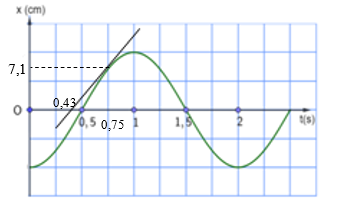
\includegraphics[width=0.4\linewidth]{../figs/D11-1-3}
\end{center}
\begin{mcq}(4)
	\item $\SI{8.1}{\centi\meter/\second}.$
	\item $\SI{-8.1}{\centi\meter/\second}.$
	\item $\SI{22.2}{\centi\meter/\second}.$
	\item $\SI{-22.2}{\centi\meter/\second}.$
\end{mcq}
}
{
\hideall{
\textbf{Đáp án C.}\\
Vận tốc tức thời của vật tại một thời điểm được xác định bằng độ dốc tiếp tuyến đồ thị $x-t$:
$$v=\tan\alpha=\dfrac{\Delta x}{\Delta t}=\dfrac{\SI{7.1}{\centi\meter}-\SI{0}{\centi\meter}}{\SI{0.75}{\second}-\SI{0.43}{\second}}\approx\SI{22.19}{\centi\meter/\second}.$$
}
}

\item 
{Chất điểm khối lượng $\SI{200}{\gram}$ dao động điều hoà quanh vị trí cân bằng O. Li độ của chất điểm biến thiên theo thời gian như đồ thị hình bên. Cơ năng của chất điểm trong quá trình dao động là
	\begin{center}
		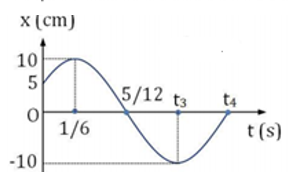
\includegraphics[width=0.35\linewidth]{../figs/D11-1-4}
	\end{center}
\begin{mcq}(4)
	\item $\SI{0.1}{\joule}$.
	\item $\SI{0.05}{\joule}$.
	\item $\SI{0.04}{\joule}$.
	\item $\SI{0.01}{\joule}$.
\end{mcq}
}
\hideall{
\textbf{Đáp án C.}\\
Biên độ dao động của chất điểm $A=\SI{10}{\centi\meter}=\SI{0.1}{\meter}$.
Chu kì dao động của chất điểm:
$$\dfrac{T}{4}=\xsi{\dfrac{5}{12}}{\second}-\xsi{\dfrac{1}{6}}{\second}=\xsi{0.25}{\second}\Rightarrow T=\SI{1}{\second}$$
Cơ năng của chất điểm trong quá trình dao động:
$$W=\dfrac{1}{2}m\omega^2A^2=\dfrac{1}{2}\cdot\left(\SI{0.2}{\kilogram}\right)\cdot\left(\dfrac{2\pi}{\SI{1}{\second}}\right)^2\cdot\left(\SI{0.1}{\meter}\right)^2\approx\SI{0.04}{\joule}.$$

}
\end{enumerate}
\section{Tự luận \textit{(4,0 điểm)}}
\begin{enumerate}[label=\bfseries Bài \arabic*:]
	\item Xét một con lắc lò xo đang dao động điều hoà với đồ thị gia tốc - thời gian như hình bên. Với lò xo được sử dụng có độ cứng $k=\SI{500}{\newton/\meter}$ và lấy $\pi^2=10$. Hãy xác định:
	\begin{center}
		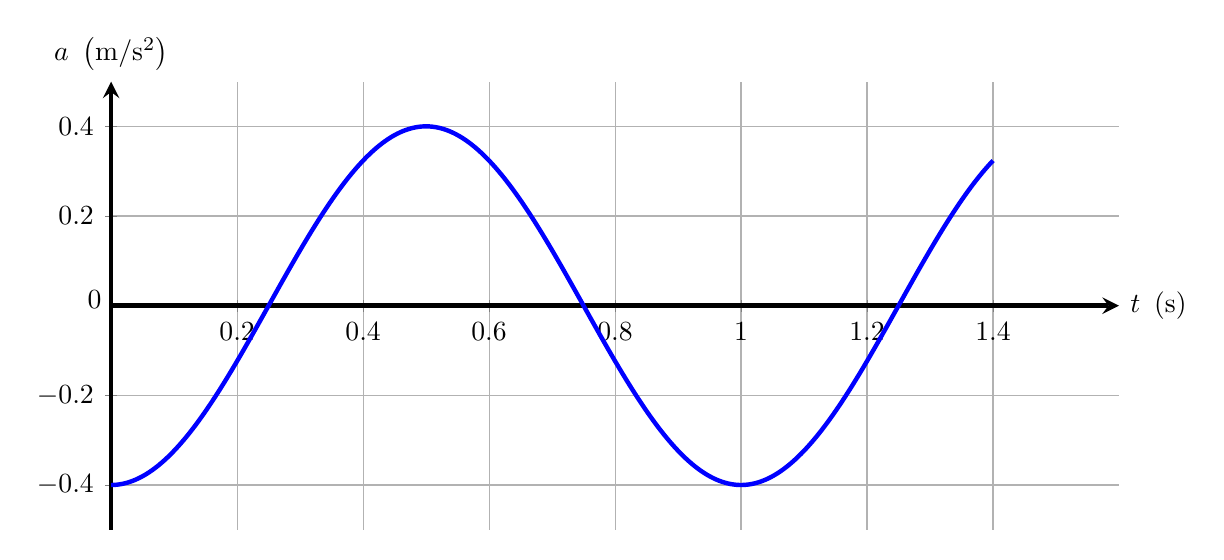
\begin{tikzpicture}  
			\begin{axis}[  ultra thick,
				xmin=0,  
				xmax=1.6,  
				xtick={0,0.2,...,1.4},
				ytick={-0.4,-0.2,...,0.4},
				minor x tick num=0,
				minor y tick num=0,
				ymin=-0.5,  
				ymax=0.5, 
				x=8cm,
				samples=300,
				axis lines=center, 
				grid style={step=0, color=gray!60!white},
				grid=both,
				xlabel=$t\ \left(\si{\second}\right)$, 
				ylabel=$a\ \left(\si{\meter/\second^2}\right)$, 
				every axis y label/.style={at=(current axis.above origin),anchor=south},  
				every axis x label/.style={at=(current axis.right of origin),anchor=west},  ]
				\addplot [ultra thick, blue, smooth, domain=0:1.4] {0.4*cos(deg(pi*x*2+pi))}; 
			\end{axis}  
			\node[label={[left]90:0}] at (0,2.8){};
		\end{tikzpicture}
	\end{center}
	\begin{enumerate}[label=\alph*)]
		\item Khối lượng của vật nặng.
		\item Li độ của vật tại thời điểm $t=\SI{1.4}{\second}$.
	\end{enumerate}
\hideall{
\begin{enumerate}[label=\alph*)]
	\item Dựa vào đồ thị, ta có: $T=\SI{1}{\second}\Rightarrow \omega=\dfrac{2\pi}{T}=\xsi{2\pi}{\radian/\second}$.\\
	Khối lượng của vật nặng:
	$$m=\dfrac{k}{\omega^2}=\dfrac{\SI{500}{\newton/\meter}}{\left(\xsi{2\pi}{\radian/\second}\right)^2}=\SI{12.5}{\kilogram}.$$
	\item Dựa vào đồ thị, ta có:
	$$a_\text{max}=\SI{0.4}{\meter/\second^2}\Rightarrow A=\dfrac{a_\text{max}}{\omega^2}=\dfrac{\SI{0.4}{\meter/\second^2}}{\left(\xsi{2\pi}{\radian/\second}\right)^2}=\SI{0.01}{\meter}=\SI{1}{\centi\meter}.$$
	Tại thời điểm ban đầu, gia tốc có giá trị cực tiểu nên vật ở vị trí biên dương, suy ra pha ban đầu của dao động là $\SI{0}{\radian}$.\\
	Phương trình li độ của vật dao động: 
	$$x=\xsi{\cos\left(2\pi t\right)}{\centi\meter}$$
	Li độ của vật tại thời điểm $t=\SI{1.4}{\second}$ là:
	$$x=\cos\left[\left(\xsi{2\pi}{\radian/\second}\right)\cdot\left(\SI{1.4}{\second}\right)\right]\approx\SI{-0.84}{\centi\meter}.$$
\end{enumerate}
}

\item Cho một dao động tắt dần, nếu xem gần đúng dao động tắt dần này là dao động điều hoà, cứ sau mỗi chu kì thì cơ năng của hệ sẽ giảm $\SI{24}{\percent}$. Hỏi sau khoảng bao nhiêu chu kì, biên độ của dao động sẽ giảm còn một nửa?
\hideall{
Cơ năng ban đầu của dao động 
$$W=\dfrac{1}{2}m\omega^2A^2$$
Cơ năng của dao động sau mỗi chu kì còn lại là $W'=0,76W$. Do đó, biên độ của dao động sau mỗi chu kì là $A_1=\sqrt{0,76}A_0$.\\
Vậy sau $N$ chu kì thì biên độ dao động còn lại là $A_N=\left(\sqrt{0,76}\right)^NA_0$.\\
Khi $A_N=\dfrac{1}{2}A_0$, ta thu được $N\approx5$.\\
Vậy sau khoảng 5 chu kì dao động thì biên độ dao động giảm còn 1 nửa.
}
\end{enumerate}
%\chapter{Đề 2}
%\begin{center}
	ĐỀ ÔN TẬP KIỂM TRA GIỮA HỌC KỲ I – MÔN VẬT LÝ 11\\
	Thời gian làm bài: 50 phút \\
	(Không kể thời gian phát đề)\\
\end{center}
\section{Trắc nghiệm \textit{(6,0 điểm)}}
\ANSMCQ{
	\begin{center}
		\begin{tabular}{|m{2.8em}|m{2.8em}|m{2.8em}|m{2.8em}|m{2.8em}|m{2.8em}|m{2.8em}|m{2.8em}|m{2.8em}|m{2.8em}|}
			\hline
			1D & 2A & 3B & 4A & 5C & 6A & 7D & 8B & 9C & 10B\\
			\hline
			11D & 12B & 13D & 14C & 15A & 16A & 17C & 18A & 19B & 20D\\
			\hline
		\end{tabular}
\end{center}}
\begin{enumerate}[label=\bfseries Câu \arabic*:]
	\item Khi vật thực hiện một dao động tương ứng với pha dao động sẽ thay đổi một lượng 
	\begin{mcq}(4)
		\item $\SI{0}{\radian}$.
		\item $\xsi{\dfrac{\pi}{2}}{\radian}$.
		\item $\xsi{\pi}{\radian}$.
		\item $\xsi{2\pi}{\radian}$.
	\end{mcq}
\hideall{
\textbf{Đáp án D.}
}


\item Đơn vị đo của tần số dao động trong hệ đơn vị SI là 
\begin{mcq}(4)
	\item $\si{\hertz}$.
	\item $\si{\second}$.
	\item $\si{\centi\meter}$.
	\item $\si{\meter}$.
\end{mcq}
\hideall{
\textbf{Đáp án A.}
}

\item Độ dịch chuyển cực đại của vật tính từ vị trí cân bằng gọi là
\begin{mcq}(4)
	\item li độ dao động.
	\item biên độ dao động.
	\item tần số góc.
	\item pha ban đầu.
\end{mcq}
\hideall{
\textbf{Đáp án B.}
}

\item Trong các dao động được mô tả dưới đây, dao động nào được xem là dao động tuần hoàn? 
\begin{mcq}
	\item Dao động của con lắc đồng hồ khi đang hoạt động. 
	\item Dao động của chiếc thuyền trên mặt sông. 
	\item Dao động của quả bóng cao su đang nảy trên mặt đất. 
	\item Dao động của dây đàn sau khi được gảy.
\end{mcq}
\hideall{
\textbf{Đáp án A.}\\
Dao động tuần hoàn là dao động mà trạng thái chuyển động được lặp lại như cũ sau những khoảng thời gian bằng nhau xác định.
}

\item Một vật dao động điều hoà trên trục $Ox$. Hình bên là đồ thị biểu diễn sự phụ thuộc của li độ $x$ vào thời gian $t$. Tần số góc của dao động là
\begin{center}
	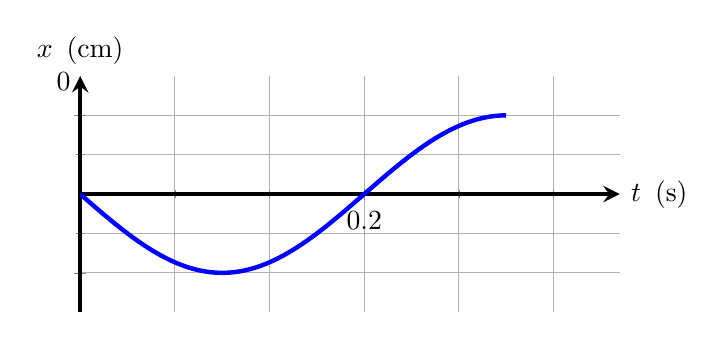
\begin{tikzpicture}  
		\begin{axis}[  ultra thick,
			xmin=0,  
			xmax=0.38,  
			xtick={0,0.2,0.4},
			ytick={-2,0,2},
			minor x tick num=2,
			minor y tick num=1,
			ymin=-3,  
			ymax=3, 
			y=0.5cm,
			samples=300,
			yticklabels=\empty,
			axis lines=center, 
			grid style={step=1, color=gray!60!white},
			grid=both,
			xlabel=$t\ \left(\si{\second}\right)$, 
			ylabel=$x\ \left(\si{\centi\meter}\right)$, 
			every axis y label/.style={at=(current axis.above origin),anchor=south},  
			every axis x label/.style={at=(current axis.right of origin),anchor=west},  ]
			\addplot [ultra thick, blue, smooth, domain=0:0.3] {2*cos(deg(5*pi*x+pi/2))}; 
		\end{axis}  
		\node[label={[left]90:0}] at (0,2.8){};
	\end{tikzpicture}
\end{center}
\begin{mcq}(4)
	\item $\SI{10}{\radian/\second}$.
	\item $\xsi{10\pi}{\radian/\second}$.
	\item $\xsi{5\pi}{\radian/\second}$.
	\item $\SI{5}{\radian/\second}$.
\end{mcq}
\hideall{
\textbf{Đáp án C.}\\
Chu kì dao động của vật $T=\SI{0.4}{\second}$.\\
Tần số góc dao động:
$$\omega=\dfrac{2\pi}{T}=\xsi{5\pi}{\radian/\second}.$$
}

\item Các nhà thực nghiệm đo được tần số dao động của một hệ gồm thanh silicon siêu nhỏ có virus dính trên đó đang thực hiện dao động là $\SI{2.87E14}{\hertz}$. Tần số góc của hệ dao động trên bằng bao nhiêu? 
\begin{mcq}(4)
	\item $\SI{1.80E15}{\radian/\second}$.
	\item $\SI{3.48E15}{\radian/\second}$.
	\item $\SI{2.18E14}{\radian/\second}$.
	\item $\SI{4.57E14}{\radian/\second}$.
\end{mcq}
\hideall{
\textbf{Đáp án A.}\\
Tần số góc của dao động:
$$\omega=2\pi f=\SI{1.80E15}{\radian/\second}.$$
}

\item Một vật dao động điều hoà trên trục $Ox$. Vận tốc của vật
\begin{mcq}(2)
	\item luôn có giá trị không đổi.
	\item luôn có giá trị dương.
	\item là hàm bậc hai của thời gian.
	\item biến thiên điều hoà theo thời gian.
\end{mcq}
\hideall{
\textbf{Đáp án D.}\\
Vận tốc của vật dao động điều hoà biến thiên điều hoà theo thời gian.
}

\item Khi nói về dao động điều hòa của một vật, phát biểu nào sau đây đúng?
\begin{mcq}
	\item Khi vật ở vị trí biên, gia tốc của vật bằng không.
	\item Vectơ gia tốc của vật luôn hướng về vị trí cân bằng.
	\item Vectơ vận tốc của vật luôn hướng về vị trí cân bằng.
	\item Khi đi qua vị trí cân bằng, vận tốc của vật bằng không.
\end{mcq}
\hideall{
\textbf{Đáp án B.}
}

\item Khi tiến hành thí nghiệm khảo sát vị trí vật nặng của con lắc lò xo đang dao động bằng cách sử dụng thước thẳng, bạn học sinh thấy rằng vật nặng dao động từ vị trí $\SI{1}{\centi\meter}$ đến vị trí $\SI{11}{\centi\meter}$ trên thước. Biên độ dao động của vật nặng trong con lắc lò xo là 
\begin{mcq}(4)
	\item $\SI{10}{\centi\meter}$.
	\item $\SI{6}{\centi\meter}$.
	\item $\SI{5}{\centi\meter}$.
	\item $\SI{12}{\centi\meter}$.
\end{mcq}
\hideall{
\textbf{Đáp án C.}\\
Biên độ dao động của vật nặng trong con lắc lò xo:
$$A=\dfrac{\ell_\text{max}-\ell_\text{min}}{2}=\SI{5}{\centi\meter}.$$
}

\item Trong dao động điều hoà, khoảng thời gian mà vật thực hiện được 1 dao động toàn phần gọi là
\begin{mcq}(4)
	\item biên độ,
	\item chu kì.
	\item tần số.
	\item pha ban đầu.
\end{mcq}
\hideall{
\textbf{Đáp án B.}\\
Khoảng thời gian mà vật thực hiện được 1 dao động toàn phần gọi là chu kì dao động.
}

\item Một bạn học sinh quan sát thấy con lắc trong đồng hồ quả lắc thực hiện được 20 dao động trong 30 giây. Dao động của con lắc trong đồng hồ này có đặc điểm nào sau đây? 
\begin{mcq}(2)
	\item Dao động điều hoà, tần số là $\SI{1.5}{\hertz}$.
	\item Dao động điều hoà, tần số là $\SI{0.7}{\hertz}$.
	\item Dao động tuần hoàn, tần số là $\SI{1.5}{\hertz}$.
	\item Dao động tuần hoàn, tần số là $\SI{0.7}{\hertz}$.
\end{mcq}
\hideall{
\textbf{Đáp án D.}\\
Dao động của con lắc đồng hồ là dao động tuần hoàn với tần số
$$f=\dfrac{N}{\Delta t}=\dfrac{20}{\SI{30}{\second}}\approx\SI{0.67}{\hertz}.$$
}

\item Hai vật dao động điều hoà có đồ thị li độ - thời gian như hình vẽ. Phát biểu nào sau đây mô tả đúng tính chất của hai vật?
\begin{center}
	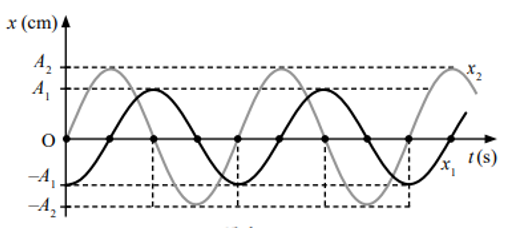
\includegraphics[width=0.6\linewidth]{../figs/D11-2-1}
\end{center}
\begin{mcq}(2)
	\item Hai vật dao động cùng tần số, cùng pha. 
	\item Hai vật dao động cùng tần số, vuông pha. 
	\item Hai vật dao động khác tần số, cùng pha. 
	\item Hai vật dao động khác tần số, vuông pha.
\end{mcq}
\hideall{
\textbf{Đáp án B.}\\
Dựa vào đồ thị li độ - thời gian, ta nhận thấy hai vật dao động cùng tần số.\\
Tại thời điểm $t=0$, vật 2 qua VTCB theo chiều dương. Sau khoảng thời gian $\Delta t=\dfrac{T}{4}$ vật 1 có cùng trạng thái dao động với vật 2 ở thời điểm $t=0$. Suy ra, độ lệch pha giữa hai dao động:
$$\Delta \varphi=\dfrac{\Delta t}{T}\cdot2\pi=\xsi{\dfrac{\pi}{2}}{\radian}.$$
}

\item Đồ thị li độ thời gian của một vật dao động điều hoà được thể hiện như hình vẽ. Phương trình dao động của vật là
\begin{center}
	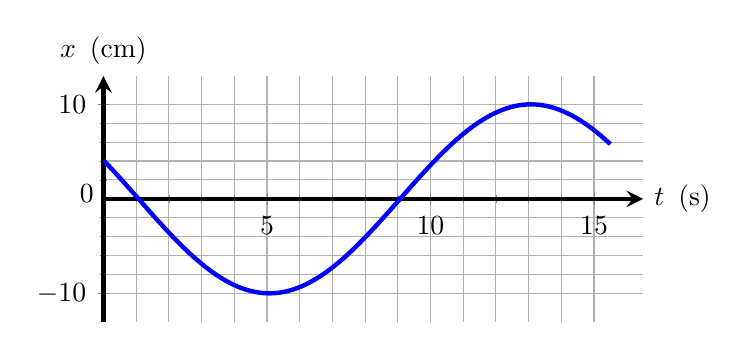
\begin{tikzpicture}  
		\begin{axis}[  ultra thick,
			xmin=0,  
			xmax=16.5,  
			xtick={0,5,10,15},
			ytick={-10,0,10},
			minor x tick num=4,
			minor y tick num=4,
			ymin=-13,  
			ymax=13, 
			y=0.12cm,
			samples=300,
			axis lines=center, 
			grid style={step=1, color=gray!60!white},
			grid=both,
			xlabel=$t\ \left(\si{\second}\right)$, 
			ylabel=$x\ \left(\si{\centi\meter}\right)$, 
			every axis y label/.style={at=(current axis.above origin),anchor=south},  
			every axis x label/.style={at=(current axis.right of origin),anchor=west},  ]
			\addplot [ultra thick, blue, smooth, domain=0:15.5] {10*cos(deg(pi*x/8+1.15))}; 
		\end{axis}  
		\node[label={[left]90:0}] at (0,1.5){};
	\end{tikzpicture}
\end{center}
	\begin{mcq}(2)
		\item $x=\xsi{10\cos\left(16t+1,37\right)}{\centi\meter}$.
		\item $x=\xsi{10\cos\left(\dfrac{\pi}{8}t-1,18\right)}{\centi\meter}$.
		\item $x=\xsi{10\cos\left(16t-1,37\right)}{\centi\meter}$.
		\item $x=\xsi{10\cos\left(\dfrac{\pi}{8}t+1,18\right)}{\centi\meter}$.
	\end{mcq}
\hideall{
\textbf{Đáp án D.}\\
Chu kì dao động của vật:
$$\dfrac{T}{2}=\SI{13}{\second}-\SI{5}{\second}\Rightarrow T=\SI{16}{\second}$$
Tần số góc dao động:
$$\omega=\dfrac{2\pi}{T}=\xsi{\dfrac{\pi}{8}}{\radian/\second}$$
Tại thời điểm $t=\SI{5}{\second}$, vật đang ở vị trí biên âm, pha dao động của vật lúc này
$$\varphi=\omega t+\varphi_0=\xsi{\pi}{\radian}\Rightarrow \varphi_0=\varphi-\omega t=\xsi{\pi}{\radian}-\left(\xsi{\dfrac{\pi}{8}}{\radian/\second}\right)\cdot\left(\SI{5}{\second}\right)=\xsi{\dfrac{3\pi}{8}}{\radian}\approx\SI{1.18}{\radian}.$$
Phương trình dao động của vật:
$$x=\xsi{10\cos\left(\dfrac{\pi}{8}t+1,18\right)}{\centi\meter}.$$
}

\item Một vật dao động điều hoà với chu kì $\SI{2}{\second}$, biên độ $\SI{10}{\centi\meter}$. Khi vật cách vị trí biên $\SI{4}{\centi\meter}$ thì tốc độ của nó bằng
\begin{mcq}(4)
	\item $\SI{18.33}{\centi\meter/\second}$.
	\item $\SI{28.79}{\centi\meter/\second}$.
	\item $\SI{25.13}{\centi\meter/\second}$.
	\item $\SI{18.84}{\centi\meter/\second}$.
\end{mcq}
\hideall{
\textbf{Đáp án C.}\\
Tốc độ của vật khi cách vị trí biên $\SI{4}{\centi\meter}$ $\left(\left|x\right|=\SI{6}{\centi\meter}\right)$:
$$\left|v\right|=\omega\sqrt{A^2-x^2}=\left(\dfrac{\xsi{2\pi}{\radian}}{\SI{2}{\second}}\right)\sqrt{\left(\SI{10}{\centi\meter}\right)^2-\left(\SI{6}{\centi\meter}\right)^2}\approx\SI{25.13}{\centi\meter/\second}.$$
}

\item Một vật dao động điều hoà có gia tốc biến đổi theo thời gian $a=\xsi{8\cos\left(20t-\dfrac{\pi}{2}\right)}{\centi\meter/\second^2}$. Phương trình dao động của vật là
\begin{mcq}(2)
	\item $x=\xsi{0,02\cos\left(20t+\dfrac{\pi}{2}\right)}{\centi\meter}.$
	\item $x=\xsi{2\cos\left(20t-\dfrac{\pi}{2}\right)}{\centi\meter}.$
	\item $x=\xsi{4\cos\left(20t+\dfrac{\pi}{2}\right)}{\centi\meter}.$
	\item $x=\xsi{2\cos\left(20t+\dfrac{\pi}{2}\right)}{\centi\meter}.$
\end{mcq}
\hideall{
\textbf{Đáp án A.}\\
Biên độ dao động của vật:
$$A=\dfrac{a_\text{max}}{\omega^2}=\dfrac{\SI{8}{\centi\meter/\second^2}}{\left(\SI{20}{\radian/\second}\right)^2}=\SI{0.02}{\centi\meter}$$
Pha ban đầu của dao động:
$$\varphi_{0x}=\varphi_{0a}+\pi=\xsi{\dfrac{\pi}{2}}{\radian}.$$
Vậy phương trình dao động của vật $x=\xsi{0,02\cos\left(20t+\dfrac{\pi}{2}\right)}{\centi\meter}$.\\
}

\item Một chất điểm dao động điều hoà, gia tốc $a$ và li độ $x$ của chất điểm liên hệ với nhau bởi hệ thức $a=-4\pi^2x$, trong đó $a$ có đơn vị $\si{\centi\meter/\second^2}$; $x$ có đơn vị $\si{\centi\meter}$. Chu kì dao động bằng
\begin{mcq}(4)
	\item $\SI{1}{\second}$.
	\item $\SI{0.25}{\second}$.
	\item $\SI{0.5}{\second}$.
	\item $\SI{0.4}{\second}$.
\end{mcq}
\hideall{
\textbf{Đáp án A.}\\
Mối liên hệ giữa gia tốc và li độ của vật dao động điều hoà:
$$a=-\omega^2x\Rightarrow \omega=\xsi{2\pi}{\radian/\second}$$
$$\Rightarrow T=\dfrac{2\pi}{\omega}=\SI{1}{\second}.$$
}

\item Một vật dao động điều hoà trên trục $Ox$ với phương trình $x=\xsi{5\cos\left(4\pi t-\dfrac{\pi}{3}\right)}{\centi\meter}$. Khoảng thời gian ngắn nhất để vật đi từ li độ $x_1=\SI{-2.5}{\centi\meter}$ đến vị trí $x_2=\xsi{\dfrac{5\sqrt{3}}{2}}{\centi\meter}$ là
\begin{mcq}(4)
	\item $\xsi{\dfrac{5}{48}}{\second}$.
	\item $\xsi{\dfrac{5}{24}}{\second}$.
	\item $\xsi{\dfrac{1}{8}}{\second}$.
	\item $\xsi{\dfrac{3}{20}}{\second}$.
\end{mcq}
\hideall{
\textbf{Đáp án C.}\\
\begin{center}
	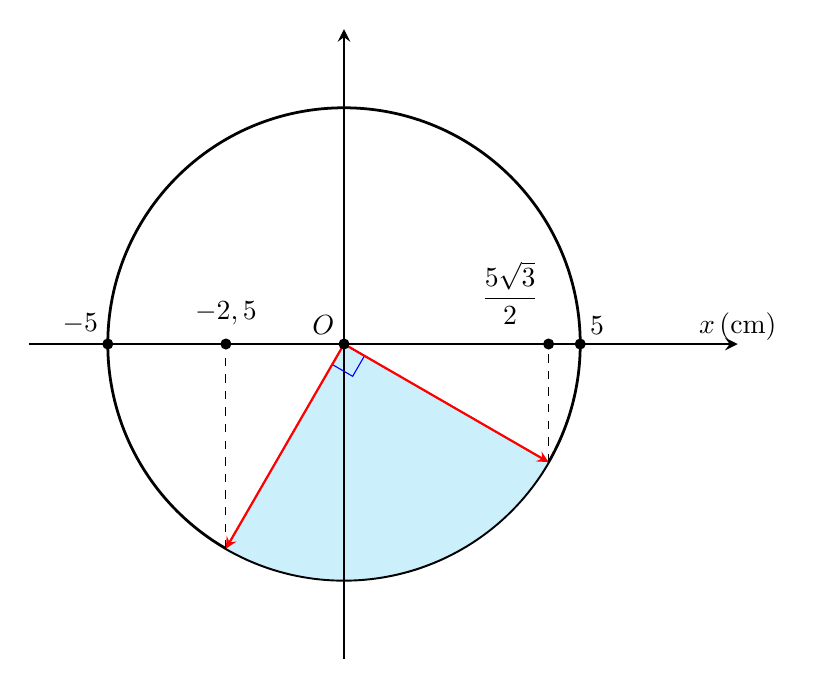
\begin{tikzpicture}
		\coordinate (O) at (0,0);
		\coordinate (A) at (240:3);
		\coordinate (B) at (330:3);
		\coordinate (D) at (5,0);
		\coordinate (E) at (-4,0);
		\draw[line width=1.0] (O) circle[radius=3];
		
		\draw [fill=cyan!20](330:3)--(0,0)--(240:3) arc (240:330:3)--cycle;
		\draw[-stealth, line width=1.0] (E) -- (D);
		\draw[-stealth, line width=1.0] (0,-4) -- (0,4);
		\tkzMarkRightAngle[size=0.3,color=blue](A,O,B);
		\draw[-stealth,thick,red] (O) -- (A);
		\draw[-stealth,thick,red] (O) -- (B);
		\draw[dashed] (A) -- ($(O)!(A)!(D)$);
		\draw[dashed] (B) -- ($(O)!(B)!(D)$);
		
		\fill   (O) circle[radius=2pt]  node [above left] {$O$};
		\fill   ($(O)!(A)!(D)$) circle[radius=2pt, color=teal];
		\fill   ($(O)!(B)!(E)$) circle[radius=2pt,color=teal];
		\fill   (3,0) circle[radius=2pt]  node [above right] {$5$};
		\fill   (-3,0) circle[radius=2pt]  node [above left] {$-5$};
		\node[label={[above]90:$x \left(\si{\centi\meter}\right)$}] at ($(D)-(0,0.2)$){};
		\node[label={[above]90:$-2,5$}] at ($(O)!(A)!(D)$){};
		\node[label={[above left]90:$\dfrac{5\sqrt{3}}{2}$}] at ($(O)!(B)!(D)$){};
	\end{tikzpicture}
\end{center}
Dựa vào vòng tròn lượng giác, thời gian ngắn nhất để vật đi từ vị trí $x_1=\SI{-2.5}{\centi\meter}$ đến vị trí $x_2=\xsi{\dfrac{5\sqrt{3}}{2}}{\centi\meter}$
 là
 $$\Delta t=\dfrac{T}{4}=\dfrac{1}{4}\cdot\dfrac{2\pi}{\omega}=\xsi{\dfrac{1}{8}}{\second}
.$$}

\item Một vật dao động điều hoà trên quỹ đạo dài $\SI{8}{\centi\meter}$. Tốc độ của vật khi qua vị trí cân bằng là $\xsi{0,4\pi}{\meter/\second}$. Gọi mốc thời gian là lúc vật đi qua vị trí $\xsi{2\sqrt{3}}{\centi\meter}$ theo chiều dương. Phương trình dao động của vật là
\begin{mcq}(2)
	\item $x=\xsi{4\cos\left(10\pi t-\dfrac{\pi}{6}\right)}{\centi\meter}$.
	\item $x=\xsi{4\cos\left(10\pi t+\dfrac{\pi}{6}\right)}{\centi\meter}$.
	\item $x=\xsi{2\cos\left(10\pi t-\dfrac{\pi}{6}\right)}{\centi\meter}$.
	\item $x=\xsi{2\cos\left(10\pi t+\dfrac{\pi}{6}\right)}{\centi\meter}$.
\end{mcq}
\hideall{
\textbf{Đáp án A.}\\
Biên độ dao động của vật
$$A=\dfrac{L}{2}=\SI{4}{\centi\meter}$$
Tần số góc dao động
$$\omega=\dfrac{v_\text{max}}{A}=\dfrac{\xsi{40\pi}{\radian/\second}}{\SI{4}{\centi\meter}}=\xsi{10\pi}{\radian/\second}$$
Chọn mốc thời gian lúc vật đi qua vị trí $\xsi{2\sqrt{3}}{\centi\meter}$ theo chiều dương. Pha ban đầu
$$\varphi_0=-\arccos\dfrac{x_0}{A}=-\xsi{\dfrac{\pi}{6}}{\radian}$$
}

\item Một vật dao động điều hoà trên trục $Ox$. Khi vật qua vị trí cân bằng thì tốc độ của nó là $\SI{20}{\centi\meter/\second}$. Khi vật có tốc độ là $\SI{10}{\centi\meter/\second}$ thì gia tốc của nó có độ lớn $\xsi{40\sqrt{3}}{\centi\meter/\second^2}$. Biên độ dao động của vật bằng
\begin{mcq}(4)
	\item $\SI{4}{\centi\meter}$.
	\item $\SI{5}{\centi\meter}$.
	\item $\SI{16}{\centi\meter}$.
	\item $\SI{8}{\centi\meter}$.
\end{mcq}
\hideall{
\textbf{Đáp án B.}\\
$$\dfrac{v^2}{v^2_\text{max}}+\dfrac{a^2}{a^2_\text{max}}=1\Rightarrow a_\text{max}=\SI{80}{\centi\meter/\second^2}$$
Biên độ dao động của vật:
$$A=\dfrac{v^2_\text{max}}{a_\text{max}}=\SI{5}{\centi\meter}.$$
}

\item Đồ thị động năng theo thời gian của một vật có khối lượng $\SI{0.4}{\kilogram}$ dao động điều hoà. Tại thời điểm ban đầu vật đang chuyển động theo chiều dương. Lấy $\pi^2=10$. Phương trình dao động của vật có dạng
\begin{center}
	\begin{tikzpicture}  
		\begin{axis}[  ultra thick,
			xmin=0,  
			xmax=1.2,  
			xtick={0,1.0},
			ytick={0,2},
			minor x tick num=5,
			minor y tick num=3,
			yticklabels=\empty,
			xticklabels=\empty,
			ymin=0,  
			ymax=2.5, 
			y=1.5cm,
			samples=300,
			axis lines=center, 
			grid style={step=1, color=gray!60!white},
			grid=both,
			xlabel=$t\ \left(\si{\second}\right)$, 
			ylabel=$W_\text{đ}\ \left(\si{\joule}\right)$, 
			every axis y label/.style={at=(current axis.above origin),anchor=south},  
			every axis x label/.style={at=(current axis.right of origin),anchor=west},  ]
			\addplot [ultra thick, blue, smooth, domain=0:1.0] {1+1*cos(deg(4*pi*x+pi/3))}; 
		\end{axis}  
		\node[label={[left]90:0}] at (0,0){};
		\node[label={[left]90:0,02}] at (0,2.9){};
		\node[label={[below]90:$\dfrac{1}{6}$}] at (1,-0.1){};
	\end{tikzpicture}
\end{center}
\begin{mcq}(2)
	\item $x=\xsi{5\cos\left(2\pi t+\dfrac{\pi}{3}\right)}{\centi\meter}$.
	\item $x=\xsi{10\cos\left(2\pi t+\dfrac{5\pi}{6}\right)}{\centi\meter}$.
	\item $x=\xsi{10\cos\left(2\pi t-\dfrac{5\pi}{6}\right)}{\centi\meter}$.
	\item $x=\xsi{5\cos\left(2\pi t-\dfrac{\pi}{3}\right)}{\centi\meter}$.
\end{mcq}
\hideall{
\textbf{Đáp án D.}\\
Chu kì dao động của động năng:
$$2T'=6\cdot\left(\xsi{\dfrac{1}{6}}{\second}\right)=\SI{1}{\second}\Rightarrow T'=\SI{0.5}{\second}$$
Chu kì dao động của vật:
$$T=2T'=\SI{1}{\second}$$
Ban đầu vật ở vị trí có $\dfrac{W_\text{đ}}{W}=\dfrac{\SI{0.015}{\joule}}{\SI{0.02}{\joule}}=\dfrac{3}{4}\Rightarrow W_\text{t}=\dfrac{W}{4}\Leftrightarrow x=\pm\dfrac{A}{2}$ và tốc độ đang giảm (đang chuyển động về vị trí biên).\\
Kết hợp với dữ kiện đề bài, ban đầu vật chuyển động theo chiều dương nên vị trí ban đầu của vật ứng với $x=\dfrac{A}{2}$.\\
Pha ban đầu của dao động:
$$\varphi_0=-\arccos\dfrac{x_0}{A}=\arccos\dfrac{1}{2}=-\xsi{\dfrac{\pi}{3}}{\radian}$$
Phương trình dao động của vật:
$$x=\xsi{5\cos\left(2\pi t-\dfrac{\pi}{3}\right)}{\centi\meter}.$$
}
\end{enumerate}
\section{Tự luận \textit{(4,0 điểm)}}
\begin{enumerate}[label=\bfseries Bài \arabic*:]
	\item Cho đồ thị vận tốc theo thời gian của một vật dao động điều hòa như hình vẽ. Biết rằng khối lượng của vật là $\SI{150}{\gram}$. Hãy xác định
	\begin{center}
		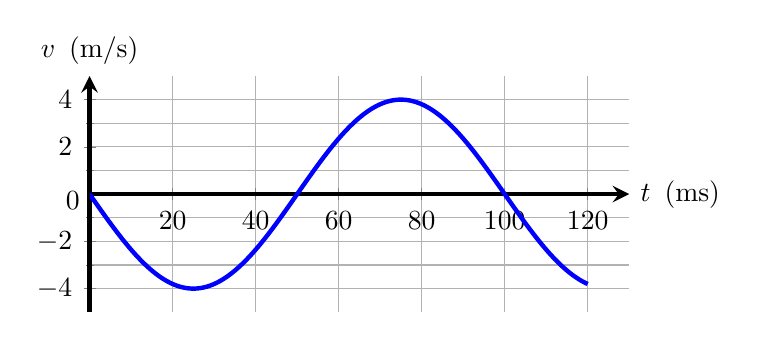
\begin{tikzpicture}  
			\begin{axis}[  ultra thick,
				xmin=0,  
				xmax=130,  
				xtick={0,20,40,60,...,120},
				ytick={-4,-2,0,2,4},
				minor x tick num=0,
				minor y tick num=1,
				ymin=-5,  
				ymax=5, 
				y=0.3cm,
				samples=300,
				axis lines=center, 
				grid style={step=1, color=gray!60!white},
				grid=both,
				xlabel=$t\ \left(\si{\milli\second}\right)$, 
				ylabel=$v\ \left(\si{\meter/\second}\right)$, 
				every axis y label/.style={at=(current axis.above origin),anchor=south},  
				every axis x label/.style={at=(current axis.right of origin),anchor=west},  ]
				\addplot [ultra thick, blue, smooth, domain=0:120] {4*cos(deg(0.02*pi*x+pi/2))}; 
			\end{axis}  
			\node[label={[left]90:0}] at (0,1.3){};
		\end{tikzpicture}
	\end{center}
	\begin{enumerate}[label=\alph*)]
		\item chu kì dao động của vật.
		\item biên độ dao động của vật.
		\item cơ năng của vật dao động.
		\item vị trí và gia tốc của vật tại thời điểm $\SI{100}{\milli\second}$.
	\end{enumerate}
\hideall{
\begin{enumerate}[label=\alph*)]
	\item Chu kì dao động của vật:
	$$T=\SI{100}{\milli\second}$$
	\item Tần số góc dao động:
	$$\omega=\dfrac{2\pi}{T}=\xsi{20\pi}{\radian/\second}$$
	Biên độ dao động của vật:
	$$A=\dfrac{v_\text{max}}{\omega}=\dfrac{\SI{4E2}{\centi\meter/\second}}{\xsi{20\pi}{\radian/\second}}\approx\SI{6.37}{\centi\meter}$$
	\item Cơ năng của vật dao động:
	$$W=W_\text{đ max}=\dfrac{1}{2}mv^2_\text{max}=\dfrac{1}{2}\cdot\left(\SI{0.15}{\kilogram}\right)\cdot\left(\SI{4}{\meter/\second}\right)^2=\SI{1.2}{\joule}$$
	\item Tại thời điểm $t=\SI{100}{\milli\second}$ vật có vận tốc bằng 0 và đang giảm $\Rightarrow$ vật ở vị trí biên dương $x=A=\SI{6.37}{\centi\meter}$.\\
	Gia tốc của vật lúc này:
	$$a=-\omega^2 x=-\left(\xsi{20\pi}{\radian/\second}\right)^2\cdot\left(\SI{6.37}{\centi\meter}\right)\approx\SI{25147.75}{\centi\meter/\second^2}.$$
\end{enumerate}

}
\item Quả lắc của đồng hồ cổ treo tường có tác dụng vận hành cho đồng hồ chạy đúng giờ.\\
\begin{minipage}[l]{0.55\textwidth}
	Cứ sau mỗi chu kì dao động của quả lắc, do sức cản và việc vận hành hệ thống bánh răng để các kim đồng hồ chạy nên nó tiêu hao năng lượng $\Delta E=\SI{0.100}{\milli\joule}$. Năng lượng này được lấy từ một quả tạ có trọng lượng $P=\SI{50.0}{\newton}$ treo trong hoặc ngoài đồng hồ.
	\begin{enumerate}[label=\alph*)]
		\item Vì sao sau một thời gian dài đồng hồ chạy thì quả tạ bị hạ thấp xuống và ta lại phải đưa nó lên cao?
		\item Nếu chạy trong thời gian $t=10\ \text{ngày}$ thì quả tạ sẽ giảm độ cao bao nhiêu mét? Biết trong 30 chu kì dao động của quả lắc thì kim giây chuyển động được một vòng.
	\end{enumerate}
\end{minipage}
\begin{minipage}[c]{0.05\textwidth}
	\
\end{minipage}
\begin{minipage}[l]{0.4\textwidth}
	\begin{center}
		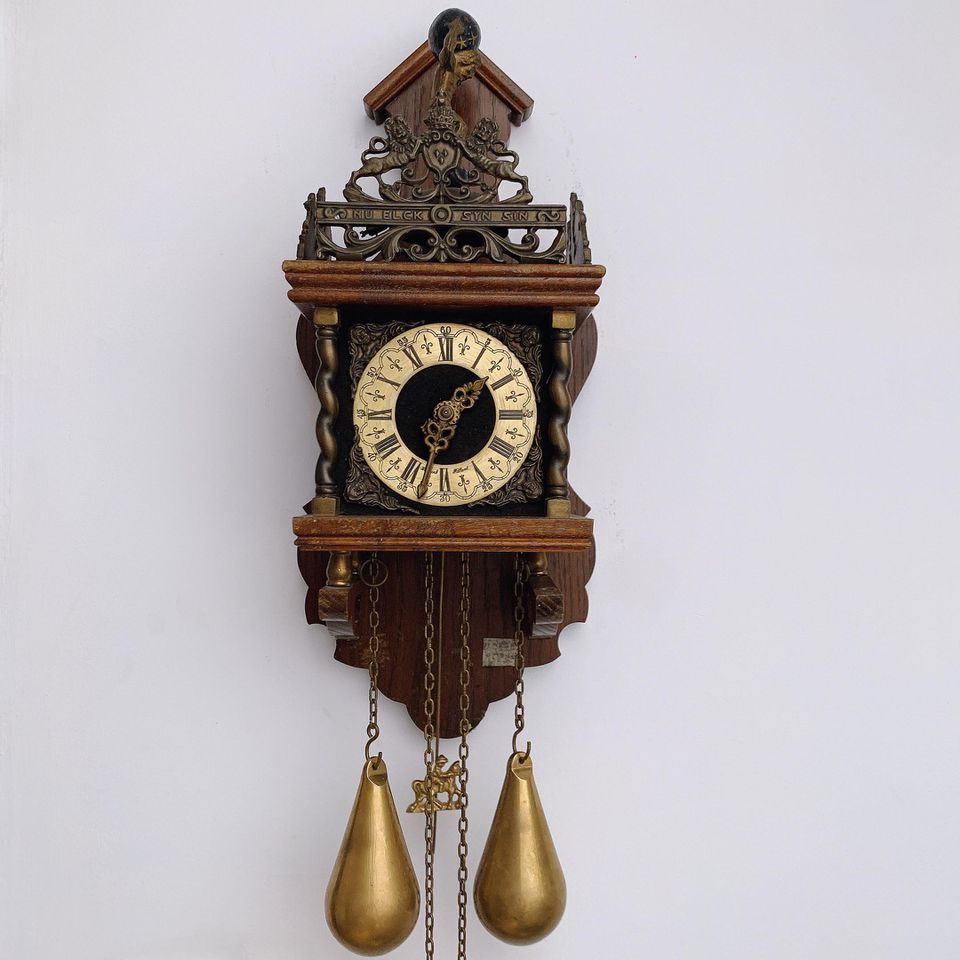
\includegraphics[width=0.5\linewidth]{../figs/D11-2-2}
		\captionof{figure}{Hai quả tạ là nguồn năng lượng cung cấp để dao động của quả lắc không bị tắt (một quả dùng cho hệ thống chuông).}
	\end{center}
\end{minipage}
\hideall{
\begin{enumerate}[label=\alph*)]
	\item Quả tạ dự trữ năng lượng dưới dạng thế năng trọng trường. Mỗi chu kì dao động, thế năng này giảm dần đề bù cho phần năng lượng tiêu hao của quả lắc và hệ thống bánh răng. Do đó, độ cao quả tạ giảm dần.
	\item Mỗi phút, kim giây chuyển động hết 1 vòng và con lắc đồng hồ thực hiện 30 chu kì.\\
	Như vậy, số chu kì con lắc thực hiện được trong 10 ngày là:
	$$N=10 \cdot24\cdot\left(\SI{60}{\minute}\right)\cdot\left(30\ \text{chu kì/\si{\minute}}\right)=432000\ \text{chu kì}$$
	Tổng năng lượng tiêu hao trong 10 ngày:
	$$E=\left(432000\ \text{chu kì}\right)\cdot\left(\SI{0.100E-3}{\joule/\text{chu kì}}\right)=\SI{43.2}{\joule}$$
	Năng lượng tiêu hao này được bù bằng độ giảm thế năng trọng trường của quả tạ. Do đó, độ cao quả tạ bị giảm một đoạn:
	$$\Delta h=\dfrac{E}{P}=\dfrac{\SI{43.2}{\joule}}{\SI{50.0}{\newton}}=\SI{0.864}{\meter}.$$
	
\end{enumerate}

}
\end{enumerate}
%\chapter{Đề 3}
%\begin{center}
	ĐỀ ÔN TẬP KIỂM TRA GIỮA HỌC KỲ I – MÔN VẬT LÝ 11\\
	Thời gian làm bài: 50 phút \\
	(Không kể thời gian phát đề)\\
\end{center}
\ANSMCQ{
	\begin{center}
		\begin{tabular}{|m{2.8em}|m{2.8em}|m{2.8em}|m{2.8em}|m{2.8em}|m{2.8em}|m{2.8em}|m{2.8em}|m{2.8em}|m{2.8em}|}
			\hline
			1D & 2D & 3B & 4A & 5D & 6C & 7C & 8A & 9D & 10A\\
			\hline
			11D & 12A & 13D & 14C & 15D & 16B & 17C & 18B & 19B & 20B\\
			\hline
			21C & 22C & 23C & 24D & 25B & 26C & 27C & 28B & 29D & 30C\\
			\hline
		\end{tabular}
\end{center}}
\begin{enumerate}[label=\bfseries Câu \arabic*:]
	\item Một chất điểm dao động điều hòa trên trục $Ox$. Vectơ gia tốc của chất điểm có
	\begin{mcq}
		\item độ lớn cực đại ở vị trí biên, chiều luôn hướng ra biên.
		\item độ lớn cực tiểu khi qua vị trí cân bằng luôn cùng chiều với vectơ vận tốc.
		\item độ lớn không đổi, chiều luôn hướng về vị trí cân bằng.
		\item độ lớn tỉ lệ với độ lớn của li độ, chiều luôn hướng về vị trí cân bằng.
	\end{mcq}
\hideall{
\textbf{Đáp án D.}
}

\item Phát biểu nào sau đây là \textbf{sai}? Cơ năng của dao động điều hòa bằng 
\begin{mcq}
	\item động năng của vật khi đi qua vị trí cân bằng.
	\item tổng động năng và thế năng ở thời điểm bất kì.
	\item thế năng của vật ở vị trí biên.
	\item động năng ở thời điểm ban đầu.
\end{mcq}
\hideall{
\textbf{Đáp án D.}\\
Động năng ở thời điểm ban đầu không phải lúc nào cũng là động năng cực đại.
}

\item Chu kì dao động điều hòa là
\begin{mcq}
	\item khoảng thời gian để vật đi từ biên này sang biên kia.
	\item khoảng thời gian ngắn nhất để vật lặp lại trạng thái dao động.
	\item số dao động toàn phần vật thực hiện được trong $\SI{1}{\second}$.
	\item khoảng thời gian ngắn nhất để vật trở lại vị trí ban đầu.
\end{mcq}
\hideall{
\textbf{Đáp án B.}
}

\item Phát biểu nào sau đây là \textbf{sai} khi nói về dao động tắt dần?
\begin{mcq}
	\item Tần số của dao động càng lớn thì dao động tắt dần càng nhanh.
	\item Cơ năng của dao động giảm dần.
	\item Biên độ của dao động giảm dần.
	\item Lực cản càng lớn thì sự tắt dần càng nhanh.
\end{mcq}
\hideall{
\textbf{Đáp án A.}\\
Tần số của dao động càng lớn thì năng lượng dao động càng lớn, do đó sự tắt dần diễn ra càng chậm.
}

\item Con lắc đơn gồm vật nhỏ khối lượng $m$ được nối với dây treo nhẹ, không dãn. Kích thích cho con lắc dao động điều hoà thì tần số dao động của con lắc là $f$. Nếu giảm khối lượng vật nhỏ đi 2 lần thì tần số dao động của con lắc sẽ
\begin{mcq}(4)
	\item tăng $\sqrt{2}$ lần.
	\item giảm $\sqrt{2}$ lần
	\item giảm 2 lần.
	\item không đổi.
\end{mcq}
\hideall{
\textbf{Đáp án D.}\\
Tần số dao động của con lắc đơn không phụ thuộc vào khối lượng vật nặng
$$f=\dfrac{1}{2\pi}\sqrt{\dfrac{g}{\ell}}.$$
}

\item Vật nhỏ dao động điều hoà với biên độ $A$, tốc độ của vật lớn nhất khi
\begin{mcq}(2)
	\item vật ở vị trí biên âm.	
	\item vật ở vị trí biên dương.
	\item vật ở vị trí cân bằng.	
	\item vật ở vị trí có li độ $A/3$.
\end{mcq}
\hideall{
\textbf{Đáp án C.}
}

\item Dao động duy trì là dao động tắt dần mà người ta đã
\begin{mcq}
	\item Làm mất lực cản của môi trường đối với vật chuyển động.
	\item Tác dụng vào vật một ngoại lực biến đổi điều hòa theo thời gian.
	\item Cung cấp cho vật một phần năng lượng đúng bằng năng lượng của vật bị tiêu hao trong từng chu kì.
	\item Kích thích lại dao động sau khi dao động bị tắt hẳn.
\end{mcq}
\hideall{
\textbf{Đáp án C.}
}

\item Thế năng của con lắc đơn tại vị trí có li độ dài $s$ được xác định bởi công thức
\begin{mcq}(4)
	\item $W_\text{t}=\dfrac{1}{2}mg\dfrac{s^2}{\ell}$.
	\item $W_\text{t}=\dfrac{1}{2}mg\ell s^2$.
	\item $W_\text{t}=\dfrac{1}{2}mg\dfrac{s^2}{\ell^2}$.
	\item $W_\text{t}=\dfrac{1}{2}mg\dfrac{s}{\ell}$.
\end{mcq}
\hideall{
\textbf{Đáp án A.}
}

\item Một con lắc lò xo gồm vật nhỏ và lò xo nhẹ, dao động điều hòa trên mặt phẳng nằm ngang không ma sát. Động năng của con lắc đạt giá trị cực đại khi
\begin{mcq}(2)
	\item lò xo có chiều dài cực đại.
	\item vật có tốc độ cực tiểu.
	\item vật đi qua vị trí biên âm.
	\item lò xo không biến dạng.
\end{mcq}
\hideall{
\textbf{Đáp án D.}\\
Đối với con lắc lò xo dao động trên mặt phẳng nằm ngang không ma sát thì vị trí lò xo không biến dạng trùng với vị trí cân bằng của vật nặng. Khi vật qua VTCB thì vật đạt tốc độ cực đại, do đó động năng của vật đạt cực đại.
}

\item Khi nói về năng lượng của một vật dao động điều hòa, phát biểu nào sau đây là \textbf{đúng}?
\begin{mcq}
	\item Cứ mỗi chu kì dao động của vật, có bốn thời điểm thế năng bằng động năng.
	\item Thế năng của vật đạt cực đại khi vật ở vị trí cân bằng.
	\item Động năng của vật đạt cực đại khi vật ở vị trí biên.
	\item Thế năng và động năng của vật biến thiên cùng tần số với tần số của li độ.
\end{mcq}
\hideall{
\textbf{Đáp án A.}\\
Cứ mỗi chu kì dao động của vật, có bốn thời điểm thế năng bằng động năng ứng với vị trí $x=\pm\dfrac{A}{\sqrt{2}}$.\\
Thế năng của vật đạt cực đại khi vật ở vị trí biên.\\
Động năng của vật đạt cực đại khi vật ở vị trí cân bằng.\\
Thế năng và động năng của vật biến thiên với tần số gấp 2 lần tần số của li độ.
}

\item Một vật dao động điều hòa trên trục $Ox$. Hình bên là đồ thị biểu diễn sự phụ thuộc của li độ $x$ vào thời gian $t$. Tần số của dao động là 
\begin{center}
	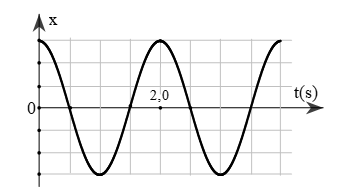
\includegraphics[width=0.4\linewidth]{../figs/D11-3-3}
\end{center}
\begin{mcq}(4)
	\item $\SI{2.0}{\hertz}$.
	\item $\SI{1.0}{\hertz}$.
	\item $\SI{1.5}{\hertz}$.
	\item $\SI{0.5}{\hertz}$.
\end{mcq}
\hideall{
\textbf{Đáp án D.}\\
Chu kì dao động của vật $T=\SI{2.0}{\second}$.\\
Tần số dao động của vật:
$$f=\dfrac{1}{T}=\SI{0.5}{\hertz}.$$
}

\item Trên hình vẽ là một hệ dao động. Khi cho con lắc M dao động, thì các con lắc (1), (2), (3), (4) cũng dao động cưỡng bức theo. Hỏi con lắc nào dao động mạnh nhất trong 4 con lắc?
\begin{center}
	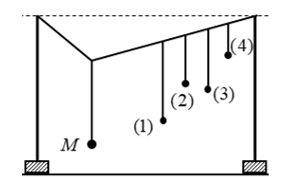
\includegraphics[width=0.4\linewidth]{../figs/D11-3-8}
\end{center}
\begin{mcq}(4)
	\item (1).
	\item (2).
	\item (3).
	\item (4)
\end{mcq}
\hideall{
\textbf{Đáp án A.}\\
Khi con lắc M dao động sẽ làm cho các con lắc còn lại dao động cường bức theo. Vì chiều dài con lắc (1) gần bằng chiều dài con lắc M nên chu kì dao động riêng của (1) xấp xỉ chu kì dao động riêng của M $\Rightarrow$ (1) dao động mạnh nhất.
}

\item Đồ thị biểu diễn li độ theo thời gian của một vật được mô tả như hình. Tốc độ của vật khi qua vị trí cân bằng là
\begin{center}
	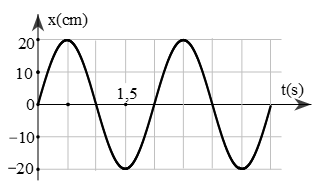
\includegraphics[width=0.4\linewidth]{../figs/D11-3-1}
\end{center}
\begin{mcq}(4)
	\item $\SI{62.8}{\meter/\second}$.
	\item $\SI{30.0}{\centi\meter/\second}$.
	\item $\SI{41.9}{\centi\meter/\second}$.
	\item $\SI{62.8}{\centi\meter/\second}$.
\end{mcq}
\hideall{
\textbf{Đáp án D.}\\
Tần số góc dao động:
$$T=\SI{2}{\second}\Rightarrow\omega=\dfrac{2\pi}{T}=\xsi{\pi}{\radian/\second}$$
Tốc độ của vật khi qua VTCB:
$$v_\text{max}=\omega A=\left(\xsi{\pi}{\radian/\second}\right)\cdot\left(\SI{20}{\centi\meter}\right)\approx\SI{62.8}{\centi\meter/\second}.$$
}

\item Một vật dao động điều hoà trên trục $Ox$. Hình bên là đồ thị biểu diễn sự phụ thuộc của li độ $x$ vào thời gian $t$. Pha ban đầu của dao động là
\begin{center}
	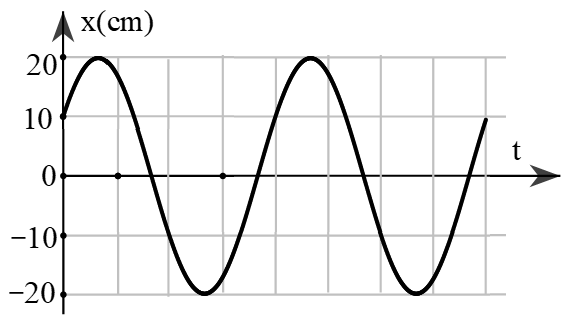
\includegraphics[width=0.4\linewidth]{../figs/D11-3-4}
\end{center}
\begin{mcq}(4)
	\item $\xsi{\dfrac{\pi}{6}}{\radian}$.
	\item $\xsi{\dfrac{\pi}{3}}{\radian}$.
	\item $-\xsi{\dfrac{\pi}{3}}{\radian}$.
	\item $-\xsi{\dfrac{\pi}{6}}{\radian}$.
\end{mcq}
\hideall{
\textbf{Đáp án C.}\\
Tại thời điểm ban đầu vật có li độ $x_0=\SI{10}{\centi\meter}$ và đang chuyển động theo chiều dương nên
$$\varphi_0=-\arccos\dfrac{x_0}{A}=-\xsi{\dfrac{\pi}{3}}{\radian}.$$
}

\item Một chất điểm dao động điều hoà có phương trình li độ $x=\xsi{6\cos\left(4\pi t-\dfrac{\pi}{3}\right)}{\centi\meter}$, thời gian $t$ tính bằng giây. Khoảng thời gian để chất điểm thực hiện được 5 dao động toàn phần là
\begin{mcq}(4)
	\item $\SI{30}{\second}$.
	\item $\SI{10}{\second}$.
	\item $\SI{2}{\second}$.
	\item $\SI{2.5}{\second}.$
\end{mcq}
\hideall{
\textbf{Đáp án D.}\\
Chu kì dao động của vật
$$T=\dfrac{2\pi}{\omega}=\SI{0.5}{\second}$$
Thời gian chất điểm thực hiện được 5 dao động là:
$$\Delta t=5T=\SI{2.5}{\second}.$$
}

\item Một vật dao động điều hoà có phương trình li độ $x=\xsi{5\cos\left(2\pi t-\dfrac{\pi}{6}\right)}{\centi\meter}$. Lấy $\pi^2=10$. Khi vật có li độ $x=\SI{3}{\centi\meter}$ gia tốc của vật là
\begin{mcq}(4)
	\item $\SI{12}{\meter/\second^2}$.
	\item $\SI{-120}{\centi\meter/\second^2}$.
	\item $\SI{1.20}{\centi\meter/\second^2}$.
	\item $\SI{12}{\centi\meter/\second^2}$.
\end{mcq}
\hideall{
\textbf{Đáp án B.}\\
Gia tốc của vật tại vị trí có li độ $x=\SI{3}{\centi\meter}$:
$$a=-\omega^2x=-\left(\xsi{2\pi}{\radian/\second}\right)^2\cdot\left(\SI{3}{\centi\meter}\right)\approx-\SI{120}{\centi\meter/\second^2}.$$
}

\item Một con lắc lò xo gồm vật năng khối lượng $\SI{400}{\gram}$ được nối với lò xo có độ cứng $\SI{100}{\newton/\meter}$. Kéo vật nặng ra khỏi vị trí cân bằng $\SI{2}{\centi\meter}$ rồi truyền cho nó tốc độ đầu $\xsi{15\sqrt{5}\pi}{\centi\meter/\second}$. Lấy $\pi^2=10$. Năng lượng dao động của vật là
\begin{mcq}(4)
	\item $\SI{245}{\joule}$.
	\item $\SI{2.45}{\joule}$.
	\item $\SI{0.245}{\joule}$.
	\item $\SI{24.5}{\joule}$.
\end{mcq}
\hideall{
\textbf{Đáp án C.}\\
Năng lượng dao động của vật là
$$W=W_\text{t}+W_\text{đ}=\dfrac{1}{2}kx^2+\dfrac{1}{2}mv^2=\SI{0.245}{\joule}.$$
}

\item Một vật dao động điều hoà với phương trình li độ $x=A\cos\left(2\pi ft+\varphi_0\right)$. Khi vật ở vị trí cân bằng thì vận tốc của vật có độ lớn
\begin{mcq}(4)
	\item $4\pi^2f^2A$.
	\item $2\pi fA$.
	\item $\pi^2f^2A$.
	\item $\pi f A$.
\end{mcq}
\hideall{
\textbf{Đáp án B.}
}
\item Một vật dao động điều hòa trong $\SI{20}{\second}$ vật thực hiện được 10 dao động toàn phần. Động năng của vật biến thiên với chu kì bằng
\begin{mcq}(4)
	\item $\SI{2.0}{\second}$.
	\item $\SI{1.0}{\second}$.
	\item $\SI{4.0}{\second}$.
	\item $\SI{0.5}{\second}$.
\end{mcq}
\hideall{
\textbf{Đáp án B.}\\
Chu kì dao động của vật:
$$T=\dfrac{\Delta t}{N}=\SI{2.0}{\second}$$
Động năng biến thiên với chu kì:
$$T'=\dfrac{T}{2}=\SI{1.0}{\second}.$$
}

\item Một vật dao động điều hoà với biên độ $A$, chu kì $T$. Thời gian ngắn nhất để vật đi từ vị trí có li độ $\dfrac{A}{2}$ đến $-\dfrac{A\sqrt{3}}{2}$ là
\begin{mcq}(4)
	\item $\dfrac{T}{8}$.
	\item $\dfrac{T}{4}$.
	\item $\dfrac{T}{6}$.
	\item $\dfrac{T}{12}$.
\end{mcq}
\hideall{
\textbf{Đáp án B.}\\
Dùng vòng tròn lượng giác hoặc trục thời gian, thời gian ngắn nhất để vật đi từ li độ $\dfrac{A}{2}$ đến li độ $-\dfrac{A\sqrt{3}}{2}$ là $\dfrac{T}{4}$.
}

\item Một vật nhỏ đang dao động điều hoà với biên độ $\SI{4}{\centi\meter}$ trên trục $Ox$, gốc toạ độ được chọn trùng với vị trí cân bằng của vật. Tại thời điểm pha của dao động là $\xsi{\dfrac{2\pi}{3}}{\radian}$ thì vật có li độ
\begin{mcq}
	\item $\SI{2}{\centi\meter}$ và chuyển động theo chiều dương trục $Ox$.
	\item $\xsi{2\sqrt{2}}{\centi\meter}$ và chuyển động theo chiều âm trục $Ox$.
	\item $\SI{-2}{\centi\meter}$ và chuyển động theo chiều âm trục $Ox$.
	\item $\SI{-2}{\centi\meter}$ và chuyển động theo chiều dương trục $Ox$.
\end{mcq}
\hideall{
\textbf{Đáp án C.}\\
Li độ của vật tại thời điểm pha dao động $\varphi=\xsi{\dfrac{2\pi}{3}}{\radian}$
$$x=A\cos\varphi=-\SI{2}{\centi\meter}$$
Vận tốc của vật
$$v=-\omega A\sin\varphi>0$$
Do đó, vật có li độ $\SI{-2}{\centi\meter}$ và chuyển động theo chiều âm trục $Ox$.
}

\item Một vật dao động điều hoà có vận tốc và li độ tại thời điểm $t_1$ và $t_2$ tương ứng là $v_1=\SI{20}{\centi\meter/\second}$, $x_1=\xsi{8\sqrt{3}}{\centi\meter}$ và $v_2=\xsi{20\sqrt{2}}{\centi\meter/\second}$, $x_2=\xsi{8\sqrt{2}}{\centi\meter}$. Vận tốc của vật có độ lớn cực đại là
\begin{mcq}(4)
	\item $\xsi{40\sqrt{2}}{\centi\meter/\second}$.
	\item $\SI{80}{\centi\meter/\second}$.
	\item $\SI{40}{\centi\meter/\second}$.
	\item $\xsi{40\sqrt{3}}{\centi\meter/\second}$.
\end{mcq}
\hideall{
\textbf{Đáp án C.}\\
Áp dụng hệ thức độc lập thời gian:
$$x^2_1+\dfrac{v^2_1}{\omega^2}=x^2_2+\dfrac{v^2_2}{\omega^2}\Rightarrow \omega=\SI{2.5}{\radian/\second}$$
Biên độ dao động của vật:
$$A=\sqrt{x^2_1+\dfrac{v^2_1}{\omega^2}}=\SI{16}{\centi\meter}$$
Vận tốc cực đại của vật:
$$v_\text{max}=\omega A=\SI{40}{\centi\meter/\second}.$$
}

\item Một chất điểm dao động điều hoà với tần số góc $\omega=\pi\approx\xsi{\sqrt{10}}{\radian/\second}$. Biết rằng khi chất điểm có vận tốc $\xsi{3\pi}{\centi\meter/\second}$ thì gia tốc của nó là $\SI{40}{\centi\meter/\second^2}$. Biên độ dao động của chất điểm bằng
\begin{mcq}(4)
	\item $\SI{3}{\centi\meter}$.
	\item $\SI{4}{\centi\meter}$.
	\item $\SI{5}{\centi\meter}$.
	\item $\SI{6}{\centi\meter}$.
\end{mcq}
\hideall{
\textbf{Đáp án C.}\\
Biên độ dao động của chất điểm
$$A=\sqrt{\dfrac{v^2}{\omega^2}+\dfrac{a^2}{\omega^2}}=\SI{5}{\centi\meter}.$$
}

\item Hình bên là hai đường hình sin biểu diễn hai trong ba đại lượng: li độ $x$, vận tốc $v$ và gia tốc $a$ theo thời gian $t$. Đường số (1) và đường số (2) lần lượt biểu diễn cho
\begin{center}
	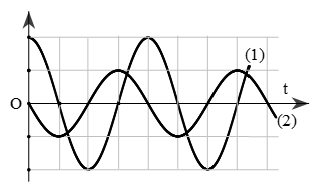
\includegraphics[width=0.4\linewidth]{../figs/D11-3-2}
\end{center}
\begin{mcq}(2)
	\item  gia tốc và vận tốc.
	\item gia tốc và li độ.
	\item vận tốc và li độ.
	\item li độ và vận tốc.
\end{mcq}
\hideall{
\textbf{Đáp án D.}\\
Nhận thấy đồ thị (2) sớm pha $\xsi{\dfrac{\pi}{2}}{\radian}$ so với đồ thị (1) nên (1) và (2) tương ứng chỉ có thể là li độ và vận tốc hoặc vận tốc và gia tốc.
}

\item Chất điểm dao động điều hoà với chu kì $\SI{2}{\second}$. Tại thời điểm $t_1$ chất điểm có li độ $\SI{3}{\centi\meter}$ và đang chuyển động theo chiều dương, sau đó tại thời điểm $t_2=t_1+\SI{0.5}{\second}$ chất điểm có li độ $\SI{4}{\centi\meter}$. Từ thời điểm $t_1$ đến thời điểm $t_2$ chất điểm có tốc độ trung bình là
\begin{mcq}(4)
	\item $\SI{2}{\centi\meter/\second}$.
	\item $\SI{6}{\centi\meter/\second}$.	
	\item $\SI{14}{\centi\meter/\second}$.
	\item $\SI{10}{\centi\meter/\second}$.
\end{mcq}
\hideall{
\textbf{Đáp án B.}\\
Li độ độ của chất điểm tại 2 thời điểm $t_1$ và $t_2$ lệch pha nhau $\xsi{\dfrac{\pi}{2}}{\radian}$ vì $\Delta t=t_2-t_2=\dfrac{T}{4}$.\\
Biên độ dao động của chất điểm:
$$A=\sqrt{x^2_1+x^2_2}=\SI{5}{\centi\meter}$$
Quãng đường chất điểm đi được từ thời điểm $t_1$ đến thời điểm $t_2$:
$$s=A-x_1+A-x_2=\SI{3}{\centi\meter}$$
Tốc độ trung bình của chất điểm trong khoảng thời gian trên:
$$v_\text{tb}=\dfrac{s}{\Delta t}=\dfrac{\SI{3}{\centi\meter}}{\SI{0.5}{\second}}=\SI{6}{\centi\meter/\second}.$$

}

\item Hình bên là đồ thị biểu diễn sự phụ thuộc li độ $x$ theo thời gian $t$ của một vật dao động điều hòa. Phương trình dao động của vật là 
\begin{center}
	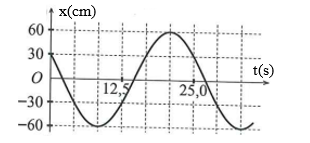
\includegraphics[width=0.4\linewidth]{../figs/D11-3-5}
\end{center}
\begin{mcq}(2)
	\item $x=\xsi{60\cos\left(\dfrac{4\pi}{45}t-\dfrac{\pi}{6}\right)}{\centi\meter}$.
	\item $x=\xsi{60\cos\left(\dfrac{4\pi}{45}t-\dfrac{\pi}{3}\right)}{\centi\meter}$.
	\item $x=\xsi{60\cos\left(\dfrac{2\pi}{25}t+\dfrac{\pi}{3}\right)}{\centi\meter}$.
	\item $x=\xsi{60\cos\left(\dfrac{4\pi}{45}t+\dfrac{\pi}{6}\right)}{\centi\meter}$.
\end{mcq}
\hideall{
\textbf{Đáp án C.}\\
Chu kì dao động của vật:
$$T=\SI{25}{\second}$$
Tần số góc dao động:
$$\omega=\dfrac{2\pi}{T}=\xsi{\dfrac{2\pi}{25}}{\radian/\second}$$
Tại thời điểm ban đầu, vật qua vị trí $x_0=\SI{30}{\centi\meter}$ theo chiều âm nên pha ban đầu
$$\varphi_0=\arccos\dfrac{x_0}{A}=\xsi{\dfrac{\pi}{3}}{\radian}$$
Phương trình dao động của vật:
$$x=\xsi{60\cos\left(\dfrac{2\pi}{25}t+\dfrac{\pi}{3}\right)}{\centi\meter}.$$
}

\item Con lắc đơn gồm vật nặng khối lượng $\SI{500}{\gram}$ được nối với sợi dây nhẹ, không dãn, đầu trên của dây được nối vào điểm cố định. Kích thích cho con lắc dao động tại nơi có gia tốc trọng trường $g=\SI{10}{\meter/\second^2}$. Lực căng của dây treo khi con lắc ở vị trí góc lệch cực đại so với phương thẳng đứng là $\SI{4}{\newton}$. Khi vật qua vị trí cân bằng thì lực căng của dây treo có độ lớn
\begin{mcq}(4)
	\item $\SI{11}{\newton}$.
	\item $\SI{5}{\newton}$.
	\item $\SI{7}{\newton}$.
	\item $\SI{3}{\newton}$.
\end{mcq}
\hideall{
\textbf{Đáp án C.}\\
Lực căng dây treo khi vật ở vị trí có góc lệch $\alpha$ so với phương thẳng đứng
$$T=mg\left(3\cos\alpha-2\cos\alpha_0\right)$$
Khi vật ở vị trí biên $\alpha=\alpha_0$
$$T_\text{biên}=mg\cos\alpha_0=\SI{4}{\newton}$$
Khi vật qua vị trí cân bằng $\alpha=\SI{0}{\radian}$:
$$T_\text{CB}=mg\left(3-2\cos\alpha_0\right)=3mg-2mg\cos\alpha_0=3\cdot\left(\SI{0.5}{\kilogram}\right)\cdot\left(\SI{10}{\meter/\second^2}\right)-2\cdot\left(\SI{4}{\newton}\right)=\SI{7}{\newton}.$$

}

\item Con lắc lò xo gồm vật nhỏ khối lượng $\SI{200}{\gram}$ nối vào đầu lò xo nhẹ, đầu còn lại của lò xo cố định vào tường. Người ta kích thích cho con lắc dao động điều hoà trên mặt phẳng nằm ngang, nhẵn. Khi vật nhỏ qua vị trí cân bằng thì nó có tốc độ $\SI{1}{\meter/\second}$. Khi vật nhỏ qua vị trí cách vị trí cân bằng đoạn $\xsi{2,5\sqrt{3}}{\centi\meter}$ thì nó có tốc độ $\SI{0.5}{\meter/\second}$. Lực đàn hồi do lò xo tác dụng lên vật nhỏ có giá trị lớn nhất là
\begin{mcq}(4)
	\item $\SI{2}{\newton}$.
	\item $\SI{4}{\newton}$.
	\item $\xsi{2\sqrt{3}}{\newton}$.
	\item $\xsi{4\sqrt{3}}{\newton}$.
\end{mcq}
\hideall{
\textbf{Đáp án B.}\\
Áp dụng hệ thức độc lập thời gian, suy ra được biên độ dao động của vật:
$$A=\dfrac{\left|x\right|}{\sqrt{1-\dfrac{v^2}{v^2_\text{max}}}}=\dfrac{\xsi{2,5\sqrt{3}}{\centi\meter}}{\sqrt{1-\left(\dfrac{\SI{0.5}{\meter/\second}}{\SI{1}{\meter/\second}}\right)^2}}=\SI{5}{\centi\meter}$$
Độ cứng của lò xo:
$$v_\text{max}=\omega A=A\sqrt{\dfrac{k}{m}}\Rightarrow k=\dfrac{v^2_\text{max}m}{A^2}=\SI{80}{\newton/\meter}$$
Lực đàn hồi cực đại của lò xo tác dụng lên vật nặng:
$$F_\text{đh max}=kA=\left(\SI{80}{\newton/\meter}\right)\cdot\left(\SI{0.05}{\meter}\right)=\SI{4}{\newton}.$$
}

\item Hai chất điểm A và B dao động điều hòa cùng tần số. Hình bên là đồ thị biểu diễn sự phụ thuộc li độ $x_1$ của chất điểm A và li độ $x_2$ của chất điểm B theo thời gian $t$. Hai chất điểm A và B lệch pha nhau
\begin{center}
	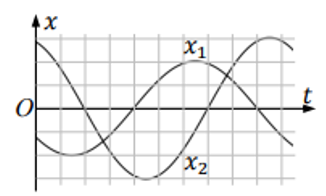
\includegraphics[width=0.35\linewidth]{../figs/D11-3-6}
\end{center}
\begin{mcq}(4)
	\item $\xsi{\dfrac{\pi}{6}}{\radian}$.
	\item $\xsi{\dfrac{\pi}{3}}{\radian}$.
	\item $\xsi{\dfrac{\pi}{12}}{\radian}$.
	\item $\xsi{\dfrac{3\pi}{5}}{\radian}$.
\end{mcq}
\hideall{
\textbf{Đáp án D.}\\
Hai vật dao động với cùng chu kì 
$$T=10\ \text{đv}$$
Sau khoảng thời gian $\Delta t=3\ \text{đv}$ thì vật 2 có cùng trạng thái dao động với vật 1 nên
$$\Delta \varphi=2\pi\cdot\dfrac{\Delta t}{T}=\xsi{\dfrac{3\pi}{5}}{\radian}.$$
}

\item Hai chất điểm A và B dao động điều hòa cùng phương, cùng tần số. Trong quá trình dao động, gia tốc của chất điểm A là $a_1$ và vận tốc của chất điểm B là $v_2$. Hình bên là đồ thị biễu diễn sự phụ thuộc của $a_1$ và $v_2$ theo thời gian $t$. Hai dao động điều hòa A và B lệch pha nhau
\begin{center}
	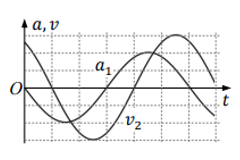
\includegraphics[width=0.35\linewidth]{../figs/D11-3-7}
\end{center}
\begin{mcq}(4)
	\item $\xsi{\dfrac{\pi}{3}}{\radian}$.
	\item $\xsi{\dfrac{5\pi}{6}}{\radian}$.
	\item $\xsi{\dfrac{\pi}{6}}{\radian}$.
	\item $\xsi{\dfrac{2\pi}{3}}{\radian}$.
\end{mcq}
\hideall{
\textbf{Đáp án C.}\\
Nhận thấy $a_1$ và $v_2$ có cùng chu kì dao động
$$T=\SI{6}{\text{đv}}$$
Sau khoảng thời gian $\Delta t=\SI{1}{\text{đv}}$ thì $v_2$ cùng pha $a_1$. Độ lệch pha $a_1$ và $v_2$:
$$\varphi_{a_1}-\varphi_{v_2}=2\pi\cdot\dfrac{\Delta t}{T}=\xsi{\dfrac{\pi}{3}}{\radian}.$$
Như vậy:
$$\varphi_{x_1}+\pi-\left(\varphi_{x_2}+\dfrac{\pi}{2}\right)=\dfrac{\pi}{3}\Rightarrow \varphi_{x_1}-\varphi_{x_2}=-\xsi{\dfrac{\pi}{6}}{\radian}
.$$
Vậy hai dao động lệch pha nhau $\Delta \varphi=\left|\varphi_{x_1}-\varphi_{x_2}\right|=\xsi{\dfrac{\pi}{6}}{\radian}$.
}
\end{enumerate}
\begin{center}
	\textbf{--- HẾT ---}
\end{center}
%\chapter{Đề 4}
%\begin{center}
	ĐỀ ÔN TẬP KIỂM TRA GIỮA HỌC KỲ I – MÔN VẬT LÝ 11\\
	Thời gian làm bài: 50 phút \\
	(Không kể thời gian phát đề)\\
\end{center}
\begin{enumerate}[label=\bfseries Câu \arabic*]
	\item \textbf{\textit{(1,5 điểm)}:}\\ Em đang đứng ở cuối tấm ván nhảy hồ bơi và bắt đầu nhún lên ván để nó dao động. Em sẽ nhận thấy rằng khi thay đổi tần số dao động đến một giá trị xác định $f$ nào đó thì tấm ván dao động với biên độ cực đại. 
	\begin{center}
		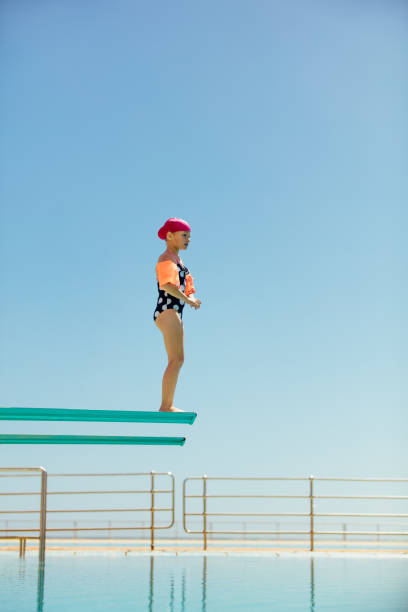
\includegraphics[width=0.25\linewidth]{../figs/D11-4-4}
		\captionof{figure}{Minh hoạ người nhún lên ván để ván dao động.}
	\end{center}
	\begin{enumerate}[label=\alph*)]
		\item Kết quả mô tả ở đề bài liên quan đến hiện tượng vật lý nào mà em đã được học? Điều kiện để xảy ra hiện tượng trên là gì?
		\item Nếu em di chuyển đến giữa tấm ván và lặp lại thí nghiệm như trên thì tần số $f$ sẽ cần phải lớn hơn, nhỏ hơn, hay bằng tần số ban đầu để ván dao động với biên độ cực đại? Em hãy đưa ra giải thích để chứng minh cho câu trả lời của em.
	\end{enumerate}
\hideall{
\begin{enumerate}[label=\alph*)]
	\item Khi người nhún lên tấm ván, người này đã tác dụng ngoại lực tuần hoàn lên ván làm ván dao động cưỡng bức. Khi thay đổi tần số của ngoại lực cưỡng bức đến giá trị bằng tần số dao động riêng của ván thì ván sẽ dao động với biên độ cực đại, đây là hiện tượng cộng hưởng.\\
	Điều kiện xảy ra hiện tượng cộng hưởng là tần số của ngoại lực cưỡng bức tác dụng lên hệ dao động bằng với tần số dao động riêng của hệ.
	\item Khi người nhún lên ván, tấm ván biến dạng đàn hồi và bắt đầu dao động. Ta có thể xem tấm ván như một lò xo có độ cứng $k$. Tần số dao động riêng của hệ ván và người
	$$f=\dfrac{1}{2\pi}\sqrt{\dfrac{k}{m}}$$
	với $m$ là khối lượng của người và ván.\\
	Nhận thấy rằng với cùng trọng lượng của người tác dụng lên ván, khi càng tiến vào gần đầu ván thì độ biến dạng của ván càng giảm, điều đó chứng tỏ rằng độ cứng của ván càng tăng $\left(k=\dfrac{P}{\Delta\ell}\right)$. Do đó, tần số dao động riêng của ván càng tăng khi người này tiến về đầu ván.\\
	Vậy khi người này tiến về phần giữa của ván thì $f$ phải lớn hơn giá trị ban đầu (khi đứng ở cuối ván) để ván dao động với biên độ cực đại.
\end{enumerate}
}
	\item \textbf{\textit{(2,5 điểm)}:}\\
	{Đồ thị li độ - thời gian của một vật dao động điều hoà được thể hiện như hình \ref{fig:4.1}. Dựa vào đồ thị, em hãy xác định
	\begin{center}
		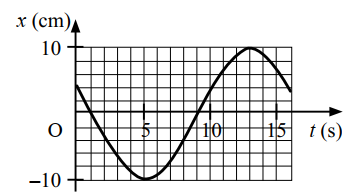
\includegraphics[width=0.45\linewidth]{../figs/D11-4-2}
		\captionof{figure}{Đồ thị li độ - thời gian của vật dao động điều hoà.}
		\label{fig:4.1}
	\end{center}
\begin{enumerate}[label=\alph*)]
	\item Biên độ dao động.
	\item Chu kì dao động.
	\item Tần số góc dao động.
	\item Tốc độ trung bình của vật trong thời gian $\SI{8}{\second}$.
	\item Vận tốc của vật tại thời điểm $t=\SI{12}{\second}$.
\end{enumerate}}
\hideall{
\begin{enumerate}[label=\alph*)]
	\item Biên độ dao động của vật $A=\SI{10}{\centi\meter}$.
	\item Chu kì dao động của vật: $T=\SI{16}{\second}$.
	\item Tần số góc dao động:
	$$\omega=\dfrac{2\pi}{T}=\xsi{\dfrac{\pi}{8}}{\radian/\second}$$
	\item Trong khoảng thời gian $\Delta t=\SI{8}{\second}=\dfrac{T}{2}$ vật đi được quãng đường $s=2A=\SI{20}{\centi\meter}$.\\
	Tốc độ trung bình của vật trong khoảng thời gian này
	$$v_\text{tb}=\dfrac{s}{\Delta t}=\dfrac{\SI{20}{\centi\meter}}{\SI{8}{\second}}=\SI{2.5}{\centi\meter/\second}.$$
	\item Tại thời điểm $t=\SI{5}{\second}$ vật qua vị trí $x=-A$, pha dao động của vật lúc này
	$$\varphi=\omega t+\varphi_0=\xsi{\pi}{\radian}\Rightarrow \varphi_0=\varphi-\omega t=\xsi{\pi}{\radian} -\left(\xsi{\dfrac{\pi}{8}}{\radian/\second}\right)\cdot\left(\SI{5}{\second}\right)=\xsi{\dfrac{3\pi}{8}}{\radian}$$
	Phương trình dao động của vật:
	$$x=A\cos\left(\omega t+\varphi_0\right)=\xsi{10\cos\left(\dfrac{\pi}{8}t+\dfrac{3\pi}{8}\right)}{\centi\meter}$$
	Phương trình vận tốc của vật:
	$$v=-\omega A\sin\left(\omega t+\varphi_0\right)=\xsi{-1,25\pi\sin\left(\dfrac{\pi}{8}t+\dfrac{3\pi}{8}\right)}{\centi\meter/\second}$$
	Tại thời điểm $t=\SI{12}{\second}$ thì vận tốc của vật có giá trị:
	$$v=-1,25\pi\sin\left(\dfrac{\pi}{8}\cdot12+\dfrac{3\pi}{8}\right)\approx\SI{1.5}{\centi\meter/\second}.$$
\end{enumerate}
}
\item \textbf{\textit{(3,0 điểm)}:}\\ {Một xe chạy trên đệm khí được mắc vào lò xo nhẹ có một đầu cố định như hình \ref{fig:4.2}. Khối lượng của xe là $\SI{0.12}{\kilogram}$ và xe dao động với biên độ $\SI{0.075}{\meter}$. Khi qua vị trí cân bằng, xe có tốc độ $\SI{0.524}{\meter/\second}$. Hãy xác định
\begin{center}
	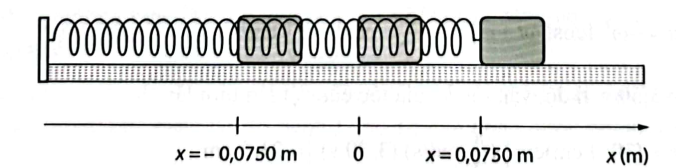
\includegraphics[width=0.7\linewidth]{../figs/D11-4-3}
	\captionof{figure}{Minh hoạ xe chạy trên đệm không khí.}
	\label{fig:4.2}
\end{center}
\begin{enumerate}[label=\alph*)]
	\item Độ cứng của lò xo.
	\item Gia tốc của xe khi nó ở vị trí biên dương.
	\item Cơ năng dao động của xe.
	\item Các vị trí xe có động năng gấp đôi thế năng.
\end{enumerate}}
\hideall{
	\begin{enumerate}[label=\alph*)]
		\item Khi xe qua VTCB, tốc độ của nó đạt cực đại:
		$$v_\text{max}=\omega A\Rightarrow \omega=\dfrac{v_\text{max}}{A}=\dfrac{\SI{0.524}{\meter/\second}}{\SI{0.075}{\meter}}\approx\SI{6.99}{\radian/\second}$$
		Độ cứng của lò xo:
		$$k=m\omega^2=\left(\SI{0.12}{\kilogram}\right)\cdot\left(\SI{6.99}{\radian/\second}\right)^2=\SI{5.86}{\newton/\meter}.$$
		\item Khi xe ở vị trí biên dương, gia tốc của xe:
		$$a=-\omega^2A=-\left(\SI{6.99}{\radian/\second}\right)^2\cdot\left(\SI{0.075}{\meter}\right)=\SI{-3.66}{\meter/\second^2}.$$
		\item Cơ năng của xe:
		$$W=W_\text{đ max}=\dfrac{1}{2}mv^2_\text{max}=\dfrac{1}{2}\cdot\left(\SI{0.12}{\kilogram}\right)\cdot\left(\SI{0.524}{\meter/\second}\right)^2=\SI{0.0165}{\joule}.$$
		\item Khi vật qua vị trí có động năng gấp đôi thế năng $W_\text{đ}=2W_\text{t}$ thì 
		$$W_\text{t}=\dfrac{1}{3}W\Leftrightarrow \dfrac{1}{2}kx^2=\dfrac{1}{3}\cdot\dfrac{1}{2}kA^2$$
		$$\Rightarrow x=\pm\dfrac{A}{\sqrt{3}}\approx\pm\SI{0.0433}{\meter}.$$
	\end{enumerate}
}
\item \textbf{\textit{(3,0 điểm)}:}\\ Một con lắc đơn gồm vật nhỏ khối lượng $\SI{50}{\gram}$ treo vào sợi dây có chiều dài $\SI{2.23}{\meter}$ tại nơi có gia tốc trọng trường $g$. Đồ thị vận tốc - thời gian của vật nhỏ khi con lắc dao động như ở hình \ref{fig:4.3}. Xác định
\begin{center}
	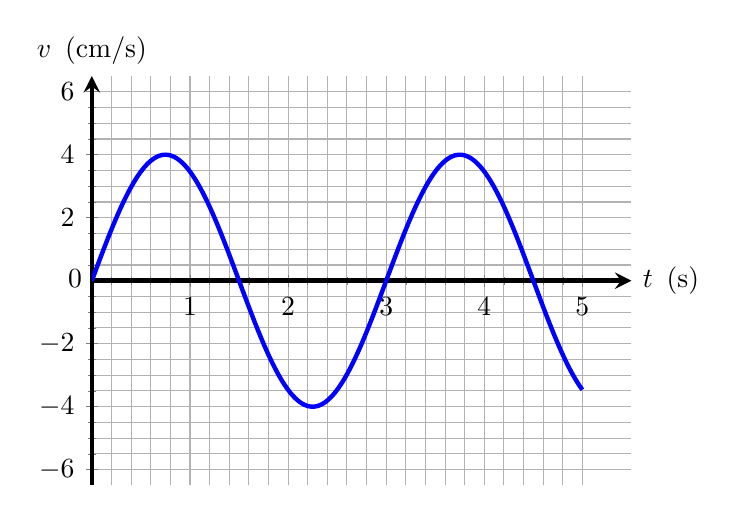
\begin{tikzpicture}  
		\begin{axis}[  ultra thick,
			xmin=0,  
			xmax=5.5,  
			xtick={0,1,...,5},
			ytick={-6,-4,...,6},
			minor x tick num=4,
			minor y tick num=3,
			ymin=-6.5,  
			ymax=6.5, 
			y=0.4cm,
			samples=300,
			axis lines=center, 
			grid style={step=1, color=gray!60!white},
			grid=both,
			xlabel=$t\ \left(\si{\second}\right)$, 
			ylabel=$v\ \left(\si{\centi\meter/\second}\right)$, 
			every axis y label/.style={at=(current axis.above origin),anchor=south},  
			every axis x label/.style={at=(current axis.right of origin),anchor=west},  ]
			\addplot [ultra thick, blue, smooth, domain=0:5] {4*cos(deg(2*pi*x/3-pi/2))}; 
		\end{axis}  
		\node[label={[left]90:0}] at (0,2.5){};
	\end{tikzpicture}
\captionof{figure}{Đồ thị vận tốc - thời gian của con lắc đơn.}
\label{fig:4.3}
\end{center}
\begin{enumerate}[label=\alph*)]
	\item Gia tốc trọng trường tại nơi treo con lắc.
	\item Gia tốc cực đại của vật.
	\item Li độ của vật tại thời điểm $t=\SI{2.0}{\second}$.
	\item Lực căng dây treo khi vật qua vị trí có li độ góc bằng một nửa li độ góc cực đại.
\end{enumerate}
\hideall{
\begin{enumerate}[label=\alph*)]
	\item Chu kì dao động của con lắc $T=\SI{3}{\second}$.\\
	Gia tốc trọng trường tại nơi treo con lắc:
	$$g=\dfrac{4\pi^2\ell}{T^2}=\dfrac{4\pi^2\cdot\left(\SI{2.23}{\meter}\right)}{\left(\SI{3}{\second}\right)^2}\approx\SI{9.78}{\meter/\second^2}.$$
	\item Gia tốc cực đại của vật:
	$$a_\text{max}=\omega v_\text{max}=\left(\dfrac{2\pi}{T}\right)\cdot v_\text{max}=\left(\dfrac{2\pi}{\SI{3}{\second}}\right)\cdot\left(\SI{4}{\centi\meter/\second}\right)\approx\SI{8.38}{\centi\meter/\second^2}.$$
	\item Biên độ dao động của vật:
	$$A=\dfrac{v_\text{max}}{\omega}=\dfrac{v_\text{max}}{\dfrac{2\pi}{T}}=\dfrac{\SI{4}{\centi\meter/\second}}{\dfrac{2\pi}{\SI{3}{\second}}}\approx\SI{1.91}{\centi\meter}$$
	Tại $t=\SI{2.0}{\second}$ thì $v=\SI{-3.5}{\centi\meter/\second}$\\
	Li độ của vật tại thời điểm này:
	$$x=\pm\sqrt{A^2-\dfrac{v^2}{\omega^2}}\approx\pm\SI{0.925}{\centi\meter}.$$
	\item Biên độ góc:
	$$\alpha_0=\dfrac{A}{\ell}=\dfrac{\SI{1.91}{\centi\meter}}{\SI{2.23E2}{\centi\meter}}\approx\SI{8.57E-3}{\radian}$$
	Lực căng dây treo:
	\begin{align*}
		T&=mg\left(3\cos\alpha-2\cos\alpha_0\right)=mg\left(3\cos\dfrac{\alpha_0}{2}-2\cos\alpha_0\right)\\
	 &=\left(\SI{50E-3}{\kilogram}\right)\cdot\left(\SI{9.78}{\meter/\second^2}\right)\cdot\left[3\cos\dfrac{\left(\SI{8.57E-3}{\radian}\right)}{2}-2\cos\left(\SI{8.57E-3}{\radian}\right)\right]\approx\SI{0.49}{\newton}.
	\end{align*} 
\end{enumerate}
}
\end{enumerate}
\begin{center}
	\textbf{--- HẾT ---}
\end{center}
%\chapter{Đề 5}
%\begin{center}
	ĐỀ ÔN TẬP KIỂM TRA GIỮA HỌC KỲ I – MÔN VẬT LÝ 11\\
	Thời gian làm bài: 50 phút \\
	(Không kể thời gian phát đề)\\
\end{center}
\begin{enumerate}[label=\bfseries Câu \arabic*]
	\item \textbf{\textit{(1,0 điểm)}:}\\
	Hệ con lắc lò xo đang dao động điều hoà, nếu người ta tăng khối lượng vật nặng lên gấp đôi và giữ nguyên biên độ dao động của vật nặng thì năng lượng dao động của hệ sẽ thay đổi như thế nào? Sự thay đổi trên sẽ ảnh hưởng như thế nào đến động năng và thế năng của hệ? Em hãy đưa ra giải thích cho kết luận của mình.
	\hideall{
Năng lượng dao động của hệ:
$$W=\dfrac{1}{2}kA^2$$
Vì năng lượng dao động của hệ không phụ thuộc vào khối lượng vật nặng nên khi thay đổi khối lượng vật nặng nhưng vẫn giữ nguyên biên độ dao động của hệ thì năng lượng của hệ không thay đổi.\\
Do đó, động năng cực đại và thế năng cực đại của hệ cũng không đổi. Tuy nhiên, chu kì biến thiên của động năng và thế năng
$$T'=\dfrac{T}{2}=\pi\sqrt{\dfrac{m}{k}}$$
Khi khối lượng của vật nặng tăng gấp đôi thì chu kì biến thiên của động năng và thế năng tăng $\sqrt{2}$ lần.	
}

\item \textbf{\textit{(1,0 điểm)}:}\\
Con lắc đơn tạo bởi quả cầu rỗng, bên trong chứa đầy nước được treo ở đầu sợi dây nhẹ, không dãn. Con lắc dao động điều hoà trong môi trường không có lực cản. Nếu bên dưới quả cầu có một lỗ nhỏ và nước có thể chảy từ từ ra khỏi quả cầu từ lỗ trống này thì chu kì dao động của con lắc sẽ thay đổi như thế nào? Em hãy đưa ra giải thích cho kết luận của mình.
\hideall{
Chu kì dao động của con lắc đơn
$$T=2\pi\sqrt{\dfrac{\ell}{g}}$$
$\ell$ là khoảng cách từ điểm treo đến khối tâm của vật nặng.\\
Khi nước chảy ra ngoài quả cầu, khối tâm của quả cầu bị hạ thấp dần do đó $\ell$ tăng lên. Như vậy, chu kì dao động của con lắc sẽ tăng lên.\\
Khi toàn bộ nước chảy ra ngoài, khối tâm quả cầu trở về vị trí ban đầu, chu kì dao động của con lắc bằng chu kì dao động ban đầu.
}

\item \textbf{\textit{(3,0 điểm)}:}\\
Một lò xo có khối lượng không đáng kể bị kéo dãn $\SI{3.0}{\centi\meter}$ nếu chịu tác dụng của lực có độ lớn $\SI{7.5}{\newton}$ tác dụng dọc theo trục lò xo. Vật nhỏ khối lượng $\SI{0.5}{\kilogram}$ nằm trên mặt phẳng nằm ngang không ma sát và được gắn vào đầu tự do của lò xo. Người ta kéo vật nặng đến vị trí lò xo dãn $\SI{5}{\centi\meter}$ rồi thả nhẹ cho vật dao động.
\begin{enumerate}[label=\alph*)]
	\item Độ cứng của lò xo là bao nhiêu?
	\item Tính tần số góc dao động của vật.
	\item Xác định độ dịch chuyển của vật so với vị trí cân bằng tại thời điểm $t=\SI{0.5}{\second}.$
	\item Xác định vận tốc và gia tốc của vật tại thời điểm $t=\SI{0.5}{\second}.$
\end{enumerate}
\hideall{
\begin{enumerate}[label=\alph*)]
	\item Độ cứng của lò xo:
	$$k=\dfrac{F}{\Delta\ell}=\dfrac{\SI{7.5}{\newton}}{\SI{3E-2}{\centi\meter}}=\SI{250}{\newton\meter}.$$
	\item Tần số góc dao động của vật:
	$$\omega=\sqrt{\dfrac{k}{m}}=\sqrt{\dfrac{\SI{250}{\newton/\meter}}{\SI{0.5}{\kilogram}}}=\xsi{10\sqrt{5}}{\radian/\second}.$$
	\item Chọn gốc thời gian lúc thả vật, chiều dương cùng chiều biến dạng ban đầu của lò xo.\\
	Phương trình dao động của vật:
	$$x=A\cos\left(\omega t+\varphi_0\right)=\xsi{5\cos\left(10\sqrt{5}t\right)}{\centi\meter}$$
	Tại thời điểm $t=\SI{0.5}{\second}$ thì $x\approx\SI{0.92}{\centi\meter}.$
	\item Phương trình vận tốc của vật:
	$$v=-\omega A\sin\left(\omega t+\varphi_0\right)=\xsi{-50\sqrt{5}\sin\left(10\sqrt{5}t\right)}{\centi\meter/\second}$$
	Tại thời điểm $t=\SI{0.5}{\second}$ thì $v\approx\SI{109.9}{\centi\meter/\second}.$\\
	Gia tốc của vật:
	$$a=-\omega^2x=-\left(\xsi{10\sqrt{5}}{\radian/\second}\right)^2\cdot\left(\SI{0.92}{\centi\meter}\right)=-\SI{460}{\centi\meter/\second^2}.$$
\end{enumerate}
}

	\item \textbf{\textit{(3,0 điểm)}:}\\
	Một con lắc đơn gồm sợi dây có chiều dài $\SI{1.20}{\meter}$ và vật nặng có khối lượng $\SI{0.5}{\kilogram}$. Treo con lắc tại nơi có gia tốc trọng trường $\SI{9.81}{\meter/\second^2}$. Kéo vật ra khỏi vị trí cân bằng sao cho sợi dây tạo với phương thẳng đứng một góc $\alpha_0$ rồi thả tay cho vật dao động không vận tốc đầu. Bỏ qua mọi lực cản. Tính tốc độ của vật khi nó qua vị trí cân bằng và độ lớn lực căng của dây treo khi đó trong trường hợp:
	\begin{enumerate}[label=\alph*)]
		\item $\alpha_0=\SI{8.0}{\degree}$.
		\item $\alpha_0=\SI{30.0}{\degree}$.
	\end{enumerate}
\hideall{
\begin{enumerate}[label=\alph*)]
	\item Khi góc $\alpha_0=\SI{8}{\degree}=\SI{0.14}{\radian}$, con lắc dao động với biên độ nhỏ nên được coi là dao động điều hoà với tần số góc:
	$$\omega=\sqrt{\dfrac{g}{\ell}}\approx\SI{2.86}{\radian/\second}$$
	Biên độ dao động của con lắc:
	$$A=\alpha_0\ell=\SI{0.168}{\meter}$$
	Tốc độ của vật khi đi qua vị trí cân bằng:
	$$v_\text{max}=\omega A=\SI{0.48}{\meter/\second}.$$
	Ở vị trí cân bằng, tổng hợp trọng lực và lực căng dây treo tác dụng lên vật đóng vai trò là lực hướng tâm:
	$$T-P=F_\text{ht}=\dfrac{mv^2_\text{max}}{\ell}\Rightarrow T=mg+\dfrac{mv^2_\text{max}}{\ell}=\SI{5.0}{\newton}.$$
	\item Khi $\alpha_0=\SI{30}{\degree}$, dao động của con lắc đơn không phải là dao động điều hoà.
	\begin{center}
		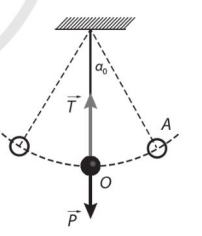
\includegraphics[width=0.3\linewidth]{../figs/D11-5-1}
	\end{center}
	Chọn gốc thế năng hấp dẫn tại vị trí cân bằng của vật nặng, áp dụng định luật bảo toàn cơ năng cho chuyển động của con lắc đơn ở môi trường không có lực cản:
	$$W_\text{O}=W_\text{A}\Leftrightarrow \dfrac{1}{2}mv^2_\text{max}=mg\ell\left(1-\cos\alpha_0\right)$$
	$$\Leftrightarrow v_\text{max}=\sqrt{2g\ell\left(1-\cos\alpha_0\right)}=\SI{1.78}{\meter/\second}$$
	Lực căng dây treo:
	$$T=mg+\dfrac{mv^2_\text{max}}{\ell}=\SI{6.23}{\newton}.$$
\end{enumerate}
}

\item \textbf{\textit{(1,0 điểm)}:}\\
Một con lắc lò xo đang dao động tắt dần với cơ năng ban đầu của nó là $\SI{10}{\joule}$, sau ba chu kì dao động biên độ của nó giảm $\SI{10}{\percent}$. Phần cơ năng chuyển hoá thành nhiệt sau khoảng thời gian đó bằng bao nhiêu?
\hideall{
Gọi $A$ là biên độ dao động ban đầu của vật nặng, cơ năng ban đầu của vật
$$W=\dfrac{1}{2}kA^2=\SI{10}{\joule}$$
Sau 3 chu kì dao động $A'=0,9A$
$$\Rightarrow W'=\dfrac{1}{2}kA'^2=0,81\cdot\dfrac{1}{2}kA^2=\SI{8.1}{\joule}$$
Phần cơ năng chuyển hoá thành nhiệt:
$$\Delta W=W-W'=\SI{1.9}{\joule}.$$
}

\item \textbf{\textit{(1,0 điểm)}:}\\
Một chiếc xe máy chạy trên một con đường lát gạch, cứ cách khoảng $\SI{4}{\meter}$ trên đường lại có một cái rãnh nhỏ. Chu kì dao động riêng của khung xe máy trên các lò xo giảm xóc là $\SI{0.5}{\second}$. Xe bị xóc mạnh nhất khi chuyển động với tốc độ bằng bao nhiêu?
\hideall{
	Xe bị xóc mạnh nhất khi chu kì ngoại lực kích thích bằng chu kì dao động riêng của khung xe $T=T_0=\SI{4}{\second}$.\\
	Tốc độ của xe khi xe xóc mạnh nhất:
	$$v=\dfrac{s}{T}=\SI{8}{\meter/\second}.$$
}
\end{enumerate}
%\chapter{Đề 6}
%\begin{center}
	ĐỀ ÔN TẬP KIỂM TRA GIỮA HỌC KỲ I – MÔN VẬT LÝ 11\\
	Thời gian làm bài: 50 phút \\
	(Không kể thời gian phát đề)\\
\end{center}
\ANSMCQ{
	\begin{center}
		\begin{tabular}{|m{2.8em}|m{2.8em}|m{2.8em}|m{2.8em}|m{2.8em}|m{2.8em}|m{2.8em}|m{2.8em}|m{2.8em}|m{2.8em}|}
			\hline
			1D & 2D & 3B & 4A & 5D & 6C & 7C & 8A & 9D & 10A\\
			\hline
			11D & 12A & 13D & 14C & 15D & 16B & 17C & 18B & 19B & 20B\\
			\hline
			21C & 22BC & 23C & 24D & 25B & 26C & 27C & 28B & 29D & 30C\\
			\hline
		\end{tabular}
\end{center}}
\begin{enumerate}[label=\bfseries Câu \arabic*:]
	\item Đại lương cho biết số dao động mà vật thực hiện được trong $\SI{1}{\second}$ gọi là
	\begin{mcq}(4)
		\item pha dao động.
		\item tần số góc.
		\item biên độ.
		\item li độ.
	\end{mcq}
	\hideall{
		\textbf{Đáp án B.}
	}
	
	\item Trong dao động điều hòa thì nhóm đại lượng nào sau đây không thay đổi theo thời gian?
	\begin{mcq}(2)
		\item Li độ và thời gian.
		\item Biên độ và tần số góc.
		\item Li độ và pha ban đầu.
		\item Tần số và pha dao động.
	\end{mcq}
	\hideall{
		\textbf{Đáp án B.}
	}
	
	\item Một chất điểm dao động điều hoà với phương trình $x=\xsi{10\cos\left(15t+\pi\right)}{\centi\meter}$ ($x$ tính bằng $\si{\centi\meter}$, $t$ tính bằng giây). Chất điểm này dao động với tần số góc là
	\begin{mcq}(4)
		\item $\SI{20}{\radian/\second}$.
		\item $\SI{10}{\radian/\second}$.
		\item $\SI{5}{\radian/\second}$.
		\item $\SI{15}{\radian/\second}$.
	\end{mcq}
	\hideall{
		\textbf{Đáp án D.}
	}
	
	\item Một chất điểm chuyển động tròn đều trên một đường tròn bán kính $R$, tốc độ góc $\omega
	$. Hình chiếu của chất điểm này lên đường kính là một dao động điều hoà có
	\begin{mcq}(2)
		\item biên độ $R$.
		\item biên độ $2R$.
		\item pha ban đầu $\omega t$.
		\item chiều dài quỹ đạo $4R$.
	\end{mcq}
	\hideall{
		\textbf{Đáp án D.}
	}
	
	\item Một chất điểm dao động điều hoà với phương trình $x=\xsi{5\cos\left(10\pi t+\dfrac{\pi}{3}\right)}{\centi\meter}$. Li độ của vật khi pha dao động bằng $\xsi{\pi}{\radian}$ là
	\begin{mcq}(4)
		\item $\SI{5}{\centi\meter}$.
		\item $\SI{-5}{\centi\meter}$.
		\item $\SI{2.5}{\centi\meter}$.
		\item $\SI{-2.4}{\centi\meter}.$
	\end{mcq}
	\hideall{
		\textbf{Đáp án B.}\\
		Khi pha dao động là $\varphi=\xsi{\pi}{\radian}$ thì li độ dao động của vật là
		$$x=5\cos\pi=-\SI{5}{\centi\meter}.$$
	}
	
	\item Một chất điểm dao động điều hòa trong 10 dao động toàn phần đi được quãng đường $\SI{120}{\centi\meter}$. Quỹ đạo của dao động có chiều dài là
	\begin{mcq}(4)
		\item $\SI{6}{\centi\meter}$.
		\item $\SI{12}{\centi\meter}$.
		\item $\SI{3}{\centi\meter}$.
		\item $\SI{9}{\centi\meter}$.
	\end{mcq}
	\hideall{
		\textbf{Đáp án C.}\\
		Biên độ dao động của chất điểm:
		$$A=\dfrac{s}{4\cdot10}=\SI{3}{\centi\meter}$$
		Chiều dài quỹ đạo:
		$$L=2A=\SI{6}{\centi\meter}.$$
	}
	
	\item Trong một trò chơi bắn súng, một khẩu súng bắn vào mục tiêu di động. Súng tự nhả đạn theo thời gian một cách ngẫu nhiên. Người chơi phải chĩa súng theo một hướng nhất định còn mục tiêu dao động điều hoà theo phương ngang như hình vẽ. Người chơi cần chĩa súng vào vùng nào để có thể ghi được số lần trúng nhiều nhất?
	\begin{center}
		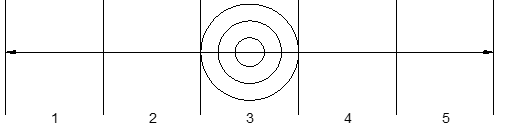
\includegraphics[width=0.5\linewidth]{../figs/D11-4-1}
	\end{center}
	\begin{mcq}(2)
		\item vùng 3.
		\item vùng 1 hoặc vùng 5.
		\item vùng 2 hoặc 4.
		\item bất kì vùng nào.
	\end{mcq}
	\hideall{
		\textbf{Đáp án B.}\\
		Tốc độ của vật ở vị trí biên là nhỏ nhất, thời gian vật ở vùng 1 và vùng 5 cũng lớn hơn so với các vùng khác nên xác suất ghi điểm ở vùng 1 và 5 là cao nhất.
	}
	
	\item Một vật dao động điều hoà phải mất $\SI{0.025}{\second}$ để đi từ điểm có vận tốc bằng không đến điểm tiếp theo cũng có vận tốc bằng không, hai điểm ấy cách nhau $\SI{10}{\centi\meter}$. Chọn phát biểu đúng.
	\begin{mcq}(4)
		\item Chu kì dao động là $\SI{0.025}{\second}$.
		\item Tần số dao động là $\SI{10}{\hertz}$.
		\item Biên độ dao động là $\SI{10}{\centi\meter}$.
		\item Vận tốc của vật có độ lớn cực đại là $\xsi{2\pi}{\meter/\second}$.
	\end{mcq}
	\hideall{
		\textbf{Đáp án D.}\\
		Vật có vận tốc bằng 0 khi ở vị trí biên. Như vậy ta có
		$$\dfrac{T}{2}=\SI{0.025}{\second}\Rightarrow T=\SI{0.05}{\second};\quad A=\SI{5}{\centi\meter}$$
		Vận tốc cực đại của vật:
		$$v_\text{max}=\omega A=\dfrac{2\pi}{T}\cdot A=\dfrac{2\pi}{\SI{0.05}{\second}}\cdot\left(\SI{0.05}{\meter}\right)=\xsi{2\pi}{\meter/\second}.$$
	}
	
	\item Một vật dao động điều hoà với phương trình li độ $x=A\cos\left(\omega t+\varphi_0\right)$. Gọi $v$ là vận tốc của vật khi vật ở vị trí li độ $x$. Biên độ dao động của vật là
	\begin{mcq}(4)
		\item $\sqrt{x^2+\dfrac{v^4}{\omega^2}}$.
		\item $\sqrt{x^2+\dfrac{v^2}{\omega^2}}$>
		\item $\sqrt{x^2+\dfrac{v^2}{\omega^4}}$.
		\item $\sqrt{x+\dfrac{v^2}{\omega^2}}$.
	\end{mcq}
	\hideall{
		\textbf{Đáp án B.}
	}
	
	\item Một chất điểm dao động điều hoà với tần số bằng $\SI{4}{\hertz}$ và biên độ bằng $\SI{10}{\centi\meter}$. Gia tốc cực đại của chất điểm bằng
	\begin{mcq}(4)
		\item $\SI{25}{\centi\meter/\second^2}$.
		\item $\SI{2.5}{\meter/\second^2}$.
		\item $\SI{63.2}{\meter/\second}$.
		\item $\SI{6.32}{\meter/\second^2}$.
	\end{mcq}
	\hideall{
		\textbf{Đáp án C.}\\
		Gia tốc cực đại của vật là
		$$a_\text{max}=\omega^2 A=\left(2\pi f\right)^2A\approx\SI{63.2}{\meter/\second^2}.$$
	}
	
	\item Một chất điểm dao động điều hoà có phương trình vận tốc $v=\xsi{20\pi \cos\left(2\pi t+\dfrac{\pi}{6}\right)}{\centi\meter/\second}$. Phương trình dao động của chất điểm có dạng 
	\begin{mcq}(2)
		\item $x=\xsi{10\cos\left(2\pi t-\dfrac{\pi}{3}\right)}{\centi\meter}.$
		\item $x=\xsi{10\cos\left(2\pi t+\dfrac{2\pi}{3}\right)}{\centi\meter}.$
		\item $x=\xsi{20\cos\left(2\pi t+\dfrac{5\pi}{6}\right)}{\centi\meter}.$
		\item $x=\xsi{20\cos\left(2\pi t+\dfrac{\pi}{3}\right)}{\centi\meter}.$
	\end{mcq}
	\hideall{
		\textbf{Đáp án A.}\\
		Biên độ dao động của chất điểm:
		$$A=\dfrac{v_\text{max}}{\omega}=\SI{10}{\centi\meter}.$$
		Pha ban đầu của dao động:
		$$\varphi_{0x}=\varphi_{0v}-\dfrac{\pi}{2}=-\xsi{\dfrac{\pi}{3}}{\radian}$$
		Phương trình li độ của chất điểm:
		$$x=\xsi{10\cos\left(2\pi t-\dfrac{\pi}{3}\right)}{\centi\meter}.$$
	}
	
	\item Một chất điểm dao động điều hoà trên trục $Ox$. Tại thời điểm $t_1$, $t_2$ vật có vận tốc và gia tốc lần lượt là $v_1=\xsi{10\sqrt{3}}{\centi\meter/\second}$; $a_1=\SI{-1}{\meter/\second^2}$; $v_2=\SI{-10}{\centi\meter/\second}$; $a_2=\xsi{\sqrt{3}}{\meter/\second^2}$. Tốc độ cực đại của vật bằng
	\begin{mcq}(4)
		\item $\SI{20}{\centi\meter/\second}$.
		\item $\SI{40}{\centi\meter/\second}$.
		\item $\xsi{10\sqrt{5}}{\centi\meter/\second}$.
		\item $\xsi{20\sqrt{3}}{\centi\meter/\second}.$
	\end{mcq}
	\hideall{
		\textbf{Đáp án A.}\\
		Áp dụng hệ thức độc lập thời gian
		$$\dfrac{v^2}{v^2_\text{max}}+\dfrac{a^2}{a^2_\text{max}}=1\Rightarrow\dfrac{1}{a^2_\text{max}}=\dfrac{1-\dfrac{v^2}{v^2_\text{max}}}{a^2}$$
		Như vậy:
		$$\dfrac{1-\dfrac{v^2_1}{v^2_\text{max}}}{a^2_1}=\dfrac{1-\dfrac{v^2_2}{v^2_\text{max}}}{a^2_2}\Rightarrow v_\text{max}=\SI{20}{\centi\meter/\second}.$$
	}
\end{enumerate}
% ==================================LỚP 12 =================================================
%	\setcounter{part}{0}
%	\part{TỔNG HỢP KIẾN THỨC}
%	\startcontents[parts]
%	\printcontents[parts]{}{0}{\setcounter{tocdepth}{0}}
%	\setcounter{mychapter}{0}
%	\mychapter{VẬT LÍ NHIỆT}
%	\startcontents[mychapters]
%	\printcontents[mychapters]{}{0}{\setcounter{tocdepth}{1}}
%	\begin{center}
%			
\includegraphics[width=0.8\linewidth]{../figs/G12C1}
%		\end{center}
%	\chapter{Tóm tắt lý thuyết}
\section{Mô hình động học phân tử và sự chuyển thể}
\subsection{Mô hình động học phân tử}
\begin{itemize}
	\item Vật chất được cấu tạo từ các hạt riêng biệt gọi là phân tử.
	\item Các phân tử chuyển động hỗn loạn không ngừng, gọi là chuyển động nhiệt. Nhiệt độ càng cao thì tốc độ trung bình của các phân tử càng lớn.
	\item Giữa các phân tử có lực liên kết phân tử (hút và đẩy).
\end{itemize}
\subsection{Cấu trúc của vật chất}
\begin{center}
	\begin{tabular}{|L{4cm}|L{4cm}|L{4cm}|L{4cm}|}
		\hline
		\thead{Cấu trúc}&\thead{Thể khí}& \thead{Thể rắn}&\thead{Thể lỏng}\\
		\hline
		Khoảng cách giữa các phân tử & Rất xa nhau (gấp hàng chục lần kích thước phân tử) & Rất gần nhau (cỡ kích thước phân tử) & Xa nhau\\
		\hline
		Sự sắp xếp của các phân tử & 	Không có trật tự & Trật tự & Kém trật tự hơn thể rắn\\
		\hline
		Chuyển động của các phân tử & Chuyển động hỗn loạn & Chỉ dao động quanh vị trí cân bằng cố định & Dao động quanh vị trí cân bằng luôn thay đổi\\
		\hline
		Minh họa chuyển động của các phân tử & \begin{center}
			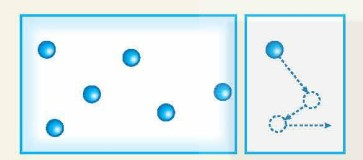
\includegraphics[width=0.8\linewidth]{../figs/G12C1-1}
		\end{center}&\begin{center}
		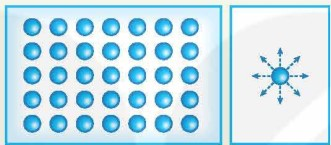
\includegraphics[width=0.8\linewidth]{../figs/G12C1-2}
		\end{center}(Chất rắn kết tinh) &\begin{center}
		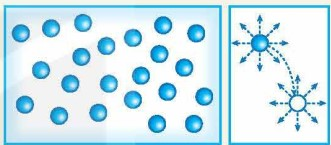
\includegraphics[width=0.8\linewidth]{../figs/G12C1-3}
		\end{center}\\
		\hline
	\end{tabular}
\end{center}
\subsection{Các quá trình chuyển thể}
\begin{itemize}
	\item Các chất có thể chuyển từ thể này sang thể khác.
	\item Cấu trúc của chất thay đổi khi chuyển thể.
\end{itemize}
\begin{center}
	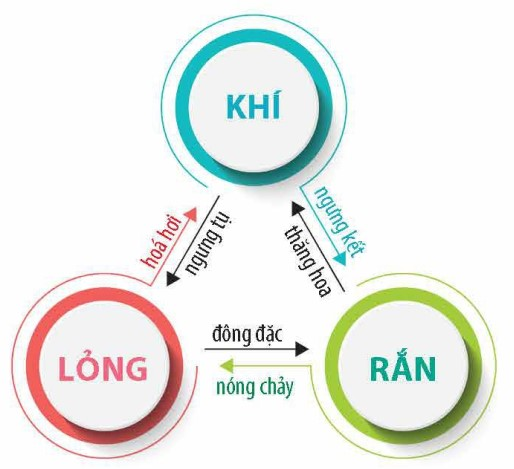
\includegraphics[width=0.35\linewidth]{../figs/G12C1-4}
\end{center}
\luuy{Sự hóa hơi thể hiện qua hai hình thức: sự bay hơi và sự sôi
\begin{itemize}
	\item Sự bay hơi là sự hóa hơi xảy ra trên bề mặt chất lỏng. Sự bay hơi xảy ra ở bất kì nhiệt độ nào.
	\item Sự sôi là sự hóa hơi xảy ra ở bên trong và trên bề mặt chất lỏng. Sự sôi xảy ra ở nhiệt độ sôi.
	\end{itemize}}
\section{Nội năng - Định luật I nhiệt động lực học}
\subsection{Nội năng}
\begin{itemize}
	\item Nội năng của một vật là tổng động năng và thế năng tương tác của các phân tử cấu tạo nên vật.
	\item Nội năng được kí hiệu là $U$ và có đơn vị là $\si{\joule}$.
	\item Nội năng của vật phụ thuộc vào nhiệt độ $T$ và thể tích $V$ của vật.
	\item Có thể làm thay đổi nội năng của vật bằng cách: thực hiện công, truyền nhiệt.
\end{itemize}
\subsection{Định luật I nhiệt động lực học}
Độ biến thiên nội năng của vật bằng tổng công và nhiệt lượng mà vật nhận được.
\begin{equation}
	\Delta U=Q+A
\end{equation}
\begin{center}
	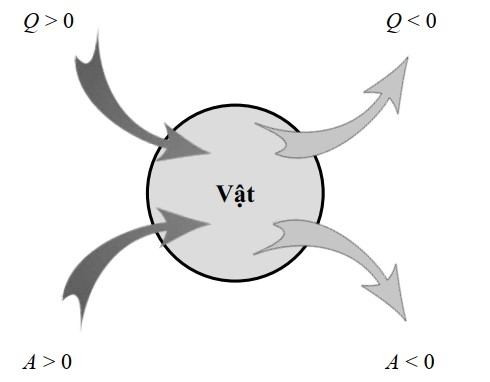
\includegraphics[width=0.3\linewidth]{../figs/G12C1-5}
\end{center}
\section{Thang nhiệt độ}
\subsection{Chiều truyền năng lượng nhiệt giữa hai vật chênh lệch nhiệt độ tiếp xúc nhau}
\begin{itemize}
	\item Khi hai vật chênh lệch nhiệt độ tiếp xúc nhau, năng lượng nhiệt luôn truyền từ vật có nhiệt độ cao hơn sang vật có nhiệt độ thấp hơn.
	\item Quá trình truyền nhiệt kết thúc khi hai vật ở cùng một nhiệt độ (cân bằng nhiệt với nhau).
\end{itemize}
\subsection{Các thang nhiệt độ}
\begin{itemize}
	\item \textit{Thang nhiệt độ Celsius}: Nhiệt độ đóng băng của nước tinh khiết là $\SI{0}{\celsius}$ và nhiệt độ sôi của nước tinh khiết là $\SI{100}{\celsius}$ ở áp suất tiêu chuẩn. Nhiệt độ trong thang Celsius thường được kí hiệu là $t$.
	\item \textit{Thang nhiệt độ Kelvin}: Nhiệt độ thấp nhất mà các vật có thể có được là $\SI{0}{\kelvin}$ (độ không tuyệt đối) và nhiệt độ mà nước tinh khiết có thể tồn tại đồng thời ở cả ba thể rắn, lỏng và hơi là $\SI{273.16}{\kelvin}$. Nhiệt độ trong thang Kelvin thường được kí hiệu là $T$.
	\begin{equation}
		\xsi{T}{\left(\si{\kelvin}\right)}=\xsi{t}{\left(\si{\celsius}\right)}+273
	\end{equation}
	
\end{itemize}
\manatip{Công thức chuyển đổi thang nhiệt độ $X$ sang thang nhiệt độ $Z$ có nhiệt độ đóng băng và nhiệt độ sôi  của nước tinh khiết lần lượt là $\left(X_b,X_s\right)$, $\left(Z_b, Z_s\right)$ trong trường hợp 2 thang nhiệt độ quan hệ tuyến tính với nhau:
	\begin{equation}
		\dfrac{X-X_b}{X_s-X_b}=\dfrac{Y-Y_b}{Y_s-Y_b}
	\end{equation}
	
}
\subsection{Nhiệt độ không tuyệt đối}
Nhiệt độ không tuyệt đối $\left(\SI{0}{\kelvin}\right)$ là nhiệt độ mà tại đó tất cả các chất có động năng chuyển động nhiệt của các phân tử hoặc nguyên tử bằng không và thế năng của chúng là tối thiểu.
\section{Nhiệt dung riêng, nhiệt nóng chảy riêng, nhiệt hóa hơi riêng}
\subsection{Nhiệt dung riêng}
\begin{itemize}
	\item Nhiệt dung riêng của một chất có giá trị bằng nhiệt lượng cần cung cấp để làm tăng nhiệt độ của $\SI{1}{\kilogram}$ chất đó lên $\SI{1}{\kelvin}$.
	\begin{equation}
		c=\dfrac{Q}{m\left(T_2-T_1\right)}
	\end{equation}
	\item Trong hệ SI, đơn vị đo nhiệt dung riêng là $\si{\joule/\left(\kilogram\cdot\kelvin\right)}$.
\end{itemize}
Nhiệt lượng mà một vật có khối lượng $m$ trao đổi khi thay đổi nhiệt độ từ $T_1$ đến $T_2$ được xác định bởi biểu thức: $Q = mc\left(T_2 – T_1\right)$\\
Trong hệ SI, đơn vị đo nhiệt lượng là $\si{\joule}$. Ngoài ra, nhiệt lượng còn được đo bằng đơn vị $\si{cal}$
$$\SI{1}{cal}=\SI{4,186}{\joule}.$$
\subsection{Nhiệt nóng chảy riêng}
\begin{itemize}
	\item Nhiệt nóng chảy riêng của một chất có giá trị bằng nhiệt lượng cần cung cấp cho $\SI{1}{\kilogram}$ chất đó chuyển hoàn toàn từ thể rắn sang thể lỏng tại nhiệt độ nóng chảy.\\
	\begin{equation}
		\lambda=\dfrac{Q}{m}
	\end{equation}
	\item Trong hệ SI, đơn vị đo nhiệt nóng chảy riêng là $\si{\joule/\kilo}$.
\end{itemize}
\subsection{Nhiệt hóa hơi riêng}
\begin{itemize}
	\item Nhiệt hoá hơi riêng của một chất lỏng có giá trị bằng nhiệt lượng cần cung cấp cho $\SI{1}{\kilogram}$ chất lỏng đó hoá hơi hoàn toàn ở nhiệt độ sôi.
	\begin{equation}
		L=\dfrac{Q}{m}
	\end{equation}
	\item Trong hệ SI, đơn vị đo nhiệt hoá hơi riêng là $\si{\joule/\kilogram}$.
\end{itemize}

%	\chapter{Câu hỏi ôn tập}
\hideall{
	\setcounter{section}{0}
	\begin{center}
		\textbf{\large BẢNG ĐÁP ÁN}
	\end{center}
	\section{Câu trắc nghiệm nhiều phương án lựa chọn}
	\inputansbox{10}{ans/Y24-VN12-PH-C1-TN}
	\section{Câu trắc nghiệm đúng sai}
	\inputansbox[2]{2}{ans/Y24-VN12-PH-C1-TF}
	\section{Câu trắc nghiệm trả lời ngắn}
	\inputansbox[3]{6}{ans/Y24-VN12-PH-C1-TL}
}
\setcounter{section}{0}
\section{Câu trắc nghiệm nhiều phương án lựa chọn}
\textit{Thí sinh trả lời từ câu 1 đến câu 18. Mỗi câu thí sinh chọn một phương án}
\setcounter{ex}{0}
\Opensolutionfile{ans}[ans/Y24-VN12-PH-C1-TN]
% ===================================================================
\begin{ex}
	Chất rắn vô định hình là chất rắn
	\choice
	{có cấu trúc tinh thể}
	{\True không có cấu trúc tinh thể}
	{có nhiệt độ nóng chảy xác định}
	{có thể tích thay đổi}
	\loigiai{}
\end{ex}
% ===================================================================
\begin{ex}
	Tính chất nào sau đây \textbf{không phải} là tính chất của các phân tử khí?
	\choice
	{Có vận tốc trung bình phụ thuộc vào nhiệt độ}
	{Gây áp suất lên thành bình}
	{\True Chuyển động xung quanh vị trí cân bằng}
	{Chuyển động nhiệt hỗn loạn}
	\loigiai{}
\end{ex}
% ===================================================================
\begin{ex}
	Sự bay hơi
	\choice
	{\True xảy ra ở bất kì nhiệt độ nào của chất lỏng}
	{chỉ xảy ra ở trong lòng chất lỏng}
	{xảy ra với tốc độ như nhau ở mọi nhiệt độ}
	{chỉ xảy ra đối với một số ít chất lỏng}
	\loigiai{}
\end{ex}
% ===================================================================
\begin{ex}
	Đơn vị của nhiệt dung riêng là
		\choice
	{$\si{\joule/\kilogram}$}
	{$\si{\kilogram/\joule}$}
	{\True $\si{\joule/\kilogram\cdot\kelvin}$}
	{$\si{\kilogram/\joule\cdot\kelvin}$}
	\loigiai{}
\end{ex}
% ===================================================================
\begin{ex}
	Phát biểu nào sau đây là \textbf{sai}?
	\choice
	{Nhiệt độ sôi của chất lỏng phụ thuộc vào áp suất khí phía trên bề mặt chất lỏng}
	{Áp suất khí càng cao thì nhiệt độ sôi của chất lỏng càng cao}
	{\True Áp suất khí càng nhỏ thì nhiệt độ sôi của chất lỏng càng cao.}
	{Ở một áp suất nhất định, mỗi chất lỏng sôi ở nhiệt độ xác định và không đổi}
	\loigiai{}
\end{ex}
% ===================================================================
\begin{ex}
Nội năng của một vật là	
	\choice
	{tổng động năng chuyển động nhiệt của các phân tử cấu tạo nên vật}
	{\True tổng động năng và thế năng của các phân tử cấu tạo nên vật}
	{tổng nhiệt năng và cơ năng mà vật nhận được trong quá trình truyền nhiệt và thực hiện công}
	{nhiệt lượng vật nhận được trong quá trình truyền nhiệt}
	\loigiai{}
\end{ex}
% ===================================================================
\begin{ex}
	Nhiệt hóa hơi riêng của một chất lỏng là nhiệt lượng cần thiết để
	\choice
	{\True làm cho một kilogram chất lỏng đó hóa hơi hoàn toàn ở nhiệt độ xác định}
	{làm cho một kilogram chất lỏng tăng thêm $\SI{1}{\celsius}$}
	{làm cho một khối lượng xác định chất lỏng đó hóa hơi hoàn toàn}
	{làm cho một kilogram hơi chuyển hoàn toàn sang thể lỏng ở nhiệt độ xác định}
	\loigiai{}
\end{ex}
% ===================================================================
\begin{ex}
	Người ta thực hiện công $\SI{40}{\joule}$ lên khối khí trong xi lanh làm cho nội năng khối khí tăng thêm $\SI{20}{\joule}$ thì khối khí
	\choice
	{\True tỏa nhiệt $\SI{20}{\joule}$}
	{nhận nhiệt $\SI{20}{\joule}$}
	{tỏa nhiệt $\SI{40}{\joule}$}
	{nhận nhiệt $\SI{40}{\joule}$}
	\loigiai{}
\end{ex}
% ===================================================================
\begin{ex}
	Không thể dùng nhiệt kế rượu để đo nhiệt độ của nước đang sôi vì
	\choice
	{rượu sôi ở nhiệt độ cao hơn $\SI{100}{\celsius}$}
	{\True rượu sôi ở nhiệt độ thấp hơn $\SI{100}{\celsius}$}
	{rượu đông đặc ở nhiệt độ cao hơn $\SI{100}{\celsius}$}
	{rượu đông đặc ở nhiệt độ thấp hơn $\SI{0}{\celsius}$}
	\loigiai{}
\end{ex}
% ===================================================================
\begin{ex}
	Nhiệt độ trung bình trong 1 căn phòng ở thang nhiệt độ Celsius là $\SI{27}{\celsius}$. Nhiệt độ này trong thang nhiệt độ Kelvin là
	\choice
	{$\SI{273}{\kelvin}$}
	{\True $\SI{300}{\kelvin}$}
	{$\SI{246}{\kelvin}$}
	{$\SI{327}{\kelvin}$}
	\loigiai{}
\end{ex}
% ===================================================================
\begin{ex}
	Người ta bỏ $\SI{100}{\gram}$ nước đá ở $\SI{0}{\celsius}$ vào $\SI{300}{\gram}$ nước có nhiệt độ $\SI{30}{\celsius}$. Cho biết nhiệt nóng chảy riêng của nước đá $\lambda=\SI{3.4e5}{\joule/\kilogram}$ và nhiệt dung riêng của nước là $c =\SI{4200}{\joule/\left(\kilogram\cdot\kelvin\right)}$. Lượng nước đá còn lại chưa tan hết là
	\choice
	{$\SI{26}{\gram}$}
	{$\SI{74}{\gram}$}
	{$\SI{35}{\gram}$}
	{\True $\SI{0}{\gram}$}
	\loigiai{
	Lượng nước đá có thể tan nếu nhận nhiệt lượng do $\SI{300}{\gram}$ nước tỏa ra khi giảm nhiệt độ từ $\SI{30}{\celsius}$ xuống $\SI{0}{\celsius}$:
	$$m=\dfrac{m_nct_0}{\lambda}\approx\SI{111.12}{\gram}.$$
	}
\end{ex}
% ===================================================================
\begin{ex}
Biết nhiệt dung riêng và nhiệt nóng chảy riêng của đồng lần lượt là $c =\SI{380}{\joule/\left(\kilogram\cdot\kelvin\right)}$; $\lambda =\SI{180}{\kilo\joule/\kilogram}$; nhiệt độ nóng chảy của đồng là $\SI{1084}{\celsius}$. Nhiệt lượng cần cung cấp để nung nóng chảy hoàn toàn 1 tấn đồng từ $\SI{25}{\celsius}$ là
	\choice
	{\True $\SI{582.42E6}{\joule}$}
	{$\SI{582.42E5}{\joule}$}
	{$\SI{582.42E4}{\joule}$}
	{$\SI{582.42E3}{\joule}$}
	\loigiai{
	$Q=mc\Delta t+m\lambda=\SI{582.42E6}{\joule}$.
	}
\end{ex}
% ===================================================================
\begin{ex}
Giả thiết rằng rượu ethylic có nhiệt hoá hơi riêng là $\SI{0.9E6}{\joule/\kilogram}$  và khối lượng riêng là $\SI{0.8}{\kilogram/\liter}$. Nhiệt lượng cần thiết để $\SI{10}{\liter}$ rượu ethylic hoá hơi hoàn toàn ở nhiệt độ sôi là	
	\choice
	{$\SI{7.2E3}{\joule}$}
	{$\SI{1.125E5}{\joule}$}
	{$\SI{7.2E6}{\joule}$}
	{$\SI{9E5}{\joule}$}
	\loigiai{
	$Q=DVL=\SI{7.2E6}{\joule}.$
	}
\end{ex}
% ===================================================================
\begin{ex}
	Đun một nồi đựng $\SI{20}{\liter}$ nước ở $\SI{20}{\celsius}$ người ta dùng một bếp điện có công suất $\SI{2.5}{\kilo\watt}$, biết hiệu suất của bếp là $\SI{80}{\percent}$, nhiệt dung riêng của nước là $\SI{4200}{\joule/\kilogram\cdot\kelvin}$. Bỏ qua nhiệt lượng bếp cung cấp cho vỏ nồi, khối lượng riêng của nước là $\SI{1}{\kilogram/\liter}$. Thời gian cần thiết để đun lượng nước đến sôi là
	\choice
	{$\SI{30}{\minute}$}
	{$\SI{45}{\minute}$}
	{$\SI{56}{\minute}$}
	{$\SI{60}{\minute}$}
	\loigiai{
	Nhiệt lượng bếp cần cung cấp để đun sôi ấm:
	$$Q=\dfrac{mc\Delta t}{H}=\dfrac{20\cdot4200\cdot20}{0,8}=\SI{8.4E6}{\joule}.$$
	Thời gian dùng bếp đun:
	$$t=\dfrac{Q}{\calP}=\SI{3360}{\second}=\SI{56}{\minute}.$$
	}
\end{ex}
% ===================================================================
\begin{ex}
	Một người đặt ra một thang nhiệt độ Y, với mốc nước đá nóng chảy là $\SI{10}{\degree Y}$ và nước sôi là $\SI{60}{\degree Y}$ (ở áp suất chuẩn). Với nhiệt độ phòng là $\SI{30}{\celsius}$ thì trong thang Y là bao nhiêu độ?
	\choice
	{\True $\SI{25}{\degree Y}$}
	{$\SI{15}{\degree Y}$}
	{$\SI{35}{\degree Y}$}
	{$\SI{40}{\degree Y}$}
	\loigiai{
	$$\dfrac{Y-Y_b}{Y_s-Y_b}=\dfrac{t-t_b}{t_s-t_b}\Leftrightarrow \dfrac{Y-10}{60-10}=\dfrac{30-0}{100-0}\Rightarrow Y=\SI{25}{\degree Y}.$$
	
	}
\end{ex}
% ===================================================================
\begin{ex}
	Trong một quá trình nung nóng đẳng áp ở áp suất $\SI{1.2E5}{\pascal}$, một chất khí tăng thể tích từ $\SI{30}{\deci\meter^3}$ đến $\SI{40}{\deci\meter^3}$ và tăng nội năng một lượng là $\SI{15}{\joule}$. Biết rằng trong quá trình đẳng áp, công của hệ được tính bằng biểu thức $A'=p\Delta V$. Nhiệt lượng cần truyền cho khối khí là
	\choice
	{$\SI{1280}{\joule}$}
	{\True $\SI{1215}{\joule}$}
	{$\SI{1200}{\joule}$}
	{$\SI{1185}{\joule}$}
	\loigiai{
	Công khối khí thực hiện:
	$$A'=p\Delta V=\SI{1200}{\joule}.$$
	Nhiệt lượng cần truyền cho khối khí:
	$$Q=\Delta U-A=\Delta U+A'=\SI{1215}{\joule}.$$
	}
\end{ex}
% ===================================================================
\begin{ex}
	Một xô có chứa $M=\SI{6.8}{\kilogram}$ hỗn hợp nước và nước đá ở trong phòng. Sự thay đổi của nhiệt độ của hỗn hợp theo thời gian được biểu diễn bằng đồ thị hình bên. Lấy gần đúng nhiệt dung riêng của nước là $\SI{4200}{\joule/\left(\kilogram\cdot\kelvin\right)}$; nhiệt nóng chảy của nước đá là $\SI{3.4E5}{\joule/\kilogram}$. Cho rằng sự hấp thụ nhiệt từ môi trường là đều. Khối lượng nước đá còn lại ở thời điểm phút thứ 25 bằng bao nhiêu?
	\begin{center}
		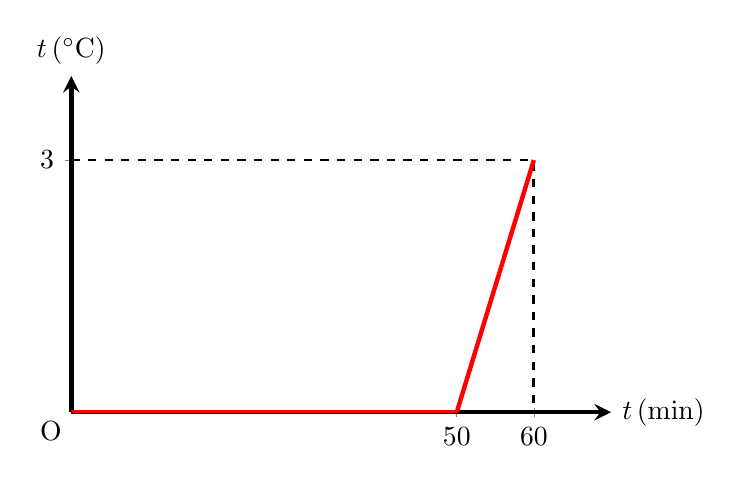
\begin{tikzpicture}  
			\begin{axis}[  ultra thick,yscale=0.75,
				xmin=0,  
				xmax=70,  
				xtick={0,50,60},
				ytick={0,3},
				ymin=0,  
				ymax=4, 
				samples=300,
				axis lines=center, 
				xlabel=$\xsi{t}{\left(\si{\minute}\right)}$, 		ylabel=$\xsi{t}{\left(\si{\celsius}\right)}$,
				every axis y label/.style={at=(current axis.above origin),anchor=south},  
				every axis x label/.style={at=(current axis.right of origin),anchor=west},  ]
				\draw[dashed, line width=1pt] (axis cs: 0,3)--++(axis cs: 60,0)--++(axis cs: 0,-3);
				\addplot [ultra thick, red, smooth, domain=0:50] {0};  
				\addplot [ultra thick, red, smooth, domain=50:60] {0.3*(x-50)} ;
				\coordinate (O) at (axis cs: 0,0) ;
				
			\end{axis}  
			\node[below left] at(O){O};
		\end{tikzpicture}
	\end{center}
	\choice
	{$\SI{5.54}{\kilogram}$}
	{\True $\SI{0.63}{\kilogram}$}
	{$\SI{0.54}{\kilogram}$}
	{$\SI{1.26}{\kilogram}$}
	\loigiai{
	Nhiệt lượng phòng tỏa ra trong khoảng thời gian từ $\SI{50}{\minute}$ đến $\SI{60}{\minute}$:
	$$Q=Mc\Delta t=\left(\SI{6.8}{\kilogram}\right)\cdot\left(\SI{4200}{\joule/\kilogram\cdot\kelvin}\right)\cdot\left(\SI{3}{\kelvin}\right)=\SI{85680}{\joule}$$
	Khối lượng nước đá trong hỗn hợp:
	$$m_{\text{đ}}=\dfrac{5Q}{\lambda}=\SI{1.26}{\kilogram}.$$
	Khối lượng nước đá còn lại ở thời điểm phút thứ 25:
	$$m'=\dfrac{m_{\text{đ}}}{2}=\SI{0.63}{\kilogram}.$$
	}
\end{ex}
% ===================================================================
\begin{ex}
	Có hai bình cách nhiệt: bình 1 chứa $\SI{2}{\kilogram}$ nước ở $\SI{20}{\celsius}$, bình 2 chứa $\SI{5}{\kilogram}$ nước ở $\SI{60}{\celsius}$. Ban đầu, người ta rót $\xsi{\Delta m}{\left(\kilogram\right)}$ nước từ bình 1 sang bình 2. Khi bình 2 cân bằng nhiệt, người ta lại rót $2\xsi{\Delta m}{\left(\kilogram\right)}$ nước từ bình 2 về bình 1. Khi bình 1 cân bằng nhiệt thì độ chênh lệch nhiệt độ giữa hai bình lúc này là $\SI{20}{\celsius}$. Giá trị của $\Delta m$ là
	\choice
	{$\SI{0.65}{\kilogram}$}
	{$\SI{0.45}{\kilogram}$}
	{\True $\SI{0.57}{\kilogram}$}
	{$\SI{0.35}{\kilogram}$}
	\loigiai{
	\textbf{* Khi rót $\Delta m$ từ bình 1 sang bình 2:}\\
	$$m_2c\left(t_{\text{cb2}}-t_2\right)+c\left(t_{\text{cb2}}-t_1\right)\Delta m=0\Rightarrow t_{\text{cb2}}=\dfrac{m_2t_2+t_1\Delta m}{m_2+\Delta m}=\dfrac{300+20\Delta m}{5+\Delta m}.$$
	\textbf{* Khi rót $2\Delta m$ từ bình 2 sang bình 1:}\\
	$$\left(m_1-\Delta m\right)c\left(t_{\text{cb1}}-t_1\right)+c\left(t_{\text{cb1}}-t_{\text{cb2}}\right)\cdot2\Delta m=0\Rightarrow t_{\text{cb1}}=\dfrac{2\left(t_{\text{cb2}}-t_{\text{cb1}}\right)\Delta m}{2-\Delta m}+20=\dfrac{40\Delta m}{2-\Delta m}+20$$
	Mà $t_{\text{cb2}}-t_{\text{cb1}}=20\Rightarrow \Delta m\approx\SI{0.57}{\kilogram}.$
	}
\end{ex}
\Closesolutionfile{ans}
\section{Câu trắc nghiệm đúng sai}
\textit{Thí sinh trả lời từ câu 1 đến câu 4. Trong mỗi ý \textbf{a)}, \textbf{b}, \textbf{c)}, \textbf{d)} ở mỗi câu, thí sinh chọn đúng hoặc sai}
\setcounter{ex}{0}
\Opensolutionfile{ans}[ans/Y24-VN12-PH-C1-TF]
% ===================================================================
\begin{ex}
	Xét cấu trúc của chất lỏng thì
	\choiceTF[t]
	{\True khoảng cách trung bình giữa các phân tử trong chất lỏng lớn hơn khoảng cách trung bình giữa các phân tử trong chất rắn và nhỏ hơn khoảng cách trung bình của các phân tử trong chất khí}
	{các phân tử chất lỏng dao động xung quanh vị trí cân bằng cố định}
	{\True chất lỏng có thể tích xác định nhưng không có hình dạng xác định mà hình dạng của nó phụ thuộc vào hình dạng của phần bình chứa nó}
	{\True lực tương tác giữa các phân tử ở thể lỏng lớn hơn lực tương tác giữa các phân tử ở thể khí}
	\loigiai{}
\end{ex}
% ===================================================================
\begin{ex}
	\immini{
		Máy thuỷ lực là một thiết bị quan trọng trong ngành xây dựng, kỹ thuật ô tô, \dots. Bên trong máy thuỷ lực người ta dùng một chất lỏng (dầu thuỷ lực). Khi ta tác dụng một lực $f$ lên piston nhỏ có diện tích $s$ lực này gây ra áp suất $p=f/s$ và được truyền nguyên vẹn đến piston lớn có diện tích $S$ và gây ra lực nâng $F$.	
	}
	{
		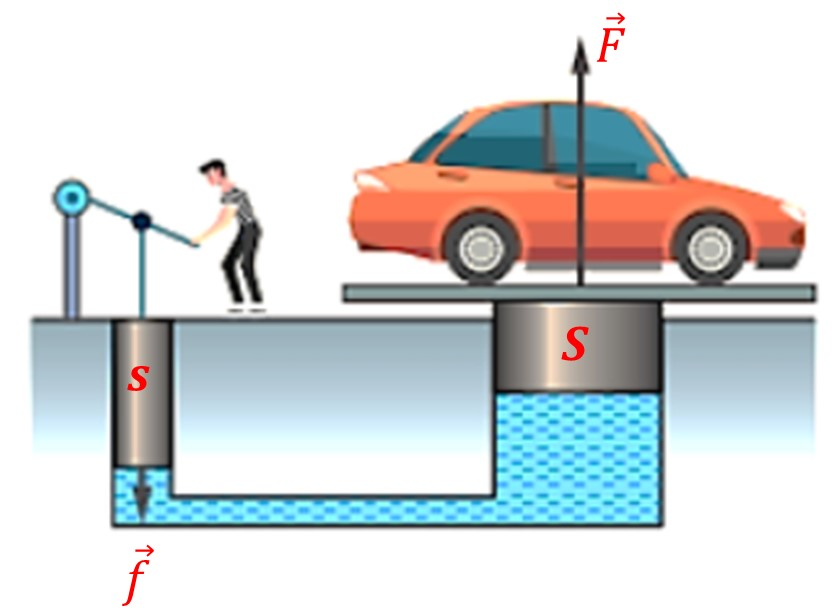
\includegraphics[width=0.6\linewidth]{../figs/Y24-VN12-PH-C1-BT-1}
	}
	\choiceTF[t]
	{Có thể thay thế chất lỏng trong máy thuỷ lực bằng chất khí}
	{Người ta sử dụng dầu thuỷ lực vì dầu thuỷ lực có đặc tính rất khó bị nén}
	{\True Nếu người ta nén với lực $f$ rất lón, các phân tử chất lỏng trong máy thuỷ lực càng bị nén chặt và có thể chuyển sang thể rắn}
	{Giả sử piston lớn có diện tích gấp 50 lần piston nhỏ. Khi đó, nếu muốn nâng một xe có khối lượng $\SI{1500}{\kilogram}$ thì cần tác dụng lên piston nhỏ một lực $\SI{30}{\newton}$}
	\loigiai{
		\begin{itemchoice}
			\itemch Sai. Vì chất khí dễ bị nén nên máy không hoạt động được.
			\itemch Đúng.
			\itemch Sai. Chất lỏng không thể chuyển thành thể rắn khi chỉ bị nén.
			\itemch Sai. $p=\dfrac{f}{s}=\dfrac{F}{S}\Rightarrow f=\dfrac{Fs}{S}=\SI{300}{\newton}$.
			
		\end{itemchoice}	
	}
\end{ex}
% ===================================================================
\begin{ex}
	Một khối băng có khối lượng $m =\SI{800}{\gram}$ ở $\SI{-10}{\celsius}$. Biết nhiệt dung riêng của nước đá là $c_{\text{đ}}= \SI{2090}{\joule/\kilogram\cdot\kelvin}$; nhiệt dung riêng của nước là $c_n =\SI{4190}{\joule/\kilogram\cdot\kelvin}$ và nhiệt nóng chảy riêng của nước đá $\lambda=\SI{3.33E5}{\joule/\kilogram}$.
	\choiceTF[t]
	{Để nóng chảy hoàn toàn, khối băng cần nhận được một năng lượng xấp xỉ $\SI{16720}{\joule}$}
	{Khi ở  $\SI{0}{\celsius}$, nếu truyền một nhiệt lượng $\SI{3352}{\joule}$ thì khối băng tan hoàn toàn thành nước ở nhiệt độ $\SI{0}{\celsius}$}
	{\True Khi băng bắt đầu nóng chảy, nếu nhận được nhiệt lượng $\SI{83.25}{\kilo\joule}$ thì khối lượng băng còn lại là $\SI{550}{\gram}$}
	{\True Cần một năng lượng $\SI{336.92}{\kilo\joule}$ truyền cho khối băng để nó chuyển hoàn toàn sang trạng thái lỏng ở $\SI{25}{\celsius}$}
	\loigiai{
	\begin{itemchoice}
		\itemch Sai. $Q=mc_{\text{đ}}\Delta t+m\lambda=\SI{283120}{\joule}$.
		\itemch Sai. $Q=m\lambda=\SI{266400}{\joule}$.
		\itemch Đúng.
		\itemch Đúng.
	\end{itemchoice}
	}
\end{ex}
% ===================================================================
\begin{ex}
	Người ta dùng một lò hồ quang điện để nấu chảy một khối kim loại nặng $\SI{29}{\kilogram}$. Biết mỗi phút lò hồ quang cung cấp cho khối kim loại một nhiệt lượng không đổi là $\SI{400}{\kilo\joule}$. Sự thay đổi nhiệt độ của khối kim loại được ghi lại theo thời gian như hình vẽ.
	\begin{center}
		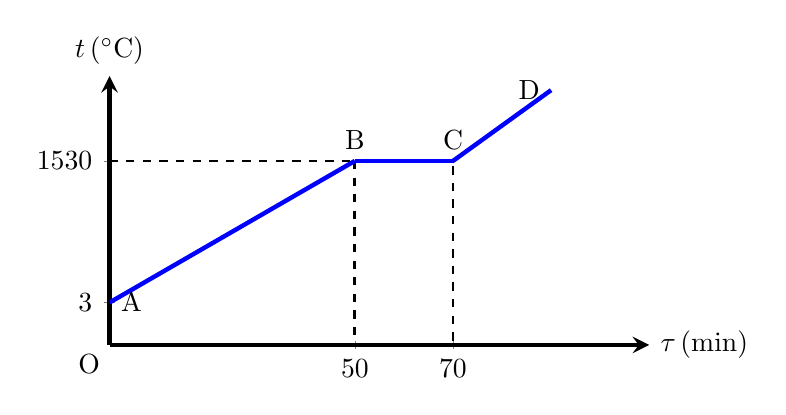
\begin{tikzpicture}  
			\begin{axis}[  ultra thick,yscale=0.6,
				xmin=0,  
				xmax=110,  
				xtick={0,50,70},
				ytick={0,3,13},
				yticklabels={0,3,1530},
				ymin=0,  
				ymax=19, 
				samples=300,
				axis lines=center, 
				xlabel=$\xsi{\tau}{\left(\si{\minute}\right)}$, 		ylabel=$\xsi{t}{\left(\si{\celsius}\right)}$,
				every axis y label/.style={at=(current axis.above origin),anchor=south},  
				every axis x label/.style={at=(current axis.right of origin),anchor=west},  ]
				\draw[dashed, line width=1pt] (axis cs: 0,13)--++(axis cs: 70,0)--++(axis cs: 0,-13);
				\draw[dashed, line width=1pt] (axis cs: 50,13)--(axis cs: 50,0);
				\addplot [ultra thick, blue, smooth, domain=0:50] {3+0.2*x};  
				\addplot [ultra thick, blue, smooth, domain=50:70] {13};
				\addplot [ultra thick, blue, smooth, domain=70:90] {13+0.25*(x-70)};
				\node[right] at (0,3) {A};
				\node[above] at (50,13) {B};
				\node[above] at (70,13) {C};
				\node[left] at (90,18) {D};
				\coordinate (O) at (axis cs: 0,0);
			\end{axis}  
			\node[below left] at (O) {O};
		\end{tikzpicture}
	\end{center}
	\choiceTF[t]
	{Giai đoạn AB trên đồ thị tương ứng với quá trình nóng chảy của kim loại}
	{Giai đoạn BC khối kim loại không nhận thêm nhiệt lượng từ lò nung}
	{\True Nhiệt dung riêng của khối kim loại xấp xỉ $\SI{459.8}{\joule/\kilogram\cdot\kelvin}$}
	{\True Nhiệt nóng chảy riêng của khối kim loại xấp xỉ $\SI{276E3}{\joule/\kilogram}$}
	\loigiai{
	\begin{itemchoice}
		\itemch Sai. Giai đoạn AB khối kim loại được nung nóng và đang tăng nhiệt độ.
		\itemch Sai. Khối kim loại vẫn nhận thêm nhiệt lượng và đang nóng chảy.
		\itemch Đúng.
		\itemch Đúng.
	\end{itemchoice}
	}
\end{ex}
\Closesolutionfile{ans}
\section{Câu trắc nghiệm trả lời ngắn} \textit{Thí sinh trả lời từ câu 1 đến câu 6}
\setcounter{ex}{0}
\Opensolutionfile{ans}[ans/Y24-VN12-PH-C1-TL]
% ===============================================================
\begin{ex}
Những viên nước đá ở $\SI{0}{\celsius}$ và khối lượng mỗi viên là $\SI{200}{\gram}$ lần lượt được thả vào $\SI{2}{\kilogram}$ nước ở $\SI{32}{\celsius}$ sao cho khi viên nước đá trước khi tan hết thì viên tiếp theo mới được thả vào. Cho biết năng lượng nhiệt cần thiết để làm tan $\SI{1}{\gram}$ nước đá  là $\SI{334}{\joule}$ và nhiệt dung riêng của nước là $\SI{4.18}{\joule/\left(\gram\cdot\kelvin\right)}$. Xác định số viên đá tối đa có thể thả vào lượng nước trên để trong nước không còn sót lại phần đá nào.	
	\shortans{4}
	\loigiai{
		Nhiệt lượng nước tỏa ra để giảm từ $\SI{32}{\celsius}$ xuống còn $\SI{0}{\celsius}$ có thể làm tan tối đa số viên đá là:
		$$N=\dfrac{m_nct_0}{\lambda m_\text{đ}}=4,005.$$
	}
\end{ex}
% ===============================================================
\begin{ex}
Biết rằng khoảng cách mỗi độ chia trong thang đo nhiệt độ X tương ứng với 1,5 độ chia trong thang đo nhiệt độ Y. Một vật khi có nhiệt độ $\SI{25}{\degree X}$ sẽ có nhiệt độ tương ứng là $\SI{45}{\degree Y}$ trong thang đo nhiệt độ Y. Khi nhiệt độ đo được ở thang Y là $\SI{50}{\degree Y}$ thì nhiệt độ tương ứng trong thang X là bao nhiêu $\si{\degree X}$?	
	\shortans{32,5 }
	\loigiai{
		$$\left(T_X-\SI{25}{\degree X}\right)\cdot1=\left(T_Y-\SI{45}{\degree Y}\right)\cdot 1,5\Rightarrow T_X=1,5T_Y-42,5$$
		Khi $T_Y=\SI{50}{\degree Y}$ thì $T_X=\SI{32.5}{\degree X}$.
	}
\end{ex}
% ===============================================================
\begin{ex}
Một khối khí được đặt trong một xilanh nằm ngang, được đậy kín bằng một pit-tông. Người ta cung cấp cho khối khí một nhiệt lượng $\SI{5}{\joule}$. Lúc này khối khí nở ra và đẩy pit-tông dịch chuyển (coi là chuyển động đều) một đoạn $\SI{10}{\centi\meter}$. Biết rằng lực ma sát giữa pit-tông và xilanh có độ lớn $F_{\text{ms}} =\SI{10}{\newton}$. Tính độ biến thiên nội năng của khối khí theo đơn vị $\si{\joule}$.	
	\shortans{4}
	\loigiai{
	Công do khối khí thực hiện:
	$$A'=Fs=\left(\SI{10}{\newton}\right)\cdot\left(\SI{0.1}{\meter}\right)=\SI{1}{\joule}.$$
	Độ biến thiên nội năng của khối khí:
	$$\Delta U=Q+A=Q-A'=\SI{4}{\joule}.$$	
	}
\end{ex}
% ===============================================================
\begin{ex}
	Một người cọ xát một miếng sắt dẹt có khối lượng $\SI{150}{\gram}$ trên một tấm đá mài. Sau một khoảng thời gian, miếng sắt nóng thêm $\SI{12}{\celsius}$. Giả sử rằng $\SI{40}{\percent}$ công đó được dùng để làm nóng miếng sắt. Biết nhiệt dung riêng của sắt là $\SI{460}{\joule/\kilogram\cdot\kelvin}$. Công mà người này đã thực hiện là bao nhiêu $\si{\joule}$?
	\shortans{2070 }
	\loigiai{
		$A=\dfrac{mc\Delta t}{H}=\SI{2070}{\joule}.$
	}
\end{ex}
% ===============================================================
\begin{ex}
Trong thí nghiệm đo nhiệt dung riêng của nước, công suất điện trên oát kế là $\SI{950}{\watt}$, khối lượng nước được sử dụng là $\SI{1}{\kilogram}$. Đồ thị thực nghiệm nhiệt độ phụ thuộc vào thời gian xác định được như hình bên dưới.
\begin{center}
	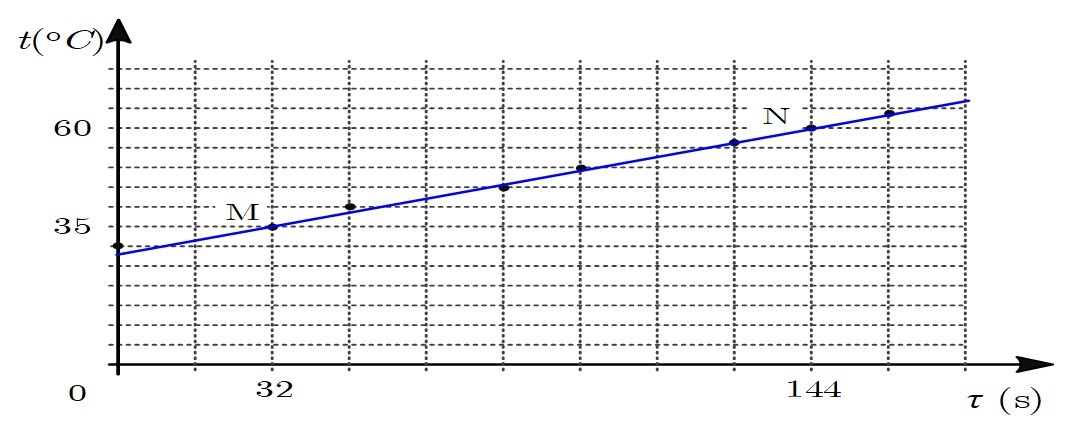
\includegraphics[width=0.7\linewidth]{../figs/Y24-VN12-PH-C1-BT-2}
\end{center}	
Hãy tính nhiệt dung riêng của nước ra đơn vị J/kg.K.
	\shortans{ 4256}
	\loigiai{
		$$c=\dfrac{\calP t}{m\Delta t}=\dfrac{\left(\SI{950}{\watt}\right)\cdot\left(\SI{144}{\second}-\SI{32}{\second}\right)}{\left(\SI{1}{\kilogram}\right)\cdot\left(\SI{60}{\celsius}-\SI{35}{\celsius}\right)}=\SI{4256}{\joule/\kilogram\cdot\kelvin}.$$
	}
\end{ex}
% ===============================================================
\begin{ex}
Có ba bình nước giống nhau, mỗi bình chứa $\SI{20}{\gram}$ nước ở cùng nhiệt độ. Người ta thả vào mỗi bình một cục nước đá có khối lượng khác nhau nhưng có cùng nhiệt độ. Bình 1 được thả cục nước đá có khối lượng $\SI{10}{\gram}$, khi cân bằng nhiệt, khối lượng nước đá còn lại trong bình là $\SI{9}{\gram}$. Bình 2 được thả cục nước đá có khối lượng $\SI{20}{\gram}$, khi cân bằng nhiệt, khối lượng nước đá trong bình không đổi. Bình 3 được thả cục nước đá có khối lượng $\SI{40}{\gram}$, khi có cân bằng nhiệt, khối lượng nước đá trong bình là bao nhiêu gram?	
	\shortans{42 }
	\loigiai{
		Bình 1 chỉ có $\Delta m_1=\SI{1}{\gram}$ đá tan thành nước $\Rightarrow$ nhiệt độ cân bằng của hỗn hợp là $\SI{0}{\celsius}$:
		$$m_nc_nt_n=m_{\text{đ1}}c\left(0-t_{\text{đ}}\right)+\lambda\Delta m_1$$
		\begin{equation}
			\Rightarrow 20c_nt_n=-10ct_{\text{đ}}+\lambda
			\label{eq: 1}
		\end{equation}
		Bình 2 có khối lượng nước đá không đổi, chứng tỏ nhiệt lượng nước tỏa ra để giảm nhiệt độ xuống $\SI{0}{\celsius}$ bằng nhiệt lượng nước đá thu vào để tăng nhiệt độ lên $\SI{0}{\celsius}$.
		\begin{equation}
			m_nc_nt_n=-m_{\text{đ2}}ct_{\text{đ}}
			\Leftrightarrow c_nt_n=-c_\text{đ}t_{\text{đ}}
			\label{eq: 2}
		\end{equation}
		Từ \eqref{eq: 1} và \eqref{eq: 2}, suy ra:
		$$\begin{cases}
		c_nt_n=0,1\lambda\\
			ct_{\text{đ}}=-0,1\lambda
		\end{cases}$$
		Bình 3 được thả cục nước đá có khối lượng $\SI{40}{\gram}$ nên nước sẽ bị đóng băng, khối lượng nước đóng băng là $m_{\text{b}}$:
		$$m_nc_nt_n+m_b\lambda=-m_{\text{đ3}}ct_{\text{đ}}\Leftrightarrow 20\cdot0,1\lambda+m_b\lambda=40\cdot0,1\lambda\Rightarrow m_{\text{b}}=\SI{2}{\gram}.$$
		Vậy bình 3 khi cân bằng nhiệt thì khối lượng nước đá là $m_{\text{đ3}}+m_{\text{b}}=\SI{42}{\gram}.$
	}
\end{ex}
\Closesolutionfile{ans}


%	\stopcontents[mychapters]
%		\mychapter{KHÍ LÍ TƯỞNG}
%	\startcontents[mychapters]
%	\printcontents[mychapters]{}{0}{\setcounter{tocdepth}{1}}
%	\begin{center}
%		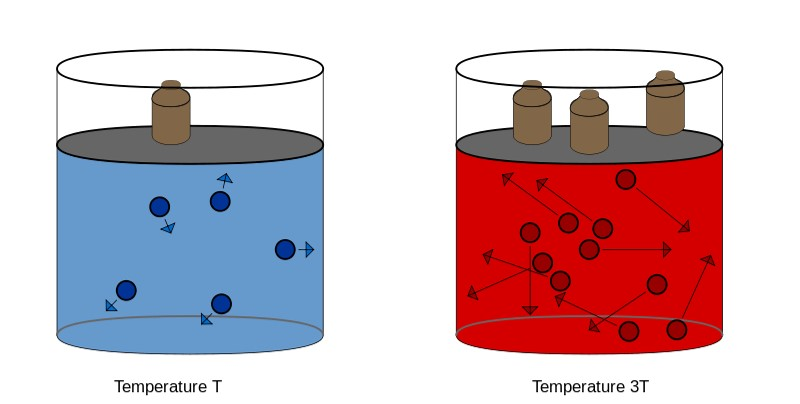
\includegraphics[width=0.7\linewidth]{../figs/G12C2}
%	\end{center}
%	\chapter{Tóm tắt lý thuyết}
\section{Mô hình động học phân tử chất khí}
\subsection{Chuyển động Brown}
\begin{itemize}
	\item Chuyển động Brown là chuyển động hỗn loạn, không ngừng, không theo quy luật, có quỹ đạo là đường gấp khúc bất kì của các hạt nhẹ trong chất lỏng và chất khí.
	\item Chuyển động Brown chứng tỏ các phân tử khí chuyển động hỗn loạn, không ngừng.
	\item Nhiệt độ càng cao, các phân tử khí chuyển động càng nhanh.
\end{itemize}
\subsection{Thuyết động học phân tử chất khí}
\begin{itemize}
	\item Chất khí được cấu tạo từ các phân tử có kích thước rất nhỏ so với khoảng cách trung bình giữa chúng.
	\item Các phân tử khí luôn chuyển động hỗn loạn, không ngừng. Nhiệt độ càng cao, các phân tử khí chuyển động càng nhanh.
	\item Trong quá trình chuyển động, các phân tử khí va chạm với thành bình chứa, gây ra áp suất lên thành bình.
\end{itemize}
\subsection{Lượng chất}
\begin{itemize}
	\item Đơn vị đo lượng chất là $\si{\mole}$.
	\item Mol là lượng chất trong đó chứa số phân tử (hoặc nguyên tử) bằng $N_A = \SI{6.022E23}{\mole^{-1}}$.	$N_A$ được gọi là số Avogadro.
	\item Một mẫu chất có khối lượng $m$, chứa $N$ phân tử thì có số mol là: $n=\dfrac{N}{N_A}=\dfrac{m}{M}$, trong đó
	$M$ (khối lượng mol) là khối lượng của 1 mol chất đó.
\end{itemize}
\section{Phương trình trạng thái khí lí tưởng}
\subsection{Định luật Boyle}
\begin{itemize}
	\item Ở nhiệt độ không đổi, áp suất của một khối lượng khí xác định tỉ lệ nghịch với thể tích	của nó.
	$$pV=\text{hằng số}\quad \text{hay}\quad p_1V_1=p_2$$
	\item Đồ thị biểu diễn sự phụ thuộc của áp suất theo thể tích khi nhiệt độ của khối khí không đổi được gọi là đường đẳng nhiệt.
	\begin{center}
		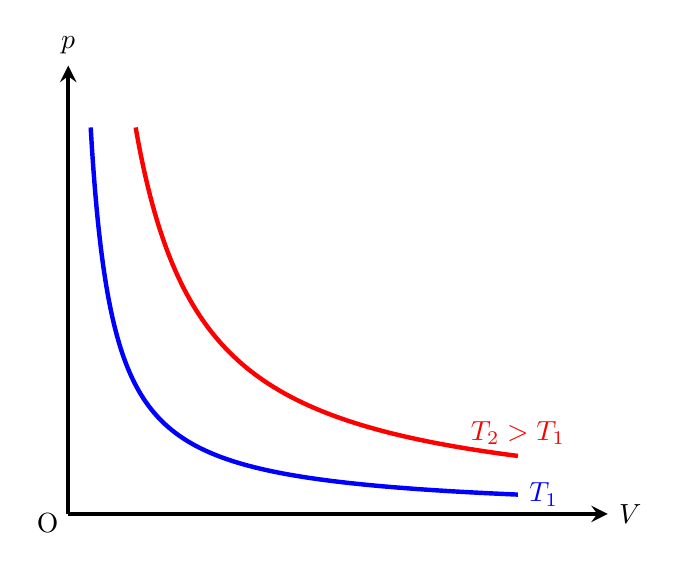
\begin{tikzpicture}  
			\begin{axis}[  ultra thick,
				xmin=0,  
				xmax=24,  
				xtick=\empty,
				ytick=\empty,
				ymin=0,  
				ymax=5.8, 
				samples=300,
				xticklabels=\empty,
				yticklabels=\empty,
				axis lines=center, 
				xlabel=$V$, 
				ylabel=$p$, 
				every axis y label/.style={at=(current axis.above origin),anchor=south},  
				every axis x label/.style={at=(current axis.right of origin),anchor=west},  ]
				\addplot [ultra thick, blue, smooth, domain=1:20] {5/x} node[right] {$T_1$}; 
				\addplot [ultra thick, red, smooth, domain=3:20] {15/x} node[above] {$T_2>T_1$}; 
			\end{axis}  
			\node[label={[below left]90:O}] at (0,0){};
		\end{tikzpicture}
	\end{center}
\end{itemize}
\subsection{Định luật Charles}
\begin{itemize}
	\item Ở áp suất không đổi, thể tích của một khối lượng khí xác định tỉ lệ thuận với nhiệt độ tuyệt đối của nó.
	$$\dfrac{V}{T}=\text{hằng số}\quad \text{hay}\quad \dfrac{V_1}{T_1}=\dfrac{V_2}{T_2}$$
	\item Đồ thị biểu diễn sự phụ thuộc của thể tích theo nhiệt độ tuyệt đối khi áp suất của khối khí không đổi được gọi là đường đẳng áp.
	\begin{center}
		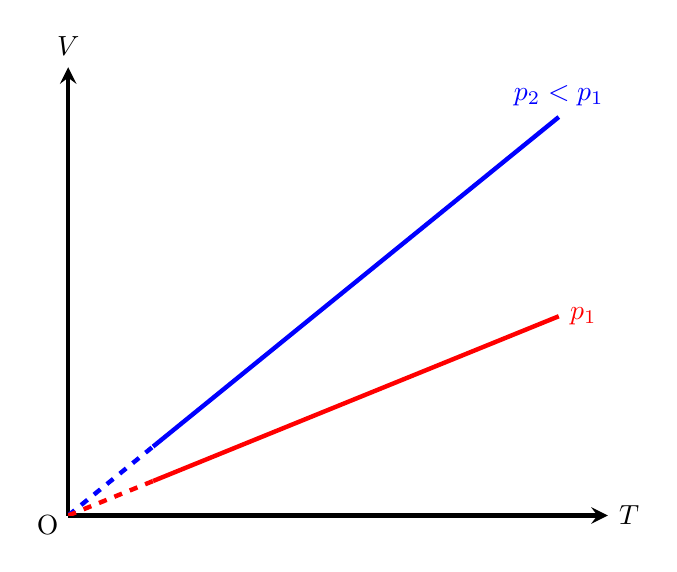
\begin{tikzpicture}  
			\begin{axis}[  ultra thick,
				xmin=0,  
				xmax=1100,  
				xtick=\empty,
				ytick=\empty,
				ymin=0,  
				ymax=900, 
				samples=300,
				xticklabels=\empty,
				yticklabels=\empty,
				axis lines=center, 
				xlabel=$T$, 
				ylabel=$V$, 
				every axis y label/.style={at=(current axis.above origin),anchor=south},  
				every axis x label/.style={at=(current axis.right of origin),anchor=west},  ]
				\addplot [ultra thick, blue, smooth,dashed, domain=0:173] {0.8*x}; 
				\addplot [ultra thick, blue, smooth, domain=173:1000] {0.8*x} node[above]{$p_2<p_1$}; 
				\addplot [ultra thick, red, smooth,dashed, domain=0:173] {0.4*x}; 
				\addplot [ultra thick, red, smooth, domain=173:1000] {0.4*x} node[right]{$p_1$};
			\end{axis}  
			\node[label={[below left]90:O}] at (0,0){};
		\end{tikzpicture}
	\end{center}
\end{itemize}
\subsection{Khí lí tưởng}
\begin{itemize}
	\item Khí lí tưởng là chất khí tuân theo đúng định luật Boyle và định luật Charles.
	\item Nội năng của khí lí tưởng chỉ phụ thuộc vào nhiệt độ.
\end{itemize}
\subsection{Phương trình trạng thái của khí lí tưởng}
$$\dfrac{pV}{T}=nR\quad \text{hay}\quad \dfrac{p_1V_1}{T_1}=\dfrac{p_2V_2}{T_2}$$
Trong đó, $R\approx \SI{8.31}{\joule/\mole\cdot\kelvin} \approx\SI{0.082}{\dfrac{\liter\cdot atm}{\mole\cdot\kelvin}}$
là hằng số khí lí tưởng; $n$ là số mol khí.
%	\chapter{Câu hỏi ôn tập}
\hideall{
\setcounter{section}{0}
\begin{center}
	\textbf{\large BẢNG ĐÁP ÁN}
\end{center}
\section{Câu trắc nghiệm nhiều phương án lựa chọn}
\inputansbox{10}{ans/Y24-VN12-PH-C2-TN}
\section{Câu trắc nghiệm đúng sai}
\inputansbox[2]{2}{ans/Y24-VN12-PH-C2-TF}
\section{Câu trắc nghiệm trả lời ngắn}
\inputansbox[3]{6}{ans/Y24-VN12-PH-C2-TL}
}
\setcounter{section}{0}
\section{Câu trắc nghiệm nhiều phương án lựa chọn}
\textit{Thí sinh trả lời từ câu 1 đến câu 18. Mỗi câu thí sinh chọn một phương án}
\setcounter{ex}{0}
\Opensolutionfile{ans}[ans/Y24-VN12-PH-C2-TN]
% ===================================================================
\begin{ex}
	heo thuyết động học phân tử chất khí, áp suất của một khối lượng khí nhất định chứa trong một bình có thể tích xác định giảm là vì
	\begin{enumerate}[label=(\arabic*)]
		\item tốc độ trung bình của các phân tử khí giảm.
		\item các phân tử khí va chạm với thành bình chứa ít thường xuyên hơn.
		\item nhiệt độ của chất khí giảm.
	\end{enumerate}
	Nhận định nào đúng?
	\choice
	{Chỉ (2)}
	{(1) và (2)}
	{(1) và (3)}
	{\True (1), (2) và (3)}
	\loigiai{}
\end{ex}
% ===================================================================
\begin{ex}
	Khi một chất khí trong một bình kín bị đun nóng, áp suất chất khí tăng lên. Phát biểu nào sau đây giải thích đúng hiện tượng này?
	\choice
	{Các phân tử khí dãn nở và trở nên nặng hơn, vì thế chúng va chạm nhau mạnh hơn}
	{Các phân tử khí có ít không gian chuyển động hơn, nên chúng va chạm nhau thường xuyên hơn}
	{Các phân tử khí va chạm vào thành bình mạnh hơn nhưng ít thường xuyên hơn}
	{\True Các phân tử khí chuyển động nhanh hơn, vì thế chúng va chạm với thành bình thường xuyên hơn}
	\loigiai{}
\end{ex}
% ===================================================================
\begin{ex}
	Một khối khí nhất định được chứa trong một xilanh kín với một pit-tông động. Ban đầu, khối khí ở áp suất $p_1$ và có thể tích $V_1$. Nhiệt độ được giữ không đổi. Pit-tông dịch chuyển sao cho áp suất trở thành $p_2$ và thể tích trở thành $V_2$. Chỉ ra biểu thức đúng.
	\choice
	{$\dfrac{p_1}{V_1}=\dfrac{p_2}{V_2}$}
	{$\dfrac{p_1}{p_2}=\dfrac{V_1}{V_2}$}
	{\True $p_1 V_1=p_2 V_2$}
	{$p_1 V_2=p_2 V_1$}
	\loigiai{}
\end{ex}
% ===================================================================
\begin{ex}
	Trong hệ tọa độ $(p, V)$, đường biểu diễn quá trình đẳng nhiệt của một khối khí lí tưởng có dạng
	\choice
	{một đường thẳng đứng}
	{một phần của elip}
	{một phần của parabol}
	{\True một phần của hyperbol}
	\loigiai{}
\end{ex}
% ===================================================================
\begin{ex}
	\immini{
	Hình bên mô tả một khối khí bị giữ bên trong một xilanh bởi một pit-tông động. Thể tích của khối khí là $\SI{120}{\centi\meter^3}$ và áp suất của khối khí là $p$. Từ từ di chuyển pit-tông sang trái sao cho thể tích khối khí giảm còn $\SI{30}{\centi\meter^3}$. Nhiệt độ của khối khí không đổi. Áp suất mới của khối khí trong xilanh là bao nhiêu?
	}
	{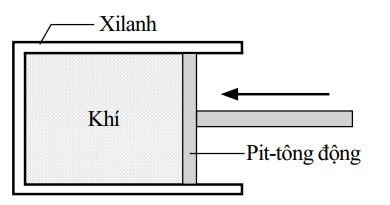
\includegraphics[width=0.5\linewidth]{../figs/G12C2-1}}
	\choice
	{$\dfrac{p}{4}$}
	{$\dfrac{p}{2}$}
	{$p$}
	{\True $4 p$}
	\loigiai{}
\end{ex}
% ===================================================================
\begin{ex}
	Có $\SI{400}{\centi\meter^3}$ khí lí tưởng ở $\SI{0}{\celsius}$. Nếu được đun nóng ở áp suất không đổi để nhiệt độ tăng lên đến $\SI{10}{\celsius}$ thì khối khí sẽ chiếm thể tích
	\choice
	{\True $\SI{415}{\centi\meter^3}$}
	{$\SI{283}{\centi\meter^3}$}
	{$\SI{278}{\centi\meter^3}$}
	{$\SI{493}{\centi\meter^3}$}
	\loigiai{}
\end{ex}
% ===================================================================
\begin{ex}
	Hai bình có thể tích bằng nhau chứa cùng một loại khí. Áp suất và nhiệt độ tuyệt đối của khí trong mỗi bình lần lượt là $p_1$ và $p_2, T_1$ và $T_2$. Hai bình được nối thông với nhau và chất khí đạt tới áp suất chung $p$ và nhiệt độ tuyệt đối chung $T$. Chỉ ra biểu thức đúng.
	\choice
	{$\dfrac{p}{T}=\dfrac{p_1}{T_1}+\dfrac{p_2}{T_2}$}
	{\True $\dfrac{p}{T}=\dfrac{1}{2}\left(\dfrac{p_1}{T_1}+\dfrac{p_2}{T_2}\right)$}
	{$\dfrac{p}{T}=\dfrac{p_1 T_2+p_2 T_1}{2\left(T_1+T_2\right)}$}
	{$\dfrac{p}{T}=\dfrac{p_1+p_2}{T_1+T_2}$}
	\loigiai{}
\end{ex}
% ===================================================================
\begin{ex}
	Giả sử một khối khí ban đầu ở nhiệt độ chuẩn và khối khí chịu sự biến đổi sao cho áp suất của nó tăng gấp bốn lần còn nhiệt độ tuyệt đối của nó giảm đi một nửa. Thể tích của khối khí biến đổi như thế nào trong quá trình này?
	\choice
	{Tăng 8 lần}
	{\True Giảm 8 lần}
	{Không đổi}
	{Tăng 2 lần}
	\loigiai{}
\end{ex}
% ===================================================================
\begin{ex}
	\immini{
	Một khối khí thực hiện các quá trình biến đổi trạng thái như hình bên. Chỉ ra đáp án \textbf{sai}.
	\choice
	{CA là quá trình dãn nở đẳng nhiệt}
	{$p_{\mathrm{A}} V_{\mathrm{A}}=p_{\mathrm{C}} V_{\mathrm{C}}$}
	{\True AB là quá trình nén đẳng tích}
	{$\dfrac{V_{\mathrm{A}}}{T_{\mathrm{A}}}=\dfrac{V_{\mathrm{B}}}{T_{\mathrm{B}}}$}
	}
	{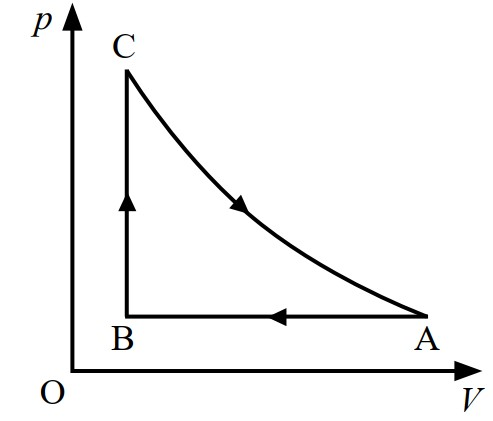
\includegraphics[width=0.5\linewidth]{../figs/G12C2-2}}
	\loigiai{}
\end{ex}
% ===================================================================
\begin{ex}
	 \immini{
	 Một khối khí thực hiện quá trình biến đổi từ trạng thái (1) sang trạng thái (2) như hình bên. Hình nào sau đây biểu diễn đúng quá trình biến đổi của khối khí từ trạng thái (1) sang trạng thái (2) trong hệ tọa độ $(T, p)$?
	 }
	 {
	 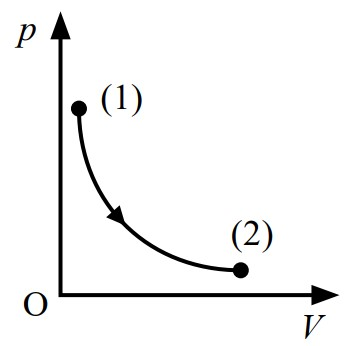
\includegraphics[width=0.4\linewidth]{../figs/G12C2-3}
	 }
	 \begin{center}
	 	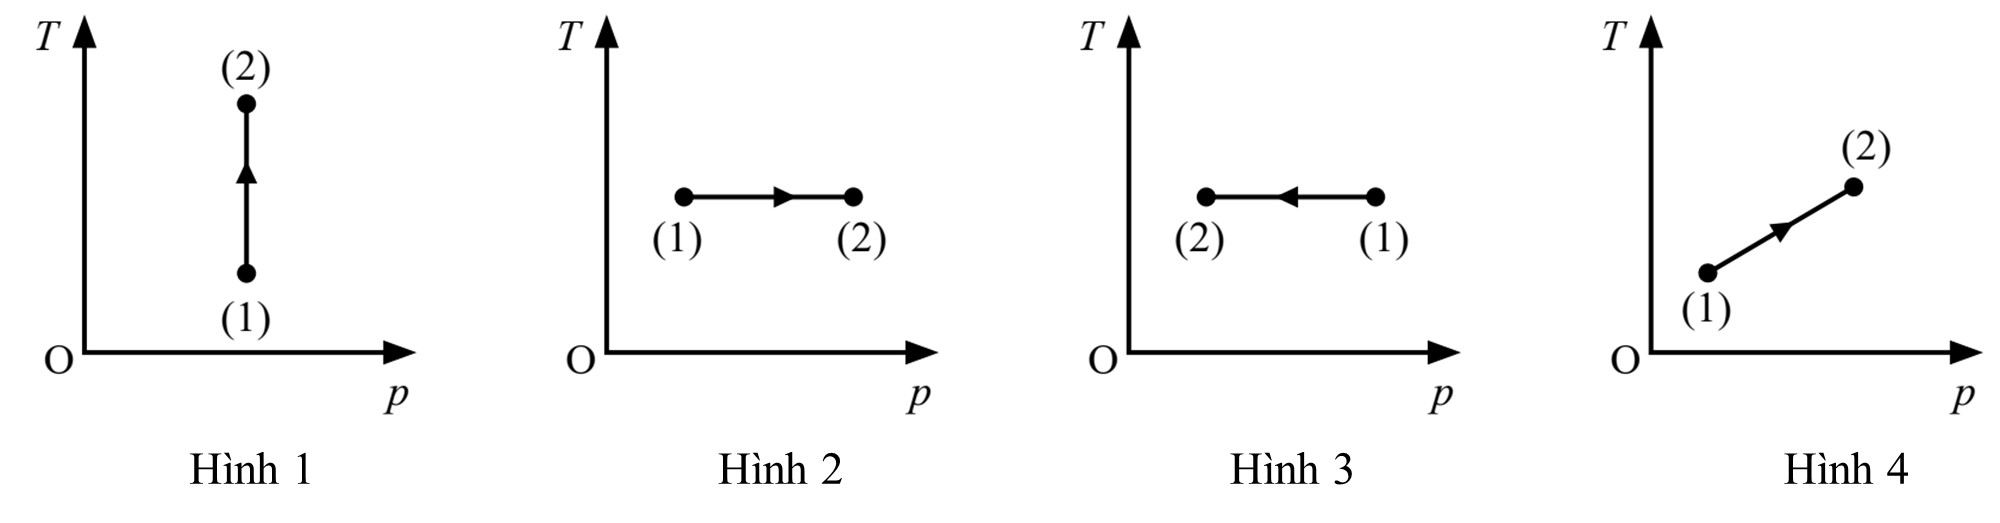
\includegraphics[width=0.8\linewidth]{../figs/G12C2-4}
	 \end{center}
	\choice
	{Hình 1}
	{Hình 2}
	{\True Hình 3}
	{Hình 4}
	\loigiai{}
\end{ex}
% ===================================================================
\begin{ex}
	Một bọt khí tăng gấp đôi bán kính của nó khi nổi từ đáy hồ lên mặt nước. Giả sử bọt khí nổi lên từ từ (nhiệt độ không đổi) và áp suất khí quyển bằng áp suất của một cột nước có độ cao $H$, thì độ sâu của hồ là
	\choice
	{$4 H$}
	{$5 H$}
	{\True $7 H$}
	{$14 H$}
	\loigiai{}
\end{ex}
% ===================================================================
\begin{ex}
	Một quả bóng được bơm đầy khí nitrogen tinh khiết. Quả bóng được xác định có thể tích $\SI{0.75}{\liter}$ vào một ngày có nhiệt độ $\SI{20}{\celsius}$ và áp suất không khí là $\SI{0.85}{atm}$. Có bao nhiêu phân tử nitrogen trong quả bóng?
	\choice
	{\True $1,6 \cdot 10^{22}$}
	{$2,1\cdot10^{20}$}
	{$4,7\cdot10^{23}$}
	{$1,6 \cdot 10^{25}$}
	\loigiai{}
\end{ex}
% ===================================================================
\begin{ex}
	Nén đẳng nhiệt một khối khí lí tưởng xác định làm áp suất khí thay đổi một lượng $\SI{0.5}{atm}$. Biết thể tích và áp suất ban đầu của khối khí là $\SI{5}{\liter}$ và $\SI{2}{atm}$. Thể tích của khối khí lúc sau là
	\choice
	{$\SI{6.25}{\liter}$}
	{\True $\SI{4}{\liter}$}
	{$\SI{6.67}{\liter}$}
	{$\SI{20}{\liter}$}
	\loigiai{\begin{center}
			\begin{tabular}{C{4cm} C{3cm} C{4cm}}
				\colorbox{yellow}{\textcolor{red}{\textbf{Trạng thái 1}}} & $\xrightarrow[]{T_1=T_2}$ & \colorbox{yellow}{\textcolor{red}{\textbf{Trạng thái 2}}}\\
				$p_1=\SI{2}{atm}$ & &$p_2=\SI{2.5}{atm}$\\
				$V_1=\SI{5}{\liter}$ & & $V_2=?$
			\end{tabular}
		\end{center}
		Vì thể tích khí giảm nên áp suất khí tăng.\\
		$$V_2=\dfrac{p_1V_1}{p_2}=\SI{4}{\liter}.$$}
\end{ex}
% ===================================================================
\begin{ex}
	Ở nhiệt độ $\SI{273}{\celsius}$ thể tích của một khối khí lí tưởng là $\SI{10}{\liter}$. Trong điều kiện áp suất không đổi, thể tích của khối khí đó ở nhiệt độ $\SI{546}{\celsius}$ là
	\choice
	{$\SI{20}{\liter}$}
	{\True $\SI{15}{\liter}$}
	{$\SI{12}{\liter}$}
	{$\SI{13.5}{\liter}$}
	\loigiai{\begin{center}
			\begin{tabular}{C{4cm} C{3cm} C{4cm}}
				\colorbox{yellow}{\textcolor{red}{\textbf{Trạng thái 1}}} & $\xrightarrow[]{p_1=p_2}$ & \colorbox{yellow}{\textcolor{red}{\textbf{Trạng thái 2}}}\\
				$V_1=\SI{10}{\liter}$ & &$V_2=?$\\
				$T_1=\SI{546}{\kelvin}$ & & $T_2=\SI{819}{\kelvin}$
			\end{tabular}
		\end{center}
		$$\dfrac{V_1}{T_1}=\dfrac{V_2}{T_2}\Rightarrow V_2=\SI{15}{\liter}.$$}
\end{ex}
% ===================================================================
\begin{ex}
	Một bình chứa khí helium có dung tích $\SI{50}{\liter}$ ở nhiệt độ $\SI{25}{\celsius}$ và áp suất $\SI{20}{atm}$. Người ta muốn dùng khí từ bình này để bơm những quả bóng bay đến dung tích $\SI{2500}{\milli\liter}$ và ở áp suất $\SI{1}{atm}$. Coi nhiệt độ khí là không đổi. Xác định số lượng quả bóng bay có thể bơm được?
	\choice
	{40}
	{120}
	{214}
	{\True 400}
	\loigiai{}
\end{ex}
% ===================================================================
\begin{ex}
	Một khối khí dãn nở đẳng áp có thể tích tăng gấp 1,5 lần thì nhiệt độ của nó tăng thêm $\SI{150}{\celsius}$. Nhiệt độ ban đầu của khối khí là
	\choice
	{$\SI{150}{\celsius}$}
	{$\SI{300}{\celsius}$}
	{$\SI{-123}{\celsius}$}
	{\True $\SI{27}{\celsius}$}
	\loigiai{}
\end{ex}
% ===================================================================
\begin{ex}
	Một khối khí được đựng trong bình kín. Nếu ở $\SI{25}{\celsius}$, áp suất của khí trong bình là $\SI{2}{atm}$ thì ở $\SI{250}{\celsius}$, áp suất của khí là
	\choice
	{$\SI{20}{atm}$}
	{\True $\SI{3.51}{atm}$}
	{$\SI{1.14}{atm}$}
	{$\SI{15.4}{atm}$}
	\loigiai{}
\end{ex}
% ===================================================================
\begin{ex}
	Nén $\SI{10}{\liter}$ khí ở nhiệt độ $\SI{27}{\celsius}$ để cho thể tích của nó chỉ còn $\SI{4}{\liter}$. Trong quá trình nén, nhiệt độ khí tăng $\SI{33}{\celsius}$. So với áp suất ban đầu, áp suất khí lúc sau
	\choice
	{\True tăng 2,775 lần}
	{giảm 2,775 lần}
	{giảm 2,55 lần}
	{tăng 2,55 lần}
	\loigiai{\begin{center}
			\begin{tabular}{C{4cm} C{3cm} C{4cm}}
				\colorbox{yellow}{\textcolor{red}{\textbf{Trạng thái 1}}} & $\xrightarrow[]{\nu=\text{const}}$ & \colorbox{yellow}{\textcolor{red}{\textbf{Trạng thái 2}}}\\
				$p_1$ & &$p_2=?p_1$\\
				$V_1=\SI{10}{\liter}$ & & $V_2=\SI{4}{\liter}$\\
				$T_1=\SI{300}{\kelvin}$ & & $T_2=\SI{333}{\kelvin}$
			\end{tabular}
		\end{center}
		$$\dfrac{p_1V_1}{T_1}=\dfrac{p_2V_2}{T_2}\Rightarrow \dfrac{p_2}{p_1}=\dfrac{V_1}{V_2}\cdot\dfrac{T_2}{T_1}=2,775.$$}
\end{ex}

\Closesolutionfile{ans}
\section{Câu trắc nghiệm đúng sai}
\textit{Thí sinh trả lời từ câu 1 đến câu 4. Trong mỗi ý \textbf{a)}, \textbf{b}, \textbf{c)}, \textbf{d)} ở mỗi câu, thí sinh chọn đúng hoặc sai}
\setcounter{ex}{0}
\Opensolutionfile{ans}[ans/Y24-VN12-PH-C2-TF]
% ===================================================================
\begin{ex}
	Một quả bong bóng được thổi căng, buộc kín miệng rồi đặt vào ngăn mát tủ lạnh.
	\choiceTF[t]
	{Các phân tử khí trong quả bong bóng co lại vì nhiệt độ giảm}
	{\True Các phân tử khí trong quả bong bóng chuyển động chậm hơn}
	{Số lượng phân tử khí trong quả bong bóng giảm}
	{\True Áp suất khí trong quả bong bóng giảm vì các phân tử khí chuyển động chậm hơn và ít va chạm với thành quả bong bóng hơn}
	\loigiai{}
\end{ex}
% ===================================================================
\begin{ex}
	Một khối khí thực hiện các quá trình biến đổi trạng thái như hình bên dưới.
	\begin{center}
		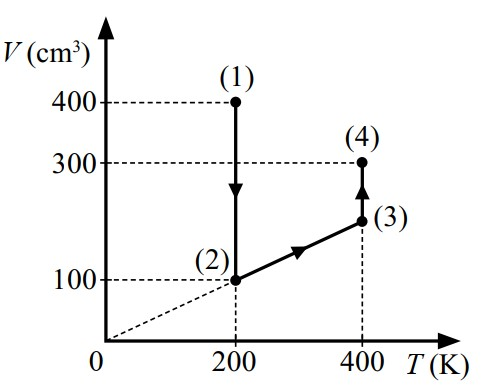
\includegraphics[width=0.35\linewidth]{../figs/G12C2-5}
	\end{center}
	\choiceTF[t]
	{\True $(1)\rightarrow (2)$ là quá trình nén đẳng nhiệt}
	{Áp suất của khối khí ở trạng thái (1) gấp 4 lần áp suất của khối khí ở trạng thái (2)}
	{Áp suất của khối khí ở trạng thái (4) gấp 1,5 lần áp suất của khối khí ở trạng thái (3)}
	{\True Ở trạng thái (2) và (3), khối khí có áp suất lớn nhất}
	\loigiai{}
\end{ex}
% ===================================================================
\begin{ex}
	Một quả bong bóng được thổi căng một phần và thả vào bên trong một chuông thuỷ tinh. Chuông được nối với một máy bơm chân không (hình bên dưới). Không khí trong chuông thuỷ tinh được máy bơm hút dần ra ngoài. Xem nhiệt độ của khí là không đổi.
	\begin{center}
		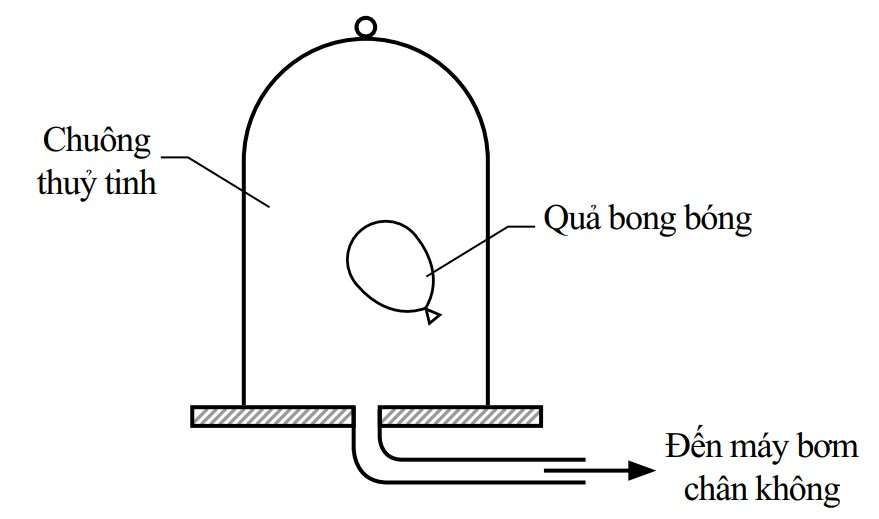
\includegraphics[width=0.4\linewidth]{../figs/G12C2-6}
	\end{center}
	\choiceTF[t]
	{\True Khi không khí được bơm dần ra ngoài thì áp suất không khí bên trong chuông giảm}
	{\True Khi không khí được bơm dần ra ngoài thì quả bong bóng dần căng phồng lên}
	{Quá trình căng phồng của quả bong bóng là quá trình dãn nở đẳng áp}
	{\True Khi quả bong bóng căng phồng lên, thể tích không khí bên trong quả bong bóng tăng lên và áp suất không khí bên trong quả bong bóng giảm}
	\loigiai{}
\end{ex}
% ===================================================================
\begin{ex}
	Một bình kín chứa $\SI{50}{\liter}$ khí oxygen ở $\SI{15}{\celsius}$ và áp suất $\SI{2.5E5}{\pascal}$.
	\choiceTF[t]
	{Lượng khí oxygen trong bình là $\SI{2.5}{\mole}$}
	{\True Thể tích của lượng khí trên ở điều kiện tiêu chuẩn xấp xỉ $\SI{117}{\liter}$}
	{\True Nếu đem bình ra phơi nắng để nhiệt độ khí trong bình tăng lên đến $\SI{49}{\celsius}$ thì áp suất khí trong bình khi đó xấp xỉ $\SI{2.8E5}{\pascal}$ (bỏ qua sự dãn nở vì nhiệt của bình chứa)}
	{Nếu mang bình đang đặt ngoài nắng vào trong nhà thì tốc độ chuyển động nhiệt của các phân tử khí trong bình tăng lên}
	\loigiai{}
\end{ex}
\Closesolutionfile{ans}
\section{Câu trắc nghiệm trả lời ngắn} \textit{Thí sinh trả lời từ câu 1 đến câu 6}
\setcounter{ex}{0}
% ===============================================================
\begin{ex}
	Một lượng khí lí tưởng thực hiện bốn quá trình như hình bên.
	Trong quá trình nào, áp suất của khí không đổi?
\begin{center}
	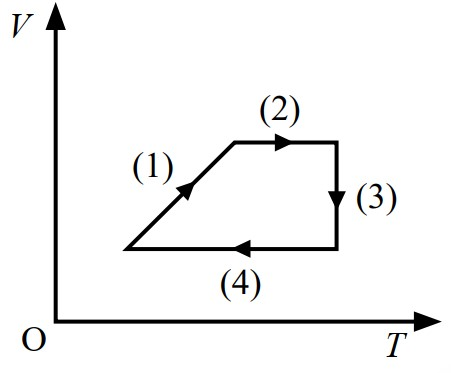
\includegraphics[width=0.25\linewidth]{../figs/G12C2-9}
\end{center}
	
	\shortans{1}
	\loigiai{
		
	}
\end{ex}
\Opensolutionfile{ans}[ans/Y24-VN12-PH-C2-TL]
% ===============================================================
\begin{ex}
	Khi đun nóng đẳng tích một khối khí thêm $\SI{1}{\celsius}$ thì áp suất khối khí tăng thêm $\dfrac{1}{360}$	áp suất ban đầu. Nhiệt độ ban đầu của khối khí đó là bao nhiêu $\si{\celsius}$?
	\shortans{87}
	\loigiai{
		$$\dfrac{p}{t+273}=\dfrac{p\left(1+\dfrac{1}{360}\right)}{t+274}\Rightarrow t=\SI{87}{\celsius}.$$
	}
\end{ex}
% ===============================================================
\begin{ex}
	Một bình có dung tích $\SI{4}{\liter}$ chứa một khối khí ở áp suất $\SI{2.4}{atm}$. Bình này được nối thông với một bình thứ hai có dung tích $\SI{8}{\liter}$ và được hút chân không. Xem nhiệt độ không đổi. Áp suất của khối khí sau khi hai bình được nối thông với nhau là bao nhiêu (tính theo đơn vị $\si{atm}$)?
	\shortans{0,8}
	\loigiai{
		$$p_1V_1=p_2\left(V_1+V_2\right)\Rightarrow p_2=\dfrac{2,4\cdot4}{12}=\SI{0.8}{atm}.$$
	}
\end{ex}
% ===============================================================
\begin{ex}
	Một lượng khí được chứa trong một xilanh được đậy kín bởi một pit-tông động như hình bên dưới. Ban đầu, độ dài phần xilanh chứa khí là $\SI{100}{\centi\meter}$, nhiệt độ khí là $\SI{27}{\celsius}$. Khi lượng khí được đun nóng đều thì pit-tông từ từ dịch chuyển cho đến khi độ dài phần xilanh chứa khí là $\SI{120}{\centi\meter}$. Nhiệt độ khí khi đó là bao nhiêu (tính theo đơn vị $\si{\celsius}$)?
	\begin{center}
		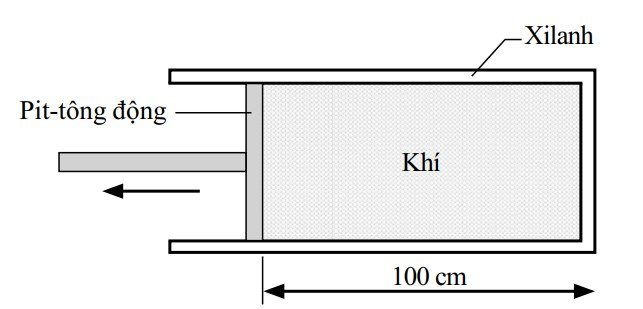
\includegraphics[width=0.4\linewidth]{../figs/G12C2-7}
	\end{center}
	\shortans{87}
	\loigiai{
		$$\dfrac{\ell_0S}{T_0}=\dfrac{\ell S}{T}\Leftrightarrow \dfrac{100}{27+273}=\dfrac{120}{t+273}\Rightarrow t=\SI{87}{\celsius}.$$
	}
\end{ex}
% ===============================================================
\begin{ex}
	Một khối khí thực hiện các quá trình biến đổi trạng thái như hình bên. Ở trạng thái (1), khối khí chiếm thể tích
	$\SI{1.2}{\liter}$. Xác định thể tích của khối khí ở trạng thái (3) (theo đơn vị $\si{\liter}$).
	\begin{center}
		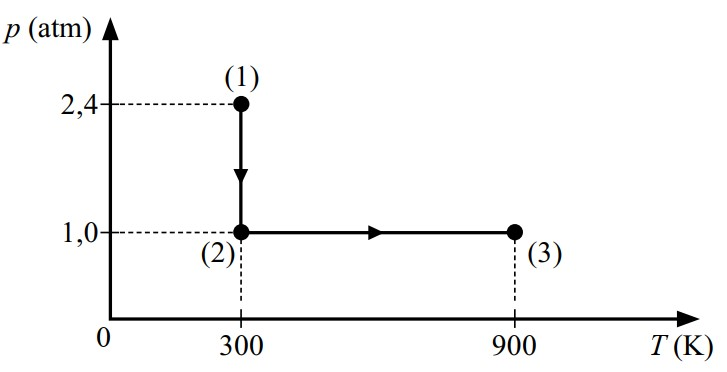
\includegraphics[width=0.4\linewidth]{../figs/G12C2-8}
	\end{center}
	\shortans{8,64}
	\loigiai{
	$$\dfrac{p_1V_1}{T_1}=\dfrac{p_2V_2}{T_2}\Leftrightarrow \dfrac{2,4\cdot1,2}{300}=\dfrac{1,0\cdot V_3}{900}\Rightarrow V_3=\SI{8.64}{\liter}.$$
	}
\end{ex}
%% ===============================================================
%\begin{ex}
%	Một khối khí chứa trong một bình đậy kín bằng một pit-tông động. Nhiệt độ và áp suất của khối khí lần lượt là $\SI{30}{\celsius}$ và $\SI{2.5E5}{\pascal}$. Pit-tông từ từ nén khối khí để thể tích khối khí giảm còn $\SI{10}{\percent}$ thể tích ban đầu thì thấy áp suất khối khí tăng lên đến $\SI{5.0E6}{\pascal}$. Nhiệt độ của khối khí biến thiên một lượng bao nhiêu $\si{\celsius}$?
%	\shortans{2.38}
%	\loigiai{
%		2.38
%	}
%\end{ex}
% ===============================================================
\begin{ex}
	Ở độ cao $h$, không khí có áp suất $\SI{230}{\milli\meter Hg}$ và nhiệt độ $\SI{-43}{\celsius}$. Xác định khối lượng riêng của không khí ở độ cao $h$ (theo đơn vị $\si{\kilogram/\meter^3}$, kết quả làm tròn đến hai chữ số
	thập phân). Giả sử ở mặt đất không khí có áp suất $\SI{760}{\milli\meter Hg}$, khối lượng riêng $\SI{1.22}{\kilogram/\meter^3}$,
	nhiệt độ $\SI{15}{\celsius}$.
	\shortans{0,46}
	\loigiai{
	$$\dfrac{D_2}{D_1}=\dfrac{V_1}{V_2}=\dfrac{p_2}{p_1}\cdot\dfrac{T_1}{T_2}\Rightarrow D_2=1,22\cdot\dfrac{230}{760}\cdot\left(\dfrac{15+273}{-43+273}\right)\approx\SI{0.46}{\kilogram/\meter^3}.$$
	}
\end{ex}
\Closesolutionfile{ans}
%	\stopcontents[mychapters]
%\stopcontents[parts]
%\fancyhf{}
%\part{ĐỀ KIỂM TRA GIỮA HỌC KÌ I}
\renewcommand{\thesection}{\Roman{section}}
\titleformat{\section}
{\normalfont\bfseries}{PHẦN~\thesection.}{0.4em}{}
	
%\chapter{Đề 1}
%\begin{tabular}{M{6.5cm}M{11cm}}
	\textbf{LỚP CÔ THẢO - THẦY SANG}& \textbf{ĐỀ ÔN TẬP KIỂM TRA GIỮA HỌC KÌ 1}\\
	\textbf{MÃ ĐỀ: 001}& \textbf{Bài thi môn: VẬT LÝ 12}\\
	\textit{(Đề trường Nguyễn Khuyến \newline Bình Dương năm học 2024 -2025)}& \textit{Thời gian làm bài: 50 phút, không kể thời gian phát đề}
	
	\noindent\rule{4cm}{0.8pt} \\
\end{tabular}
\setcounter{section}{0}
\begin{center}
	\textbf{\large BẢNG ĐÁP ÁN}
\end{center}
\section{}
\inputansbox{10}{ans/G12-1-TN}
\section{}
\inputansbox[2]{2}{ans/G12-1-TF}
\section{}
\inputansbox[3]{6}{ans/G12-1-TL}



\newpage
%\begin{tabular}{M{6.5cm}M{11cm}}
	\textbf{LỚP CÔ THẢO - THẦY SANG}& \textbf{ĐỀ ÔN TẬP KIỂM TRA GIỮA HỌC KÌ 1}\\
	\textbf{MÃ ĐỀ: 001}& \textbf{Bài thi môn: VẬT LÝ 12}\\
	\textit{(Đề trường Nguyễn Khuyến \newline Bình Dương năm học 2024 -2025)}& \textit{Thời gian làm bài: 50 phút, không kể thời gian phát đề}
	
	\noindent\rule{4cm}{0.8pt} \\
\end{tabular}
\setcounter{section}{0}
\section{Câu trắc nghiệm nhiều phương án lựa chọn}
\textit{Thí sinh trả lời từ câu 1 đến câu 18. Mỗi câu hỏi thí sinh chọn một phương án}
\setcounter{ex}{0}
\Opensolutionfile{ans}[ans/G12-1-TN]
% ===================================================================
\begin{ex}
	Một nhiệt kế thể tích không đổi hiển thị nhiệt độ $\SI{0}{\celsius}$ và $\SI{100}{\celsius}$ tương ứng với các áp suất $\SI{50}{\centi\meter Hg}$ và $\SI{90}{\centi\meter Hg}$. Biết nhiệt độ đọc được là hàm bậc nhất của áp suất. Khi áp suất thủy ngân là $\SI{60}{\centi\meter Hg}$ thì nhiệt độ đọc được bằng
	\choice
	{$\SI{35}{\celsius}$}
	{$\SI{30}{\celsius}$}
	{$\SI{20}{\celsius}$}
	{\True $\SI{25}{\celsius}$}
	\loigiai{
		$$\dfrac{t-t_b}{t_s-t_b}=\dfrac{p-p_b}{p_s-p_b}\Leftrightarrow \dfrac{t-0}{100-0}=\dfrac{60-50}{90-50}\Rightarrow t=\SI{25}{\celsius}.$$
	}
\end{ex}
% ===================================================================
\begin{ex}
	Chọn phát biểu \textbf{sai}? Sự bay hơi của một khối chất lỏng
	\choice
	{phụ thuộc vào diện tích mặt thoáng, diện tích mặt thoáng càng lớn thì sự bay hơi xảy ra càng nhanh}
	{xảy ra ở nhiệt độ bất kỳ}
	{phụ thuộc vào nhiệt độ, nhiệt độ càng cao sự bay hơi xảy ra càng nhanh}
	{\True phụ thuộc vào độ ẩm của không khí trên mặt thoáng, độ ẩm càng lớn thì sự bay hơi xảy ra càng nhanh}
	\loigiai{
		Độ ẩm càng bé thì sự bay hơi xảy ra càng nhanh.
	}
\end{ex}
% ===================================================================
\begin{ex}
	Để diệt trừ các bào tử nấm và kích thích quá trình nảy mầm của hạt giống lúa, người nông dân đã sử dụng một kinh nghiệm dân gian là ngâm chúng vào trong nước ấm theo công thức "hai sôi, ba lạnh". Tức là nước ấm ở nhiệt độ $T_{\mathrm{A}}\left(\si{\celsius}\right)$ sẽ được tạo ra bằng cách pha hai phần nước sôi $\left(\SI{100}{\celsius}\right)$ với ba phần nước lạnh $T_{\mathrm{L}}\left(\si{\celsius}\right)$. Chọn biểu thức đúng.
	\choice
	{$T_{\mathrm{A}}=\dfrac{200+3 T_{\mathrm{L}}}{2}$}
	{$T_{\mathrm{A}}=\dfrac{200+2 T_{\mathrm{L}}}{3}$}
	{\True $T_{\mathrm{A}}=\dfrac{200+3 T_{\mathrm{L}}}{5}$}
	{$T_{\mathrm{A}}=\dfrac{100+3 T_{\mathrm{L}}}{2}$}
	\loigiai{
		$$T_{\mathrm{A}}=\dfrac{m_scT_s+m_LcT_L}{m_sc+m_Lc}=\dfrac{2\cdot100+3T_L}{2+3}=\dfrac{200+3T_L}{5}.$$
	}
\end{ex}
% ===================================================================
\begin{ex}
	Nhiệt hóa hơi riêng có đơn vị đo là	
	\choice
	{$\si{\joule\cdot\kilogram/\kelvin}$}
	{$\si{\joule/\kilogram\cdot\kelvin}$}
	{\True $\si{\joule/\kilogram}$}
	{$\si{\joule}$}
	\loigiai{}
\end{ex}
% ===================================================================
\begin{ex}
	Chọn đáp án \textbf{sai}? Nhiệt hóa hơi riêng của chất lỏng phụ thuộc vào
	\choice
	{\True khối lượng của khối chất lỏng đó}
	{bản chất của khối chất lỏng đó (chất lỏng đó là chất gì, là nước hay dầu,\dots)}
	{nhiệt độ sôi của khối chất lỏng đó}
	{áp suất bề mặt của khối chất lỏng đó}
	\loigiai{}
\end{ex}
% ===================================================================
\begin{ex}
	Khi thép đang nóng chảy được làm nguội nhanh về nhiệt độ phòng sẽ giúp tăng độ cứng cho thép và cách làm như vậy được gọi là tôi thép. Người ta có thể sử dụng nước để làm hạ nhiệt độ nhanh cho thép đang nóng đỏ vì
	\choice
	{sử dụng nước là do thói quen vì thật ra có thể để thép nóng đỏ trong không khí thì thép cũng hạ nhanh về nhiệt độ phòng}
	{nhiệt độ nóng chảy của nước thấp hơn nhiều so với của thép}
	{\True nhiệt dung riêng của nước cao hơn nhiều so với của thép trong khi đó nhiệt độ sôi của nước lại thấp hơn nhiều so với nhiệt độ nóng chảy của thép}
	{nước có khả năng bốc hơi rất nhanh khi gặp kim loại nóng}
	\loigiai{}
\end{ex}
% ===================================================================
\begin{ex}
	Biểu thức diễn tả đúng độ biến thiên nội năng $\Delta U$ của chất khí trong quá trình chất khí vừa nhận nhiệt $Q$ vừa nhận công $A$ là?
	\choice
	{$\Delta U=A+Q$; $Q>0$; $A<0$}
	{$\Delta U=Q$; $Q>0$}
	{$\Delta U=Q+A$; $Q<0 $; $A>0$}
	{\True $\Delta U=Q+A$; $Q>0 $; $A>0$}
	\loigiai{}
\end{ex}
% ===================================================================
\begin{ex}
	Nước là chất có X lớn hơn nhiều so với các chất lỏng thông thường khác. Nhờ đó, nước có vai trò quan trọng đối với đời sống con người. Khoảng $\SI{70}{\percent}$ bề mặt của Trái Đất được bao phủ bởi nước. Nhờ có X lớn nên lượng nước này có thể hấp thụ lượng nhiệt khổng lồ của năng lượng mặt trời mà vẫn giữ cho nhiệt độ của bề mặt Trái Đất tăng không nhanh và không nhiều, tạo điều kiện thuận lợi cho sự sống của con người và các sinh vật khác. Cũng nhờ có X lớn mà nước biển nóng lên và nguội đi chậm hơn các vùng đất xung quanh. Do sự ổn định này của nhiệt độ nước biển mà các đảo và các vùng đất ven biển có khí hậu tương đối ôn hoà, thích hợp với con người. Cũng nhờ có X mà nước thường được dùng trong các thiết bị làm mát của động cơ nhiệt. Cụm từ tương ứng với X là
	\choice
	{nhiệt hóa hơi riêng}
	{nhiệt nóng chảy riêng}
	{khối lượng riêng}
	{\True nhiệt dung riêng}
	\loigiai{}
\end{ex}
% ===================================================================
\begin{ex}
	Khi làm muối, người ta đã dựa vào hiện tượng nào của nước?
	\choice
	{Sự sôi}
	{\True Bay hơi}
	{Đông đặc}
	{Ngưng tụ}
	\loigiai{}
\end{ex}
% ===================================================================
\begin{ex}
	Nhiệt hoá hơi riêng của một chất là nhiệt lượng cần cung cấp để $\SI{1}{\kilogram}$ chất đó
	\choice
	{hoá hơi hoàn toàn}
	{hoá hơi}
	{\True hoá hơi hoàn toàn ở nhiệt độ sôi}
	{bay hơi hết}
	\loigiai{}
\end{ex}
% ===================================================================
\begin{ex}
	Cho nhẹ nhàng vài viên đá vào một cốc nước. Sau một lúc ta thấy bên ngoài thành cốc có các giọt nước nhỏ li ti bám vào. Hiện tượng đó là do
	\choice
	{nước trong cốc thấm ra}
	{hơi nước trong không khí gặp lạnh ngưng kết lại}
	{\True hơi nước trong không khí gặp lạnh ngưng tụ}
	{nước trong cốc bay hơi và ngưng tụ lại}
	\loigiai{}
\end{ex}
% ===================================================================
\begin{ex}
	Ở thể khí, các phân tử ở (1) \dots Lực tương tác giữa các phân tử (2) \dots (trừ truờng hợp chúng va chạm nhau) nên các phân tử chuyển động hoàn toàn (3) \dots Do đó, khối chất khí không có (4) \dots.
	\choice
	{(1) gần nhau, (2) rất yếu, (3) trật tự, (4) hình dạng và thể tích riêng}
	{(1) gần nhau, (2) rất mạnh, (3) hỗn loạn, (4) hình dạng và thể tích riêng}
	{(1) xa nhau, (2) rất yếu, (3) hỗn loạn, (4) khối lượng và hình dạng}
	{\True (1) xa nhau, (2) rất yếu, (3) hỗn loạn, (4) hình dạng và thể tích riêng}
	\loigiai{}
\end{ex}
% ===================================================================
\begin{ex}
	Gọi lực liên kết giữa các phân tử trong chất rắn, chất lỏng, chất khí lần lượt là $F_{1}$, $F_{2}$, $F_{3}$ thì
	\choice
	{$F_{1}<F_{2}=F_{3}$}
	{$F_{1}=F_{2}=F_{3}$}
	{$F_{1}>F_{2}=F_{3}$}
	{\True $F_{1}>F_{2}>F_{3}$}
	\loigiai{}
\end{ex}
% ===================================================================
\begin{ex}
	Dùng một ca múc nước ở thùng chứa nước A có nhiệt độ $t_{\mathrm{A}}=\SI{20}{\celsius}$ và ở thùng chứa nước B ở nhiệt độ $t_{\mathrm{B}}=\SI{80}{\celsius}$ rồi đổ vào thùng nước C. Biết rằng trước khi đổ, trong thùng chứa nước C đã có sẵn một lượng nước ở nhiệt độ $t_{\mathrm{C}}=\SI{40}{\celsius}$ và bằng tổng số ca nước vừa mới đổ thêm vào nó. Bỏ qua sự trao đổi nhiệt với môi trường, với bình chứa và ca múc nước. Để có nhiệt độ nước ở thùng C là $\SI{50}{\celsius}$ thì số ca nước phải múc ở mỗi thùng A và B lần lượt là
	\choice
	{$3n$ ca và $2n$ ca}
	{\True $n$ ca và $2n$ ca}
	{$2n$ ca và $n$ ca}
	{$n$ ca và $3n$ ca}
	\loigiai{
		Áp dụng phương trình cân bằng nhiệt:
		\begin{eqnarray*}
			&&m_{\mathrm{A}}c\left(t_{\mathrm{cb}}-t_{\mathrm{A}}\right)+m_{\mathrm{B}}c\left(t_{\mathrm{cb}}-t_{\mathrm{B}}\right)+\left(m_{\mathrm{A}}+m_{\mathrm{B}}\right)c\left(t_{\mathrm{cb}}-t_{\mathrm{C}}\right)=0\\
			&\Rightarrow& m_{\mathrm{A}}\cdot\left(50-20\right)+m_{\mathrm{B}}\cdot\left(50-80\right)
			+\left(m_{\mathrm{A}}+m_{\mathrm{B}}\right)\cdot\left(50-40\right)=0\\
			&\Rightarrow& m_{\mathrm{B}}=2m_{\mathrm{A}}.
		\end{eqnarray*}
		
	}
\end{ex}
% ===================================================================
\begin{ex}
	Khi cho 2 vật chênh lệch nhiệt độ tiếp xúc nhau, năng lượng nhiệt luôn truyền từ vật có (1) \dots sang vật có (2) \dots Quá trình truyền nhiệt kết thúc khi hai vật (3) \dots (trạng thái này được gọi là trạng thái (4) \dots. Chọn đáp án có các cụm từ thích hợp điền vào chỗ trống.	
	\choice
	{(1) nhiệt độ thấp;	(2) nhiệt độ cao; (3) có cùng nội năng; (4) cân bằng nội năng}
	{\True (1) nhiệt độ cao;	(2) nhiệt độ thấp; (3) có cùng nhiệt độ; (4) cân bằng nhiệt}
	{(1) nhiệt độ thấp; (2) nhiệt độ cao; (3) có cùng nhiệt độ; (4) cân bằng nhiệt}
	{(1) nhiệt độ cao; (2) nhiệt độ thấp; (3) có cùng nội năng; (4) cân bằng nội năng}
	\loigiai{}
\end{ex}
% ===================================================================
\begin{ex}
	Một bạn học sinh làm thí nghiệm với đầy đủ thiết bị để xác định được nhiệt nóng chảy riêng của một chất khi đã biết nhiệt dung riêng của chất đó trong trạng thái rắn và trạng thái lỏng. Hãy chỉ ra phương án thí nghiệm sai trong các phương án sau.
	\choice
	{Bắt đầu thí nghiệm từ khi chất đó đang ở trạng thái rắn và kết thúc khi chất đó đã ở trạng thái lỏng}
	{\True Bắt đầu thí nghiệm từ khi chất đó đang ở trạng thái rắn và kết thúc khi đã thấy đã có sự nóng chảy của chất đó}
	{Thực hiện thí nghiệm từ khi chất bắt đầu đạt đến nhiệt độ nóng chảy nhưng chưa nóng chảy và kết thúc đo khi chất đó đã hoàn toàn ở trạng thái lỏng}
	{Thực hiện thí nghiệm từ khi chất đó bắt đầu đạt đến nhiệt độ nóng chảy nhưng chưa nóng chảy và kết thúc khi nóng chảy hoàn toàn và vẫn đang ở nhiệt độ nóng chảy}
	\loigiai{}
\end{ex}
% ===================================================================
\begin{ex}
	Nguyên nhân chính trong việc dùng wolfram để làm dây tóc trong bóng đèn sợi đốt là do wolfram
	\choice
	{có phân tử khối lớn}
	{mềm dễ làm sợi dây tóc}
	{là kim loại rất cứng}
	{\True có điểm nóng chảy cao}
	\loigiai{}
\end{ex}
% ===================================================================
\begin{ex}
	Sắp xếp các nhiệt độ sau. $\SI{37}{\celsius}$, $\SI{315}{\kelvin}$, $\SI{345}{\kelvin}$, $\SI{68}{\degree F}$ theo thứ tự tăng dần. Thứ tự đúng là
	\choice
	{\True $\SI{68}{\degree F}$, $\SI{37}{\celsius}$, $\SI{315}{\kelvin}$, $\SI{345}{\kelvin}$}
	{$\SI{37}{\celsius}$,  $\SI{315}{\kelvin}$, $\SI{345}{\kelvin}$, $\SI{68}{\degree F}$}
	{$\SI{315}{\kelvin}$,  $\SI{345}{\kelvin}$, $\SI{37}{\celsius}$, $\SI{68}{\degree F}$}
	{$\SI{68}{\degree F}$, $\SI{315}{\kelvin}$, $\SI{37}{\celsius}$, $\SI{345}{\kelvin}$}
	\loigiai{}
\end{ex}
\Closesolutionfile{ans}
\section{Câu trắc nghiệm đúng/sai} 
\textit{Thí sinh trả lời từ câu 1 đến câu 4. Trong mỗi ý \textbf{a)}, \textbf{b)}, \textbf{c)}, \textbf{d)} ở mỗi câu, thí sinh chọn đúng hoặc sai}
\setcounter{ex}{0}
\Opensolutionfile{ans}[ans/G12-1-TF]
% ===================================================================
\begin{ex}
	Tại điểm ba của nước,	
	\choiceTF[t]
	{\True hệ khảo sát có nhiệt độ theo thang Celsius là $\SI{0.01}{\celsius}$}
	{hệ khảo sát có áp suất $\SI{1}{atm}$}
	{\True nước tinh khiết tồn tại đồng thời ở cả ba thể rắn, lỏng, khí}
	{\True nhiệt độ của hệ khảo sát được chọn làm mốc trên thang đo Kelvin và có giá trị là $\SI{273.16}{\kelvin}$}
	\loigiai{
		\begin{itemchoice}
			\itemch Đúng.
			\itemch Sai. Hệ khảo sát có áp suất $\SI{0.006}{atm}$.
			\itemch Đúng.
			\itemch Đúng.
		\end{itemchoice}
	}
\end{ex}


% ===================================================================
\begin{ex}
	Trong thí nghiệm đo nhiệt nóng chảy riêng của nước đá, người ta sử dụng dòng điện để cung cấp nhiệt lượng cho $\SI{0.6}{\kilogram}$ nước đá trong nhiệt lượng kế. Dùng Oát kế đo được công suất dòng điện cung cấp là $\SI{930}{\watt}$, dùng đồng hồ để đo thời gian và nhiệt kế để đo nhiệt độ của khối nước. Đồ thị thực nghiệm đo được như hình.
	\begin{center}
		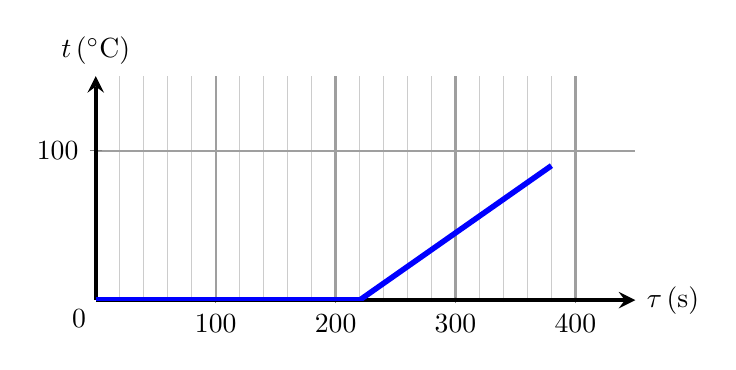
\begin{tikzpicture}  
			\begin{axis}[  ultra thick,yscale=0.5,
				xmin=0,  
				xmax=450,  
				xtick={0,100,200,300,400},
				ytick={0,100},
				minor x tick num=4,
				minor y tick num=0,
				ymin=0,  
				ymax=150, 
				samples=300,
				axis lines=center, 
				grid style={step=1, line width =0.4pt, color=gray!40!white},
				grid=both, %giới hạn ô lưới
				major grid style={line width=0.8pt,gray!75!white},
				xlabel=$\xsi{\tau}{\left(\si{\second}\right)}$, 		ylabel=$\xsi{t}{\left(\si{\celsius}\right)}$,
				every axis y label/.style={at=(current axis.above origin),anchor=south},  
				every axis x label/.style={at=(current axis.right of origin),anchor=west},  ]
				\addplot [line width=2pt, blue, smooth, domain=0:220] {0};  
				\addplot [line width=2pt, blue, smooth, domain=220:380] {0.5625*(x-220)}; 
				\coordinate (O) at (axis cs: 0,0);
			\end{axis}  
			\node[below left] at (O) {0};
		\end{tikzpicture}
	\end{center}
	\choiceTF[t]
	{\True Thời gian để nước đá tan hoàn toàn là $\SI{220}{\second}$}
	{\True Nếu hao phí nhiệt lượng là $\SI{2}{\percent}$, thì nhiệt nóng chảy riêng của nước đá là $\SI{334.18}{\kilo\joule/\kilogram}$}
	{Bỏ qua mọi hao phí thì nhiệt nóng chảy riêng của nước đá là $\SI{310}{\kilo\joule/\kilogram}$}
	{Trong giai đoạn từ thời điểm $\SI{0}{\second}$ đến $\SI{200}{\second}$, khối chất không nhận thêm nhiệt lượng}
	\loigiai{
		\begin{itemchoice}
			\itemch Đúng.
			\itemch Đúng. $H\calP t=m\lambda\Leftrightarrow 0,98\cdot930\cdot220=0,6\cdot\lambda\Rightarrow \lambda=\SI{334.18}{\kilo\joule/\kilogram}$.
			\itemch Sai. $\calP t=m\lambda\Leftrightarrow 930\cdot220=0,6\lambda\Rightarrow \lambda=\SI{341}{\kilo\joule/\kilogram}$.
			\itemch Sai. Từ thời điểm $\SI{0}{\second}$ đến $\SI{200}{\second}$, khối chất nhận nhiệt để nóng chảy.
		\end{itemchoice}
	}
\end{ex}
% ===================================================================
\begin{ex}
	Có hai chai nước lạnh A và B hoàn toàn giống nhau. Cho chai nước A vào chậu nước đến khi cân bằng nhiệt thì thấy nhiệt độ nước trong chậu giảm xuống. Lấy chai nước A ra ngoài và cho chai nước B vào chậu nước đến khi cân bằng nhiệt thì thấy nhiệt độ nước trong chậu tiếp tục giảm xuống, lấy chai B ra khỏi chậu nước. Xem như chỉ có sự trao đổi nhiệt giữa chai nước A, B và nước trong chậu.
	\choiceTF[t]
	{\True Sau khi lấy các chai nước ra khỏi chậu thì nhiệt độ của chai nước A cao hơn nhiệt độ của chai nước B}
	{Tổng độ tăng nhiệt độ của 2 chai nước bằng tổng độ giảm nhiệt độ của nước trong chậu ở 2 lần nhúng}
	{\True Độ giảm nhiệt độ của chậu nước trong lần nhúng chai nước A nhiều hơn lần nhúng chai nước	B}
	{Nhiệt lượng của chậu nước truyền cho hai chai nước là như nhau}
	\loigiai{
		\begin{itemchoice}
			\itemch Đúng.
			\begin{itemize}
				\item Thả chai nước A thì khi cân bằng nhiệt, nhiệt độ chai nước A bằng nhiệt độ $t_{\mathrm{cb1}}$ của nước trong chậu.
				\item Thả chai nước B thì khi cân bằng nhiệt, nhiệt độ chai nước B bằng nhiệt độ $t_{\mathrm{cb2}}$ của nước trong chậu.
				\item Mà nhiệt độ của nước trong chậu giảm xuống nên $t_{\mathrm{cb1}}>t_{\mathrm{cb2}}$.
			\end{itemize}
			\itemch Sai. Tổng độ tăng nội năng của 2 chai nước bằng tổng độ giảm nội năng của nước trong chậu.
			\itemch Đúng. \\
			$\begin{cases}
				m_Cc\left(t_C-t_1\right)=m_Ac\left(t_1-t_0\right)\\
				m_Cc\left(t_1-t_2\right)=m_Bc\left(t_2-t_0\right)
			\end{cases}\xrightarrow{m_A=m_B}\dfrac{t_C-t_1}{t_1-t_2}=\dfrac{t_1-t_0}{t_2-t_0}>1$.
			\itemch Sai. Nhiệt lượng chậu nước truyền cho chai A lớn hơn chai B.
		\end{itemchoice}
	}
\end{ex}
% ===================================================================
\begin{ex}
	Nhiệt kế rượu được chế tạo với thành phần chính của chất lỏng trong nhiệt kế là rượu. Một nhiệt kế rượu thông thường có giới hạn đo từ $\SI{-115}{\celsius}$ đến $\SI{78,5}{\celsius}$.
	\choiceTF[t]
	{\True Rượu được chọn làm nhiệt kế vì tính chất giãn nở đều theo nhiệt độ của nó}
	{\True Theo thang đo nhiệt độ Kelvin (làm tròn) thì giới hạn đo của nhiệt kế rượu kế trên là từ $\SI{158}{\kelvin}$ đến $\SI{351.5}{\kelvin}$}
	{Có thể dùng nhiệt kế rượu để đo nhiệt độ sôi của nước}
	{Hoàn toàn có thể dùng nước tinh khiết để thay thế cho rượu làm nhiệt kế}
	\loigiai{}
\end{ex}

\Closesolutionfile{ans}
\section{Câu trắc nghiệm trả lời ngắn} \textit{Thí sinh trả lời từ câu 1 đến câu 6}
\setcounter{ex}{0}
\Opensolutionfile{ans}[ans/G12-1-TL]
% ===============================================================
\begin{ex}
	Người ta cung cấp một nhiệt lượng $\SI{1.5}{\joule}$ cho chất khí đựng trong một xilanh đặt nằm ngang. Khí nở ra đẩy pittông di chuyển đều một đoạn $\SI{5}{\centi\meter}$. Biết lực ma sát giữa pittông và xilanh có độ lớn $\SI{20}{\newton}$. Xem như không có sự truyền nhiệt giữa khí và môi trường xung quanh. Tính độ biến thiên nội năng $\left(\si{\joule}\right)$ của khí trong xilanh?	
	\shortans{ 0,5}
	\loigiai{
		Công do khí thực hiện:
		$$A'=Fs=\left(\SI{20}{\newton}\right)\cdot\left(\SI{0.05}{\meter}\right)=\SI{1}{\joule}.$$
		Độ biến thiên nội năng của khí:
		$$\Delta U=Q+A=Q-A'=1,5-1=\SI{0.5}{\joule}.$$
	}
\end{ex}
% ===============================================================
\begin{ex}
	Một bình thuỷ tinh dung tích $\SI{20}{\liter}$ chứa $\SI{20}{\liter}$ khí oxygen. Nếu ta thêm vào bình $\SI{2}{\liter}$ khí oxygen nữa thì thể tích $\left(\si{\meter^3}\right)$ oxygen trong bình lúc này là bao nhiêu?
	\shortans{0,02 }
	\loigiai{
		Thể tích khí bằng thể tích bình chứa $V=\SI{20}{\liter}=\SI{0.02}{\meter^3}.$
	}
\end{ex}
% ===============================================================
\begin{ex}
	Rót khối lượng $m_{1}=\SI{0.5}{\kilogram}$ nước ở nhiệt độ $t_{1}=\SI{15}{\celsius}$ vào một bình nhiệt lượng kế có khối lượng $m_{2}=\SI{0.2}{\kilogram}$ đang ở nhiệt độ $t_{2}=\SI{30}{\celsius}$. Thả một cục nước đá có khối lượng $m_{3}=\SI{0.5}{\kilogram}$ ở nhiệt độ $t_{3}=\SI{-10}{\celsius}$ vào nước trong bình nhiệt lượng kế trên. Cho biết nhiệt dung riêng của nước, nước đá và bình nhiệt lượng kế tương ứng là $c_{1}=\SI{4.2E3}{\joule/\kilogram\cdot\kelvin}$; $c_{2}=\SI{2.1E3}{\joule/\kilogram\cdot\kelvin}$; $c_{3}=\SI{880}{\joule/\kilogram\cdot\kelvin}$; nhiệt nóng chảy của nước đá là $\lambda=\SI{3.3E5}{\joule/\kilogram}$. Bỏ qua sự trao đổi nhiệt với môi trường ngoài. Nhiệt độ $\left(\si{\celsius}\right)$ của hỗn hợp sau khi cân bằng nhiệt được thiết lập bằng bao nhiêu?
	\shortans{ 0}
	\loigiai{
		Nhiệt lượng nước và nhiệt lượng kế tỏa ra để giảm nhiệt độ xuống $\SI{0}{\celsius}$:
		$$Q_{\mathrm{tỏa}}=m_1c_1\left(t_1-0\right)+m_2c_3\left(t_2-0\right)=\SI{36.78}{\kilo\joule}.$$
		Nhiệt lượng nước đá thu vào để tăng nhiệt độ lên $\SI{0}{\celsius}$:
		$$Q_3=m_3c_2\left(0-t_3\right)=\SI{10.5}{\kilo\joule}.$$
		Nhiệt lượng nước đá cần thu vào để tan hoàn toàn:
		$$Q_{\mathrm{thu}}=m_3c_2\left(0-t_3\right)+m_3\lambda=\SI{175.5}{\kilo\joule}.$$
		Vì $Q_{\mathrm{thu}}>Q_{\mathrm{tỏa}}>Q_3$ nên nước đá chỉ tan một phần. Nhiệt độ cân bằng của hỗn hợp là $\SI{0}{\celsius}$.
		
	}
\end{ex}
% ===============================================================
\begin{ex}
	Người ta dùng bếp dầu hỏa để đun sôi nước, biết rằng phải tốn $\SI{150}{\gram}$ dầu hỏa mới đun sôi được $\SI{4.5}{\liter}$ nước ở $\SI{20}{\celsius}$, và cứ đốt $\SI{1}{\kilogram}$ dầu thì lượng nhiệt tỏa ra là $q=\SI{44E6}{\joule}$. Nhiệt dung riêng của nước là $\SI{4200}{\joule/\kilogram\cdot\kelvin}$, khối lượng riêng của nước là $\SI{1000}{\kilogram/\meter^3}$. Hiệu suất $\left(\si{\percent}\right)$ của bếp là bao nhiêu? (làm tròn đến 1 chữ số sau dấu phẩy)
	\shortans{22,9 }
	\loigiai{
		$$H=\dfrac{m_nc\Delta t}{m_dq}=\dfrac{DVc\Delta t}{m_dq}\approx\SI{22.9}{\percent}.$$
	}
\end{ex}
% ===============================================================
\begin{ex}
	Tại một đập thủy điện, người ta cho nước rơi từ độ cao $\SI{96}{\meter}$ xuống và đập vào cánh tuabin làm quay máy phát điện, biết rằng $\SI{50}{\percent}$ thế năng của nước làm nước nóng lên. Cho biết nhiệt dung riêng của nước là $\SI{4190}{\joule/\kilogram\cdot\kelvin}$. Lấy $g=\SI{10}{\meter/\second^2}$. Độ biến thiên nhiệt độ $\left(\si{\kelvin}\right)$ của nước là bao nhiêu? (làm tròn đến 1 chữ số sau dấu phẩy)
	\shortans{0,1 }
	\loigiai{
		$$\Delta t=\dfrac{mghH}{mc}=\dfrac{10\cdot96\cdot0,5}{4190}\approx\SI{0.1}{\kelvin}.$$
	}
\end{ex}
% ===============================================================
\begin{ex}
	Sự biến thiên nhiệt độ của khối nước đá đựng trong ca nhôm theo nhiệt lượng cung cấp được cho trên đồ thị. Cho nhiệt dung riêng của nước và nhôm lần lượt là $c_{1}=\SI{4200}{\joule/\kilogram\cdot\kelvin}$; $c_{2}=\SI{880}{\joule/\kilogram\cdot\kelvin}$, nhiệt nóng chảy của nước đá là $\lambda=\SI{3.4E5}{\joule/\kilogram}$. Khối lượng của ca nhôm bằng bao nhiêu $\si{\gram}$ (làm tròn đến phần nguyên)?
	\begin{center}
		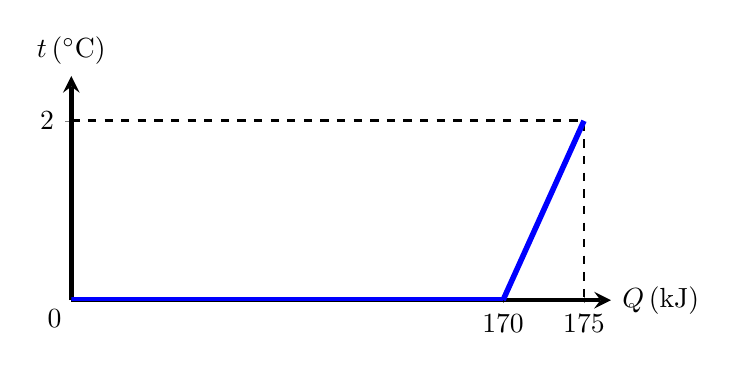
\begin{tikzpicture}  
			\begin{axis}[  ultra thick,yscale=0.5,
				xmin=0,  
				xmax=10,  
				xtick={0,8,9.5},
				ytick={0,2},
				ymin=0,  
				ymax=2.5, 
				samples=300,
				xticklabels={0,170,175},
				axis lines=center, 
				xlabel=$\xsi{Q}{\left(\si{\kilo\joule}\right)}$, 		ylabel=$\xsi{t}{\left(\si{\celsius}\right)}$,
				every axis y label/.style={at=(current axis.above origin),anchor=south},  
				every axis x label/.style={at=(current axis.right of origin),anchor=west},  ]
				\draw[dashed, line width=1pt] (axis cs: 0,2)--(axis cs: 9.5,2)--(axis cs: 9.5,0);
				\addplot [line width=2pt, blue, smooth, domain=0:8] {0};  
				\addplot [line width=2pt, blue, smooth, domain=8:9.5] {4*(x-8)/3};  
				\coordinate (O) at (0,0);
			\end{axis} 
			\node[below left] at (O) {0}; 
		\end{tikzpicture}
	\end{center}
	\shortans{455 }
	\loigiai{
		Khối lượng nước đá:
		$m_{\text{đ}}=\dfrac{\SI{170E3}{\joule}}{\lambda}=\SI{0.5}{\kilogram}.$\\
		Trong giai đoạn hệ tăng nhiệt độ:
		$$\left(m_{\text{đ}}c_1+mc_2\right)\cdot\Delta t=\SI{5E3}{\joule}\Rightarrow m\approx\SI{0.455}{\kilogram}=\SI{455}{\gram}.$$
	}
\end{ex}
\Closesolutionfile{ans}
\begin{center}
	\textbf{-- HẾT --}
\end{center}









%\chapter{Đề 2}
%\begin{tabular}{M{6.5cm}M{11cm}}
	\textbf{LỚP CÔ THẢO - THẦY SANG}& \textbf{ĐỀ ÔN TẬP KIỂM TRA GIỮA HỌC KÌ 1}\\
	\textbf{MÃ ĐỀ: 002}& \textbf{Bài thi môn: VẬT LÝ 12}\\
	\textit{(Đề trường TH - THCS - THPT\newline Lê Thánh Tông năm 2024 -2025)}& \textit{Thời gian làm bài: 50 phút, không kể thời gian phát đề}
	
	\noindent\rule{4cm}{0.8pt} \\
\end{tabular}
\setcounter{section}{0}
\begin{center}
	\textbf{\large BẢNG ĐÁP ÁN}
\end{center}
\section{}
\inputansbox{10}{ans/G12-2-TN}
\section{}
\inputansbox[2]{2}{ans/G12-2-TF}
\section{}
\inputansbox[3]{6}{ans/G12-2-TL}\newpage
%\begin{tabular}{M{6.5cm}M{11cm}}
	\textbf{LỚP CÔ THẢO - THẦY SANG}& \textbf{ĐỀ ÔN TẬP KIỂM TRA GIỮA HỌC KÌ 1}\\
	\textbf{MÃ ĐỀ: 002}& \textbf{Bài thi môn: VẬT LÝ 12}\\
	\textit{(Đề trường TH - THCS - THPT\newline Lê Thánh Tông năm 2024 -2025)}& \textit{Thời gian làm bài: 50 phút, không kể thời gian phát đề}
	
	\noindent\rule{4cm}{0.8pt} \\
\end{tabular}
\setcounter{section}{0}
\section{Câu trắc nghiệm nhiều phương án lựa chọn}
\textit{Thí sinh trả lời từ câu 1 đến câu 18. Mỗi câu hỏi thí sinh chọn một phương án}
\setcounter{ex}{0}
\Opensolutionfile{ans}[ans/G12-2-TN]
% ===================================================================
\begin{ex}
	Các vật không thể có nhiệt độ thấp hơn
	\choice
	{$\SI{2.0}{\kelvin}$}
	{$\SI{0}{\celsius}$}
	{$\SI{100}{\kelvin}$}
	{\True $\SI{-273.15}{\kelvin}$}
	\loigiai{}
\end{ex}
% ===================================================================
\begin{ex}
	Chọn câu đúng.	
	\choice
	{Khi một vật tỏa nhiệt ra môi trường thì nội năng của vật tăng lên}
	{Độ biến thiên nội năng của một vật là độ biến thiên nhiệt độ của vật đó}
	{\True Nội năng là phần năng lượng vật nhận được hay mất đi trong quá trình truyền nhiệt}
	{Nội năng của vật phụ thuộc vào nhiệt độ và thể tích của vật}
	\loigiai{}
\end{ex}
% ===================================================================
\begin{ex}
	Cho hai vật A và B tiếp xúc nhau. Nhiệt chỉ tự truyền từ A sang B khi
	\choice
	{A và B là hai vật rắn}
	{nhiệt độ của A và của B bằng nhau}
	{\True nhiệt độ của A lớn hơn nhiệt độ của B}
	{khối lượng của A lớn hơn khối lượng của B}
	\loigiai{}
\end{ex}
% ===================================================================
\begin{ex}
	Phát biểu nào dưới đây nói về nhiệt lượng là \textbf{không đúng}?	
	\choice
	{Nhiệt lượng là số đo độ biến thiên nội năng của vật trong quá trình truyền nhiệt}
	{\True Một vật lúc nào cũng có nội năng, do đó lúc nào cũng có nhiệt lượng}
	{Nhiệt lượng không phải là nội năng}
	{Đơn vị của nhiệt lượng cũng là đơn vị của nội năng}
	\loigiai{}
\end{ex}
% ===================================================================
\begin{ex}
	Trong quá trình chất khí nhận nhiệt lượng $Q$ và sinh công $A$, nội năng của một lượng khí biến thiên một lượng $\Delta U=A+Q$. Khi đó, $A$ và $Q$ phải thỏa mãn điều kiện nào dưới đây?
	\choice
	{$Q<0$ và $A>0$}
	{$Q<0$ và $A<0$}
	{\True $Q>0$ và $A<0$}
	{$Q>0$ và $A>0$}
	\loigiai{}
\end{ex}
% ===================================================================
\begin{ex}
	Câu nào sau đây nói về nội năng là \textbf{không đúng}?
	\choice
	{Nội năng của một hệ có thể tăng lên hoặc giảm xuống}
	{Nội năng là một dạng năng lượng}
	{Nội năng có thể chuyển hóa thành các dạng năng lượng khác}
	{\True Nội năng là nhiệt lượng}
	\loigiai{}
\end{ex}
% ===================================================================
\begin{ex}
	Chọn câu đúng.\\ 
	Trong quá trình hóa hơi một lượng chất lỏng ở nhiệt độ sôi
	\choice
	{\True nhiệt độ chất lỏng không thay đổi}
	{thể tích khối chất lỏng không thay đổi}
	{nhiệt độ của chất lỏng tăng liên tục}
	{nhiệt độ của chất lỏng giảm liên tục}
	\loigiai{}
\end{ex}
% ===================================================================
\begin{ex}
	Trong quá trình nóng chảy của nước đá đến khi nóng chảy hoàn toàn thì nhiệt độ của nước đá	
	\choice
	{tăng lên sau đó giảm xuống}
	{\True không thay đổi}
	{luôn giảm}
	{luôn tăng}
	\loigiai{}
\end{ex}
% ===================================================================
\begin{ex}
	Nếu làm tăng nhiệt độ của một hệ mà không làm thay đổi thể tích của nó thì nội năng của hệ sẽ
	\choice
	{\True tăng lên}
	{không thay đổi}
	{giảm xuống}
	{tăng lên sau đó giảm xuống}
	\loigiai{}
\end{ex}
% ===================================================================
\begin{ex}
	Phần năng lượng nhiệt mà vật này truyền cho vật kia hoặc vật này nhận từ vật kia gọi là	
	\choice
	{nội năng.}
	{thế năng}
	{nhiệt độ}
	{\True nhiệt lượng}
	\loigiai{}
\end{ex}
% ===================================================================
\begin{ex}
	Trường hợp nào dưới đây làm biến đổi nội năng \textbf{không phải} do thực hiện công?	
	\choice
	{Cọ xát hai vật vào nhau}
	{Nén khí trong xilanh}
	{\True Đun nóng nước bằng bếp}
	{Một viên bi bằng thép rơi xuống đất mềm}
	\loigiai{}
\end{ex}
% ===================================================================
\begin{ex}
	\immini{
		Hình bên là đường biểu diễn sự thay đổi nhiệt độ theo thời gian khi làm lạnh nước tinh khiết. Nhận định nào dưới đây là đúng?
		\choice
		{\True Từ phút thứ 5 tến phút thứ 6, nước ở cả thể lỏng và thể rắn}
		{Từ phút thứ nhất đến phút thứ hai, nước ở thể rắn}
		{Từ phút thứ 2 đến phút thứ 10 , nhiệt độ của nước không đổi}
		{Nhiệt độ của nước giảm đều theo thời gian}
	}
	{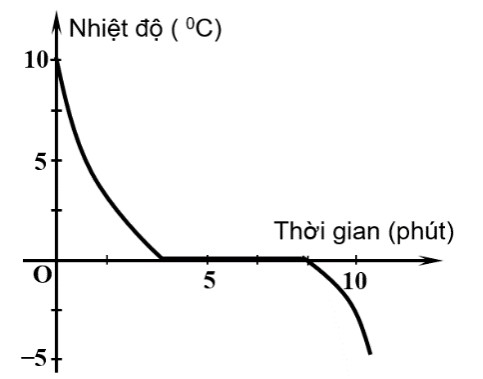
\includegraphics[width=0.6\linewidth]{../figs/D12-1-1}}
	\loigiai{}
\end{ex}
% ===================================================================
\begin{ex}
	Chiều cao của cột thủy ngân trong nhiệt kế thủy ngân thay đổi theo nhiệt độ. Ứng với hai vạch có nhiệt độ là $\SI{0}{\celsius}$ và $\SI{100}{\celsius}$ thì chiều cao của cột thủy ngân trong nhiệt kế là $\SI{2}{\centi\meter}$ và $\SI{22}{\centi\meter}$. Khi sử dụng nhiệt kế này để đo nhiệt độ của cơ thể của một em bé đang bị sốt thì thấy cột thủy ngân cao $\SI{9.9}{\centi\meter}$. Theo thang nhiệt Kelvin, nhiệt độ của em bé lúc này là bao nhiêu?
	\choice
	{$\SI{321.5}{\kelvin}$}
	{$\SI{305.5}{\kelvin}$}
	{$\SI{327.0}{\kelvin}$}
	{\True $\SI{312.5}{\kelvin}$}
	\loigiai{
		$$\dfrac{\ell -\ell_{\text{min}}}{\ell_{\text{max}}-\ell_{\text{min}}}=\dfrac{t -t_{\text{min}}}{t_{\text{max}}-t_{\text{min}}}\Leftrightarrow \dfrac{9,9-2}{22-2}=\dfrac{t-0}{100-0}\Rightarrow t=\SI{39.5}{\celsius}=\SI{312.5}{\kelvin}.$$
	}
\end{ex}
% ===================================================================
\begin{ex}
	Một viên đạn đại bác có khối lượng $\SI{10}{\kilogram}$ khi rơi tới đích có vận tốc $\SI{54}{\kilo\meter/\hour}$. Nếu toàn bộ động năng của nó biến thành nội năng thì nhiệt lượng tỏa ra lúc va chạm vào khoảng
	\choice
	{$\SI{14580}{\joule}$}
	{$\SI{2250}{\joule}$}
	{\True $\SI{1125}{\joule}$}
	{$\SI{7290}{\joule}$}
	\loigiai{
		$Q=\dfrac{1}{2}mv^2=\SI{1125}{\joule}$.
	}
\end{ex}
% ===================================================================
\begin{ex}
	Khi đun nóng một khối khí, khí giãn nở làm thể tích tăng thêm 7 lít. Biết trong quá trình này nội năng của khí giảm $\SI{1.1}{\kilo\joule}$ nhưng áp suất không đổi và bằng $\SI{3E5}{\pascal}$. Nhiệt lượng mà khối khí nhận được trong quá trình này là
	\choice
	{$\SI{3.2}{\kilo\joule}$}
	{\True $\SI{1.0}{\kilo\joule}$}
	{$\SI{1.5}{\kilo\joule}$}
	{$\SI{2.7}{\kilo\joule}$}
	\loigiai{
		Công khí thực hiện:
		$$A'=p\Delta V=\SI{2.1}{\kilo\joule}.$$
		Nhiệt lượng mà khối khí nhận được:
		$$Q=\Delta U-A=\Delta U+A'=-1,1+2,1=\SI{1.0}{\kilo\joule}.$$
	}
\end{ex}
% ===================================================================
\begin{ex}
	Hình bên là dự báo thời tiết ở thành phố Hồ Chí Minh ngày 21/07/2024. Theo thang nhiệt Kelvin, nhiệt độ cao nhất và thấp nhất theo bảng dự báo bên là
	\begin{center}
		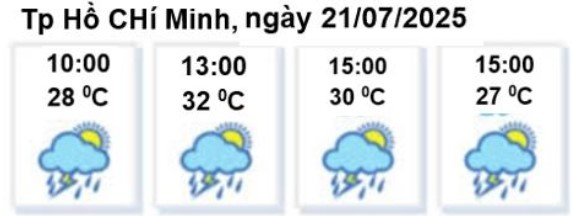
\includegraphics[width=0.3\linewidth]{../figs/D12-1-2}
	\end{center}
	\choice
	{$\SI{246}{\kelvin}$ và $\SI{241}{\kelvin}$}
	{\True $\SI{305}{\kelvin}$ và $\SI{300}{\kelvin}$}
	{$\SI{248}{\kelvin}$ và $\SI{236}{\kelvin}$}
	{$\SI{321}{\kelvin}$ và $\SI{306}{\kelvin}$}
	\loigiai{}
\end{ex}
% ===================================================================
\begin{ex}
	Một nhiệt kế có phạm vi đo từ $\SI{263}{\kelvin}$ đến $\SI{1273}{\kelvin}$, dùng để đo nhiệt độ của các lò nung. Phạm vi đo của nhiệt kế này trong thang nhiệt độ Celsius là
	\choice
	{$\SI{0}{\celsius}$ đến $\SI{273}{\celsius}$}
	{$\SI{-20}{\celsius}$ đến $\SI{1200}{\celsius}$}
	{\True $\SI{-10}{\celsius}$ đến $\SI{1000}{\celsius}$}
	{$\SI{-12}{\celsius}$ đến $\SI{1000}{\celsius}$}
	\loigiai{}
\end{ex}
% ===================================================================
\begin{ex}
	Khi nung nóng một lượng không khí chứa trong một xi lanh, khối khí nhận một nhiệt lượng $\SI{1.75}{\kilo\joule}$ làm nội năng của khí tăng thêm $\SI{720}{\joule}$. Khí giãn nở và sinh công làm pít - tông dịch chuyển. Khối khí đã thực hiện một công là	
	\choice
	{$\SI{2.56}{\kilo\joule}$}
	{\True $\SI{1.03}{\kilo\joule}$}
	{$\SI{1.25}{\kilo\joule}$}
	{$\SI{2.47}{\kilo\joule}$}
	\loigiai{
		$$A=\Delta U-Q=\SI{0.72}{\kilo\joule}-\SI{1.75}{\kilo\joule}=\SI{-1.03}{\kilo\joule}.$$
		Công khối khí thực hiện là $\SI{1.03}{\kilo\joule}$.
	}
\end{ex}
\Closesolutionfile{ans}
\section{Câu trắc nghiệm đúng/sai} 
\textit{Thí sinh trả lời từ câu 1 đến câu 4. Trong mỗi ý \textbf{a)}, \textbf{b)}, \textbf{c)}, \textbf{d)} ở mỗi câu, thí sinh chọn đúng hoặc sai}
\setcounter{ex}{0}
\Opensolutionfile{ans}[ans/G12-2-TF]
% ===================================================================
\begin{ex}
	Khi làm thí nghiệm đun nóng một chất. Kết quả thí nghiệm, một học sinh vẽ được biểu diễn sự thay đổi nhiệt độ của chất đó theo thời gian như hình bên.
	\begin{center}
		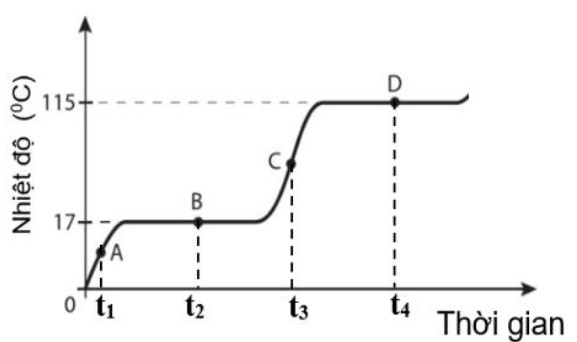
\includegraphics[width=0.4\linewidth]{../figs/D12-1-3}
	\end{center}
	\choiceTF[t]
	{Tại thời điểm $t_{2}$, chất ở thể lỏng}
	{\True Nhiệt độ nóng chảy của chất là $\SI{17}{\celsius}$}
	{Tại thời điểm $t_{3}$, chất ở thể rắn và thể lỏng}
	{\True Nhiệt độ sôi của chất này là $\SI{115}{\celsius}$}
	\loigiai{}
\end{ex}
% ===================================================================
\begin{ex}
	Có hai cốc nước A và B chứa cùng một lượng nước ở nhiệt độ phòng. Người ta thả một viên nước đá vào cốc A và nhúng cốc B vào một bình chứa nước nóng.
	\choiceTF[t]
	{\True Cốc B nhận nhiệt lượng từ nước ở bình, và nhiệt độ nước trong cốc tăng lên}
	{Nhiệt độ nước ở cốc A giảm vì nhận nhiệt lượng từ nước đá}
	{Nhiệt lượng không thể tự truyền từ nước ở cốc B vào nước ở bình chứa nó}
	{\True Khi nhiệt độ nước ở cốc B là $t_{2}=\SI{62}{\celsius}$ (theo thang nhiệt Celsius) thì theo thang nhiệt Kelvin là $T_{2} \approx \SI{335}{\kelvin}$}
	\loigiai{}
\end{ex}
% ===================================================================
\begin{ex}
	Đốt nóng khối khí trong xi lanh đặt nằm ngang bằng ngọn lửa đèn cồn như hình vẽ. Khí giãn nở đẩy pít - tông từ vị trí (1) đến vị trí (2).
	\begin{center}
		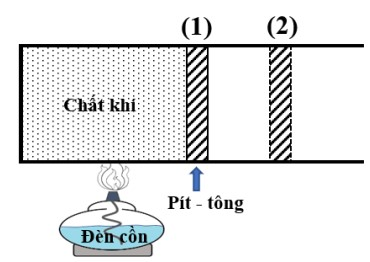
\includegraphics[width=0.3\linewidth]{../figs/D12-1-4}
	\end{center}
	\choiceTF[t]
	{\True Khối khí trong xi lanh nhận nhiệt lượng $Q\ (Q>0)$}
	{Khí dãn nở và nhận công $A\ (A>0)$}
	{\True Nội năng của khối khí khi pít - tông ở vị trí (2) là $\Delta U=Q+A$}
	{\True Khi khối khí trong xi lanh nhận được một nhiệt lượng $\SI{150}{\joule}$ thì khối khí giãn nở làm thể tích tăng từ $\SI{20}{\centi\meter^3}$ đến $\SI{30}{\centi\meter^3}$, biết rằng áp suất của khối khí trong xilanh không đổi và bằng $\SI{5E5}{\pascal}$. Nội năng của khối khí trong quá trình này tăng $\SI{145}{\joule}$}
	\loigiai{}
\end{ex}
% ===================================================================
\begin{ex}
	Các hình dưới đây là các đồ thị biểu diễn sự thay đổi thể tích $V$ phụ thuộc vào nhiệt độ $\left(\xsi{t}{\celsius}\right)$ trong quá trình nóng chảy của chì (H.1), của nước đá (H.2) và của sáp (nến) (H.3).	
	\begin{center}
		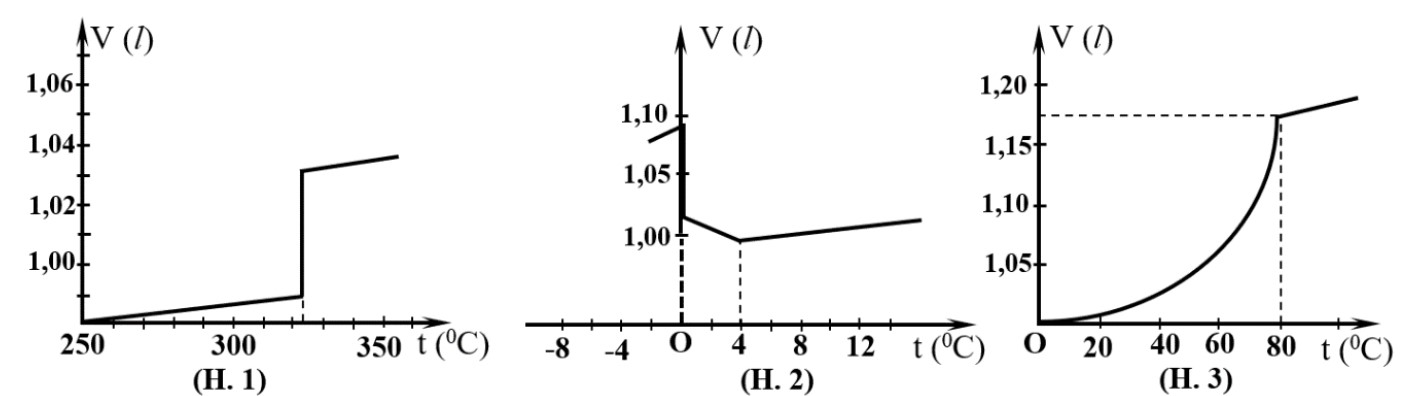
\includegraphics[width=0.9\linewidth]{../figs/D12-1-5}
	\end{center}
	\choiceTF[t]
	{Chì, nước đá và sáp (nến) đều có các nhiệt độ nóng chảy tương ứng nhất định}
	{Trong quá trình nóng chảy của chì, nước đá và sáp (nến) thể tích của chúng đều tăng tỉ lệ thuận với nhiệt độ}
	{\True Trong quá trình nóng chảy, nhiệt độ của chì và nước đá không thay đổi, còn nhiệt độ của sáp thay đổi liên tục}
	{\True Khi nóng chảy, chì và sáp (nến) dãn nở (thể tích $V$ tăng) còn nước đá co lại (thể tích $V$ giảm)}
	\loigiai{}
\end{ex}
\Closesolutionfile{ans}
\section{Câu trắc nghiệm trả lời ngắn} \textit{Thí sinh trả lời từ câu 1 đến câu 6}
\setcounter{ex}{0}
\Opensolutionfile{ans}[ans/G12-2-TL]
% ===============================================================
\begin{ex}
	Một lượng khí nhận một nhiệt lượng $\SI{35.40}{\kilo\joule}$ do được đun nóng, khí giãn ra và thực hiện một công $\SI{20.00}{\kilo\joule}$ ra môi trường xung quanh. Nội năng của khối khí này đã biến thiên một lượng bao nhiêu kilo joule $\left(\si{\kilo\joule}\right)$? \textit{(Kết quả lấy đến một chữ số sau dấu phẩy thập phân)}.	
	\shortans{15,4 }
	\loigiai{
		$\Delta U=Q+A=\SI{35.40}{\kilo\joule}-\SI{20.00}{\kilo\joule}=\SI{15.40}{\kilo\joule}$.
	}
\end{ex}
% ===============================================================
\begin{ex}
	Trong khoảng thời gian 2 phút 12 giây, nhiệt độ của một vật tăng từ $\SI{-15}{\celsius}$ đến $\SI{8.6}{\celsius}$. Nhiệt độ trung bình trong khoảng thời gian nói trên đã tăng bao nhiêu Kelvin/giây $\left(\si{\kelvin/\second}\right)$. \textit{(Kết quả lấy đến hai chữ số sau dấu phẩy thập phân)}.
	\shortans{0,33}
	\loigiai{
		$\dfrac{\Delta T}{\Delta t}=\dfrac{\SI{23.6}{\kelvin}}{\SI{72}{\second}}=\SI{0.33}{\kelvin/\second}.$
	}
\end{ex}
% ===============================================================
\begin{ex}
	Một khối khí được cung cấp nhiệt lượng $\SI{4.98}{\kilo\joule}$, khí giãn nở làm tăng thể tích một lượng $\xsi{\Delta V}{\deci\meter^3}$. Trong quá trình này, nội năng của khối khí biến thiên $\SI{1.23}{\kilo\joule}$ nhưng áp suất của khối khí không đổi và bằng $p=\SI{2.5E5}{\pascal}$. Giá trị của $\Delta \mathrm{V}$ là bao nhiêu?	
	\shortans{15 }
	\loigiai{
		$\Delta U=Q-p\Delta V\Rightarrow \Delta V=\SI{0.015}{\meter^3}=\SI{15}{\deci\meter^3}$.
	}
\end{ex}
% ===============================================================
\begin{ex}
	Một vật có khối lượng $\SI{2}{\kilogram}$ trượt không vận tốc đầu từ đỉnh xuống chân một mặt nghiêng dài $\SI{40}{\meter}$, nghiêng một góc $\SI{60}{\degree}$ so với phương ngang. Tốc độ của vật ở chân mặt phẳng nghiêng là $\SI{4.5}{\meter/\second}$. Cho rằng, $\SI{75}{\percent}$ công của lực ma sát giữa mặt phẳng nghiêng và vật chuyển thành nội năng của vật, bỏ qua phần nhiệt lượng mặt phẳng nghiêng truyền cho vật. Lấy $g=\SI{9.8}{\meter/\second^2}$. Độ biến thiên nội năng của vật trong quá trình trên là bao nhiêu kilo joule $\left(\si{\kilo\joule}\right)$. \textit{(Kết quả lấy đến hai chữ số sau dấu phẩy thập phân)}.
	\shortans{0,49 }
	\loigiai{
		$h=\ell\sin\alpha=\xsi{20\sqrt{3}}{\meter}$.\\
		Công lực ma sát:
		$$\left|A_{\text{ms}}\right|=W_1-W_2=mgh-\dfrac{1}{2}mv^2\approx\SI{658.7}{\joule}.$$
		Độ biến thiên nội năng của vật:
		$$\Delta U=0,75\left|A_{\text{ms}}\right|\approx\SI{0.49}{\kilo\joule}.$$
	}
\end{ex}
% ===============================================================
\begin{ex}
	Một xi lanh có pít - tông nằm ngang như hình vẽ, xilanh chứa $\SI{500}{\centi\meter^3}$ không khí. Khi đốt nóng khí trong xi lanh, khí giãn nở đẩy pít - tông qua phải làm thể tích khối khí tăng lên $\SI{720}{\centi\meter^3}$, nội năng khối khí tăng thêm $\SI{1.5}{\kilo\joule}$. Cho rằng áp suất của khối khí luôn bằng $5,8 \cdot 10^{5} \mathrm{~Pa}$. Nhiệt lượng đã cung cấp cho khối khí bao nhiêu kilôjun (kJ). \textit{(Kết quả lấy đến hai chữ số sau dấu phẩy thập phân)}.
	\begin{center}
		\includegraphics[width=0.3\linewidth]{../figs/D12-1-6}
	\end{center}
	\shortans{1,63 }
	\loigiai{
		Công khí thực hiện:
		$$A'=p\Delta V=\left(\SI{5.8E5}{\pascal}\right)\cdot\left(\SI{720E-6}{\meter^3}-\SI{500E-6}{\meter^3}\right)=\SI{127.6}{\joule}.$$
		Nhiệt lượng đã cung cấp cho khí:
		$$Q=\Delta U-A=\Delta U+A'=	\SI{1.63}{\kilo\joule}.$$
	}
\end{ex}
% ===============================================================
\begin{ex}
	Hiện nay, người ta có thể dùng các vỉ đá được làm nóng sẵn trong lò (tăng nội năng của vỉ đá) để nướng thức ăn. Giả sử, một vỉ đá có khối lượng $\SI{1.2}{\kilogram}$, nhiệt độ ban đầu là $\SI{28}{\celsius}$ được làm nóng trong lò có công suất $\SI{20}{\kilo\watt}$. Coi như toàn bộ năng lượng của lò cung cấp sẽ dùng để làm nóng vỉ đá. Biết rằng, để làm cho $\SI{1}{\kilogram}$ đá làm vỉ này tăng thêm $\SI{1}{\celsius}$ thì cần nhiệt lượng $\SI{5500}{\joule}$. Để vỉ đá đạt được nhiệt độ $\SI{1000}{\celsius}$ thì cần thời gian bao nhiêu phút? \textit{(Kết quả lấy đến hai chữ số sau dấu phẩy thập phân)}.
	\shortans{5.35 }
	\loigiai{
		$t=\dfrac{mc\Delta t}{\calP}=\dfrac{\left(\SI{1.2}{\kilogram}\right)\cdot\left(\SI{5500}{\joule/\kilogram\cdot\kelvin}\right)\cdot\left(\SI{1000}{\celsius}-\SI{28}{\celsius}\right)}{\SI{20E3}{\watt}}=\SI{320.76}{\second}\approx\SI{5.35}{\minute}.$
	}
\end{ex}
\Closesolutionfile{ans}
\begin{center}
	\textbf{-- HẾT --}
\end{center}
%\chapter{Đề 3}
%\begin{tabular}{M{6.5cm}M{11cm}}
	\textbf{LỚP CÔ THẢO - THẦY SANG}& \textbf{ĐỀ ÔN TẬP KIỂM TRA GIỮA HỌC KÌ 1}\\
	\textbf{MÃ ĐỀ: 003}& \textbf{Bài thi môn: VẬT LÝ 12}\\
	\textit{(Đề trường TH - THCS - THPT\newline Lê Thánh Tông năm 2024 -2025)}& \textit{Thời gian làm bài: 50 phút, không kể thời gian phát đề}
	
	\noindent\rule{4cm}{0.8pt} \\
\end{tabular}
\setcounter{section}{0}
\begin{center}
	\textbf{\large BẢNG ĐÁP ÁN}
\end{center}
\section{}
\inputansbox{10}{ans/G12-3-TN}
\section{}
\inputansbox[2]{2}{ans/G12-3-TF}
\section{}
\inputansbox[3]{6}{ans/G12-3-TL}\newpage
%\begin{tabular}{M{6.5cm}M{11cm}}
	\textbf{TRUNG TÂM MANABIE}& \textbf{ĐỀ ÔN TẬP KIỂM TRA GIỮA HỌC KÌ 1}\\
	\textbf{MÃ ĐỀ: 003}& \textbf{Bài thi môn: VẬT LÝ 12}\\
	\textit{(Đề trường TH - THCS - THPT\newline Lê Thánh Tông năm 2024 -2025)}& \textit{Thời gian làm bài: 50 phút, không kể thời gian phát đề}
	
	\noindent\rule{4cm}{0.8pt} \\
\end{tabular}
\setcounter{section}{0}
\section{Câu trắc nghiệm nhiều phương án lựa chọn}
\textit{Thí sinh trả lời từ câu 1 đến câu 18. Mỗi câu hỏi thí sinh chọn một phương án}
\setcounter{ex}{0}
\Opensolutionfile{ans}[ans/G12-3-TN]
% ===================================================================
\begin{ex}
	Nhiệt lượng mà một vật đồng chất thu vào để tăng nhiệt độ thêm $\SI{40}{\celsius}$ là $\SI{17.6}{\kilo\joule}$. Bỏ qua sự trao đổi nhiệt với môi trường. Biết khối lượng của vật là $\SI{500}{\gram}$, nhiệt dung riêng của chất làm vật là	
	\choice
	{$\SI{112.5}{\joule/\kilogram\cdot\kelvin}$}
	{$\SI{460}{\joule/\kilogram\cdot\kelvin}$}
	{$\SI{380}{\joule/\kilogram\cdot\kelvin}$}
	{\True $\SI{880}{\joule/\kilogram\cdot\kelvin}$}
	\loigiai{$c=\dfrac{Q}{m\Delta t}=\SI{880}{\joule/\kilogram\cdot\kelvin}$}
\end{ex}
% ===================================================================
\begin{ex}
	Trường hợp nào dưới đây làm biến đổi nội năng của vật không phải do thực hiện công?
	\choice
	{Khuấy nước}
	{Mài dao}
	{\True Nung đồng trong lò}
	{Đóng đinh}
	\loigiai{}
\end{ex}
% ===================================================================
\begin{ex}
	Chọn phát biểu đúng về sự nóng chảy của một chất nào đó.
	\choice
	{\True Cần cung cấp nhiệt lượng}
	{Xảy ra ở cùng nhiệt độ với sự hoá hơi}
	{Xảy ra ở $\SI{100}{\celsius}$}
	{Toả nhiệt ra môi trường}
	\loigiai{}
\end{ex}
% ===================================================================
\begin{ex}
	Một thước $\si{\centi\meter}$ được đặt dọc theo một nhiệt kế thủy ngân chưa được chia vạch như hình dưới đây. Trên nhiệt kế chỉ đánh dấu điểm đóng băng và điểm sôi của nước tinh khiết ở áp suất tiêu chuẩn. Giá trị nhiệt độ đang hiển thị trên nhiệt kế là bao nhiêu?
	\begin{center}
		\includegraphics[width=0.5\linewidth]{../figs/D12-2-1}
	\end{center}
	\choice
	{\True $\SI{56}{\celsius}$}
	{$\SI{60}{\celsius}$}
	{$\SI{66}{\celsius}$}
	{$\SI{44}{\celsius}$}
	\loigiai{
		$\dfrac{t-t_b}{t_s-t_b}=\dfrac{\ell-\ell_b}{\ell_s-\ell_b}\Leftrightarrow \dfrac{t-0}{100-0}=\dfrac{6,6-1}{11-1}\Rightarrow t=\SI{56}{\celsius}.$
	}
\end{ex}
% ===================================================================
\begin{ex}
	Một căn phòng có thể tích $\SI{50}{\meter^3}$. Khi tăng nhiệt độ của phòng từ $\SI{20}{\celsius}$ đến $\SI{30}{\celsius}$ thì khối lượng không khí (coi là khí lí tưởng) thoát ra khỏi căn phòng là bao nhiêu kilogram? Coi áp suất khí trong phòng không đổi. Biết khối lượng riêng của không khí ở $\SI{20}{\celsius}$ là $\SI{1.2}{\kilogram/\meter^3}$.	
	\choice
	{\True $\SI{1.98}{\kilogram}$}
	{$\SI{30.00}{\kilogram}$}
	{$\SI{2.05}{\kilogram}$}
	{$\SI{1.98}{\kilogram}$}
	\loigiai{
		Trong điều kiện áp suất không đổi:
		$$\dfrac{D_2}{D_1}=\dfrac{V_1}{V_2}=\dfrac{T_1}{T_2}\Rightarrow D_2\approx\SI{1.16}{\kilogram/\meter^3}$$
		Khối lượng không khí thoát ra khỏi căn phòng:
		$$\Delta m=m_1-m_2=\left(D_1-D_2\right)V=\SI{1.98}{\kilogram}.$$
	}
\end{ex}
% ===================================================================
\begin{ex}
	\immini{
		Hình bên là đồ thị biểu diễn sự phụ thuộc của áp suất $p$ theo thể tích $V$ khi nhiệt độ không đổi của một lượng khí lí tưởng xác định. Gọi $S_{1}$ và $S_{2}$ lần lượt là diện tích của các hình chữ nhật ABCD và DEFG. Hệ thức đúng giữa $S_{1}$ và $S_{2}$ là
		\choice
		{$S_{1}>S_{2}$}
		{$3 S_{1}=2 S_{2}$}
		{$S_{1}<S_{2}$}
		{\True $S_{1}=S_{2}$}
	}
	{
		\includegraphics[width=0.5\linewidth]{../figs/D12-2-2}
	}
	\loigiai{
		Quá trình biến đổi từ G$\rightarrow$ C là đẳng nhiệt nên $p_{\mathrm{G}}V_{\mathrm{G}}=p_{\mathrm{C}}V_{\mathrm{C}}\Rightarrow S_{\mathrm{BCEO}}=S_{\mathrm{AGFO}}\Rightarrow S_{\mathrm{ABCD}}=S_{\mathrm{EFGD}}$.
	}
\end{ex}
% ===================================================================
\begin{ex}
	Trong một quá trình biến đổi, nội năng của một khối khí giảm đi $\SI{15}{\joule}$. Nếu trong quá trình đó khối khí nhận vào một nhiệt lượng là $\SI{35}{\joule}$ thì khối khí đã 
	\choice
	{sinh công $\SI{20}{\joule}$}
	{nhận công $\SI{50}{\joule}$}
	{nhận công $\SI{20}{\joule}$}
	{\True sinh công $\SI{50}{\joule}$}
	\loigiai{
		$\Delta U=Q+A\Rightarrow A=\Delta U-Q=-15-35=\SI{-50}{\joule}.$
	}
\end{ex}
% ===================================================================
\begin{ex}
	\immini{
		Một khối khí lí tưởng xác định biến đổi theo các quá trình (1) - (2) - (3) - (4) như hình vẽ. Cho $p$ là áp suất và $V$ là thể tích của khối khí. Biết nhiệt độ của khối khí ở trạng thái (4) là $\SI{-153}{\celsius}$. Nhiệt độ của khối khí này ở trạng thái (1) là
		\choice
		{$\SI{960}{\celsius}$}
		{\True $\SI{687}{\celsius}$}
		{$\SI{1224}{\celsius}$}
		{$\SI{1233}{\celsius}$}
		
	}
	{
		\includegraphics[width=0.55\linewidth]{../figs/D12-2-3}
	}
	\loigiai{
		$$\dfrac{p_1V_1}{T_1}=\dfrac{p_4V_4}{T_4}\Leftrightarrow \dfrac{4\cdot2}{T_1}=\dfrac{1\cdot1}{-153+273}\Rightarrow T_1=\SI{960}{\kelvin}\Rightarrow t_1=\SI{687}{\celsius}.$$
	}
\end{ex}

% ===================================================================
\begin{ex}
	Một ống thủy tinh tiết diện đều một đầu kín, một đầu hở, chiều dài $L=\SI{50}{\centi\meter}$, có một cột thủy ngân dài $H =\SI{19}{\centi\meter}$ bịt kín một cột không khí trong ống. Coi nhiệt độ không đổi. Khi đặt ống thủy tinh nằm ngang thì chiều dài cột không khí là $L_1=\SI{20}{\centi\meter}$. Khi đặt ống thủy tinh thẳng đứng với đầu hở ở trên thì chiều dài cột không khí là $L_2=\SI{16}{\centi\meter}$. Nếu ống thủy tinh được đặt thẳng đứng với đầu hở ở dưới thì chiều dài của cột không khí bên trong ống là
	\choice
	{$\SI{22.12}{\centi\meter}$}
	{$\SI{50.00}{\centi\meter}$}
	{$\SI{25.73}{\centi\meter}$}
	{$\SI{26.67}{\centi\meter}$}
	\loigiai{
		$$p_0L_1=\left(p_0+H\right)L_2=\left(p_0-H\right)L_3\Rightarrow \begin{cases}
			p_0=\SI{76}{\centi\meter Hg}\\
			L_3\approx\SI{26.67}{\centi\meter}
		\end{cases}.$$
	}
\end{ex}
% ===================================================================
\begin{ex}
	Hàn thiếc là một phương pháp nối kim loại với nhau bằng một kim loại hay hợp kim trung gian (thiếc) gọi là vảy hàn. Trong quá trình nung nóng để hàn, vảy hàn sẽ nóng chảy trước trong khi vật hàn chưa nóng chảy hoặc nóng chảy với số lượng không đáng kể. Khi đó kim loại làm vảy hàn sẽ khuếch tán thẩm thấu vào trong kim loại vật hàn tạo thành mối hàn. Thiếc hàn là hợp kim	thiếc - chì có nồng độ phù hợp với mục đích sử dụng. Ví dụ thiếc hàn 60 ($\SI{60}{\percent}\ \ce{Sn}$ và $\SI{40}{\percent}
	\ \ce{Pb}$) được sử dụng để hàn các dây dẫn hay mối nối trong mạch điện. Thiếc hàn phải có
	\choice
	{nhiệt độ nóng chảy và nhiệt nóng chảy riêng lớn hơn của kim loại vật hàn}
	{nhiệt độ nóng chảy lớn để tránh nóng chảy mối hàn trong quá trình sử dụng}
	{\True nhiệt độ nóng chảy và nhiệt nóng chảy riêng nhỏ hơn của kim loại vật hàn}
	{nhiệt nóng chảy riêng lớn để tránh nóng chảy mối hàn trong quá trình sử dụng}
	\loigiai{
		Vảy hàn phải có nhiệt độ nóng chảy và nhiệt dung riêng nhỏ hơn vật hàn để nóng chảy trước.
	}
\end{ex}
% ===================================================================
\begin{ex}
	Cho $p$ là áp suất, $V$ là thể tích, $T$ là nhiệt độ tuyệt đối của một lượng khí lí tưởng xác định. Hình nào dưới đây biểu diễn quá trình biến đổi trạng thái của lượng khí đó khác với các hình còn lại?
	\begin{center}
		\includegraphics[width=0.7\linewidth]{../figs/D12-2-4}
	\end{center}
	\choice
	{Hình 3}
	{Hình 4}
	{Hình 2}
	{\True Hình 1}
	\loigiai{
		Hình 1 là quá trình đẳng tích, các hình còn lại là quá trình đẳng áp.
	}
\end{ex}
% ===================================================================
\begin{ex}
	Trong thí nghiệm kiểm chứng lại định luật Boyle, việc dịch chuyển pit-tông từ từ giúp đảm bảo điều kiện gì?
	\begin{center}
		\includegraphics[width=0.3\linewidth]{../figs/D12-2-5}
	\end{center}
	\choice
	{Áp suất không đổi}
	{\True Nhiệt độ không đổi}
	{Thể tích không đổi}
	{Nhiệt độ và áp suất không đổi}
	\loigiai{}
\end{ex}
% ===================================================================
\begin{ex}
	Phát biểu nào sau đây về nội năng là \textbf{không đúng}?
	\choice
	{Nội năng là một dạng năng lượng}
	{Nội năng của một vật có thể tăng hoặc giảm}
	{\True Nội năng là nhiệt lượng}
	{Nội năng có thể chuyển hoá thành các dạng năng lượng khác}
	\loigiai{}
\end{ex}
% ===================================================================
\begin{ex}
	Với cùng một chất, quá trình chuyển thể nào sẽ làm giảm lực tương tác giữa các phân tử nhiều nhất?
	\choice
	{\True Hoá hơi}
	{Đông đặc}
	{Nóng chảy}
	{Ngưng tụ}
	\loigiai{}
\end{ex}
% ===================================================================
\begin{ex}
	Đơn vị nào sau đây không phải là đơn vị đo áp suất?
	\choice
	{$\si{\milli\meter Hg}$}
	{\True $\si{HP}$}
	{$\si{bar}$}
	{$\si{\newton/\meter^2}$}
	\loigiai{}
\end{ex}
% ===================================================================
\begin{ex}
	Nội dung nào dưới đây \textbf{không phải} là sự thể hiện của hiện tượng bay hơi của vật chất?
	\choice
	{Bật quạt sau khi lau sàn nhà}
	{\True Xuất hiện các giọt nước ở thành ngoài cốc nước giải khát có đá khi để trong không khí}
	{Sử dụng khí gas ($\ce{R}-32$) trong các thiết bị làm lạnh của máy điều hoà không khí}
	{Sản xuất muối của các diêm dân}
	\loigiai{}
\end{ex}
% ===================================================================
\begin{ex}
	Khi đi tham quan trên các vùng núi cao có nhiệt độ thấp hơn nhiều dưới đồng bằng, chúng ta cần mang theo áo ấm để sử dụng vì
	\choice
	{mặc áo ấm để ngăn hơi lạnh truyền vào trong cơ thể}
	{mặc áo ấm để ngăn nhiệt độ cơ thể truyền ra ngoài môi truờng}
	{\True mặc áo ấm để ngăn cơ thể mất nhiệt lượng quá nhanh}
	{mặc áo ấm để ngăn tia cực tím từ Mặt Trời}
	\loigiai{}
\end{ex}
% ===================================================================
\begin{ex}
	Chuyển động nào sau đây không được coi là chuyển động Brown?
	\choice
	{Chuyển động của các hạt bụi lơ lửng trong không khí khi quan sát dưới ánh nắng mặt trời vào buổi sáng}
	{Chuyển động của hạt phấn hoa trong nước}
	{Chuyển động của các hạt mực khi nhỏ các giọt mực vào nước}
	{\True Chuyển động thành dòng của các hạt bụi nhỏ trong ống khói của nhà máy xi măng đang vận hành}
	\loigiai{}
\end{ex}
\Closesolutionfile{ans}
\section{Câu trắc nghiệm đúng/sai} 
\textit{Thí sinh trả lời từ câu 1 đến câu 4. Trong mỗi ý \textbf{a)}, \textbf{b)}, \textbf{c)}, \textbf{d)} ở mỗi câu, thí sinh chọn đúng hoặc sai}
\setcounter{ex}{0}
\Opensolutionfile{ans}[ans/G12-3-TF]
% ===================================================================
\begin{ex}
	\immini{Một mô hình áp kế khí ở hình bên gồm một bình cầu thuỷ tinh có thể tích $\SI{270}{\centi\meter^3}$ gắn với một ống nhỏ AB nằm ngang có tiết diện $\SI{0.1}{\centi\meter^2}$. Trong ống có một giọt thuỷ ngân. Ở $\SI{0}{\celsius}$ giọt thuỷ ngân cách A $\SI{30}{\centi\meter}$. }
	{\includegraphics[width=0.5\linewidth]{../figs/D12-2-6}
		
	}
	Sau đó người ta hơ nóng bình cầu để	giọt thủy ngân dịch chuyển đến vị trí mới. Coi thể tích bình là không đổi, ống AB đủ dài để giọt thủy ngân không chảy ra ngoài, khí trong bình là khí lí tưởng.
	\choiceTF[t]
	{\True Áp kế là thiết bị dùng để đo áp suất}
	{Quá trình biến đổi trạng thái của khí trong bình là quá trình đẳng tích}
	{\True Quá trình biến đổi trạng thái của khí trong bình là quá trình đẳng áp}
	{Khi hơ nóng bình cầu đến $\SI{11}{\celsius}$ thì khoảng di chuyển của giọt thuỷ ngân là $\SI{140}{\centi\meter}$}
	\loigiai{
		\begin{itemchoice}
			\itemch Đúng.
			\itemch Sai. Quá trình biến đổi trạng thái của khí trong bình là quá trình đẳng áp.
			\itemch Đúng.
			\itemch Sai. $\dfrac{V_1}{T_1}=\dfrac{V_2}{T_2}\Leftrightarrow \dfrac{270+0,1\cdot30}{273}=\dfrac{270+0,1\cdot\left(30+x\right)}{284}\Rightarrow x=\SI{110}{\centi\meter}.$
		\end{itemchoice}
	}
\end{ex}
% ===================================================================
\begin{ex}
	\immini{Một trong những bệnh nghề nghiệp của thợ lặn có tỉ lệ gây tử vong và mất sức lao động cao là bệnh giảm áp. Nếu một thợ lặn từ độ sâu $\SI{30}{\meter}$ nổi lên mặt nước quá nhanh, nitrogen không vận chuyển kịp đến phổi giải phóng ra ngoài sẽ tích lại trong cơ thể hình thành các bọt khí gây nguy hiểm. }
	{\includegraphics[width=0.55\linewidth]{../figs/D12-2-7}
	}
	Giả sử sự chênh lệch nhiệt độ là không đáng kể. Cho biết khối lượng riêng của nước là $\SI{1000}{\kilogram/\meter^3}$, áp suất khí quyển là $\SI{1.013E5}{\pascal}$. Lấy $g=\SI{9.8}{\meter/\second^2}$.
	\choiceTF[t]
	{\True Khi thợ lặn nổi lên mặt nước quá nhanh, áp suất giảm đột ngột làm các bọt khí nitrogen nở ra, to dần gây tắc mạch chèn ép các tế bào thần kinh gây liệt, tổn thương các cơ quan}
	{Áp suất người thợ lặn phải chịu khi ở độ sâu $\SI{30}{\meter}$ là $\SI{294}{\kilo\pascal}$}
	{\True Khi nổi lên mặt nước áp suất tại mặt nước khi đó bằng áp suất khí quyển $\SI{1.013E5}{\pascal}$}
	{Thể tích của bọt khí nitrogen (coi là khí lí tưởng) khi lên đến mặt nước lớn gấp 2,9 lần thể tích của bọt khí này ở độ sâu $\SI{30}{\meter}$}
	\loigiai{
		\begin{itemchoice}
			\itemch Đúng.
			\itemch Sai. $p_1=p_0+Dgh=\SI{3.953E5}{\pascal}$.
			\itemch Đúng.
			\itemch Sai. $\dfrac{V_2}{V_1}=\dfrac{p_1}{p_2}=\dfrac{p_1}{p_0}=3,9$.
		\end{itemchoice}
	}
\end{ex}
% ===================================================================
\begin{ex}
	Một học sinh pha chế một mẫu trà sữ bằng cách trộn các mẫu chất lỏng với nhau: nước trà đen (mẫu A), nước đường nâu (mẫu B) và sữa tươi (mẫu C). Các mẫu chất lỏng này chỉ trao đổi nhiệt lẫn nhau mà không gây ra các phản ứng hoá học. Bỏ qua sự trao đổi nhiệt với môi trường và bình chứa. Nhiệt độ trước khi trộn của mẫu A , mẫu B và mẫu C lần lượt là $\SI{10}{\celsius}$, $\SI{15}{\celsius}$ và $\SI{20}{\celsius}$. Biết rằng
	\begin{itemize}
		\item Khi trộn mẫu A với mẫu B với nhau thì nhiệt độ cân bằng của hệ là $\SI{13}{\celsius}$.
		\item Khi trộn mẫu B với mẫu C với nhau thì nhiệt độ cân bằng của hệ là $\SI{18}{\celsius}$.
	\end{itemize}
	\choiceTF[t]
	{\True Khi trộn mẫu A với mẫu B với nhau thì sau khi đạt trạng thái cân bằng nhiệt thì nhiệt độ của mẫu B giảm đi $\SI{2}{\kelvin}$}
	{Nhiệt độ cân bằng của hệ khi trộn mẫu A với mẫu C là $\SI{16}{\celsius}$}
	{Nhiệt độ cân bằng của hệ khi trộn cả ba mẫu với nhau là $\SI{15.5}{\celsius}$}
	{\True Nếu học sinh này pha thêm một mẫu sữa tươi nữa vào hỗn hợp ba mẫu ở câu c thì nhiệt độ cân bằng của hệ lúc này là $\SI{17.5}{\celsius}$}
	\loigiai{
		\begin{itemchoice}
			\itemch Đúng.
			\itemch Sai. \\
			Khi trộn mẫu A và mẫu B:
			$$m_{\mathrm{A}}c_{\mathrm{A}}\left(t_{\mathrm{AB}}-t_{\mathrm{A}}\right)+m_{\mathrm{B}}c_{\mathrm{B}}\left(t_{\mathrm{AB}}-t_{\mathrm{B}}\right)=0\Rightarrow m_{\mathrm{A}}c_{\mathrm{A}}=\dfrac{2}{3}m_{\mathrm{B}}c_{\mathrm{B}}.$$
			Tương tự khi trộn mẫu B và mẫu C:
			$$m_{\mathrm{C}}c_{\mathrm{C}}=\dfrac{3}{2}m_{\mathrm{B}}c_{\mathrm{B}}.$$
			Chọn $m_{\mathrm{B}}c_{\mathrm{B}}=1\Rightarrow\begin{cases}
				m_{\mathrm{A}}c_{\mathrm{A}}=\frac{2}{3}\\
				m_{\mathrm{C}}c_{\mathrm{C}}=1,5
			\end{cases}.$
			\itemch Sai. Khi trộn cả 3 mẫu với nhau thì nhiệt độ cân bằng:
			$$t_{\mathrm{cb}}=\dfrac{m_{\mathrm{A}}c_{\mathrm{A}}t_{\mathrm{A}}+m_{\mathrm{B}}c_{\mathrm{B}}t_{\mathrm{B}}+m_{\mathrm{C}}c_{\mathrm{C}}t_{\mathrm{C}}}{m_{\mathrm{A}}c_{\mathrm{A}}+m_{\mathrm{B}}c_{\mathrm{B}}+m_{\mathrm{C}}c_{\mathrm{C}}}\approx\SI{16.3}{\celsius}.$$
			\itemch Đúng. Khi trộn thêm mẫu sữa tươi vào 3 mẫu trên thì nhiệt độ cân bằng:
			$$t'_{\mathrm{cb}}=\dfrac{m_{\mathrm{A}}c_{\mathrm{A}}t_{\mathrm{A}}+m_{\mathrm{B}}c_{\mathrm{B}}t_{\mathrm{B}}+2m_{\mathrm{C}}c_{\mathrm{C}}t_{\mathrm{C}}}{m_{\mathrm{A}}c_{\mathrm{A}}+m_{\mathrm{B}}c_{\mathrm{B}}+2m_{\mathrm{C}}c_{\mathrm{C}}}=\SI{17.5}{\celsius}.$$
		\end{itemchoice}
	}
\end{ex}
% ===================================================================
\begin{ex}
	Cho một lượng khí lí tưởng nhận công để biến đổi từ trạng thái (1) sang trạng thái (2) như đồ thị hình bên. Biết nhiệt độ của khối khí ở trạng thái (1) là $\SI{600}{\kelvin}$.
	\begin{center}
		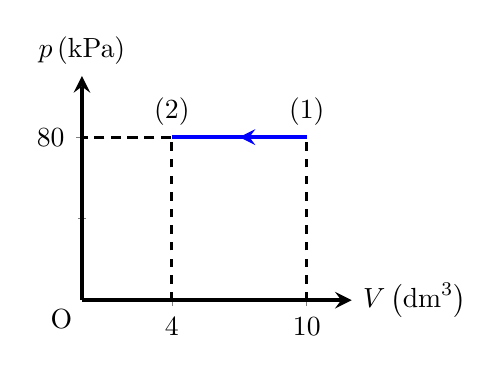
\begin{tikzpicture}  
			\begin{axis}[  ultra thick,scale=0.5,
				xmin=0,  
				xmax=12,  
				xtick={0,4,10},
				ytick={0,80},
				minor x tick num=1,
				minor y tick num=1,
				ymin=0,  
				ymax=110, 
				samples=300,
				axis lines=center, 
				xlabel=$\xsi{V}{\left(\si{\deci\meter^3}\right)}$, 		ylabel=$\xsi{p}{\left(\si{\kilo\pascal}\right)}$,
				every axis y label/.style={at=(current axis.above origin),anchor=south},  
				every axis x label/.style={at=(current axis.right of origin),anchor=west},  ]
				\coordinate (A) at (axis cs: 10,80);
				\coordinate (B) at (axis cs: 4,80);
				\coordinate (O) at (axis cs: 0,0);
				\draw[dashed, line width=1pt] (axis cs: 4,0)--(B)--(axis cs:0,80);
				\draw[dashed, line width=1pt] (axis cs: 10,0)--(A)--(axis cs:0,80);
				\draw[line width=1.5pt,blue,decoration={markings, mark=at position 0.5 with {\arrow{stealth}}},
				postaction={decorate}] (A)--(B);
				\node[above] at (A) {(1)};
				\node[above] at (B) {(2)};
			\end{axis}  
			\node[below left] at (O) {O};
		\end{tikzpicture}
	\end{center}
	\choiceTF[t]
	{Nhiệt độ của khối khí ở trạng thái (2) là $\SI{240}{\celsius}$}
	{\True Khối khí nhận một công có giá trị $\SI{480}{\joule}$}
	{Khối khí nhận từ môi trường bên ngoài một nhiệt lượng $\SI{1620}{\joule}$}
	{Nội năng của khối khí tăng thêm một lượng $\SI{1140}{\joule}$}
	\loigiai
	{
		\begin{itemchoice}
			\itemch Sai. Đẳng áp: $\dfrac{V_1}{T_1}=\dfrac{V_2}{T_2}\Rightarrow T_2=\SI{240}{\kelvin}$.
			\itemch Đúng. $A=-A'=p\left(V_1-V_2\right)=\SI{480}{\joule}$.
			\itemch Sai. Vì $T_2<T_1$ nên khối khí tỏa nhiệt.
			\itemch Sai. Vì $T_2<T_1$ nên nội năng khí giảm.
		\end{itemchoice}
	}
\end{ex}
\Closesolutionfile{ans}
\section{Câu trắc nghiệm trả lời ngắn} \textit{Thí sinh trả lời từ câu 1 đến câu 6}
\setcounter{ex}{0}
\Opensolutionfile{ans}[ans/G12-3-TL]
% ===============================================================
\begin{ex}
	Đồ thị biểu diễn sự phụ thuộc thể tích $V$ của một khối khí lí tưởng xác định theo nhiệt độ $t$ khi áp suất không đổi có dạng như hình vẽ. Nhiệt độ tại vị trí A bằng bao nhiêu $\si{\celsius}$? \textit{(Kết quả làm tròn đến phần nguyên)}.
	
	\begin{center}
		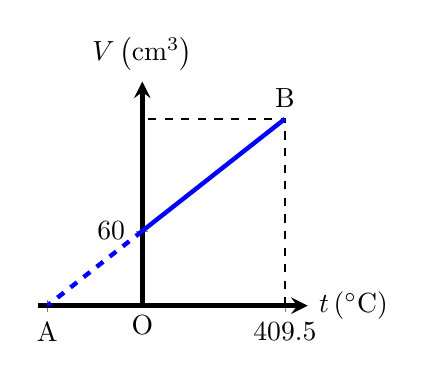
\begin{tikzpicture}  
			\begin{axis}[  ultra thick,scale=0.5,
				xmin=-300,  
				xmax=475,  
				xtick={-273,0,409.5},
				ytick={0,60},
				ymin=0,  
				xticklabels={A,0,409.5},
				ymax=180, 
				samples=300,
				axis lines=center, 
				xlabel=$\xsi{t}{\left(\si{\celsius}\right)}$, 		ylabel=$\xsi{V}{\left(\si{\centi\meter^3}\right)}$,
				every axis y label/.style={at=(current axis.above origin),anchor=south},  
				every axis x label/.style={at=(current axis.right of origin),anchor=west},  
				]
				\draw[dashed, line width=1pt] (axis cs: 409.5,0)--(axis cs: 409.5,150)--(axis cs: 0,150);
				\addplot [ultra thick, blue, smooth, domain=0:409.5] {60+20*x/91} ; 
				\addplot [ultra thick, blue, dashed,smooth, domain=0:-273] {60+20*x/91} ; 
				\node[above] at (409.5,150) {B};
				\coordinate (O) at (axis cs: 0,0);
			\end{axis}
			\node[below] at (O) {O};  
		\end{tikzpicture}
	\end{center}
	\shortans{ -273}
	\loigiai{
		Đẳng áp nên $\dfrac{V_{\mathrm{B}}}{T_{\mathrm{B}}}=\dfrac{V_{\mathrm{O}}}{T_{\mathrm{O}}}\Rightarrow V_{\mathrm{B}}=\SI{150}{\centi\meter^3}$.\\
		Ta có $V$ là hàm tuyến tính theo $t$ nên:
		$$\dfrac{t_{\mathrm{A}}-t_{\mathrm{O}}}{t_{\mathrm{B}}-t_{\mathrm{O}}}=\dfrac{V_{\mathrm{A}}-V_{\mathrm{O}}}{V_{\mathrm{B}}-V_{\mathrm{O}}}\Rightarrow t_{\mathrm{A}}=\SI{-273}{\celsius}.$$
	}
\end{ex}
% ===============================================================
\begin{ex}
	Biết nhiệt nóng chảy riêng của nước đá là $\SI{3.4E5}{\joule/\kilogram}$. Nhiệt lượng cần cung cấp để làm nóng chảy hoàn toàn $\SI{50}{\gram}$ nước đá ở $\SI{0}{\celsius}$ bằng bao nhiêu $\si{\kilo\joule}$? \textit{(Kết quả làm tròn đến phần nguyên)}.
	\shortans{ 17}
	\loigiai{
		$$Q=m\lambda=\SI{17}{\kilo\joule}.$$
	}
\end{ex}
% ===============================================================
\begin{ex}
	\immini{
		Một học sinh Trường TH - THCS - THPT Lê Thánh Tông làm thí nghiệm đun nóng chất X trên bếp điện và vẽ được đồ thị biểu diễn sự phụ thuộc nhiệt độ $\xsi{T}{(\celsius})$ của nó theo thời gian $\xsi{t}{(\minute)}$ như hình bên. Giá trị mỗi ô theo trục hoành là 5 phút, theo trục tung là $\SI{25}{\celsius}$. Trong quá trình thí nghiệm, chất X tan chảy và sau một thời gian nó sôi lên. Do vội vàng, học sinh này quên ghi nhiệt độ ban đầu của chất đó mà chỉ nhớ rằng trong 15 phút đầu công suất đốt nóng của bếp kém hơn 2 lần so với thời gian còn lại. Giả sử rằng năng lượng nhiệt tỏa ra từ bếp điện chỉ dùng để đun nóng chất X. Gọi nhiệt dung của chất X ở trạng thái rắn là $C_{1}$ và ở trạng thái lỏng là $C_{2}$. 
	}
	{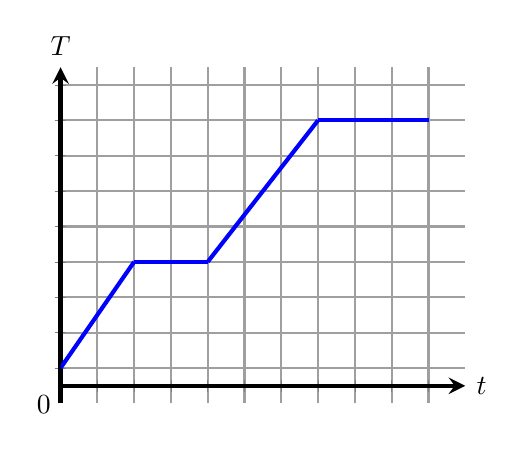
\begin{tikzpicture}  
			\begin{axis}[  ultra thick,scale=0.75,
				xmin=0,  
				xmax=11,  
				xtick={0,1,...,10},
				ytick={0,0.5,1.5, 2.5, 3.5,...,8.5},
				minor x tick num=0,
				minor y tick num=0,
				ymin=-0.5,  
				ymax=9, 
				samples=300,
				yticklabels=\empty,
				xticklabels=\empty,
				yticklabel style={/pgf/number format/.cd, fixed,
					fixed zerofill, precision=1}, %số chữ số thập phân
				axis lines=center, 
				grid style={step=1, line width =0.4pt, color=gray!40!white},
				grid=both, %giới hạn ô lưới
				major grid style={line width=0.8pt,gray!75!white},
				xlabel=$t$, 		ylabel=$T$,
				every axis y label/.style={at=(current axis.above origin),anchor=south},  
				every axis x label/.style={at=(current axis.right of origin),anchor=west},  ]
				\coordinate (O) at (0,0);
				\addplot [line width=1.5pt, blue, smooth, domain=0:2] {0.5+1.5*x};  
				\addplot [line width=1.5pt, blue, smooth, domain=2:4] {3.5};  
				\addplot [line width=1.5pt, blue, smooth, domain=4:7] {3.5+4*(x-4)/3};  
				\addplot [line width=1.5pt, blue, smooth, domain=7:10] {7.5};   
			\end{axis}  
			\node[below left]at (O) {0};
		\end{tikzpicture}
		
	}
	Tỉ số $C_{2} / C_{1}$ bằng bao nhiêu? \textit{(Kết quả lấy đến hai chữ số sau dấu phẩy thập phân)}.
	\shortans{2,25 }
	\loigiai{
		\begin{equation}
			\calP_1t_1=mC_1\Delta t_1\Leftrightarrow \calP_1\cdot 10=mC_1 \cdot25\cdot3
			\label{eq:1}
		\end{equation}
		\begin{equation}
			\calP_2t_2=mC_2\Delta t_2\Leftrightarrow 2\calP_1\cdot 15=mC_2 \cdot25\cdot4
			\label{eq:2}
		\end{equation}
		Từ \eqref{eq:1} và \eqref{eq:2}:
		$$\dfrac{C_2}{C_1}=\dfrac{30}{10}\cdot\dfrac{3}{4}=2,25.$$	}
\end{ex}
% ===============================================================
\begin{ex}
	\immini{
		Chuông lặn là một thiết bị chìm dưới nước để nghiên cứu các điều kiện trong nước, cũng có thể được sử dụng làm thiết bị lặn để sửa chữa các bộ phận dưới nước của trụ cầu và các công trình xây dựng khác. Một chuông lặn cao $\SI{2}{\meter}$ được thả chìm theo phương thẳng đứng từ mặt nước xuống đáy hồ nước sâu $\SI{10}{\meter}$ (hình vẽ). }	
	{
		\includegraphics[width=0.45\linewidth]{../figs/D12-2-8}
	}
	Giả sử nhiệt độ của khối khí (coi là khí lí tưởng) kèm theo trong chuông không đổi, áp suất khí quyển $p_{0}=\SI{E5}{\pascal}$, khối lượng riêng của nước là $\rho=\SI{E3}{\kilogram/\meter^3}$ và lấy $g=\SI{10}{\meter/\second^2}$. Độ cao $h$ của mực nước trong chuông bằng bao nhiêu mét? \textit{(Kết quả lấy đến hai chữ số sau dấu phẩy thập phân)}
	\shortans{0,95}
	\loigiai{
		\begin{center}
			\begin{tabular}{|M{5cm}|M{5cm}|M{5cm}|}
				\hline
				& $p$ &$V$\\
				\hline
				\thead{Ban đầu}&$p_0=\SI{E5}{\pascal}$ & $V_0=2S$\\
				\hline
				\thead{Lúc sau} & $p=p_0+\rho g\left(H-h\right)=10^5+10^4\cdot\left(10-h\right)$ & $V=\left(2-h\right)S$\\
				\hline
			\end{tabular}
		\end{center}
		Áp dụng định luật Boyle:
		$$p_0V_0=pV\Leftrightarrow 10^5\cdot2S=\left[10^5+10^4\cdot\left(10-h\right)\right]\cdot\left(2-h\right)S\Rightarrow h\approx\SI{0.95}{\meter}.$$
	}
\end{ex}
% ===============================================================
\begin{ex}
	\immini{
		Một khối khí lí tưởng thực hiện một chu trình biến đổi như hình vẽ. Cho $p$ là áp suất và $V$ là thể tích của khối khí. Biết $1-2$ là quá trình đẳng tích và $2-3$ là quá trình đẳng áp. Nhiệt độ của khối khí ở trạng thái 1 và 3 lần lượt là $T_{1}=\SI{320}{\kelvin}$ và $T_{3}=\SI{480}{\kelvin}$. Nhiệt độ của khối khí ở trạng thái 2 bằng bao nhiêu theo thang Kelvin $\left(\si{\kelvin}\right)$? \textit{(Kết quả làm tròn đến phần nguyên)}.
	}
	{
		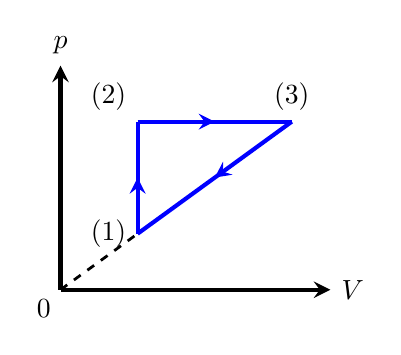
\begin{tikzpicture}  
			\begin{axis}[  ultra thick,scale=0.5,
				xmin=0,  
				xmax=7,  
				ymin=0,  
				ymax=8, 
				samples=300,
				xtick=\empty,
				ytick=\empty,
				yticklabels=\empty,
				xticklabels=\empty,
				axis lines=center, 
				xlabel=$V$, 		ylabel=$p$,
				every axis y label/.style={at=(current axis.above origin),anchor=south},  
				every axis x label/.style={at=(current axis.right of origin),anchor=west},  ]
				\coordinate (A) at (axis cs: 2,2);
				\coordinate (B) at (axis cs: 2,6);
				\coordinate (C) at (axis cs: 6,6);
				\coordinate (O) at (axis cs: 0,0);
				\draw[blue, line width=1.5pt, decoration={markings, mark=at position 0.5 with {\arrow{stealth}}},
				postaction={decorate}] (A)--(B);
				\draw[blue, line width=1.5pt, decoration={markings, mark=at position 0.5 with {\arrow{stealth}}},
				postaction={decorate}] (B)--(C);
				\draw[blue, line width=1.5pt, decoration={markings, mark=at position 0.5 with {\arrow{stealth}}},
				postaction={decorate}] (C)--(A);
				\draw[line width=1pt, dashed] (O)--(A);
				\node[left] at (A) {(1)};
				\node[above left] at (B) {(2)};
				\node[above] at (C) {(3)};
			\end{axis}  
			\node[below left] at(O) {0};
		\end{tikzpicture}
	}
	\shortans{392 }
	\loigiai{
		Ta có:
		$$\begin{cases}
			\dfrac{p_2}{p_1}=\dfrac{T_2}{T_1}\\
			\dfrac{V_3}{V_2}=\dfrac{T_3}{T_2}
		\end{cases}\ \text{hay} \ \begin{cases}
			\dfrac{p_3}{p_1}=\dfrac{T_2}{T_1}\\
			\dfrac{V_3}{V_1}=\dfrac{T_3}{T_2}
		\end{cases}$$
		Mà đường thẳng $(3)\rightarrow(1)$ đi qua gốc tọa độ nên:
		$$\dfrac{p_3}{p_1}=\dfrac{V_3}{V_1}\Rightarrow \dfrac{T_2}{T_1}=\dfrac{T_3}{T_2}\Rightarrow T_2=\sqrt{T_3T_1}\approx\SI{392}{\kelvin}.$$
	}
\end{ex}
% ===============================================================
\begin{ex}
	\immini{
		Một bạn học sinh đã thiết kế một thiết bị thí nghiệm để đo nhiệt độ môi trường bằng cân điện tử như hình bên. Xilanh dẫn nhiệt có đầu trên hở và được cố định trên bàn. Một pit-tông có khối lượng $m_{1}=\SI{600}{\gram}$ và diện tích mặt cắt ngang $S=\SI{20}{\centi\meter^2}$ được dùng để bịt kín một khối lượng khí lí tưởng nhất định trong xilanh. Bỏ qua ma sát giữa pit-tông và thành xilanh. 
	}
	{
		\includegraphics[width=0.55\linewidth]{../figs/D12-2-9}
	}
	Trọng tâm (điểm chính giữa) của một thanh nhẹ được đặt trên điểm tựa cố định A. Pit-tông được treo thẳng đứng ở đầu bên trái của thanh bằng một sợi dây nhẹ, không dãn. Một khối sắt có khối lượng $m_{2}=\SI{1200}{\gram}$ được treo thẳng đứng ở đầu bên phải bằng một sợi dây nhẹ, không dãn; khối sắt được đặt lên cân điện tử. Khi cân điện tử hiển thị giá trị ổn định 600 g thì nhiệt độ môi trường đo được là $\SI{27}{\celsius}$. 
	Cho áp suất khí quyển $p_{0}=\SI{E5}{\pascal}$ và lấy $g=\SI{10}{\meter/\second^2}$. Nhiệt độ lớn nhất mà thiết bị thí nghiệm này có thể đo được bằng bao nhiêu $\si{\celsius}$? \textit{(Kết quả làm tròn đến phần nguyên)}.
	\shortans{36 }
	\loigiai{
		Nếu nhiệt độ khí trong xilanh tăng, áp suất khí tăng, pit-tông bị đẩy đi lên $\Rightarrow$ dây bị chùn, thí nghiệm không còn đo được.\\
		\begin{center}
			\includegraphics[width=0.5\linewidth]{../figs/D12-2-10}
		\end{center}
		Vật nặng $m_2$ cân bằng:
		$$m_2g-F=mg\Rightarrow F=\left(m_2-m\right)g.$$
		Pit-tông cân bằng:
		$$pS+F=m_1g+p_0S\Rightarrow p=\dfrac{m_1g+p_0S-F}{S}=\dfrac{\left(m_1+m-m_2\right)g+p_0S}{S}.$$
		Tại nhiệt độ $T_1=\SI{300}{\kelvin}$ thì số chỉ của cân là $m=\SI{600}{\gram}$, khi đó áp suất khí trong xilanh là:
		$$p_1=p_0=\SI{E5}{\pascal}.$$
		Thí nghiệm sẽ không còn đo được khi dây chùn $\left(F=0\right)$, khi đó:
		$$p_2=\dfrac{m_1g+p_0S}{S}=\SI{1.03E5}{\pascal}.$$
		Trong quá trình thí nghiệm, dây không chùn nên thể tích khí trong xilanh không đổi:
		$$\dfrac{p_2}{T_2}=\dfrac{p_1}{T_1}\Rightarrow T_2=\SI{309}{\kelvin}\Rightarrow t_2=\SI{36}{\celsius}.$$
	}
\end{ex}
\Closesolutionfile{ans}
\begin{center}
	\textbf{-- HẾT --}
\end{center}
%\chapter{Đề 4}
%\begin{tabular}{M{6.5cm}M{11cm}}
	\textbf{LỚP CÔ THẢO - THẦY SANG}& \textbf{ĐỀ ÔN TẬP KIỂM TRA GIỮA HỌC KÌ 1}\\
	\textbf{MÃ ĐỀ: 004}& \textbf{Bài thi môn: VẬT LÝ 12}\\
	\textit{(Đề trường Nguyễn Khuyến TpHCM\newline năm học 2024 -2025)}& \textit{Thời gian làm bài: 50 phút, không kể thời gian phát đề}
	
	\noindent\rule{4cm}{0.8pt} \\
\end{tabular}
\setcounter{section}{0}
\begin{center}
	\textbf{\large BẢNG ĐÁP ÁN}
\end{center}
\section{}
\inputansbox{10}{ans/G12-4-TN}
\section{}
\inputansbox[2]{2}{ans/G12-4-TF}
\section{}
\inputansbox[3]{6}{ans/G12-4-TL}\newpage
%\begin{tabular}{M{6.5cm}M{11cm}}
	\textbf{LỚP CÔ THẢO - THẦY SANG}& \textbf{ĐỀ ÔN TẬP KIỂM TRA GIỮA HỌC KÌ 1}\\
	\textbf{MÃ ĐỀ: 004}& \textbf{Bài thi môn: VẬT LÝ 12}\\
	\textit{(Đề trường Nguyễn Khuyến TpHCM\newline năm học 2024 -2025)}& \textit{Thời gian làm bài: 50 phút, không kể thời gian phát đề}
	
	\noindent\rule{4cm}{0.8pt} \\
\end{tabular}
\setcounter{section}{0}
\section{Câu trắc nghiệm nhiều phương án lựa chọn}
\textit{Thí sinh trả lời từ câu 1 đến câu 18. Mỗi câu hỏi thí sinh chọn một phương án}
\setcounter{ex}{0}
\Opensolutionfile{ans}[ans/G12-4-TN]
% ===================================================================
\begin{ex}
	Nhiệt dung riêng của một chất là nhiệt lượng cần thiết để làm cho
	\choice
	{$\SI{1}{\meter^3}$ chất đó tăng thêm $\SI{1}{\celsius}$}
	{$\SI{1}{\kilogram}$ chất đó tăng thêm $\SI{100}{\celsius}$}
	{\True $\SI{1}{\kilogram}$ chất đó tăng thêm $\SI{1}{\celsius}$}
	{$\SI{1}{\meter^3}$ chất đó tan chảy hoàn toàn}
	\loigiai{}
\end{ex}
% ===================================================================
\begin{ex}
Cách làm thay đổi nội năng chủ yếu bằng hình thức thực hiện công cơ học là	
	\choice
	{bỏ miếng kim loại vào nước đá}
	{bỏ miếng kim loại vào nước nóng}
	{hơ nóng miếng kim loại trên ngọn lửa đèn cồn}
	{\True ma sát (chà) một miếng kim loại trên mặt bàn}
	\loigiai{}
\end{ex}
% ===================================================================
\begin{ex}
	Chuyển động của các phân tử, nguyên tử được gọi là
	\choice
	{dao động cơ}
	{dao động điều hòa}
	{\True chuyển động nhiệt}
	{chuyển động từ}
	\loigiai{}
\end{ex}
% ===================================================================
\begin{ex}
	Nhiệt độ âm trong thang nhiệt độ Celsius là nhiệt độ
	\choice
	{tan chảy của nước đá}
	{\True thấp hơn $\SI{0}{\celsius}$}
	{từ $\SI{35}{\celsius}$ đến $\SI{42}{\celsius}$}
	{từ $\SI{0}{\celsius}$ đến $\SI{100}{\celsius}$}
	\loigiai{}
\end{ex}
% ===================================================================
\begin{ex}
	Gọi $m$ là khối lượng của một phân tử của một chất khí. Biết khối khí này có $N$ phân tử, thể tích là $V$. Khối lượng riêng của chất khí này là
	\choice
	{$\dfrac{V}{Nm}$}
	{\True $\dfrac{Nm}{V}$}
	{$\dfrac{m}{NV}$}
	{$\dfrac{m}{V}$}
	\loigiai{}
\end{ex}
% ===================================================================
\begin{ex}
Một số chất ở thể rắn như iodine, băng phiến, đá khô,\dots có thể chuyển trực tiếp sang \dots (1) 
\dots khi nó \dots (2) \dots Hiện tượng trên gọi là sự thăng hoa. Ngược lại với sự thăng hoa là sự ngưng kết. Điền cụm từ thích hợp vào chố trống.	
	\choice
	{(1) thể lỏng; (2) nhận nhiệt}
	{\True (1) thể hơi; (2) nhận nhiệt}
	{(1) thể lỏng; (2) tỏa nhiệt}
	{(1) thể hơi; (2) tỏa nhiệt}
	\loigiai{}
\end{ex} %===================================================================
%
\begin{ex}
	Trong hệ SI, đơn vị của nhiệt nóng chảy riêng là
	\choice
	{\True $\si{\joule/\kilogram}$}
	{$\si{cal}$}
	{$\si{\electronvolt}$}
	{$\si{\joule}$}
	\loigiai{}
\end{ex}
% ===================================================================
\begin{ex}
	Điều nào sau đây là \textbf{sai} khi nói về nội năng?
	\choice
	{\True Nội năng không thể biến đổi được}
	{Nội năng của một vật phụ thuộc vào nhiệt độ và thể tích của vật}
	{Đơn vị của nội năng là Jun ($\si{\joule}$)}
	{Nội năng của một vật là dạng năng lượng bao gồm tổng động năng của các phân tử cấu tạo nên vật và thế năng tương tác giữa chúng}
	\loigiai{}
\end{ex}
% ===================================================================
\begin{ex}
Hai vật rắn (1) và (2) tiếp xúc nhau. Vật (1) đang có nhiệt độ cao hơn vật (2). Phát biểu nào sau đây \textbf{không} chính xác?	
	\choice
	{\True Vật (1) có nội năng lớn hơn vật (2)}
	{Năng lượng nhiệt được truyền từ vật (1) sang vật (2)}
	{Tốc độ trung bình của các phân tử trong vật (1) cao hơn tốc độ trung bình của các phân tử trong vật (2)}
	{Quá trình truyền nhiệt giữa 2 vật dừng lại khi chúng có nhiệt độ bằng nhau}
	\loigiai{
	Nội năng của 1 hệ phụ thuộc nhiệt độ và thể tích của hệ, nhiệt độ hệ (1) cao hơn hệ (2) chưa chắc nội năng hệ (1) lớn hơn nội năng hệ (2).
	}
\end{ex}
% ===================================================================
\begin{ex}
	Tính chất nào sau đây \textbf{không phải} của nguyên tử, phân tử?
	\choice
	{\True Nở ra khi nhiệt độ tăng, co lại khi nhiệt độ giảm}
	{Chuyển động càng nhanh khi nhiệt độ càng cao}
	{Giữa chúng có khoảng cách}
	{Chuyển động không ngừng}
	\loigiai{}
\end{ex}
% ===================================================================
\begin{ex}
Trong các chất sau, chất nào không phải là chất rắn kết tinh?	
	\choice
	{Nước đá}
	{Muối ăn}
	{Kim cương}
	{\True Nhựa đường}
	\loigiai{}
\end{ex}
% ===================================================================
\begin{ex}
	Tính chất nào sau đây \textbf{không phải} là tính chất của chất ở thể khí?
	\choice
	{Có thể nén được dễ dàng}
	{\True Có hình dạng và thể tích riêng}
	{Có các phân tử chuyển động hỗn độn}
	{Có lực tương tác phân tử nhỏ hơn lực tương tác phân tử ở thể rắn và thể lỏng}
	\loigiai{}
\end{ex}
% ===================================================================
\begin{ex}
	Bảng dưới đây cho biết nhiệt độ nóng chảy và nhiệt độ sôi của một số chất
	\begin{center}
		\begin{tabular}{|M{5cm}|M{5cm}|M{5cm}|}
		\hline
		\thead{Chất}&\thead{Nhiệt độ nóng chảy $\left(\si{\celsius}\right)$} &\thead{Nhiệt độ sôi $\left(\si{\celsius}\right)$}\\
		\hline
		1&$\SI{-201}{}$&$\SI{-196}{}$\\
		\hline
		2&$\SI{-39}{}$&357\\
		\hline
		3&30&2400\\
		\hline
		4&327&1749\\
		\hline
		\end{tabular}
	\end{center}
	Chất nào ở thể lỏng ở $\SI{20}{\celsius}$?
	\choice
	{\True Chất 2}
	{Chất 1}
	{Chất 3}
	{Chất 4}
	\loigiai{}
\end{ex}
% ===================================================================
\begin{ex}
	Hình dưới đây biểu diễn sự thay đổi nhiệt độ theo thời gian của chất A
	\begin{center}
		\includegraphics[width=0.7\linewidth]{../figs/D12-4-1}
	\end{center}
	Nhận xét nào sau đây \textbf{không đúng}?
	\choice
	{Nhiệt độ sôi của chất A là $\SI{120}{\celsius}$}
	{\True Ở phút thứ 8 , chất A tồn tại ở cả 3 thể rắn, lỏng và khí (hơi)}
	{Nhiệt độ nóng chảy của chất A là $\SI{40}{\celsius}$}
	{Ở phút thứ 4 , chất A đang ngưng tụ}
	\loigiai{
	Ở phút thứ 8 chất này chỉ tồn tại ở thể lỏng.
	}
\end{ex}
% ===================================================================
\begin{ex}
	Ở nhiệt độ bao nhiêu trong thang Celsius thì giá trị nhiệt độ bằng một nửa nhiệt độ tuyệt đối của nó?
	\choice
	{$\SI{50}{\celsius}$}
	{$\SI{0}{\celsius}$}
	{$\SI{100}{\celsius}$}
	{\True $\SI{273}{\celsius}$}
	\loigiai{
	$$t=\dfrac{t+273}{2}\Rightarrow t=\SI{273}{\celsius}.$$
	}
\end{ex}
% ===================================================================
\begin{ex}
	Một khối khí dãn nở thêm 1 lít ở áp suất không đổi là $\SI{E5}{\newton/\meter^2}$. Trong quá trình này, khối khí nhận thêm nhiệt lượng là $\SI{500}{\joule}$. Độ biến thiên nội năng của khí là
	\choice
	{$\SI{600}{\joule}$}
	{$\SI{-600}{\joule}$}
{\True $\SI{400}{\joule}$}
	{$\SI{-400}{\joule}$}
	\loigiai{
	Công khối khí thực hiện:
	$$A'=p\Delta V=\left(\SI{E5}{\newton/\meter^2}\right)\cdot\left(\SI{1E-3}{\meter^3}\right)=\SI{100}{\joule}.$$
	Độ biến thiên nội năng của khí:
	$$\Delta U=Q+A=Q-A'=\SI{400}{\joule}.$$
	}
\end{ex}
% ===================================================================
\begin{ex}
	Nhiệt lượng cần cung cấp để một khối băng có khối lượng $\SI{2}{\kilogram}$ tan chảy hoàn toàn ở nhiệt độ tan chảy $\SI{0}{\celsius}$ là $\SI{666}{\kilo\joule}$. Nhiệt nóng chảy riêng của băng bằng
	\choice
	{$\SI{68}{\kilo\joule/\kilogram}$}
	{\True $\SI{333}{\kilo\joule/\kilogram}$}
	{$\SI{136}{\kilo\joule/\kilogram}$}
	{$\SI{170}{\kilo\joule/\kilogram}$}
	\loigiai{
	$$\lambda=\dfrac{Q}{m}=\SI{333}{\kilo\joule/\kilogram}.$$
	}
\end{ex}
% ===================================================================
\begin{ex}
	Biết nhiệt hóa hơi riêng của nước ở $\SI{100}{\celsius}$ là $\SI{2.26E6}{\joule/\kilogram}$. Nhiệt lượng cần thiết để chuyển $\SI{2.5}{\kilogram}$ nước ở $\SI{100}{\celsius}$ thành hơi hoàn toàn là
	\choice
	{\True $\SI{5650}{\kilo\joule}$}
	{$\SI{904}{\kilo\joule}$}
	{$\SI{904}{\joule}$}
	{$\SI{5650}{\joule}$}
	\loigiai{
	$$Q=mL=\left(\SI{2.5}{\kilogram}\right)\cdot\left(\SI{2.26E6}{\joule/\kilogram}\right)=\SI{5650}{\kilo\joule}.$$
	}
\end{ex}
\Closesolutionfile{ans}
\section{Câu trắc nghiệm đúng/sai} 
\textit{Thí sinh trả lời từ câu 1 đến câu 4. Trong mỗi ý \textbf{a)}, \textbf{b)}, \textbf{c)}, \textbf{d)} ở mỗi câu, thí sinh chọn đúng hoặc sai}
\setcounter{ex}{0}
\Opensolutionfile{ans}[ans/G12-4-TF]
% ===================================================================
\begin{ex}
	\immini{
	Một lượng khí chứa trong một xilanh có pittông di chuyển được. Ở trạng thái cân bằng, chất khí chiếm thể tích $V\left(\si{\meter^3}\right)$ và tác dụng lên pittông một áp suất $\SI{4E5}{\newton/\meter^2}$. Khối khí nhận một nhiệt lượng $\SI{1000}{\joule}$ giãn nở đẩy pittông lên làm thể tích khí tăng thêm $\SI{0.003}{\meter^3}$. Coi rằng áp suất chất khí không đổi.
	}
	{
	\includegraphics[width=0.4\linewidth]{../figs/D12-4-2}
	}
	\choiceTF[t]
	{Theo quy ước, khối khí nhận nhiệt và sinh công nên $A>0$; $A>0$}
	{\True Độ biến thiên nội năng của khối khí $\Delta U=\SI{-200}{\joule}$}
	{\True Công mà khối khí thực hiện có độ lớn bằng $\SI{1200}{\joule}$}
	{\True Lượng khí bên trong xilanh nhận nhiệt và sinh công làm biến đổi nội năng}
	\loigiai{
	\begin{itemchoice}
		\itemch Sai. $Q>0$, $A<0$.
		\itemch Đúng. $\Delta U=Q-A'=Q-p\Delta V=\SI{-200}{\joule}$.
		\itemch Đúng. $A'=p\Delta V=\SI{1200}{\joule}$.
		\itemch Đúng.
	\end{itemchoice}
	}
\end{ex}
% ===================================================================
\begin{ex}
	Một lượng khí chứa trong một bình thép kín được nung nóng. Bỏ qua sự thay đổi thể tích của bình chứa.
	\choiceTF[t]
	{\True Nếu mỗi phân tử khí có khối lượng $\SI{3.3E-26}{\kilogram}$; bình có thể tích $\SI{20}{\centi\meter^3}$ và số phân tử khí trong bình là $10^{21}$ thì khối lượng riêng của chất khí là $\SI{16.5E-6}{\kilogram/\centi\meter^3}$}
	{Khối lượng riêng của chất khí trong bình tăng lên}
	{Mật độ phân tử khí trong bình tăng lên}
	{\True Tốc độ chuyển động trung bình của các phân tử khí tăng lên}
	\loigiai{
	\begin{itemchoice}
		\itemch Đúng. $D=\dfrac{Nm}{V}=\SI{1.65E-6}{\kilogram/\centi\meter^3}$.
		\itemch Sai.  $N, m, V$ không đổi nên $D$ không đổi.
		\itemch Sai. $N, V$ không đổi nên mật độ phân tử khí $\mu=\dfrac{N}{V}$ không đổi.
		\itemch Đúng. Nhiệt độ tăng nên tốc độ chuyển động nhiệt của các phân tử khí tăng.
	\end{itemchoice}
	}
\end{ex}
% ===================================================================
\begin{ex}
	 Hai vật rắn A và B được làm bằng hai kim loại khác nhau nhưng có cùng khối lượng và được nung nóng đều đặn trong các điều kiện giống nhau. Nhiệt độ của mỗi vật theo thời gian được mô tả bởi đồ thị ở hình bên.
	 \begin{center}
	 	\begin{tikzpicture}  
	 		\begin{axis}[  ultra thick,yscale=0.75,
	 			xmin=0,  
	 			xmax=9,  
	 			xtick={0,1,...,8},
	 			ytick={0,30,...,150},
	 			minor x tick num=0,
	 			minor y tick num=0,
	 			ymin=0,  
	 			ymax=170, 
	 			samples=300,
	 			axis lines=center, 
	 			grid style={step=1, line width =0.6pt, color=gray!50!white},
	 			grid=both, %giới hạn ô lưới
	 			major grid style={line width=0.8pt,gray!85!white},
	 			xlabel=$\xsi{t}{\left(\si{\second}\right)}$, 		ylabel=$\text{Nhiệt độ}\ \si{\celsius}$,
	 			every axis y label/.style={at=(current axis.above origin),anchor=south},  
	 			every axis x label/.style={at=(current axis.right of origin),anchor=west},  ]
	 			\addplot [line width=2pt, red, smooth, domain=0:3] {40*x} node[above left] {A};  
	 			\addplot [line width=2pt, blue, smooth, domain=0:6] {15*x} node[above left] {B}; 
	 			\coordinate (O) at (0,0);
	 		\end{axis}  
	 		\node[below left] at (O) {O};
	 	\end{tikzpicture}
	 \end{center}
	\choiceTF[t]
	{\True Tốc độ tăng nhiệt độ của vật A nhanh hơn tốc độ tăng nhiệt độ của vật B}
	{Ở giây thứ 2 , nhiệt độ của vật A bằng $\SI{78}{\celsius}$}
	{\True Ở giây thứ 2 nhiệt độ của vật B bằng $\SI{30}{\celsius}$}
	{\True Tỉ số nhiệt dung riêng của kim loại A so với nhiệt dung riêng của kim loại B là 0,375}
	\loigiai{
	\begin{itemchoice}
		\itemch Đúng.
		\itemch Sai. $t=\dfrac{2}{3}t_A=\dfrac{2}{3}\cdot120=\SI{80}{\celsius}$.
		\itemch Đúng. 
		\itemch Sai. $\calP=\dfrac{mc_A\cdot120}{3}=\dfrac{mc_B\cdot90}{6}\Rightarrow \dfrac{c_A}{c_B}=0,375.$
	\end{itemchoice}
	}
\end{ex}
% ===================================================================
\begin{ex}
	Một khối nước đá tinh khiết có khối lượng $m=\SI{800}{\gram}$ ở $\SI{-10}{\celsius}$. Biết nhiệt dung riêng của nước đá là $c_{1}=\SI{2090}{\joule/\kilogram\cdot\kelvin}$; nhiệt nóng chảy riêng của nước đá $\lambda=\SI{3.33E5}{\joule/\kilogram}$.
	\choiceTF[t]
	{Khi nước đá tan chảy nó tỏa nhiệt lượng ra môi trường}
	{\True Nhiệt lượng cần thiết để làm cho khối nước đá tăng từ  $\SI{-10}{\celsius}$ lên đến $\SI{0}{\celsius}$ bằng $\SI{16720}{\joule}$}
	{\True Để khối nước đá ở trạng thái trên nóng chảy hoàn toàn thành thể lỏng thì cần một nhiệt lượng tối thiểu là $\SI{283.12}{\kilo\joule}$}
	{\True Ở điều kiện tiêu chuẩn, nước đá tinh khiết nóng chảy ở $\SI{0}{\celsius}$}
	\loigiai{
	
	}
\end{ex}
\Closesolutionfile{ans}
\section{Câu trắc nghiệm trả lời ngắn} \textit{Thí sinh trả lời từ câu 1 đến câu 6}
\setcounter{ex}{0}
\Opensolutionfile{ans}[ans/G12-4-TL]
% ===============================================================
\begin{ex}
	Biết nhiệt nóng chảy riêng của nước đá là $\lambda=\SI{34E4}{\joule/\kilogram}$ và nhiệt dung riêng của nước là $\SI{4180}{\joule/\kilogram\cdot\kelvin}$. Nhiệt lượng cần cung cấp cho $\SI{4}{\kilogram}$ nước đá ở $\SI{0}{\celsius}$ để chuyển nó thành nước $\SI{20}{\celsius}$ là bao nhiêu $\si{\kilo\joule}$? \textit{(Làm tròn đến phần nguyên của kết quả)}
	\shortans{1694}
	\loigiai{
		$$Q=m\left(\lambda+ct\right)=\SI{1694400}{\joule}\approx\SI{1694}{\kilo\joule}.$$
	}
\end{ex}
% ===============================================================
\begin{ex}
	Biết nhiệt dung riêng của nước đá là $c_{1}=\SI{2100}{\joule/\kilogram\cdot\kelvin}$, nhiệt dung riêng của nước là $c_{2}=\SI{4200}{\joule/\kilogram\cdot\kelvin}$. Để tìm nhiệt nóng chảy riêng của nước đá, người ta làm thí nghiệm như sau: Dùng một bếp điện để đun một hệ gồm một bình bằng đồng đựng một lượng nước đá với nhiệt độ ban đầu của hệ là $\SI{-5}{\celsius}$. Dùng nhiệt kế để đo nhiệt độ của hệ, người ta thu được bảng sau:
	\begin{center}
		\begin{tabular}{|M{3cm}|M{1.5cm}|M{1.5cm}|M{1.5cm}|M{1.5cm}|M{1.5cm}|M{1.5cm}|M{1.5cm}|M{1.5cm}|}
		\hline
		\thead{Thời gian $\left(\si{\second}\right)$} & 0& 60 & 360 & 660 & 960 & 1260 &1340 & 1540\\
		\hline
		\thead{Nhiệt độ $\left(\si{\celsius}\right)$}& $\SI{-5}{}$ & 0&0&0&0&0&0&10\\
		\hline
		\end{tabular}
	\end{center}
	Biết rằng từ thời điểm 0 đến $\SI{60}{\second}$ và $\SI{1340}{\second}$ đến $\SI{1540}{\second}$, số chỉ của nhiệt kế tăng liên tục. Coi như nhiệt lượng mà hệ nhận được tỉ lệ với thời gian đun (hệ số tỉ lệ không đổi). Nhiệt nóng chảy riêng của nước đá đo được trong thí nghiệm này là $\xsi{x\cdot10^5}{\joule/\kilogram}$. Giá trị của $x$ bằng bao nhiêu?
	\shortans{3,36 }
	\loigiai{
		Gọi $m$ và $m_b$ lần lượt là khối lượng của nước đá và khối lượng của bình.\\
		$$\begin{cases}
			\calP\cdot60=\left(mc_1+m_bc_b\right)\cdot 5\\
			\calP\cdot\left(1340-60\right)=m\lambda\\
			\calP\cdot\left(1540-1340\right)=\left(mc_2+m_bc_b\right)\cdot10
		\end{cases}\Rightarrow \begin{cases}
		\dfrac{m}{\calP}\cdot2100+\dfrac{m_bc_b}{\calP}=\dfrac{60}{5}\\
		\dfrac{m\lambda}{\calP}=1340-60\\
		\dfrac{m}{\calP}\cdot4200+\dfrac{m_bc_b}{\calP}=\dfrac{1540-1340}{10}
		\end{cases}\Rightarrow\begin{cases}
		\dfrac{m}{\calP}=\dfrac{2}{525}\\
		\lambda=\SI{3.36E5}{\joule/\kilogram}\\
		\dfrac{m_bc_b}{\calP}=4
		\end{cases}.$$
	}
\end{ex}
% ===============================================================
\begin{ex}
	Trong một bình nhiệt lượng kế có chứa $\SI{200}{\milli\liter}$ nước ở nhiệt độ ban đầu $t_{0}=\SI{10}{\celsius}$. Người ta dùng một cốc đổ $\SI{50}{\milli\liter}$ nước ở nhiệt độ $\SI{60}{\celsius}$ vào bình rồi sau khi cân bằng nhiệt lại múc ra từ bình $\SI{50}{\milli\liter}$ nước. Bỏ qua sự trao đổi nhiệt với cốc bình và môi trường. Hỏi sau tối thiểu bao nhiêu lượt đổ thì nhiệt độ của nước trong bình sẽ lớn hơn $\SI{40}{\celsius}$? 
	\textit{(Một lượt đổ gồm một lần múc nước vào và một lần múc nước ra).}
	\shortans{5}
	\loigiai{
		Sau $n$ lượt đổ thì nhiệt độ cân bằng là
		$$t_n=\dfrac{m_0t_{n-1}+t\Delta m}{m_0+\Delta m}=\dfrac{200t_{n-1}+50\cdot60}{200+50}.$$
		Chạy vòng lặp:
		$$A=A+1:X=\dfrac{200X+3000}{250}$$
		Với $A$ là số lượt đổ, giá trị đầu $A=0; X=10$. Tới $A=5$ thu được $X=\SI{43.616}{\celsius}$
	}
\end{ex}
% ===============================================================
\begin{ex}
	\immini{
	Trong một hệ đun nước bằng năng lượng Mặt Trời, năng lượng Mặt Trời thu thập từ những mặt ngoài của phần góp, nó làm cho nước lưu thông qua các ống của phần góp. Bức xạ Mặt Trời đi vào trong phần góp qua các lớp phủ trong suốt, làm nóng nước trong ống. Nước này được bơm vào các bình chứa. Giả thiết rằng hiệu suất của toàn bộ hệ là $\SI{20}{\percent}$ (nghĩa là $\SI{80}{\percent}$ năng lượng Mặt Trời bị mất khỏi hệ).}
	{
	\includegraphics[width=0.6\linewidth]{../figs/D12-4-3}
	}
	Hỏi diện tích của phần góp là bao nhiêu mét vuông khi cần nâng nhiệt độ của 200 lít nước trong bình chứa từ $\SI{20}{\celsius}$ đến $\SI{40}{\celsius}$ trong 1 giờ. Biết khối lượng riêng của nước là $\SI{1000}{\kilogram/\meter^3}$; nhiệt dung riêng của nước là $\SI{4190}{\joule/\kilogram\cdot\kelvin}$; cường độ của ánh sáng Mặt Trời tới là $\SI{700}{\watt/\meter^2}$. \textit{(Kết quả lấy đến một chữ số sau dấu phẩy thập phân)}
	\shortans{33,3 }
	\loigiai{
		Nhiệt lượng cần thiết để làm nóng nước:
	$$Q=mc\Delta t=DVc\Delta t=\SI{16.76E6}{\joule}$$
	Năng lượng cần nhận từ Mặt Trời:
	$$W=\dfrac{Q}{H}=	\SI{83.8E6}{\joule}.$$
	Diện tích phần góp:
	$$\dfrac{W}{t}=IS\Rightarrow S\approx\SI{33.3}{\meter^2}.$$
	
	}
\end{ex}
% ===============================================================
\begin{ex}
	Đầu thép của một búa máy có khối lượng $\SI{10}{\kilogram}$ nóng lên thêm $\SI{20}{\celsius}$ sau 2 phút hoạt động. Biết rằng chỉ có $\SI{50}{\percent}$ cơ năng của búa máy chuyển thành nhiệt năng của đầu búa. Lấy nhiệt dung riêng của thép là $\SI{460}{\joule/\kilogram\cdot\kelvin}$. Công suất của búa bằng bao nhiêu $\si{\kilo\watt}$? \textit{(Kết quả lấy đến một chữ số sau dấu phẩy thập phân)}.
	\shortans{1,5 }
	\loigiai{
	Nhiệt lượng làm nóng đầu búa máy:
	$$Q=mc\Delta t=\SI{92000}{\joule}.$$
	Công suất búa máy:
	$$\calP=\dfrac{Q}{Ht}\approx\SI{1.5}{\kilo\watt}.$$
	}
\end{ex}
% ===============================================================
\begin{ex}
	Một ấm nước bằng kim loại có khối lượng $\SI{300}{\gram}$ và chứa 2 lít nước. Khi nhận được nhiệt lượng $\SI{517.44}{\kilo\joule}$, nhiệt độ của ấm và nước tăng từ $\SI{20}{\celsius}$ lên $\SI{80}{\celsius}$. Biết nhiệt dung riêng của nước là $\SI{4180}{\joule/\kilogram\cdot\kelvin}$, khối lượng riêng của nước là $\SI{1000}{\kilogram/\meter^3}$. Nhiệt dung riêng của kim loại làm ấm bằng bao nhiêu $\si{\joule/\kilogram\cdot\kelvin}$?
	\shortans{880 }
	\loigiai{
		$$Q=\left(m_nc_n+m_ac_a\right)\Delta t\Rightarrow c_a=\SI{880}{\joule/\kilogram\cdot\kelvin}.$$
	}
\end{ex}

\Closesolutionfile{ans}
\begin{center}
	\textbf{-- HẾT --}
\end{center}
%\chapter{Đề 5}
%\begin{tabular}{M{6.5cm}M{11cm}}
	\textbf{LỚP CÔ THẢO - THẦY SANG}& \textbf{ĐỀ ÔN TẬP KIỂM TRA CUỐI HỌC KÌ 1}\\
	\textbf{MÃ ĐỀ: 005}& \textbf{Bài thi môn: VẬT LÝ 12}\\
	\textit{(Đề thi có 05 trang)}& \textit{Thời gian làm bài: 50 phút, không kể thời gian phát đề}
	
	\noindent\rule{4cm}{0.8pt} \\
\end{tabular}
\setcounter{section}{0}
\begin{center}
	\textbf{\large BẢNG ĐÁP ÁN}
\end{center}
\section{}
\inputansbox{10}{ans/G12-5-TN}
\section{}
\inputansbox[2]{2}{ans/G12-5-TF}
\section{}
\inputansbox[3]{6}{ans/G12-5-TL}\newpage
\begin{tabular}{M{6.5cm}M{11cm}}
	\textbf{TRUNG TÂM MANABIE}& \textbf{ĐỀ ÔN TẬP KIỂM TRA GIỮA HỌC KÌ 1}\\
	\textbf{MÃ ĐỀ: 005}& \textbf{Bài thi môn: VẬT LÝ 12}\\
	\textit{(Đề thi có 05 trang)}& \textit{Thời gian làm bài: 50 phút, không kể thời gian phát đề}
	
	\noindent\rule{4cm}{0.8pt} \\
\end{tabular}
\setcounter{section}{0}
\section{Câu trắc nghiệm nhiều phương án lựa chọn}
\textit{Thí sinh trả lời từ câu 1 đến câu 18. Mỗi câu hỏi thí sinh chọn một phương án}
\setcounter{ex}{0}
\Opensolutionfile{ans}[ans/G12-5-TN]
% ===================================================================
\begin{ex}
Đặc điểm nào sau đây là của sự bay hơi?	
	\choice
	{Chỉ xảy ra đối với một số ít chất lỏng}
	{Xảy ra với tốc độ như nhau ở mọi nhiệt độ}
	{\True Xảy ra ở bất kì nhiệt độ nào của chất lỏng}
	{Chỉ xảy ra trong lòng chất lỏng}
	\loigiai{}
\end{ex}
% ===================================================================
\begin{ex}
	Tính chất nào sau đây \textbf{không phải} của phân tử vật chất ở thể khí
	\choice
	{Chuyển động không ngừng}
	{\True Chuyển động hỗn loạn xung quanh các vị trí cân bằng cố định}
	{Nhiệt độ càng cao các phân tử chuyển động càng nhanh}
	{Chuyển động hỗn loạn}
	\loigiai{}
\end{ex}
% ===================================================================
\begin{ex}
Nhiệt độ không tuyệt đối $\left(\SI{0}{\kelvin}\right)$ là nhiệt độ mà tại đó các phân tử có	
	\choice
	{động năng chuyển động nhiệt bằng không và thế năng tương tác giữa chúng là cực đại}
	{động năng chuyển động nhiệt cực đại và thế năng tương tác giữa chúng là cực đại}
	{\True động năng chuyển động nhiệt bằng không và thế năng tương tác giữa chúng là tối thiểu}
	{động năng chuyển động nhiệt cực đại và thế năng tương tác giữa chúng là bằng không}
	\loigiai{}
\end{ex}
% ===================================================================
\begin{ex}
	Nếu hai vật có nhiệt độ khác nhau được đặt tiếp xúc nhau thì
	\choice
	{quá trình truyền nhiệt dừng lại khi nhiệt độ một vật đạt $\SI{0}{\celsius}$}
	{quá trình truyền nhiệt dừng lại khi nhiệt năng hai vật bằng nhau}
	{\True quá trình truyền nhiệt dừng lại khi nhiệt độ hai vật bằng nhau}
	{quá trình truyền nhiệt dừng lại khi độ biến thiên nhiệt độ hai vật bằng nhau}
	\loigiai{}
\end{ex}
% ===================================================================
\begin{ex}
Trạng thái của một lượng khí lí tưởng xác định được xác định bởi	
	\choice
	{áp suất, thể tích và khối lượng}
	{\True áp suất, nhiệt độ và thể tích}
	{khối lượng mol, áp suất và nhiệt độ}
	{thể tích, nhiệt độ và số mol}
	\loigiai{}
\end{ex}
% ===================================================================
\begin{ex}
	Nhiệt độ cơ thể người là $\SI{37}{\celsius}$ sẽ tương ứng với nhiệt độ bao nhiêu trong thang đo nhiệt độ Kelvin?
	\choice
	{\True $\SI{310}{\kelvin}$}
	{$\SI{300}{\kelvin}$}
	{$\SI{236}{\kelvin}$}
	{$\SI{210}{\kelvin}$}
	\loigiai{}
\end{ex}
% ===================================================================
\begin{ex}
	Khi các nguyên tử, phân tử cấu tạo nên vật chuyển động nhanh lên thì đại lượng nào sau đây tăng lên?
	\choice
	{Thế năng của vật tăng lên}
	{Khối lượng của vật}
	{Động năng của vật tăng lên}
	{\True Nhiệt độ của vật}
	\loigiai{}
\end{ex}
% ===================================================================
\begin{ex}
	Trong quá trình hít vào, cơ hoành và cơ liên sườn của một người co lại, mở rộng khoang ngực và hạ thấp áp suất không khí bên trong xuống dưới môi trường xung quanh để không khí đi vào qua miệng và mũi đến phổi. Giả sử phổi của một người chứa $\SI{6000}{\milli\liter}$ không khí ở áp suất $\SI{1}{atm}$. Nếu người đó mở rộng khoang ngực thêm $\SI{500}{\milli\liter}$ bằng cách giữ mũi và miệng đóng lại để không hít không khí vào phổi thì áp suất không khí trong phổi theo đơn vị $\si{atm}$ sẽ là bao nhiêu? Giả sử nhiệt độ không khí không đổi.
	\choice
	{\True $\SI{0.92}{atm}$}
	{$\SI{1.08}{atm}$}
	{$\SI{1.20}{atm}$}
	{$\SI{0.85}{atm}$}
	\loigiai{
	$$p_1V_1=p_2V_2\Leftrightarrow 1\cdot 6000=p_2\cdot 6500\Rightarrow p_2\approx\SI{0.92}{atm}.$$
	}
\end{ex}
% ===================================================================
\begin{ex}
	Một vật được làm bằng kim loại A có khối lượng $\SI{0.1}{\kilogram}$ ở nhiệt độ $\SI{100}{\celsius}$ được bỏ vào một nhiệt lượng kế làm bằng đồng có khối lượng $\SI{0.1}{\kilogram}$ chứa $\SI{0.2}{\kilogram}$ nước có nhiệt độ là $\SI{20}{\celsius}$. Khi cân bằng, nhiệt độ của hệ là $\SI{24}{\celsius}$. Biết nhiệt dung riêng của đồng là $\SI{380}{\joule/\kilogram\cdot\kelvin}$, của nước là $\SI{4200}{\joule/\kilogram\cdot\kelvin}$. Nhiệt dung riêng của kim loại A là
	\choice
	{$\SI{880}{\joule/\kilogram\cdot\kelvin}$}
	{$\SI{570}{\joule/\kilogram\cdot\kelvin}$}
	{$\SI{2062}{\joule/\kilogram\cdot\kelvin}$}
	{\True $\SI{462}{\joule/\kilogram\cdot\kelvin}$}
	\loigiai{
	Áp dụng phương trình cân bằng nhiệt:
	$$m_Ac_A\left(t_{\text{cb}}-t_A\right)+\left(m_nc_n+m_{\text{đ}}c_{\text{đ}}\right)\cdot\left(t_{\text{cb}}-t_0\right)=0\Rightarrow c_A\approx\SI{462}{\joule/\kilogram\cdot\kelvin}.$$
	}
\end{ex}
% ===================================================================
\begin{ex}
	$\SI{48}{\liter}$ khí lí tưởng được nén đẳng nhiệt bên trong xilanh kín, nếu thể tích khí giảm $\SI{8}{\liter}$ thì áp suất biến đổi một lượng $\SI{0.4}{atm}$. Áp suất ban đầu của khối khí là
	\choice
	{\True $\SI{2}{atm}$}
	{$\SI{2.8}{atm}$}
	{$\SI{2.4}{atm}$}
	{$\SI{3.2}{atm}$}
	\loigiai{
		$$p_1V_1=p_2V_2\Leftrightarrow 48p_1=\left(48-8\right)\cdot\left(p_1+0.4\right)\Rightarrow p_1=\SI{2}{atm}.$$
	}
\end{ex}
% ===================================================================
\begin{ex}
	Thể tích của một lượng khí xác định tăng thêm $\SI{10}{\percent}$ khi nhiệt độ của khí được tăng tới $\SI{47}{\celsius}$. Biết quá trình trên là đẳng áp, nhiệt độ ban đầu của khối khí \textbf{gần nhất} với giá trị nào?
	\choice
	{\True $\SI{18}{\celsius}$}
	{$\SI{19}{\celsius}$}
	{$\SI{20}{\celsius}$}
	{$\SI{21}{\celsius}$}
	\loigiai{
	$$\dfrac{V_1}{T_1}=\dfrac{V_2}{T_2}\Leftrightarrow\dfrac{V_1}{T_1}=\dfrac{1,1V_1}{47+273}\Rightarrow T_1=\SI{290.9}{\kelvin}\Rightarrow t_1=\SI{17.9}{\celsius}.$$
	}
\end{ex}
% ===================================================================
\begin{ex}
	Một bánh xe được bơm vào lúc sáng sớm khi nhiệt độ xung quanh là $\SI{27}{\celsius}$. Hỏi áp suất khí trong ruột bánh xe tăng thêm bao nhiêu phần trăm vào giữa trưa khi nhiệt độ lên đến $\SI{35}{\celsius}$. Coi thể tích khí trong ruột bánh xe thay đổi không đáng kể.
	\choice
	{\True $\SI{2.7}{\percent}$}
	{$\SI{29.6}{\percent}$}
	{$\SI{1.027}{\percent}$}
	{$\SI{77.1}{\percent}$}
	\loigiai{
	$$\dfrac{p_2}{p_1}=\dfrac{T_2}{T_1}=1,027.$$
	}
\end{ex}
% ===================================================================
\begin{ex}
Thanh sắt được cấu tạo từ các phân tử chuyển động không ngừng nhưng không bị tan rã thành các hạt riêng biệt vì
	\choice
	{giữa các phân tử có lực hút tĩnh điện bền vững}
	{có một chất kết dính gắn kết các phân tử}
	{không có lực tương tác giữa các phân tử}
	{\True có lực tương tác giữa các phân tử}
	\loigiai{}
\end{ex}
% ===================================================================
\begin{ex}
	Đồ thị hình bên thể hiện quá trình tăng nhiệt độ theo thời gian của một chất rắn kết tinh khi được nung nóng. Nhiệt độ nóng chảy của chất rắn là
	\begin{center}
		\includegraphics[width=0.2\linewidth]{../figs/D12-5-1}	
	\end{center}
	\choice
	{$\SI{210}{\celsius}$}
	{$\SI{100}{\celsius}$}
	{$\SI{320}{\celsius}$}
	{\True $\SI{232}{\celsius}$}
	\loigiai{}
\end{ex}
% ===================================================================
\begin{ex}
	Thực hiện công $\SI{170}{\joule}$ lên khối khí trong xilanh làm nội năng khối khí tăng thêm $\SI{170}{\joule}$. Chọn kết luận đúng
	\choice
	{Khối khí nhận nhiệt lượng $\SI{170}{\joule}$}
	{Khối khí tỏa nhiệt lượng $\SI{340}{\joule}$}
	{Khối khí nhận nhiệt lượng $\SI{340}{\joule}$}
	{\True Khối khí không trao đổi nhiệt lượng với môi trường}
	\loigiai{}
\end{ex}
% ===================================================================
\begin{ex}
	Một lượng khí lý tưởng ở nhiệt độ $\SI{100}{\celsius}$ và áp suất $\SI{E5}{\pascal}$ được nén đẳng nhiệt đến áp suất $\SI{1.5E5}{\pascal}$. Hỏi sau đó phải làm lạnh đẳng tích khí đó đến nhiệt độ nào để áp suất bằng lúc đầu?
	\choice
	{$\SI{24}{\celsius}$}
	{\True $\SI{-24}{\celsius}$}
	{$\SI{-12}{\celsius}$}
	{$\SI{36}{\celsius}$}
	\loigiai{
	\begin{center}
		\begin{tabular}{|M{5.5cm}|M{5.5cm}|M{5.5cm}|}
			\hline
			$p$ & $V$ & $T$\\
			\hline
			$\SI{E5}{\pascal}$ & $V_1$ & $100+273=\SI{373}{\kelvin}$\\
			\hline
			$\SI{1.5E5}{\pascal}$ & $V$ & $\SI{373}{\kelvin}$\\
			\hline
			$\SI{E5}{\pascal}$ & $V$ & $T_3$\\
			\hline
		\end{tabular}
	\end{center}
	$$\dfrac{p_3}{T_3}=\dfrac{p_2}{T_2}\Leftrightarrow\dfrac{10^5}{T_3}=\dfrac{1,5\cdot10^5}{373}\Rightarrow T_3\approx\SI{249}{\kelvin}\Rightarrow t_3\approx\SI{-24}{\celsius}.$$
	}
\end{ex}
% ===================================================================
\begin{ex}
	\immini{Hình vẽ là đồ thị biểu diễn sự thay đổi áp suất $p$ theo nhiệt độ tuyệt đối $T$ của một khối khí lí tưởng. Khối khí này bắt đầu biến đổi từ trạng thái A, sang trạng thái B, rồi chuyển sang trạng thái C với khối lượng riêng ở các trạng thái tương ứng là $\rho_{\mathrm{A}}$, $\rho_{\mathrm{B}}$, $\rho_{\mathrm{C}}$. So sánh đúng là}
	{\includegraphics[width=0.45\linewidth]{../figs/D12-5-7}}
	\choice
	{$\rho_{\mathrm{A}}>\rho_{\mathrm{B}}>\rho_{\mathrm{C}}$}
	{\True $\rho_{\mathrm{A}}=\rho_{\mathrm{B}}<\rho_{\mathrm{C}}$}
	{{$\rho_{\mathrm{A}}<\rho_{\mathrm{B}}=\rho_{\mathrm{C}}$}}
	{{$\rho_{\mathrm{A}}=\rho_{\mathrm{B}}=\rho_{\mathrm{C}}$}}
	\loigiai{
	$\rho=\dfrac{m}{V}\Rightarrow V$ càng bé thì $\rho$ càng lớn.\\
	AB là quá trình đẳng tích $\Rightarrow V_{\mathrm{A}}=V_{\mathrm{B}}\Rightarrow \rho_{\mathrm{A}}=\rho_{\mathrm{B}}$\\
	BC là quá trình đẳng nhiệt $\Rightarrow pV=const$ mà $p_{\mathrm{B}}<p_{\mathrm{C}}\Rightarrow V_{\mathrm{B}}>V_{\mathrm{C}}\Rightarrow \rho_{\mathrm{B}}<\rho_{\mathrm{C}}$.
	}
\end{ex}
% ===================================================================
\begin{ex}
	\immini{Một bình chứa khí được chia làm 2 ngăn A và B bởi piston cách nhiệt. Ban đầu, piston bị chốt lại để thể tích khí ở ngăn A gấp 1,5 lần thể tích khí ở ngăn B. Lúc này, khí ở ngăn A có nhiệt độ $\SI{177}{\celsius}$ và áp suất $\SI{1.5}{atm}$,  khí ở ngăn B có nhiệt độ $\SI{27}{\celsius}$ và áp suất $\SI{1.2}{atm}$. }
	{\includegraphics[width=0.5\linewidth]{{../figs/D12-5-8}}}
	Người ta tháo chốt để piston chuyển động tự do trong bình. Do thành bình dẫn nhiệt chậm nên khí A và B cuối cùng đạt đến nhiệt độ phòng là $\SI{27}{\celsius}$. Khi piston dừng lại, áp suất khí trong mỗi bình là
	\choice
	{$\SI{1.12}{atm}$}
	{$\SI{1.05}{atm}$}
	{\True $\SI{1.08}{atm}$}
	{$\SI{0.90}{atm}$}
	\loigiai{
	\begin{center}
		\begin{tabular}{|M{4cm}|M{4cm}|M{4cm}|M{4cm}|}
			\hline
			\thead{Trạng thái}& $p$ & $V$ & $T$\\
			\hline
			Phần A ban đầu & $\SI{1.5}{atm}$& $3V$ &$\SI{450}{\kelvin}$\\
			\hline
			Phần B ban đầu & $\SI{1.2}{atm}$ & $2V$ & $\SI{300}{\kelvin}$\\
			\hline
			Phần A lúc sau & $p'$ & $V'_{\mathrm{A}}$ & $\SI{300}{\kelvin}$\\
			\hline
			Phần B lúc sau & $p'$ & $V'_{\mathrm{B}}$& $\SI{300}{\kelvin}$\\
			\hline
		\end{tabular}
	\end{center}
	$$\dfrac{pV}{T}=const\Rightarrow \begin{cases}
		\frac{1,5\cdot3V}{450}=\frac{p'\cdot V'_{\mathrm{A}}}{300}\\
		\frac{1,2\cdot2V}{300}=\frac{p'\cdot V'_{\mathrm{B}}}{300}
	\end{cases}\Rightarrow\begin{cases}
	V'_{\mathrm{A}}=\frac{3V}{p'}\\
	V'_{\mathrm{B}}=\frac{2,4V}{p'}
	\end{cases}$$
	Mà:
	$$V'_{\mathrm{A}}+V'_{\mathrm{B}}=3V+2V\Leftrightarrow\dfrac{3}{p'}+\dfrac{2,4}{p'}=3+2\Rightarrow p'=\SI{1.08}{atm}.$$
	}
\end{ex}
\Closesolutionfile{ans}
\section{Câu trắc nghiệm đúng/sai} 
\textit{Thí sinh trả lời từ câu 1 đến câu 4. Trong mỗi ý \textbf{a)}, \textbf{b)}, \textbf{c)}, \textbf{d)} ở mỗi câu, thí sinh chọn đúng hoặc sai}
\setcounter{ex}{0}
\Opensolutionfile{ans}[ans/G12-5-TF]
% ===================================================================
\begin{ex}
Cho các phát biểu sau, phát biểu nào đúng? Phát biểu nào sai?	
	\choiceTF[t]
	{Nhiệt hoá hơi riêng của một chất tăng khi nhiệt độ tăng}
	{\True Nhiệt hoá hơi riêng của một chất lỏng là nhiệt lượng cần để làm cho $\SI{1}{\kilogram}$ chất lỏng đó hoá hơi hoàn toàn ở nhiệt độ xác định}
	{Nhiệt lượng cần cung cấp cho một lượng chất lỏng hoá hơi ở nhiệt độ không đổi, không phụ thuộc vào khối lượng và bản chất của chất lỏng}
	{\True Sự hóa hơi được ứng dụng trong các thiết bị làm lạnh (máy điều hoà nhiệt độ, dàn lạnh, dàn bay hơi,.), nồi hấp tiệt trùng trong y học, thiết bị xử lí rác thải ứng dụng công nghệ hoá hơi}
	\loigiai{}
\end{ex}
% ===================================================================
\begin{ex}
	Khi nung nóng một khối khí chứa trong một xilanh có pit-tông đóng kín làm cho nhiệt độ của khối khí tăng. Pit-tông này có thể dịch chuyển không ma sát trong xilanh.
	\begin{center}
		\includegraphics[width=0.15\linewidth]{../figs/D12-5-2}
	\end{center}
	\choiceTF[t]
	{\True Nhiệt độ của khối khí trong xilanh thay đổi do quá trình truyền nhiệt}
	{\True Khi cho pit-tông chuyển động tự do để khối khí dãn nở với áp suất không đổi, lúc này khối khí đã sinh công}
	{\True Khi giữ pit-tông để thể tích khí không đổi thì toàn bộ nhiệt lượng khối khí nhận được dùng để tăng nội năng của khí (khối khí không tỏa nhiệt)}
	{Khi nhận nhiệt, động năng của các phân tử là không đổi}
	\loigiai{}
\end{ex}
% ===================================================================
\begin{ex}
	Giả sử một học sinh tạo ra một nhiệt kế sử dụng một thang nhiệt độ mới cho riêng mình, gọi là thang nhiệt độ Z, có đơn vị là $\si{\degree Z}$. Trong đó, nhiệt độ của nước đá đang tan ở $\SI{1}{atm}$ là $\xsi{x}{\degree Z}$ và nhiệt độ nước sôi ở $\SI{1}{atm}$ là $\xsi{y}{\degree Z}$. Từ vạch $\xsi{x}{\degree Z}$ đến vạch $\xsi{y}{\degree Z}$ được chia thành 180 khoảng, mỗi khoảng ứng với $\SI{1}{\degree Z}$.
	\choiceTF[t]
	{Một độ chia trên thang nhiệt độ Z bằng 1,8 lần độ chia trên thang nhiệt độ Celsius}
	{\True Mối liên hệ giữa $x$ và $y$ là: $y=x+180$}
	{Độ biến thiên nhiệt độ $\SI{18}{\celsius}$ trong thang nhiệt độ Celsius bằng với độ biến thiên nhiệt độ $\SI{10}{\degree Z}$ trong thang nhiệt độ Z}
	{\True Nếu nhiệt độ cơ thể người là $\SI{37}{\celsius}$ tương ứng với $\SI{86.6}{\degree Z}$ thì giá trị của $x$ là 20 }
	\loigiai{
	\begin{itemchoice}
		\itemch Sai. Gọi $a$ là mỗi độ chia trong thang Z và $b$ là mỗi độ chia trong thang Celsius thì $180a=100b\Rightarrow a=\dfrac{b}{1,8}$.
		\itemch Đúng.
		\itemch Sai. $18b=\Delta z. a\Rightarrow \Delta z=1,8\cdot18=32,4$.
		\itemch Đúng. $\dfrac{86,6-x}{180}=\dfrac{37-0}{100}\Rightarrow x=20$.
	\end{itemchoice}
	}
\end{ex}
% ===================================================================
\begin{ex}
Khi tiến hành nung nóng một chất rắn kết tinh bằng một bếp có công suất không đổi. Bỏ qua sự mất mát nhiệt lượng ra môi trường. Kể từ lúc bắt đầu đun người ta ghi nhận được đồ thị sự phụ thuộc của nhiệt độ của khối chất và thời gian đun như hình bên.	
\begin{center}
	\includegraphics[width=0.3\linewidth]{../figs/D12-5-3}
\end{center}
	\choiceTF[t]
	{\True Nhiệt độ nóng chảy của chất rắn trên là $\SI{327}{\celsius}$}
	{\True Kể từ lúc bắt đầu đun, nhiệt lượng cần để chất rắn tăng lên đến nhiệt độ nóng chảy gấp 1,56 lần nhiệt lượng cần cung cấp trong suốt giai đoạn nóng chảy}
	{Đoạn AB trên đồ thị thể hiện quá trình chất rắn đang nóng chảy}
	{Tại phút thứ 39 chất rắn đã nóng chảy hoàn toàn}
	\loigiai{}
\end{ex}

\Closesolutionfile{ans}
\section{Câu trắc nghiệm trả lời ngắn} \textit{Thí sinh trả lời từ câu 1 đến câu 6}
\setcounter{ex}{0}
\Opensolutionfile{ans}[ans/G12-5-TL]
% ===============================================================
\begin{ex}
	Biết nhiệt dung riêng của nước là $\SI{4190}{\joule/\kilogram\cdot\kelvin}$ và nhiệt hóa hơi riêng của nước là $\SI{2.26E6}{\joule/\kilogram}$. Cần cung cấp một nhiệt lượng bằng bao nhiêu $\si{\mega\joule}$ để làm cho $\SI{200}{\gram}$ nước có nhiệt độ $\SI{10}{\celsius}$ sôi ở $\SI{100}{\celsius}$ và $\SI{10}{\percent}$ khối lượng của nó đã hóa hơi khi sôi? \textit{(Kết quả lấy đến 2 chữ số sau dấu phẩy thập phân)}.
	\shortans{$0,12$ }
	\loigiai{
	$Q=mc\Delta t+\SI{10}{\percent}mL\approx\SI{0.12}{\mega\joule}.$
	}
\end{ex}
% ===============================================================
\begin{ex}
Truyền cho khí trong xi lanh một nhiệt lượng $\SI{200}{\joule}$. Khí nở ra và thực hiện công $\SI{140}{\joule}$ đẩy pittông lên. Độ biến thiên nội năng của khí là bao nhiêu $\si{\joule}$?
	\shortans{$60$ }
	\loigiai{
		Độ biến thiên nội năng của khí:
		$$\Delta U=Q+A=Q-A'=\SI{60}{\joule}.$$
	}
\end{ex}
% ===============================================================
\begin{ex}
	Một số nước trên thế giới sử dụng thang đo nhiệt độ Fahrenheit. Trong thang nhiệt này (ở áp suất tiêu chuẩn) nhiệt độ của nước đá đan tan là $\SI{32}{\degree F}$, của nước đang sôi là $\SI{212}{\degree F}$. Công thức chuyển đổi giữa thang đo Fahrenheit và thang đo Celsius là: $t\left(\si{\degree F}\right)=32+1,8 \cdot t\left(\si{\celsius}\right)$. Nhiệt độ bằng bao nhiêu $\si{\celsius}$ thì giá trị nhiệt độ trên hai thang đo là bằng nhau?
	\shortans{$-40$ }
	\loigiai{
		$$t=32+1,8 \cdot t\Rightarrow t=\SI{-40}{\celsius}.$$}
	\end{ex}
	% ===============================================================
	\begin{ex}
	\immini{
	Hình bên là đồ thị biểu diễn sự phụ thuộc của nhiệt độ vào thời gian đun một ấm nước ở áp suất tiêu chuẩn. Nếu nhiệt lượng mà bếp tỏa ra không thay đổi trong suốt thời gian đun thì sau bao nhiêu giây kể từ lúc bắt đầu đun nước sẽ sôi?
	}
	{
	\includegraphics[width=0.4\linewidth]{../figs/D12-5-4}
	}
		\shortans{$340$ }
		\loigiai{
			Thời gian đun $\left(\dfrac{100-15}{10}\right)\cdot40=\SI{340}{\second}.$
		}
	\end{ex}
	% ===============================================================
	\begin{ex}
		\immini{
		Bằng các nghiên cứu, người ta phát hiện ra rằng các nguyên tử của nguyên tố X sắp xếp tuần hoàn tạo thành mạng tinh thể gồm các ô hình lập phương giống hệt nhau xếp chồng lên nhau (Hình a). Ở mỗi ô lập phương nhỏ nhất (gọi là ô mạng cơ sở) có một nguyên tử nằm tại tâm và ở mỗi đỉnh của nó đều có một nguyên tử (Hình b). 
		}{
		\includegraphics[width=0.6\linewidth]{../figs/D12-5-5}
		}
		Biết rằng chiều dài cạnh của mỗi ô lập phương cơ sở là $a=\SI{2.87E-10}{\meter}$. Biết khối lượng mỗi nguyên tử X là $\SI{9.3E-26}{\kilogram}$. Khối lượng riêng của nguyên tố X là bao nhiêu $\si{\kilogram/\meter^3}$? \textit{(Kết quả chỉ lấy phần nguyên)}.
		\shortans{$7868$}
		\loigiai{
		Một ô mạng có thể tích là $a^3$ gồm:
		\begin{itemize}
			\item 8 nguyên tử ở đỉnh, mỗi nguyên tử ở đỉnh chỉ đóng góp 1/8 cho ô mạng.
			\item 1 nguyên tử ở tâm của ô mạng.
		\end{itemize}	
		$\Rightarrow$ tổng đóng góp cho 1 ô mạng là $8\cdot \dfrac{1}{8}+1=2$ nguyên tử.\\
		$D=\dfrac{2m_X}{a^3}\approx\SI{7868}{\kilogram/\meter^3}$.
		}
	\end{ex}
	% ===============================================================
	\begin{ex}
		\immini{
		Một xilanh có pittong gắn với một lò xo có độ cứng $\SI{2E3}{\newton/\meter}$. Cho diện tích của pittong là $\SI{0.01}{\meter^2}$ và khối lượng của nó không đáng kể. Ban đầu, lò xo ở trạng thái không biến dạng, lượng khí trong xilanh có thể tích $\SI{5}{\liter}$ ở áp suất khí quyển $p_0=\SI{1}{atm}$ và nhiệt độ $\SI{20}{\celsius}$. Khi tăng nhiệt độ lên đến $\SI{250}{\celsius}$ thì pittong dịch chuyển được một đoạn bao nhiêu $\si{\meter}$ \textit{(làm tròn đến 2 chữ số sau dấy phẩy thập phân)}?
		}{
		\includegraphics[width=0.4\linewidth]{../figs/D12-5-6}
		}
		\shortans{$0,17$ }
		\loigiai{
			\begin{center}
				\begin{tabular}{|M{5.5cm}|M{5.5cm}|M{5.5cm}|}
				\hline
				$p$ & $V$&$T$\\
				\hline
				$\SI{101325}{\pascal}$ & $\SI{5E-3}{\meter^3}$ & $\SI{293}{\kelvin}$\\
				\hline
				$p_0+\dfrac{kh}{S}=101325+\dfrac{2\cdot10^3h}{0,01}\ \si{\pascal}$ & $\SI{5E-3}{}+0,01h\ \si{\meter^3}$&$\SI{523}{\kelvin}$\\
				\hline
				\end{tabular}
			\end{center}
			$$\dfrac{pV}{T}=const\Rightarrow \dfrac{101325\cdot5\cdot10^{-3}}{293}=\dfrac{\left(101325+\dfrac{2\cdot10^3h}{0,01}\right)\cdot\left(5\cdot10^{-3}+0,01h\right)}{523}\Rightarrow h\approx\SI{0.17}{\meter}.$$
		}
	\end{ex}
\Closesolutionfile{ans}
\begin{center}
	\textbf{-- HẾT --}
\end{center}

\end{document}